\documentclass[letterpaper,12pt]{report}

\textheight=22cm \textwidth=16.5cm \hoffset=-2cm \voffset=-1cm

\usepackage{inputenc} % set input encoding (not needed with XeLaTeX)
\usepackage{longtable}
\usepackage[table]{xcolor}
\usepackage{color}
\usepackage{colortbl}
\usepackage{pdflscape}
\usepackage{graphicx}
\usepackage{float}
\usepackage{epstopdf}
\usepackage{hhline}
\usepackage[font=small,format=plain,labelfont=bf,up,textfont=it,up]{caption} %CAPTION for the figures
\usepackage{multirow} %multiples lineas en las tablas
\usepackage{graphicx} % support the \includegraphics command and options
\usepackage{array} % for better arrays (eg matrices) in maths
\usepackage{verbatim} % adds environment for commenting out blocks of text & for better verbatim
\usepackage{framed}
\usepackage[plainpages=false, colorlinks=false, pdfborder={0 0 0}]{hyperref}
\usepackage{longtable}
%\usepackage{paralist} % very flexible & customisable lists (eg. enumerate/itemize, etc.)
%\usepackage{amsmath}
%\usepackage{subfig} % make it possible to include more than one captioned figure/table in a single float
%\usepackage{booktabs} % for much better looking tables

%Configuracion del estilo de la página
\usepackage{fancyhdr} % This should be set AFTER setting up the page geometry
\pagestyle{fancy} % options: empty , plain , fancy
\renewcommand{\headrulewidth}{0pt} % Configura la linea del encabezado
\lhead{}\chead{}\rhead{} %Configura el encabezado
\lfoot{}\cfoot{\thepage}\rfoot{} %Configura el pie de pagina


\newenvironment{subgroup}{$\left\{\tabular{l}} {\endtabular\right.$}

\usepackage{sectsty}
\allsectionsfont{\sffamily\mdseries\upshape} % (See the fntguide.pdf for font help)

\renewcommand{\theenumi}{\thesection.\arabic{enumi}}

\newcommand{\etal}[0]{\textit{et al.}}

\newcommand\cbse[0]{CBSE}
\newcommand\sca[0]{SCA}
\newcommand\frascati[0]{\textsc{FraSCAti}}
\newcommand\qoscare[0]{\textsc{QoS-CARE}}
 % required packages
\input{comments.inc}


% ==========================================================================
\begin{document}
	
	
	% Title information
	\begin{titlepage}
		\begin{center}
			
			% Upper part of the page
			~\\
			
			% Title
			{ \Huge \textbf{The Impact of Domain-Specific Design Patterns on Performance Factors: An Experimental Analysis}
			}\\[3cm]
			
			
			\textsc{\Large Master Thesis}\\ [1cm]
			
			Presented in partial fulfillment to obtain the Title of \\
			Master in Informatics and Telecommunications \\[3cm]
			
			by \\[0.5cm]
			
			\textsc{\Large Karen Lorena Lara L\'opez }\\[1cm]
			
			\large{Advisor:} Gabriel Tamura, PhD\\
			
			\vfill
			
			{\Large Department of Information and Communication Technologies}\\[0.3cm]
			{\Large Faculty of Engineering}\\[0.5cm]
			
			
\includegraphics[width=0.22\textwidth]{img/logo-icesi.png}\\[0.3cm]
			
			\large 2018\\
			
		\end{center}
		
	\end{titlepage}
	
	
	\pagenumbering{roman}
	
	%Tablas de contenido
	\tableofcontents
	%\listoftables
	%\listoffigures
	%\pagebreak
	
	%Sections
	\sloppy
	
	\abstract{Nowadays, there exists a huge number of interconnected computing devices in the world and people is increasingly dependent on them. This situation not only implies challenges for the software that manages these devices, but it also implies that if their growth rate is maintained then in the future there will not be enough system administrators to manage these devices and their software. Kephart and Chess \cite{autonomiccomputing} analyzed this situation and introduced the autonomic computing vision. This vision proposes systems that can manage themselves according to high-level system goals through autonomic capabilities. One of these capabilities is self-adaptation, which allows systems to respond to context changes that violate the satisfaction of system goals. These goals are usually represented as quality attributes, such as performance. To achieve the required level of satisfaction of quality attributes, engineers have developed several strategies, one of them based on design patterns that help fulfill the required quality attribute. In this thesis, we aim to leverage the knowledge engineers have encoded into domain specific design patterns in order to address context changes faced by self-adaptive systems. More concretely, we propose to model the relationship between context of variables that affect self-adaptive systems, and domain-specific design patterns that improve performance. To achieve this goal, we have identified the following challenges: (i) to model the dependency relationship between design patterns and performance factors; (ii) to model the dependency relationship between design patterns and context variables. We design and execute experiments with different case studies.}
	
	\pagenumbering{arabic}
	
	% =========================================================================
	\chapter{Introduction}
	\label{cha:Introduction}
	

\section{Motivation}
\label{sec:motivation}
In recent years there has been a dramatic increase in the number of computing devices and software systems in the world as a result of the explosion of the availability of deployed IT technologies, devices and services, whose rate keeps increasing \cite{internet2015}. Today, it is evident that we are  developing deeper dependencies on computing devices and their software applications, which are increasingly becoming part of our daily lives. This impacts different aspects of software development, among them, software quality, because of two main reasons. First, despite of we are not aware we always are expecting software systems fulfill our needs, and they are not only functionalities including things as "I need that fast" or "It always must be available" or "It must be reliable". This kind of characteristics are translated into quality attributes such as performance, availability, and reliability, and they determine software quality. Second, when there are many options in market that fulfill the same functionalities, quality attributes can be determinant at the time to select which application is better to accomplish our needs. Software quality can be addressed from different views, in \cite{kitchenham2009systematic} Kitchenham described five views in the context of evidence-based software engineering, transcendental view, user view, manufacturing view, product view, and value-based view. Each view defines different quality measures, however, at least three of them are measured using quality attributes. Quality attributes are desired capabilities which are additional to functional requirements in software systems, such as availability, performance, security, reliability, among others \cite{barbacci1995quality}\cite{Munoz-et-al:2012:surprise-user-controlled}. 

One of the most relevant quality attributes for any software system is Performance. Performance is related to how much time takes a system to respond to events. Because of its nature this quality attribute can be measured using sub-attributes or factors such as, (i) throughput, (ii) response time, (iii) deadline, (iv) jitter of response, (v) missing rate, and (vi) unprocessed rate. These factors can be perceived by users, they are product characteristics, and assurance specific values for them are crucial to define the amount a customer is willing to pay. Therefore, if a software system ensures a high level of performance, it could  satisfy some of more commonly needs of the growing amount of software systems users, and improve its competitiveness.

However, to ensure a level of performance on software system is not a trivial task,  there are many strategies to improve performance as argument in the literature. One of these strategies is to apply design patterns. Software engineers have been using design patterns as a design toolbox to achieve the levels of quality required by stakeholders. Design patterns are solutions for known and recurring problems in particular contexts. Moreover, beyond the classic design patterns of Gamma \etal{} \cite{Gamma:1995:DesignPatternsBook}, there exists catalogs of design patterns tailored for specific domains of application.

Despite design patterns can be used to improve performance, selecting one requires to analyze the application context. Different design patterns could improve different performance factors and the impacted factor depend on different context aspects. Usually, in the design phase, software architects analyze the application context in an static way, but when application is in phase of deployment its context turns dynamic. When a software architect is evaluating if a design pattern can be applied, he must analyze the considered context described by the design pattern, but other implicit context variables are not usually considered. In literature of software engineering is very difficult to find how these implicit variables impact systems. Additionally, if considering the context applications variables in static contexts is difficult, considering them in dynamic contexts is more difficult.

%Many variables have impact over any performance system, variables such as; the specific system and its context (according this context design patterns could be selected), sequential or concurrent execution, amount of users, cpu and memory usage, among others. Some varibles imply other variables, for example, concurrent execution implies variables such as; distribution architecture, memory architecture, communication protocols, communication time, among others. Some variables could be controled, others no controled, and others could be irrelevant.

Determining the impact of variables and design patterns on performance is not a trivial task, because of not only the amount of variables and their categorization, but also their measurements, and their combinatorial explosion (i.e., when two or more variables with specific values are applied to a system at same time impact could be different than other values set). However, documenting the impact of variables and design patterns on performance could increase the software engineering knowledge base. This knowledge base  could be used as an step to accomplish important challenges in autonomic computing systems, in addition to allow software architects to build software systems considering more contexts variables and their impact on performance.

Kephart and Chess proposed the autonomic computing vision \cite{autonomiccomputing} along with the challenges needed to achieve it, as a response to the problem raised by this growth in the amount of systems and the complexity of managing each system individually. The main objective of autonomic computing systems is self-management. This means to develop systems that do not require system administrators to perform both trivial and not trivial but necessary maintenance functions. Self-managed systems should be as autonomous as the human autonomous nervous system. The autonomous nervous system is responsible for basic functions such as breathing, digestion, blood circulation, among others, freeing our brain's conscious functions from having to worry about them. The human autonomous nervous system needs different capabilities and structures to carry out its functions, for example, to monitor the body through fibers, nerves, and ganglion. Likewise, self-managed systems require that systems execute several capabilities supported on specific structures. These capabilities include: self-configuration, which allows systems to carry out reconfigurations on themselves; self-optimization, which allows systems to improve their operation in some aspect; self-healing, which allows systems to recover from failures; and self-adaptability, which allows systems to address context changes that affect the fulfillment of their requirements (e.g., level of performance required); among other autonomic abilities.

All self-management capabilities pose challenges related to the knowledge required to overcome them. This knowledge must be captured, stored and managed in a software component indeed called the knowledge base element of the MAPE-K reference model, which was devised by IBM \cite{computing2006architectural}. The MAPE-K reference model comprises the next elements: (i) M - Monitor, this element is responsible to monitor the relevant system variables, (ii) A - Analyzer, this element is responsible to interpret the measures gathered by the monitor element (M) and determine if the system goals are violated, (iii) P - Planner, according to the analysis executed by the analyzer component (A), this element is responsible to plan control actions to keep the system goals according the service level agreement contract, (iv) E - Executor, this element is responsible to execute the plan generated by the planner element (P). The knowledge base element (a.k.a., knowledge source (K)) contains information of managing of the autonomic systems such as, policies, symptoms, change plans, resource identification, relationships, topology information, historical logs, metrics, among others. Information in the knowledge base makes possible for tasks to recognize particular symptoms of events and planing a change or applying certain policies to anticipate adverse effects of that event. Determining the impact of variables and design patterns on performance can increase the knowledge base of a MAPE-K loop making it possible to recognize new symptoms and consequences (the analyze function) or defining new change plans (the plan function).

Thus, determining the impact of variables and design patterns on performance to increase the knowledge base can be used both for improving classic software design or in autonomic computing.


%The autonomic nervous system adapts its functionality to face internal or environmental changes. For example, the temperature control performed by the autonomic nervous system allows the human body to adapt to different contexts (i.e., internal or environmental temperature changes) and to continue operating (i.e., if our corporal temperature reaches more than 44$^{\circ}$C or less than 24$^{\circ}$C we can die). This function is similar to the self-adaptation capability of self-managed systems, which is used to face context changes at run-time, which allows the system to be aware of the changes in context that can impact the system’s desired behavior adversely. 

%In \cite{cheng2009software}, Cheng et al. developed a research roadmap for self-adaptive systems. They summarized self-adaptive systems challenges from four views: (i) modelling dimensions, (ii) requirements, (iii) engineering, and (iv) assurances. The modeling dimensions view is related to models that support self-adaptability (i.e., reasoning and decision making). The requirements view is related to support self-adaptive systems uncertainty through new requirements languages. The engineering view is related to models to develop self-adaptive systems such as feedback control loops. The assurance view is related to verification and validation methods.  It is fundamental to solve these challenges for developing reliability and confidence on self-adaptive systems, leveraging their capabilities to maintain functionality and operation without intervention of system administrators.

%In the modeling view, the major challenge is to group a wide range of self-adaptive properties in models that are able to represent them in a general and simple way. These models should be able to support decision making and reasoning at run-time to face context changes. For instance, in an online store system such as Amazon, availability is a relevant quality attribute, because if its servers fall offline, Amazon would loose a lot of money per minute. Context changes can adversely impact system quality attributes. For example, special occasions like Christmas or the Black Friday can increase the amount of users and generate an overload in servers and therefore the system would be unavailable. However, if the system were aware of context changes and it had some solution models to support decision making addressing these changes, the system could try to correct itself. But, how would the system know which is the best solution to apply? The relationship between the context characteristics and solution models can help it to decide, therefore it is fundamental to find this relationship. Hence, if Amazon were aware of context changes, it had solution models, and more importantly, it knew the relationship between them, Amazon could avoid losing money when this kind of context changes occur.

%It is also very plausible that system goals change and performance becomes the most important attribute for Amazon. Amazon may be able to process 100 client requests per minute. However, on special occasions, Amazon needs to process 1000 client requests per minute.  So, as in the previous example, Amazon should respond to changes in context characteristics in order to avoid money losses. The above examples show us that different quality attributes can represent system goals and they can be adversely affected by context changes. 

%However, fulfilling required levels for quality attributes is not only important for self-adaptive systems, but also for traditional software engineering. In the design phase of the traditional software development process, design patterns are usually used to address the stakeholders needs, such as processing 1000 client requests per minute. Design patterns are used as design solutions for well-known problems in specific contexts, therefore they can represent solution models. Nonetheless, these patterns have been applied at design time and self-adaptive systems can change their behavior or structure at run-time in response to context changes. Consequently, implementing design patterns as models that support analysis and planning actions, in order to reconfigure self-adaptive systems at runtime, does not follow the traditional approach, and is not a trivial task.

\section{Problem Context and Challenges}
%Quality attributes are desired capabilities which are additional to functional requirements in software systems, such as availability, performance, security, reliability, among others. 

Quality attributes should be achieved and assured according to the expected fulfillment levels of system goals. For example, for Amazon, availability could be the most important attribute, hence, this attribute should be achieved in 99.999\% of the time. According to \cite{barbacci1995quality} four important quality attributes are performance, dependability, security, and safety. Each one of these has an important role in a software system. However, due to time constraints the scope of this thesis is limited only to performance. Performance is the degree to which a system accomplishes its functions in conformity with given constraints, such as speed, accuracy, and memory usage \cite{barbacci1995quality}.

%Software engineers have been using design patterns as a design toolbox to achieve the  required levels of quality by stakeholders. 
Since more a decade ago, design patterns have been used to achieve the required levels of quality by stakeholders. Design patterns are solutions for known and recurring problems in particular contexts. Moreover, beyond the classic design patterns of Gamma \etal{} \cite{Gamma:1995:DesignPatternsBook}, there exist design patterns tailored for specific domains of application. In this thesis, we consider domain-specific design patterns that address performance. These design patterns propose solutions to resolve performance problems.

Each design pattern defines the context for which it is applicable, in addition to other characteristics such as its intent, problem to address, forces, structure, and behavior. However, there are variables that can affect performance and they have not been identified by the design pattern context. Context is defined by Norha Villegas and Hausi Muller in \cite{villegas2010managing} as 

\textit{"Context is any information useful to characterize the state of individual entities and the relationships among them. An entity is any subject which can affect the behavior of the system and/or its interaction with the user. This context must be modeled in such a way that it can be pre-processed after its acquisition from the environment, classified according to the corresponding domain, handled to be provisioned based on the system’s requirements, and maintained to support its dynamic evolution".} 

Taking into account context information is useful to characterize the state of a software system, although this can include a huge amount of context variables that could impact on performance, such as available memory or CPU, network topology, amount of users, libraries, offered services, consumed services, among others. To characterize the impact that domain-specific design patterns and other context variables have on performance is not a trivial task. 
%However, not only solution models are needed for responding to context, but also to be aware of them. The self-adaptive capability of self-managed systems allows to respond to context changes, being able to modify their structure (i.e., components) and/or behavior (i.e., relations between components) in response to changes in either their context, in themselves, or in their goals.


\subsection{Problem Statement}
\label{sec:ProblemStatement}

\textit{Given a component-based software system, subject to specific context scenarios, characterize the quantitative impact that domain-specif design patterns for performance have on the system's performance factors.}
%\textit{Given a set of component-based software systems and domain-specific design patterns for performance, model the dependence relationship between these patterns and execution contexts on the performance of these systems. This model must leverage the knowledge contained in the design patterns to build self-adaptive software systems that are able to regulate their performance, by allowing to plan and execute component-based reconfigurations at runtime.}


\subsection{Challenges}
\label{sec:Challenges}

According to the stated problem, the challenges addressed by this thesis are related to the following questions:

\renewcommand{\theenumi}{\thesubsection.\arabic{enumi}}
\begin{enumerate}
	\item How much the performance domain-specific design patterns influence the performance factors (e.g., throughput and latency) and how to model this influence?
	      	
	\item Which domain-specific design patterns are more adequate to address a specific context scenario from the quantitative point of view? 
	
	\item What is the relationship between domain-specific design patterns and specific context variables, and how can we model this relationship?
	      	
\end{enumerate}
\renewcommand{\theenumi}{\thesubsection.\arabic{enumi}}


\section{Objectives}
\label{cha:Objectives}

\subsection{General}

The main objective of this thesis is to characterize the impact of context variables and domain-specific design patterns on performance factors of a software system.

%The main objective of the proposed thesis is to conceive a model of the dependence relationship between performance factors, context variables and domain-specific design patterns, and integrate it into the adaptation mechanism of component-based self-adaptive systems to regulate their performance.

\subsection{Specific}
\renewcommand{\theenumi}{\thesubsection.\arabic{enumi}}
\begin{enumerate}
	\item To select a set of domain-specific design patterns that address performance.
	\item To select performance factors and context variables in accordance to their impact and relevance in the performance of software systems.
	\item To design experiments according to selected domain-specific design patterns, performance factors and context variables using a software application of study.
	\item To execute the set of experiments designed.
	\item To analyze and characterize the relations between (i) the selected domain-specific design patterns, (ii) the selected performance factors, and (iii) context variables.
	\item To evaluate and compare the characterized results through experimentation with another software application.
\end{enumerate}
\renewcommand{\theenumi}{\thesubsection.\arabic{enumi}}


\section{Methodology}
In this thesis, we will use a mixed methods approach, as defined in \cite{creswell2009research}. Mixed methods combine quantitative and qualitative approaches according to aspects such as timing, weighting, mixing, and theorizing.

To accomplish the main objective of this thesis, we need to collect experimental data from the execution of a systematic set of experiments on domain-specific design patterns, performance factors, and relevant context variables that affect software performance. Then, we will design and execute experiments that allow us to collect the results of experiments to test models of relationships between the elements previously collected. In this thesis, the first phase of data collection is assumed as qualitative and the second phase is assumed as quantitative data. This is a similar strategy to the sequential exploratory strategy defined in \cite{creswell2009research}, that is, a research where the first phase is strongly qualitative data collection and analysis, followed by a quantitative data phase.

The steps to achieve the objectives proposed, based on the mixed methods approach, are the following:


\begin{enumerate}
	\item To identify relevant system performance factors in software systems.
	\item To identify context variables that significantly influence the performance of software systems. \label{item:metho3}
	\item To identify domain-specific design patterns for improving performance. \label{item:metho1}
	\item To select relevant system platform factors in software engineering literature related to the selected domain-specific design patterns.
	\item To select relevant context variables in software systems related to performance.
	\item To select domain-specific design patterns to apply and analyze.
	\item To design experiments to take measurements that make possible to characterize the impact of domain-specific design patterns and context variables on performance factors.		
	\item To implement a case of study and to inject in it the measurements needed to characterize  the impact of context variables and domain-specific design patterns on performance factors.
	\item To execute the set of experiments designed and implemented. \label{item:metho9}
	\item To characterize and analyze the impact of domain-specific design patterns and context variables selected over performance.
	\item To design and implement experiments to evaluate the characterized results through experimentation with other case of study.
	\item To execute the set of experiments to evaluate the characterized results. \label{item:metho12}
	\item To analyze the set of experiments results to evaluate the characterized results.
\end{enumerate} 


The steps \ref{item:metho1} and \ref{item:metho3} involve qualitative data collection. Step \ref{item:metho1} involves performing a systematic literature review (SLR). The step \ref{item:metho3} is not as formal as an SLR, but keywords, sources and search strings are defined to execute the search. 

The steps \ref{item:metho9} and \ref{item:metho12} are of quantitative data collection. These steps execute the experiments constitute the main contribution of this thesis. 

%\section{Expected Results}
%	Following, the expected results of this thesis are presented.

%	\begin{enumerate}
%		\item Technical Report about Domain-Specific Design Patterns that address performance.
%		\item Paper: Survey about Domain-Specific Design Patterns that address performance.
%		\item Four domain-specific design patterns characterized.
%		\item Performance factors, infrastructure variables, and context  variables characterized.
%		\item Domain-Specific Language to specify context and domain-specific design patterns.
%		\item Model that relate domain-specific design patterns with: (i) performance factors, (ii) infrastructure variables, and (iii) context variables. \label{item:result6}
%		\item Implementations of case studies to analyze and evaluate the devised model in \ref{item:result6}.
%		\item Model that relate domain-specific design patterns with the context for particular systems in the \qoscare{} framework. \label{item:result8}
%		\item Implementations of case studies to analyze and evaluate the model of \ref{item:result8} in \qoscare{}.
%		\item Paper: Reconfiguration of Self-Adaptive Systems Using \qoscare{} and the Relationship between Domain-Specific Design Patterns to Improve Performance and Context Variables. 
%	\end{enumerate}
\section{Thesis Organization}
 This first chapter established which is the motivation to approach the selected problem of this thesis, the expected objectives and the used methodology to accomplish the objectives. In the second chapter we found the background needed to understand this thesis development. The third chapter deepen in the problem understanding. 
 
 The fourth chapter starts with the solution strategy execution proposing an experiment design to accomplish this thesis objectives. The fifth chapter explain the experiments execution and in the sixth chapter the data collected in the above chapter is analyzed. 
 
 The seventh chapter proposed a case of study to evaluate the knowledge gathered in the three above chapters.
 
 Finally, we found the conclusions in the eighth chapter and the appendices to the end of this document.
%\section{Contribution Summary}

\section{Chapter Summary}
This chapter shows the relevance of the problem to face through the motivation of this thesis, the problem context and definition, the challenges to overcome, the objectives to achieve and the methodology to reach the objectives proposed. 

Additionally, this chapter explain the thesis organization to easy the reader your travel through this document and the contribution summary of this work.
	
	% =========================================================================
	\chapter{State-of-the-Art Background}
	\label{cha:background}
	To satisfy the thesis objectives annunciated in the previous chapter, we combined application of four main knowledge areas: (i) the quality attributes, (ii) domain-specific design patterns, (iii) context-aware computing and (iv) component-based software engineering. The fundamental concepts of these knowledge areas are presented in the following sections, with respect to our objectives.

%\todo{Este capitulo esta flojo, le falta profundidad, debe quedar con al menos 10 paginas... debes tener cuidado con las citas bibliograficas. El bib tenia varios warnings, corregi varios, pero quedan algunos. Cuando adiciones, verifica al compilar los warnings. Los que estan, ya estan bien, excepto los dos warnings que quedaron.}

\section{Quality Attributes}
\label{subsec:qa}
Every software system implements a set of functionalities, which ideally correspond to the set of functional requirements requested by the stakeholders. However, this set of requirements is not the only software concern. Complementary, the constraints with which these functionalities must be performed and delivered constitute the list of non functional requirements that the software system should meet. Among these non functional requirements are the software quality attributes, for example, the maximum deadline of response to any request or the availability of the software services. Quality attributes are an important concern in the software engineering community because systems often have to be redesigned due to quality attributes deficiencies \cite{Bass:2003:SAP:773239}. For example, the web services have become to be a tool to perform transactions among clients and suppliers \cite{pertet2005causes}. If many client connect to the offered service of the supplier to buy his goods concurrently, then, his system could be overloaded if his current hardware and software architecture can not support a big amount of clients buying concurrently. Each second of the system is down could mean a high cost for the supplier (could be thousand of dollars) because he could lost not only sales and but also clients. To avoid this situation we could add the scalability quality attribute at system architecture but this imply a redesign that could be more expensive that the original system. The supplier would have not incur on an over cost if the scalability quality attribute had have been considered since beginning system construction.

In the before case, many quality attributes could be considered, such as, performance, availability, scalability, security, reliability, and capacity. The relevant quality attributes for a given system depend on its characteristics and constraints. Thus, to achieve an expected quality level of any quality attribute depends on how the system functions are implemented and designed. Achieving quality attributes also depend on software implementation, and its deployment. For example, performance depends on (i) communication among components, (ii) functionalities provided by each component, (iii) shared resources location, (iv) algorithms implementing functionalities, and (v) coding of these algorithms. In light of this, there are many aspects to consider when aiming at achieving a specific level of a quality attribute.

In this thesis we are focused on the impact that domain-specific design patterns have on performance factors with the aim of regulating the fulfillment of performance levels in particular self-adaptive systems.


\subsection{The Performance Quality Attribute}
\label{subsec:performance}
The performance quality attribute is defined as \textit{"The degree to which a system or component accomplishes its designated functions within given constraints, such as speed, accuracy, or memory usage."} \cite{barbacci1995quality}. This quality attribute is related to how much time it takes a system to execute functionalities in response to events. There are many kinds of events, such as interrupts, messages, requests from users, among others. The two main factors that make this quality attribute complex are; the amount of event sources and  event arrival patterns. For example, an event source is the user applications. The event arrival patterns may be characterized as periodical, sporadic or stochastic. Periodical events have a repetition pattern and possibly a deadline, whereas stochastic events occur according to a probabilistic distribution; sporadic events are those not categorized as neither periodical nor stochastic \cite{Bass:2003:SAP:773239}.

Because of its characteristics, performance has different aspects to quantify, through which it can be measure. These aspects are all known as sub-attributes or performance factors. The main performance sub-attributes are the following:

%\todo{A esto le falta detalle, por ejemplo, las unidades en que se mide, o como se mide}
%\renewcommand{\theenumi}{\thesubsection.\arabic{enumi}}
\begin{itemize}
	\item Throughput: The amount of events processed by unit time. The unit measure of this performance factor depends on the evaluated event, for example, the sorting algorithm could be measured as the sorted lines by milliseconds, the sorted files by seconds, or the sorting requests by minutes.  The way to measure this factor depends on the measure unit selected, for example, if the sorted files by seconds was selected, then, one way to perform the measurement is to ask to the system each second how many files have been processed. However, this measure could be not accurate because files that to start to be processed in a second would be attributed to other second where processing going to finish. For example, 5 files start to be processed in the first second but only 3 finish, in the next second finishing the other 2 files and to start 4 files and all to be whole processed. Throughput in the first second is 3 files/second, but in the next second is 6 files/second. Due to this situation before to measure the throughput factor an analysis of this factor behavior in the specific environment should be performed.
	\item Response Time: The elapsed time among an event arrival and the system response (also known as latency). Its unit measure is determined by the time used to process an event, that is, depend on the event kind. For example, to sorted a file could needed many minutes, so milliseconds should not be used. Another example is a system interrupt is executed in milliseconds, therefore, minutes should not be used to measure this performance factor. To measure the latency only one event should be sent to the system and it is important that the system is executing normally (i.e., processes that are not executed usually by the system, for example, a complicated programed task that only is executed one time on the day).
	\item Deadline: Constraint of time to complete an event processing. This factor should be defined and it should not be measured. For example, In windows operating system sometimes an event may not processed correctly so the operating system asking to the user after a time if it should finishing the event process or waiting that the event may be processed. To define this factor the latency factor could be used a reference time.
	\item Jitter of Response: Latency variation. The latency variation could show the system stability. If the system is not stable it could indicate that there are factors that are affecting the system performance. This performance sub-attribute is measured in the same measure unit that the latency sub-attribute. To measure this sub-attribute the latency sub-attribute is measured as a standard deviation of the latency so at least three data should be collected.
	\item Missing rate: Amount of missed events per unit time. To measure this performance sub-attribute is a complicated task due to the system does not know how many request are sent to it. A possible strategy to measure it is to implement a queue that allow to receive all request although not all could be processed. This sub-attribute have not an unit measure.
	\item Unprocessed rate: Amount of unprocessed events per unit time. This performance sub-attribute can be calculated as the events amount arrived minus the events amount processed. This sub-attribute have not an unit measure.
\end{itemize}
%\renewcommand{\theenumi}{\thesection.\arabic{enumi}}

\section {Domain-Specific Design Patterns}
Design patterns are typical solutions for recurrent and well-known engineering problems, in particular contexts. Design patterns usually are described in terms of (i) the problem, (ii) the applicable context, (iii) the intent, (iv) the forces, (v) the solution structure, and (vi) the solution behavior. However, these elements vary according to the pattern author. Design patterns should have been used thoroughly before being considered as such. Additionally, they should be applicable according to their intended context and problem. 

Despite of the elements used to describe a design pattern, it is not trivial to define whether they are better for an application area or another, they being considered as independent of domain of application \cite{gustavsson2002domain}. In light of this, the term domain-specific design pattern was introduced. Conceptually, this term groups design patterns that are, in some way, targeted for a particular domain. For example, real-time design patterns \cite{douglass2003real}, architecture design patterns \cite{kuchana2004software}, or Service Oriented Architecture (a.k.a. SOA) design patterns \cite{erl2008soa}. In this thesis the specific domain of interest for design patterns is performance. Therefore, we need a catalog of design patterns that address performance problems. These design patterns must have as objective to improve some of performance factors mention in section \ref{subsec:performance}, in this way, we can study how much the performance domain-specific design patterns could influence the performance factors. 

\section {Context-Aware Computing}
\label{subsec:contextaware}
Humans interact with their surrounding context in a natural way and under many circumstances and assumptions. Among these circumstances we count, for instance, the language, the understanding about world, implicit understanding of situations, and unconscious environment monitoring. However, computing systems have not the same \textit{``natural understanding''} about their context. According to Merriam-Webster context is defined as \textit{``the interrelated conditions in which something exists or occurs.''}, this is a wide definition. Villegas et al. \cite{villegas2013context} defines context as \textit{"Context is any information useful to characterize the state of individual entities and the relationships among them. An entity is any subject which can affect the behavior of the system and/or its interaction with the user. This context information must be modeled in such a way that it can be pre-processed after its acquisition from the environment, classified according to the corresponding domain, handled to be provisioned based on the system’s requirements, and maintained to support its dynamic evolution".} Thus context information includes, (i) computing environment (e.g., available CPUs, devices accessible for user input and display, network capacity, connectivity, and costs of computing), (ii) user environment (e.g., location, collection of nearby people, and social situation), and (iii) physical environment (e.g., lighting and noise level).

The context information is represented through context variables. A context variable represent a characteristic that is relevant to its context. For example, If our interest environment is the performance quality attribute some context variables could be the available processors, the available ram memory, or the available bandwidth. Each one of these characteristics could take their own values, using different measurement units and different ways to be measured, but all of them affect the performance quality attribute. Due to each one could influence in the performance in different measure so they should be studied as context variables. 

The context variables should be identified, defined, measured, and finally we could be studied the way that they interact and affect their environment. Each environment or study case could have their own relevant context variables, this is why the context variables should be identified. After to identify the context variables, these should be defined to avoid ambiguities, for example, the users amount context variable. This variable in a computing environment could represent the concurrent users for a web application but in a medical environment could represent the people attended by doctors in an any day. After to define the context variable, it needs to be measured depending on the definition of each variable (i.e., depend on its measurement unit and its way to be measured). If data about context variables is collected, it could be analyzed to discover the way that they interact and affect their environment.

Traditionally, we interact with computing systems through a keyboard and mouse, therefore, all information that these systems have about their surroundings are provided by these media. This is only one of causes whereby  the computing systems are not enabled to even monitor context. The context-aware computing not only is focused on how to make computing systems aware of context, but how to adapt to it.  Context-aware computing has become somewhat synonymous with other terms \cite{dey2016context}: adaptive, reactive, responsive, situated, context sensitive, and environment directed computing. Because of the amount of information context surrounds any application, context-aware computing is not a trivial knowledge area. Currently, there are many questions and challenges still to be solved.

The performance domain-specific design patterns specify the performance quality attribute as the most important context variable, because it defines where these should be applied. However, according to the context definition above mentioned there could context variables that can affect performance and they have been not identified on the context defined by design pattern.  As result of this, one challenge of this thesis is to study what is the quantitative relationship between the performance domain-specific design patterns and specific context variables.

%\todo{Hay que definir que es una variable de contexto, por que es importante, como se mide, ejemplos, etc.}


\section {Component-Based Software Engineering}
Doug Mcllroy introduced the software component concept in the first conference of software engineering (SE) in 1968 \cite{softwareComponents}. The concept of software components has turned into a principle of software engineering, as a generalization of modularity, and backed in the phrase "divide to conquer". This phrase makes reference to divide a problem into smaller problems to understand and solve it more easily. At some point, the solution of these smaller problems is manageable and can be represented by single components. In 1998, Component-Based Software Engineering (CBSE) was introduced as a sub area of SE. The CBSE paradigm has three main objectives: (i) to develop components as reusable entities, (ii) to develop software based in pre-existing components, and (iii) to evolve applications based in the replacement of components and their relationships \cite{softwareComponents}. 

CBSE has four principles to develop software: (i) re-usability, (ii) substitutability, (iii) extensibility, and (iv) composability. Each component has well defined responsibilities to accomplish these principles. To accomplish these principles, components are implemented as gray boxes with well defined services and exposed properties. These components can communicate with others through direct wires or indirect bindings with protocols such as SOAP, RMI, JMS, and REST.  Moreover, composability among components is hierarchical, that is, one component can contain and be implemented with other components. In this case, this component is called composite \cite{tamura:2012:QoS-CARE}.

The CBSE paradigm has been used widely in software engineering, including self-adaptive systems. The component approach allows to abstract the system goals at the component-level to support reconfiguration (i.e.,  create, replace, or delete components, wires, or bindings) at run-time. Thus, this abstraction provides the foundation for building self-adaptive systems.

%For this reason, this thesis is focused in specifically to produce knowledge that can be used to determine what changes through component-based reconfiguration at runtime could be useful to maintain the expected levels of quality attributes.

\subsection {The FraSCAti SCA Component Implementation}
\frascati{} is an implementation of the  Service Component Architecture (SCA) specification \cite{seinturier2012component}. SCA is a set of specifications based on Service-Oriented Architecture (SOA) and Component-Based Software Engineering (CBSE) principles, used to build software applications with distributed components. 

\frascati{} is a open source and multi-scale middleware to develop and execute distributed SCA applications. Additionally, it offers capabilities such as introspection and primitive components reconfiguration at runtime (i.e., create, remove, or modify components, wires and bindings). Through these capabilities dynamic reconfiguration is possible. The dynamic reconfiguration is needed to adapt systems to their context without to stop the systems operation.  In other words, these capabilities are required for leveraging context knowledge in order to reconfigure SCA systems. 

In \frascati{} each component is wrapped in a \frascati{} container that give to the component 7 services needed to offer the capabilities above mentioned \cite{seinturier2009reconfigurable}. 

\begin{itemize}
	\item Component Wiring: This service allows to the components query, register and remove wires although a SCA application is running.
	
	\item Component Instantiation: This service allows to instantiate each component according to only one of the modes proposed by SCA specifications (i.e., Stateless, request, conversation, and composite).
	
	\item Component Property: This service allows setting and getting values established as component properties, for example, the component name or the component host.  
	
	\item Component Identity: This service allows querying the set of provided services and required references of each component, additionally, this manages the components identity. That is, it allows discover dynamically requirements (i.e., references) and capabilities (i.e., services) of components.
	
	\item Component Hierarchy Management: This service allows to manage the hierarchical model proposed by the SCA specifications. That is, components can be composed by other components, these are called composites. So, there are primitive components and composites. This service give the component two main functionalities, (i) adding / querying / removing the subcomponents of a composite, and (ii) retrieving the parent of any component. 
	
	\item Component Lifecycle: This service allows to ensure that reconfiguration capabilities are executed in a safe way avoiding errors and inconsistencies through the component lifecycle control. That is, although reconfiguration operations usually are executed in multithread environments, this service delimits strictly the time intervals where a reconfiguration operation can be executed without affect the user requests.   
	
	\item Intent Management: This service allows to manage the non-functional properties of a SCA component through annotations mechanism, for example, @Requires annotation to manage the required references.
	
\end{itemize}


\subsection {The ICE Component Implementation}

Ice is an RPC framework with support for many languages (e.g., C++, C\#, Java, JavaScript, and Python) and operating systems (e.g., windows, linux, and Mac OS). Ice uses remote procedure calls (RPC) to realize communication between distributed components. 

Ice defines its own Interface Definition Language (IDL), Slice. This is intuitive and provides a rich set of data types that can be mapped to all supported languages. Additionaly, Ice allows synchronous and asynchronous invocations using TCP, UDP, SSL/TLS, and WebSockets. Ice was designed for applications with requirements on performance and scalability, using an efficient binary protocol to minimize CPU, memory, and bandwidth consumption.

\section {Autonomic Computing and Self-Adaptive Software Systems}

Autonomic computing and self-adaptive software systems are the inspiration and fundamental areas required to solve the stated problem of this thesis. We describe their related main concepts in the following.

\subsection {Autonomic Computing}
The vision of autonomic computing was proposed by Kephart and Chess in 2003 as mentioned previously in the section \ref{sec:motivation}. This vision is an anticipated answer to the problem of continuous systems growth, both in complexity and quantity. The main problem of this growth is that in some years there will be not enough system administrators to maintain systems in operation in the world. Consequently, the autonomic computing goal is that systems are enabled to perform the basic administrative functions themselves, autonomously. Autonomic computing is inspired in the autonomic nervous system that governs the basic human body functionalities such as breathing, maintaining heart rate and body temperature, among others. These functionalities do not need the attention of the brain's conscious functions exactly as the envisioned autonomic computing systems should not need system administrators to perform basic system functionalities of management.

In summary, the main principle of autonomic computing is self-management. Self-management implies that systems should maintain and adjust their operation when facing changes in components, workload demands, and external conditions that produce failures in the system's software or hardware. In order to perform functions such as creation, modification or deletion of components autonomously, systems should be equipped with capabilities such as self-configuration, self-adaptation, self-healing, self-optimization, self-protection, and other autonomic functions \cite{autonomiccomputing}.

The architecture proposed for implementing self-managed systems is based on the feedback loop model of control theory, and its adaptation for computing systems, the MAPE-K loop \cite{villegas-et-al:2017-architecting-SwSystems-for-self-adaptation}\cite{SEFSAS3:2017:challenges-assurances}\cite{SEFSAS3:2017:what-can-control}. As illustrated in Figure \ref{fig:mape-k}, the MAPE-K loop is composed of five elements: (i) monitor, (ii) analyzer, (iii) planner, (iv) executor, and (v) knowledge base.\\

%\todo{Esta descripcion hay que ponerla en bullets, por separado, y con mas detalle. Luego, explicar que la intencion es concentrarse en el K, con el fin de establecer una base inicial de K que sirva para futuros sistemas basados en MAPE-K donde el performance es un concern importante.}

Each element has a specific function in the loop.
\begin{itemize}
	\item The knowledge base: It supports the other elements' functionalities with the required information for each one. This element is transversal to all other MAPE-K loop elements due to this can have relevant information for each element. For example, how the monitor element could measure a context variable or which could be the best strategy to the executor element deploy a planner's plan.
	\item The monitor: It collects information about internal and external relevant context. To collect the relevant information monitors should be designed, each one depends on the context variable to measure (This information could be queried from the knowledge base element). This information represents the control symptoms (i.e., current system state), which will be compared with the reference control input (i.e., wanted system state).
	\item  The analyzer: It computes a control error signal and determines whether an adaptation is required. Additionally, it has the required information to identify which could be the problem cause, thanks to the monitor information and the knowledge base element.
	\item  The planner: It synthesizes control actions will be executed in the target system (i.e., the system under control) based on the information provided by the analyzer. These actions could be queried to the knowledge base element. 
	\item The executor: It executes the actions determined by the planner element, it tries to execute these actions without affecting the system users during it process. This element could query to the knowledge base element about how carry out the required actions in the best way.
\end{itemize}

Our intention in this thesis is focused on gathering information for The Knowledge Base Element with the aim of establishing an initial base for this element. This initial base could support future systems based on the MAPE-K loop where the performance would be an important concern.

\begin{figure}[ht!]
	\centering
	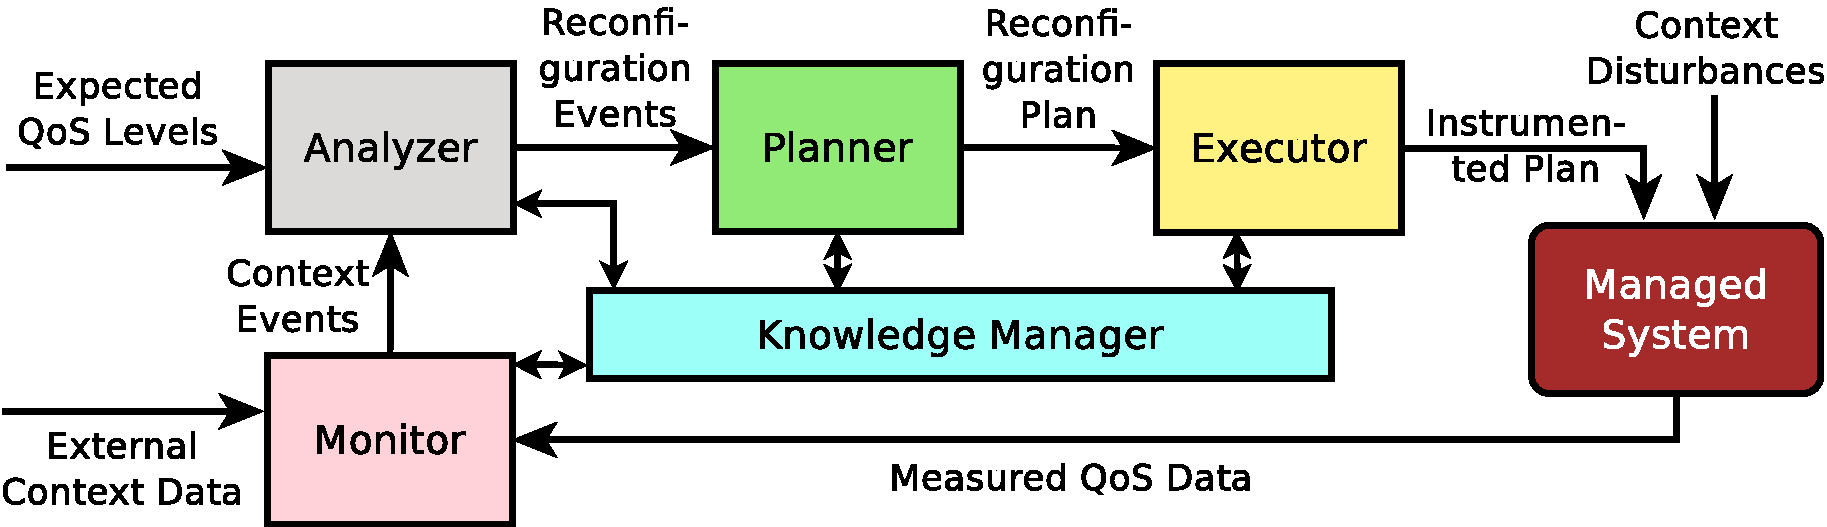
\includegraphics[width=0.95\textwidth]{fig/fback-loop-delta-dist}
	\caption{The MAPE-K reference model \cite{tamura:2012:QoS-CARE}}
	\label{fig:mape-k}
\end{figure}

\subsection {Self-Adaptive Software Systems}
As aforementioned in this document, self-adaptation is a capability of self-managed systems. Self-adaptive software systems are able to evaluate their own behavior and modify it in response to changes in their context (i.e., when these changes may imply that the system goals could not accomplished) or when achieving a better performance is possible \cite{tamura-et-al:2014:QoS-Contract-Preservation}\cite{villegas-et-al:2011:on-designing}. Because of this, self adaptive software systems are equipped with self monitoring components, analyzers, planners and executors. That is, they are usually based on the MAPE-K loop and technologies relying on component based architectures. Self-adaptive systems have been studied and applied in a wide variety of areas, such as systems evolution, object-oriented programming, autonomic computing, among others \cite{SEFSAS3:2017:what-can-control}\cite{villegas-et-al:2017-architecting-SwSystems-for-self-adaptation}\cite{Munoz-et-al:2015:refas-splc}\cite{Munoz-et-al:2015:variamos-splc}. However, the self-adaptive term is hard to distinguish from other terms, such as autonomic computing and self-management. According to \cite{Salehie:2009:SSL:1516533.1516538} the main difference between these terms is that autonomic computing includes a hierarchical set of layers required to administrate a software-intensive system: (i) application(s), (ii) middleware, (iii) network, and (iv) operating system, whereas self-adaptive systems are more limited and they only include layers (i) and (ii). However, in many cases these terms are used interchangeably.\\

Despite of there are numerous research about the Self-Adaptive software systems still there are many challenges around this topic \cite{de2013software}. The main challenges identified are:

\begin{itemize}
	\item Modeling dimensions: The objective of this challenge is to design models where a wide amount of systems properties could be represented to support the analysis and decision making processes.
	\item Requirements: The objective of this challenge is to capture the uncertain of any system through a language in an abstract level and interpreting this uncertain as a requirements collecting phase.
	\item Engineering: The objective of this challenge is to explicit the control loop role through the life-cycle of self-adaptive software systems (i.e., requirements, analyses, design, development, deployment, and operation of not only the system but also the control loop).
	\item Assurances: The objective of this challenge is to develop models that allow supplement the traditional V\&V methods to respond effectively to the dynamic context of the self-adaptive software systems.
	\item Design space for adaptive solutions: The objective of this challenge is to define a design space during the life-cycle of the self-adaptive software systems and the decisions that the software architect should address. In traditional life-cycle this space and these decisions are distributed through all process but these are centered in the analysis and design phases. However, in the self-adaptive software systems is more complicated to define this space due to its dynamic character.
	\item Processes: The objective of this challenge is to propose a process to develop a self-adaptive software system, this process should considerer dynamism involved by self-adaptive software systems.
	\item From centralized to decentralized control: The objective of this challenge is to design control schemes for centralized and decentralized structures defined a systematic way for software adaptation.
	\item Practical run-time verification and validation: The objective of this challenge is to investigate V\&V methods that allows gathering inferential assessment data to provide trust in self-adaptation process.
\end{itemize}

\subsection{Self-* Properties}

%\todo{DEBES reescribir los parrafos de esta seccion, porque son copy-paste de otro paper}

Self-* properties are the properties to be maintained by adaptation processes, introduced by Kephart and Chess in the vision of autonomic computing \cite{autonomiccomputing} in order to specify the aspects or attributes of self-managed systems, these are defined as follows: \\

\noindent\textbf{Self-Configuring.} This property defines that system must configure dynamically to accomplish with high-level policies specified in the service level agreements (SLAs). \\

\noindent\textbf{Self-Optimization.} This property defines that system must monitor and tune itself in an automatic way with the aim of improve its operation to satisfy needs of the end-user and business goals.\\

\noindent\textbf{Self-Healing.} This property defines that system must detect, diagnose, and repair any fail or malfunction of software found itself without the end-user perceives it or to affect the system execution. \\  

\noindent\textbf{Self-Protection.} 
This property defines that system must anticipate, detect, and identify potential threats that arise in its internal or external context and protect itself of them. \\

In terms of the self-* properties, our project will help in the advance of the achievement of the \textit{Self-Configuring} property, since the characterization of the system response in terms of latency and throughput performance factors of the relationship between design patterns and context-variables may guide the construction of the knowledge base component of SAS systems.


%\section {The \qoscare{} Framework}
%\qoscare{} is a reliable and robust reconfiguration framework that preserves QoS contracts in component-based software applications, which resulted from the PhD Thesis of Tamura \cite{tamura:2012:QoS-CARE}. The main goals of this thesis are: (i) to characterize properties of SAS systems and (ii) to provide a comprehensive solution to fulfill QoS contracts and preserve their fulfillment through dynamic reconfiguration. Relevant for our thesis proposal, the second specific result of Tamura's thesis is an evaluation framework for self-adaptive systems that defines a list of self-adaptation properties.

%In this section we focus on \qoscare{}, which is the implementation of a software architecture defined according to a formal model to preserve QoS contracts fulfillment. This  model is based in two formal systems: (i) the theory of Finite State Machines (FSM) and (ii) the Typed Attributed Graph (also called e-graph) Transformation System (TAGTS) theory. The theory of FSM is used to specify the semantics of QoS contracts, and modeling the fulfillment and unfulfillment states of QoS contracts. The TAGTS theory allows to model the reconfiguration operations using design patterns in reconfiguration rules due to TAGTS capabilities such as graph-based pattern-matching and transformation.

%\qoscare{} conceives the reconfiguration mechanism in an independent way of the managed software. Moreover, following the SCA standard, this mechanism is also independent of component runtime platforms. Therefore, we plan to use this framework to integrate the results of our proposal in it. \qoscare{} was designed to leverage domain-specific design-patterns at runtime, in general. Our aim in this thesis proposal is to parameterize and fine-tune its analyzer, planner, and knowledge-base with performance domain-specific design-patterns. 

%\section {Systematic Literature Reviews (SLR)}
%Systematic literature review is a methodology to perform rigorous reviews of the current state of studies about a particular topic developed in a particular area of knowledge \cite{keele2007guidelines}. The systematic literature review methodology defines a review protocol to assure the validity of a literature review because it must be repeatable by any researcher with the same results. This protocol is focused in defining a set of research questions that address the identification, evaluation, selection, and synthesis of relevant information.

%\section {PaSCAni}

%\section {Amelia}

\section{Chapter Summary}
This chapter summarizes all required concepts to approach this thesis. We start with the quality attributes (focused on the performance quality attribute and its sub-attributes), next, defining the domain-specific design patterns, after, we define the context-aware computing. These three concepts are the base of the problem defined in section \ref{sec:ProblemStatement} . Additional concepts required to understand the work carried out in this thesis are the component-based software engineering and the autonomic computing, specifically the self-adaptive software systems.
	
	% =========================================================================
	\chapter{Modeling the Problem}
	\label{cha:modelingProblem}
	To have a better understanding of the problem statement defined in section \ref{sec:ProblemStatement} for this thesis, in this chapter we analyze and model it in detail.

There are three main dimensions involved in the problem statement: (i) context variables, (ii) domain-specific design patterns, and (iii) performance factors. In sections \ref{sec:dsdpModel}, \ref{sec:pfModel}, \ref{sec:contextVariablesSearch} we detail each dimension respectively. In the last section we analyze how these dimensions interact between them and how we model the problem taking account each dimension and their interactions.

\section{Context Variables}
\label{sec:contextVariablesSearch}

As introduced in section \ref{subsec:contextaware} the fulfillment of Quality Attributes and Service Level Agreements (SLAs) can be violated became of changes on context variables. To identify the most relevant context variables that affect the performance of software systems, we conducted two systematic searches. The first search was centered in extracting the context variables defined by the context section domain-specific design patterns identified in the systematic literature review described in section \ref{sec:SLR}. The second search was conducted through the search engine of the Engineering Village data base using the next search string.

In this search string we define that the study areas of the fuzzy logic, ubiquitous computing, embedded systems, artificial intelligence and wireless sensor networks are excluded from our search due to these are areas that require too specific conditions to apply any pattern, therefore, to generalize a pattern or use their patterns in another contexts could be a not trivial problem.  \newline

"((((((((((((((((((((((self-adaptive systems) WN ALL)) AND (context)))) AND (({ieee computer society} OR {springer verlag} OR {inst. of elec. and elec. eng. computer society} OR {institute of electrical and electronics engineers inc.} OR {elsevier} OR {elsevier inc.} OR {elsevier ltd}) WN PN)) AND (({ca} OR {ja} OR {cp}) WN DT)) NOT (({716} OR {921} OR {717}) WN CL)) NOT (({ubiquitous computing} OR {embedded systems} OR {artificial intelligence}) WN CV)) NOT ({portuguese} WN LA)) NOT (({fuzzy logic} OR {wireless sensor networks}) WN CV)) NOT ({461.9} WN CL)) NOT ({912} WN CL)) NOT (({913.1} OR {802.2} OR {802.3} OR {901.2}) WN CL)) NOT ({944} WN CL)) NOT (({711} OR {741.1} OR {902.2} OR {971} OR {913}) WN CL)) NOT (({461.6} OR {481.1} OR {741}) WN CL)) NOT (({901.1.1} OR {911}) WN CL)) NOT (({721} OR {911.2}) WN CL)) NOT (({401.1} OR {402} OR {405.2} OR {751.5} OR {811.1.1}) WN CL)) AND (({ca} OR {ja}) WN DT))" \newline

The first search produced the domain-specific design patterns catalog presented in section \ref{sec:SLRResults} and this second search produced 87 papers, of which 32 passed the abstract filter and were fully read. The only characteristic to considerer when we read papers was the appearance of the text context variable, so, if a paper did not mention at least one context variable, it was rejected. After full reading, context variables was gathered from only 15 papers. Following we presented all context variables found.

{\scriptsize 
	\begin{longtable}{|p{1.7in}|p{4.5in}|}
		\caption{Context Variables that affect the performance of software systems}\\
		\hline
		\centering\textbf{Context Variable}                 & \textbf{Definition} \\
		\hline
		\endfirsthead
		\multicolumn{2}{c}%
		{\tablename\ \thetable\ -- \textit{Continued from previous page}} \\
		\hline
		\centering\textbf{Context Variable}                 & \textbf{Definition} \\
		\hline
		\endhead
		\hline \multicolumn{2}{r}{\textit{Continued on next page}} \\
		\endfoot
		\hline
		\endlastfoot
		Number of available CPU cores                       &                     
		Nowadays CPUs have more than one core, which execute tasks
		in parallel. Available CPU cores can affect directly system performance by executing several system tasks concurrently.
		Therefore this is an important context variable.        \\ \hline
		Number of available distributed task processors     &                     
		This variable is similar to the number of available CPU cores, except it refers to physically distributed CPUs, that is, several system devices distributed and each one of these has their own set of CPU cores.           \\ \hline
		Power Consumption                                    &                     
		It refers to electric consumption of system devices used in the system architecture.            \\ \hline
		Network Utilization                                 &                     
		It can refer to two variables, (i) the amount (percentage) of network used by the deployed application, or (ii) the amount of network used by all applications deployed over the same network.           \\ \hline
		CPU Clock Frequency                                    &                     
		This variable amounts to the maximum number of CPU instructions executed per second. Thus, it affects directly performance of software execution in a single CPU.          \\ \hline
		Addition of Resources at Runtime                    &                     
		Ability of adding or removing devices to the system architecture or resources at current devices in use by the system.          \\ \hline
		Number of service request                           &                     
		The amount of user requests for system functionalities. This variable affects performance given that this amount represents the load of the software system. If the system has not enough resources to service the requests, the system can become too slow or fail overloaded.            \\ \hline
		Number of Users                                     &                     
		The amount of concurrent users that the application has in a given moment, related to the number of service requests.          \\ \hline
		Bus Width                                           &                     
		Amount of bits that can be transported at the same time through the data bus that communicates the CPU with the memory and I/O peripherals.          \\ \hline
		Operating System                                    &                     
		The specific way that the operating system uses to manage hardware resources and provides services to applications affects the performance of applications.          \\ \hline
		Processor Utilization                               &                     
		It can refer to two variables, (i) amount (percentage) of CPU used by the application deployed, or (ii) amount of CPU used by all applications deployed over the same device.           \\ \hline
		Available RAM Memory                                 &                     
		Availability of random access memory (RAM) to store both, the program and the data that are processed by the CPU. The more available memory has a processing node, the more computing power. Available RAM memory is an important context variable that affects software performance.             \\ \hline
		Temperature                                         &                     
		It refers to temperature CPU devices, when a device is overheated its performance could be adversely affected.           \\ \hline
		Network Bandwidth                                   &                     
		It refers to the bit-rate of transmission and reception of data over a network, usually expressed in bits per second.            \\ \hline
		Task Buffer size (Queue)                            &                     
		It refers to the maximum amount of tasks that a software component can remain waiting (on a queue) until attended.            \\ \hline
		Type of execution task (Sequential or Concurrent)   &                     
		It refers to dependencies between tasks. If there is a lot of dependency among tasks, then, it is too difficult to take advantage of concurrency, thus, affecting software performance.           \\ \hline
		Batch Time Span                                     &                     
		It refers to a time that a software component waits before starting next task. Time between tasks could allow to free computational resources and so the next task can take advantage of these resources. It could affect  applications performance.          \\ \hline
		Synchronous or Asynchronous Communication Among Application Components          &                     
		It refers to whether the application must wait for a response or not. If an application keeps occupied attending one request from start to end of request (synchronously), then, it can increase the time that an application needs to process one request. In contrast, if it receives all requests and  it responds each request whenever they been completely processed (asynchronously). However, if processing one request requires to synchronization constantly then it is better for the application performance to be synchronous.          \\ \hline
		Batch Size (Coarse, fine, and medium)              &                     
		It refers to task size for processing distribution. Deciding over batch size used to distribute work among processing units to complete a request can affect application performance. On the one hand, if batch size is too small, then, application does not take advantage of computational resources. On the other hand, if batch size is too big then computational resources could be overloaded.           \\ \hline
		Centralized or Distributed Control mechanism        &                     
		It refers to how is distributed the control mechanism, that is, using only one device or more than one for controlling the application. To have more than one controller could increase or reduce application latency to respond a request and therefore it can affect application performance.           \\ \hline
		Heterogeneous or Homogeneous tasks                  &                     
		It refers to task kind, when there is one or more kind of task. If there is only one kind of tasks, then it is more simple to add resources to reduce response time, otherwise, the architecture should describe one strategy to manage the different tasks looking to improve software performance. This variable can affect directly the scalability quality attribute being related to software performance because if requests  increase and the system can not scale, performance will be decreased.        \\ \hline
		Shared Memory Architecture (UMA, NUMA, COMA, NORMA) &                     
		It refers to how shared memory is accessed by software components. There are four architectures, (i) Uniform memory access (UMA), (ii) Non-uniform memory access (NUMA), (iii) Cache-only memory architecture (COMA), and (iv) No Remote Memory Access (NORMA). The way to access to memory can increase or decrease application latency, thus affecting software performance.           \\ \hline
		Stateful/Stateless information                                &                     
		It refers to whether software components manage computational states or not. Having state implies to keep information over each request, managing this information implies more complexity to software components and increases latency. Despite of a stateless system could have better performance than stateful systems, to resolve some software problems requires to maintain state.           \\ \hline
		Communication protocol between components           &                     
		It refers to communication protocols used in Service Component Architecture (SCA) or even in general distributed components communication. Self-Adaptive software systems are commonly based on SCA. There are different protocols, such as; Web Services, REST, RMI, WCF, CORBA, and Slice (ICE). Each protocol to communicate components implies a different overhead over transmitted data and therefore this context variable can affect performance.            \\ \hline
		Communication time                                  &                     
		It refers to the time that system components spend in communication with others. This variable can affect the time to service a request and software performance. It can be affected by variables such as network bandwidth, shared-memory architecture, communication protocol, or batch size. Therefore, this is an important context variable.          \\ \hline
	\end{longtable}
}


\section{Domain-Specific Design Patterns}
\label{sec:dsdpModel}

To date considerable amount of design patterns have been published. For example, Gamma \etal{} \cite{Gamma:1995:DesignPatternsBook} classified design patterns in three types, (i) creational, (ii) structural, and (iii) behavioral, characterizing a total of 23 design patterns. However, in this thesis we are interested in domain-specific design patterns, in the domain of performance. To characterize them, we performed a Systematic Literature Review (SLR) \cite{keele2007guidelines}. 

\subsection{The Systematic Literature Review (SLR)}
\label{sec:SLR}
To perform the SLR, we followed the steps defined in the methodology proposed by Kitchenham et al \cite{kitchenham2009systematic}, as follows:

\subsubsection{Research Questions}
\begin{enumerate}
	\item Which are the domain-specific design patterns that have been proposed to improve the performance in a software system?
	\item In what amount do these design patterns enhance the software performance?
	\item Which are the metrics or methods used to measure the performance improvement obtained by the implementation of these design patterns?
	\label{enum1}
\end{enumerate}

\subsubsection{Generating a search strategy for primary and secondary studies}

The primary and secondary studies are searched through search strings in recognized sources. To generate the search strings we define keywords and then we select sources.\\

We defined the keywords according to the research questions. First, the domain we are interested on for the design patterns is the quality attribute "Performance", hence, this is the first keyword. Moreover, the performance has sub-attributes such as throughput, scalability, and load balance, then these sub-attributes are added to the keywords. Second, we are focused on design patterns, therefore, design pattern is also a keyword. Third, the metrics and evaluations are important in our research questions, thus, performance metrics, quality metrics, quality attributes assessment, and quality attributes evaluation are included as keywords. Finally, the processing paradigm influences in the performance importance in the systems, thus, concurrency, distributed systems, distributed processing, and parallel systems also are keywords. Additionally, some synonyms are added.\\

The sources are defined in accordance with three criteria: (i) source reputation, (ii) accessibility, and (iii) expert recommendation. Additionally, even though the relationship between design patterns and quality attributes has been widely investigated, for the practitioners are still difficult to find guides that allow them to make decisions about which design pattern improves the required quality attribute for a specific software system given that those are qualitative studies. Thus, to avoid the shallowness in our SLR we focus on the quality attribute \textbf{\textit{Performance}} and the design patterns that improve this attribute, hence the sources should be recognized by research communities software engineering. \\

Additionally, the researchers adjust the search strings by making some initial searches for calibration  the sources.

\begin{itemize}
	\item Keywords: Performance, Throughput, Scalability, Design pattern, Load balance, Quality attributes, Quality improvement, performance metrics, quality metrics, concurrency, distributed systems, distributed processing, parallel systems, quality attributes assessment, quality attributes evaluation, reference models (for performance), architectural styles (for performance).
	
	\item Sources: Given of the wide spectrum of articles found in this topic, we decided to focus the search in the next sources:
	
	\begin{itemize}
		\item ACM Digital Library
		\item Springer- LNCS
		\item IEEE
		\item Elsevier
	\end{itemize}
	
	The next subsection (\nameref{subsec:searchstrings}) limits the search results for these sources.
	
	\label{enum2}
	
\end{itemize}

\subsubsection{Search Strings}
\label{subsec:searchstrings}
Search strings represent a valid combination of keywords for its use in editorial search-engines; the correctness of both keywords definition and search-string construction are fundamental to find relevant studies.

The search strings used in the selected sources are listed below

%\footnote{The considerations to transform the general search string to its equivalent in the different sources are detailed in chapter\ref{chap:search-and-filter}.}:

\begin{itemize}
	
	\item General String (i.e., without editorial format)
	
	(performance OR concurrency OR throughput OR scalability OR "load balanc*") AND ("design pattern*") AND (distribut* OR parallel OR quality OR improvement OR measur* OR evaluat* OR assessment) AND publication-year$\geq$2006 \label{seastr:general} 
	
	\item IEEE Xplore
	
	((((((((performance) OR concurrency) OR throughput) OR scalability) OR "load balanc*") AND ("design pattern*") AND (((((((distributed) OR parallel) OR quality) OR improvement) OR measure) OR evaluation) OR assessment)))) \label{seastr:IEEE} 
	
	\item ACM
	
	(Abstract:performance or Abstract:concurrency or Abstract:throughput or Abstract:scalability or Abstract:"load balancing") and (Abstract:"design patterns") and (Abstract:distribut* or Abstract:parallel or Abstract:quality or Abstract:improvement or Abstract:measurament or Abstract:evaluation or Abstract:assessment or Abstract:"reference model" or Abstract:"architectural style" or Abstract:metrics) \label{seastr:ACM} 
	
	\item Springer
	
	(performance OR concurrency OR throughput OR scalability OR "load balanc*") AND ("design pattern*") AND (distribut* OR parallel OR quality OR improvement OR measur* OR evaluat* OR assessment OR "reference model*" OR "architectural style*" OR metric*) \label{seastr:Springer} 
	
	\item Elsevier
	
	pub-date$>$2005 and tak(performance OR concurrency OR throughput OR scalability OR "load balanc*") AND tak("design pattern") \label{seastr:Elsevier} 
	
\end{itemize}

\subsubsection {Inclusion Criteria}
\begin{itemize}
	\item Published papers since 2006 (10 years seems to be reasonable spectrum of time)
	\item Studies that contains experiments regarding design patterns for a specific domain that improve the performance in software systems.
	\item Studies with theoretical models about the measurement of the performance in a software system.
\end{itemize}
\subsubsection {Control Articles And Documents}
\begin{itemize}
	\item Pattern-oriented software architecture \cite{Buschmann:1996:PSA}
	\item Patterns for parallel programing \cite{Mattson:2004:PPP}
\end{itemize}
\subsubsection {Selection Procedure}
This subsection illustrates the process performed to select the relevant results (i.e., papers) from the search. Special considerations from this process can be found in subsection \textbf{\emph{\nameref{subsub:searchandfilter}}}.

\begin{itemize}
	\item A first search is performed by the team, with the aim of both analyzing the results and refine the search criteria defined in previous steps.
	\item The sources are distributed among team members.
	\item Every member has to perform a individual re-search process in its assigned source. The quality assurance process is applied for every paper.
	\item Relevance of resulting papers are evaluated based on abstract content and inclusion criteria.
	\item Another member of the team performs a second evaluation of the paper.
	\item Papers who received double-acceptance from members are immediately considered for full-text revision. In cases where there is no agreement, a third evaluator takes participation. 
	\item Every member performs the strategy defined for data extraction in the abstract accepted papers.
	\item The team carries out a general review of the most significant results and selects the papers for deep analysis (i.e., full-text review).
	\item The information is synthesized in the dimensions of analysis. 
\end{itemize}
\subsubsection {Quality assurance process}

To determine if a study is relevant for us, this should accomplish some of the next characteristics:

\begin{itemize}
	\item The article must have at least one design pattern or strategy that improve performance.
	
	\item The article should present experiments that support the performance improvement achieved when the design patterns or strategies are implemented.
	
	\item The article should present a mathematical model that allows to predict the performance improvement achieved when the design patterns or strategies are implemented. Additionally, the article should present experiments that support the real performance improvement.
	
	\item The patterns or strategies presented are focused to improve the performance directly.
	
	\item More than one article presents the same pattern or strategy.
\end{itemize}

%\begin{enumerate}
%\item Experimental approaches
%\begin{enumerate}
%\item Experimental tables: How many data was experimented with?. How many experiments were conducted?
%\item The document shows how the experimental results were synthesized in a mathematical model.
%\end{enumerate}
%\item Mathematical Model approaches
%\begin{enumerate}
%\item Characterize the evaluated models.
%\item Experimentation with mathematical model .
%\end{enumerate}
%\end{enumerate}
\subsubsection {Extraction data strategy}
The following represent the characterization model applied for initial resulted papers.
\begin{itemize}
	\item Source (Editorial)
	\item Classification
	\item Authors and authors affiliations
	\item Summary
	\item Research questions
	\item Publication year
	\item Source type (Journal, magazine, book)
	\item Studied patterns
	\item Approach of the performance evaluation
	\item Amount reference 
\end{itemize}

\subsubsection {Synthesis strategy: Analysis Dimensions}
\begin{itemize}
	\item Performance Problem and Type of Improvement Strategy: This dimension describes context, problem, and strategies (i.e., reference model, architectural style, design pattern, meta-model, framework, or algorithm) used by the authors for improving performance. This present the next sub-dimensions:
	
	\begin{itemize}
		\item Named Strategies
		\item Problem
		\item Context
	\end{itemize}
	
	\item Performance Target: This dimension is focus on which performance sub-attributes (i.e., throughput, latency, and response time) are improved and which measures are used for these sub-attributes. 
	
	\item Strategy: This dimension presents the strategies described by the article authors according to the next characteristics:
	
	\begin{itemize}
		\item Name
		\item Intent
		\item Problem
		\item Context
		\item Forces
		\item Structure
		\item Behavior
	\end{itemize}
	
	\item Mathematical model/analysis: If the article contains a mathematical model, this dimension presents its variables and its formulas.
	
	\item Experimental evaluation: This dimension presents the article experiments according the next characteristics:
	\begin{itemize}
		\item Case of Study
		\item Application Domain
		\item Experiment Setting (i.e., system deployment configuration, benchmark, scenarios, or data).
		\item Results
	\end{itemize}
	\item Relationship between experimental evaluation and mathematical model (if any).
\end{itemize}

\subsubsection{The Search and Filter Process}
\label{subsub:searchandfilter}
The search process starts with the definition of the sources and keywords; once sources have been selected based on selection criteria and keywords are correctly joined to form a representative search string. We faced to transform the general search string (i.e., search string \#\ref{seastr:general}) to the different sources search-options and their interfaces. The differences among the sources forced us to both increase or decrease the stiffness of search strings.

We present the most significant considerations and issues that we faced in search process.

\begin{itemize}
	\item Elsevier
	
	The search engine of Elsevier is called \textit{ScienceDirect}. ScienceDirect presents two options for advanced search; these are \textit{Advanced search}, and \textit{Expert search}. For the purpose of the current research, we decided to use the Expert search, which allow us to represent our general search string with few modifications. However, due to the results of the original search were few (i.e., less than 30), the stiffness of the search string had to be decreased. After some iterations, we agree to use query string \#\ref{seastr:Elsevier}.
	
	\item Springer
	
	Springer advanced search restricts the reach of our search significantly; first, Springer does not present a query search mode as ScienceDirect expert search. Because of this, we were forced to limit the search to the field \textit{Where the title contains}. This evidently, produces a high number of initial results. Second, In order to select relevant results was necessary to use filters that can only be added in a step-by-step form using \textit{Refine your search} option. In summary, the process performed in Springer was:
	\begin{itemize}
		\item The search string \#\ref{seastr:Springer} is typed in the field “where the title contains”.
		\item In the field \textit{Show documents published} set: 2006 between 2014.
		\item Add discipline filter: Computer Science.
	\end{itemize}
	
	It is important to mention that, given the fact that Springer search was limited to title search, relevant results could be omitted (but also irrelevant results could be considered) in comparison with other sources that allows the combination of title, abstract, and keywords in a single search.
	
	\item ACM and IEEE Xplore
	
	ACM and IEEE sources show the most complete advanced search mode in comparison with the previous sources; they bring the possibility to represent the exactly original query string with a few format modifications. The query strings used for ACM and IEEE was query string \#\ref{seastr:ACM} and \#\ref{seastr:IEEE}, respectively. Even though, both sources require that publication-year filters are added manually (i.e., after get results) the process is very simple and effective.
	
\end{itemize}


The filter process, that is refinement of results, starts with the 248 resulting papers from previous stage (i.e., search process), hereinafter known as initial search stage. In total, the filter process is composed by three iterative stages: (i) Initial Search, (ii) Abstract Accepted, and (iii) Full-Text Accepted. The general aim of each stage is to filter the irrelevant papers from current research. 

\begin{itemize}
	\item Initial Search
	
	In this stage, resulting papers from all sources are collected and distributed among researchers. As we mention before, 248 papers result from search process.
	
	\item Abstract Accepted
	
	In this stage, the papers are evaluated by the researchers based on the content of the abstract. If the paper fulfills the inclusion criteria, it receives the approbation from the researcher. However, a paper is only accepted in this stage (i.e., considered for the next stage) if two researchers agreed in the evaluation. It is important to mention that, some papers could not expose clearly the inclusion criteria in the abstract section; however some relevant information is detected in the same. Papers that meet previous condition are also accepted. 
	
	At the end of this stage, the 59 resulting papers are again distributed among researchers.
	
	\item Full-Text Accepted 
	
	In this stage, the papers are studied in depth with the purpose of finding its relevance for the current technical report. Researchers look for papers that fulfill inclusion criteria and quality assurance statements.
	
	At the end of this stage, only 20 papers were finally accepted, representing the starting point for the current document.
	
\end{itemize}

The resulting papers from last stage produce a snowball process. It consists on to select the most relevant references of the accepted papers with the aim of emphases or gather extra-information. The snowball process produced 15 new papers, nonetheless after applying the previous filters only 6 papers remained, for a total of 26 papers. Figure \ref{fig:filter-process} summarizes the filter process results.

\begin{figure}[ht!]
	\centering
	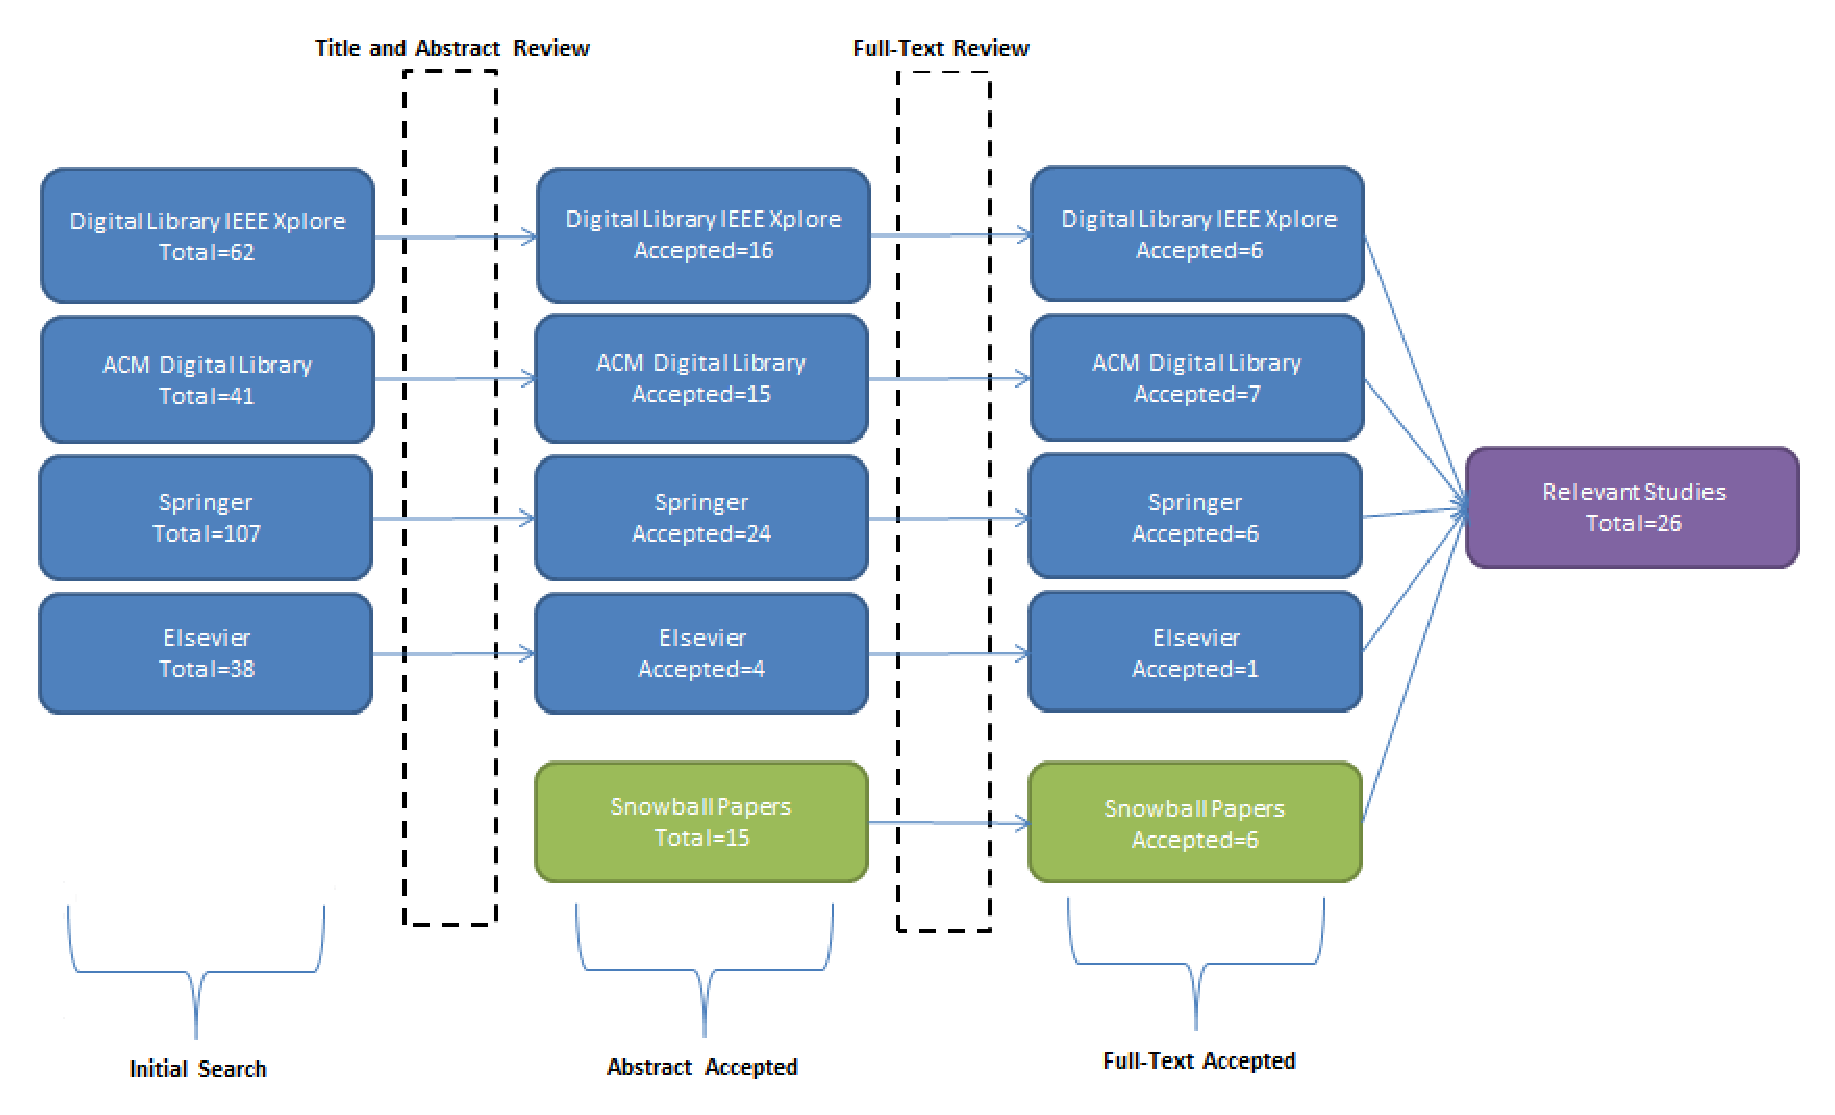
\includegraphics[width=17cm]{fig/filter-process.eps}
	\caption{Filter-Process Stage Results}
	\label{fig:filter-process}
\end{figure}

% =============================================================================

\subsection{SLR Results}
\label{sec:SLRResults}
The results of SLR were sorted according to their relevance and we develop a template to analyze each pattern through the next characteristics: (i) Intent, (ii) Problem, (iii) Context, (iv) Forces, (v) Structure, and (vi) Behavior.


\begin{description}
	\item [Intent] 	The intent is a short statement that summarizes what is the purpose of the design pattern, its rationale, and what particular design issue it address [Ref]. Optionally, The intent could include a brief explanation about how the design pattern solves the problem, and in which context. The intent allows practitioners to make decisions about the design pattern applicability.
	\item [Problem] Describes the specific problem addressed by the pattern. The problem is usually exposed with a proper scenario that exemplifies how the pattern is useful.
	\item [Context] The context establishes the set of conditions and the environment under which the problem appears for the pattern to be applied effectively.
	\item [Forces] Forces are generalized criteria justifying using and implementing a design pattern. Forces are generally hard to measure and conflicting between them. They are expected to occur repeatedly in the design pattern's context, and to resolved themselves under certain configuration (i.e., the pattern) [C. Alexander]. Forces can focus in different relevant aspects of patterns, for example, correctness, structure or construction. \\
		
%	[1] http://www.cs.unc.edu/~stotts/723/patterns/forces.html"
	\item [Structure] The structure describes the elements that compose the solution proposed by the design pattern, their relationships, and responsibilities. The structure description does not represent a specific implementation because the structure of the design pattern is intended to be a template. The structure is expressed through a class diagram conforming to the UML specification.
	\item [Behavior] The behavior describes the relationships and collaborations between elements defined in the pattern structure. The behavior is defined through a sequence diagram conforming to the UML specification.
\end{description}

Following are described the twelve more relevant design patterns for performance that were found in the SLR.


\subsection{Random Access Parser Design Pattern}

\subsubsection{Intent}
The Random Access Parser design pattern creates a navigable data structure from plain and large files that follows certain format, making it easier to access data records in both directions, backward and forward, while operating over them. Navigating the data structure produces per-record snapshots that are written to disk, which reduces reading time and memory consumption.

\subsubsection{Problem}
Usually, processing a large file of structured data (e.g., XML or JSON) requires different kinds of operations, for example, to insert, remove, and update data records in a data base management system. The structured data can follow a standard format, typically some conceptual variation of the WebRowSet format. The WebRowSet format comprises three parts: properties, metadata, and data. In the context of the previous example, the properties section contains details regarding the Relational Database Management System (e.g., synchronization provider, isolation level, and rowset type). The metadata section contains information about the database structure (e.g., column numbers, their names, and types). Finally, the data section contains the application data.

For the processing, data records might be required to be accessed randomly and refer to other records, located possible far before or after the current one. Another example is if a file can be processed per table, this requires to read not only the concrete data but also the associated metadata and properties. In case the metadata or properties are modified, it is likely the data would need to be also modified; performing such modifications imply moving forward and backwards in the file, therefore this can introduce performance issues. These issues are commonly caused because an efficient processing would imply to load the whole file into memory, which is not possible.

\subsubsection{Context}
Typical processing of data sets requires to iterate over the data records. Even though these data sets may be very large, a common approach is to load all the data into main memory. However, this affects negatively the overall application performance, and in some cases, it is not even possible to load the whole file into memory. For this reason, on-demand reading is desired and sometimes, required. Moreover, this strategy allows the processing to behave scalable and stable, in terms of time and memory consumption.

\subsubsection{Forces}
\textbf{\textit{Efficiently random access to a large structured data file.}} This design pattern proposes the use of two lookup tables. On the one hand, one table is used to remember the already read, updated, inserted, or deleted data records through parser snapshots using the memento design pattern. On the other hand, the other table is used to maintain the original data structure. These snapshots allow an efficient and manageable random access and avoid memory overflow caused by the processing of large files.

\subsubsection{Structure Diagram - Figure \ref{fig:str_diagram_rap}}

\begin{figure}
	\centering
	\includegraphics*[width=1\textwidth, keepaspectratio=false]{fig/image1.eps}
	\caption{Structure Diagram - Random Access Parser Design Pattern}
	\label{fig:str_diagram_rap}
\end{figure}

\begin{description}
	\item[Participants]
\end{description}

\begin{description}
	\item[Domain Specific Parser:]
	An abstract class that contains the abstract method \textit{parse}. This method allows to transform the contents of a file into a data structure, for instance, the corresponding data structure for the XML or JSON formats.
	
	\item[Concrete Parser:]
	A concrete implementation of the DomainSpecifParser class. It is responsible for implementing the \textit{parse} method. Some well known implementations of the ConcreteParser class can be found for XML-parsing libraries such as SAX, Dom and XPath.
	
	\item[Lookup Table:]
	This component allows to navigate inside memento snapshots.
	
	\item[Table Element:]
	This component is responsible to encapsulate and identify each memento element.
	
	\item[Memento:]
	Memento is a design pattern designed to save a specific object state. Given that the object states are saved, it can roll back to a previous state.
	
	\item[Random Access Parser:]
	This is the main component. It is responsible for reading a file, transforming it into a data structure by means of a ConcreteParser, performing operations (i.e., update, delete, insert) over the data structure, storing and restoring states of the data structure.
	
\end{description}

\subsubsection{Behavior}

%\begin{figure}
%	\centering
%	\includegraphics*[width=0.8\textwidth, keepaspectratio=false]{fig/image2.eps}
%	\caption{Initialization Sequence Diagram - Random Access Parser Design Pattern}
%	\label{fig:init_seq_diagram_rap}
%\end{figure}

\begin{figure}
	\centering
	\includegraphics*[width=1\textwidth, keepaspectratio=false]{fig/image3.eps}
	\caption{Processing Sequence Diagram - Random Access Parser Design Pattern}
	\label{fig:proc_seq_diagram_rap}
\end{figure}

%\begin{description}
%	\item[Scenarios]
%\end{description}

\begin{description}
	%	\item[Initialization Scenario - Figure \ref{fig:init_seq_diagram_rap}]
	%	This scenario describes how the design pattern is configured initially. To configure initially the design pattern a request to process a file must arrive, when file path is sent to RandomAccessParser, it calls the concrete parser for interpreting the file and the parser returns the corresponding DataStructure.
	
	
	\item[Processing Scenario - Figure \ref{fig:proc_seq_diagram_rap} ].\\
	This scenario describes the normal processing behavior of RandomAccessParser design pattern.
	
	\begin{itemize}
		\item  When any record is requested, no matter its location, RandomAccessParser searches into its LookUpTable the required element.
		
		\item  The LookUpTable searches in its TableElements the right element according to the elementId.
		
		\item  Once the correct TableElement is found, it gets its associated Memento object, and the memento is returned to the RandomAccessParser, which returns the DataStructureRecord.
	\end{itemize}
	
\end{description}

\subsection{Reactor Design Pattern}

\subsubsection{Intent}
The Reactor design pattern handles different types of concurrent service requests that are delivered by one or several clients. Service requests are received by a service-specific event handler, working separately from the service implementation. These event handlers are registered into a dispatcher, which is in charge of executing the corresponding services.


\subsubsection{Context}
A server application concurrently serves several types of service requests from one or more distributed clients. These requests are internally handled as events by event handlers.


\subsubsection{Problem}
In distributed environments, servers offer different services, and a single server can receive different request types. Processing a request can imply locks in the requests arrival point, while client requests are serviced. These locks can impact negatively the system performance.

Additionally, different request types require different handlers, hence it is necessary to select the adequate ones. This selection performed dynamically increases the time to respond each request. A typical solution is to use a thread for each request, however this solution implies system overhead when threads finish processing and become idle, especially when requests are not uniformly distributed among request types.


\subsubsection{Forces}
\textbf{\textit{Favor service availability. }}This pattern uses a dispatcher to redirect requests to the corresponding handlers, therefore the server does not block while attending a single request. \\

\noindent\textbf{\textit{Increase server efficiency.}} By using a request dispatcher, and by avoiding idle threads in request processing this pattern aims at reducing unnecessary use of CPUs and minimizing latency in service requests, and maximizes throughput.\\

\noindent\textbf{\textit{Ease service adaptability.}} Given that handlers are registered with a single request dispatcher, this pattern eases modifying or adding handlers for different types of service requests.

\subsubsection{Structure Diagram - Figure \ref{fig:str_diagram_r}}

\begin{figure}
	\centering
	\includegraphics*[width=1\textwidth, keepaspectratio=false]{fig/image4.eps}
	\caption{Structure Diagram - Reactor Design Pattern}
	\label{fig:str_diagram_r}
\end{figure}


\begin{description}
	\item[Participants]
\end{description}

\begin{description}
	\item[Request Processor:]
	Represents the requests reception point. This class contains the necessary information to redirect the request to the corresponding handler to process the service request.
	
	\item[Request Handler Interface:]
	An interface specifying the required service to handle requests. The service specified by this interface must be implemented by concrete request handlers. 
	
	\item[Concrete Request Handler:]
	A concrete class implementing the request handler interface.  Concrete request handlers are registered with the initiation dispatcher. When a request corresponding to the request handler type arrives, it is called by the initiation dispatcher.
	
	\item[Synchronous Request Demultiplexer:]
	Waits for a request to occur, and returns a handler without blocking the initiation dispatcher. Thus allowing the system to continue serving requests.
	
	\item[Initiation Dispatcher:]
	Responsible for both registering and removing request handlers, and dispatching service requests. It waits for requests to be processed by the synchronous request demultiplexer component, and calls the concrete request handler component to process each request.
\end{description}

\subsubsection{Behavior}

%\begin{figure}
%	\centering
%	\includegraphics*[width=0.8\textwidth, keepaspectratio=false]{fig/image5.eps}
%	\caption{Sequence Diagram Initialization - Reactor Design Pattern}
%	\label{fig:seq_diagram_r}
%\end{figure}

\begin{figure}[ht!]
	\centering
	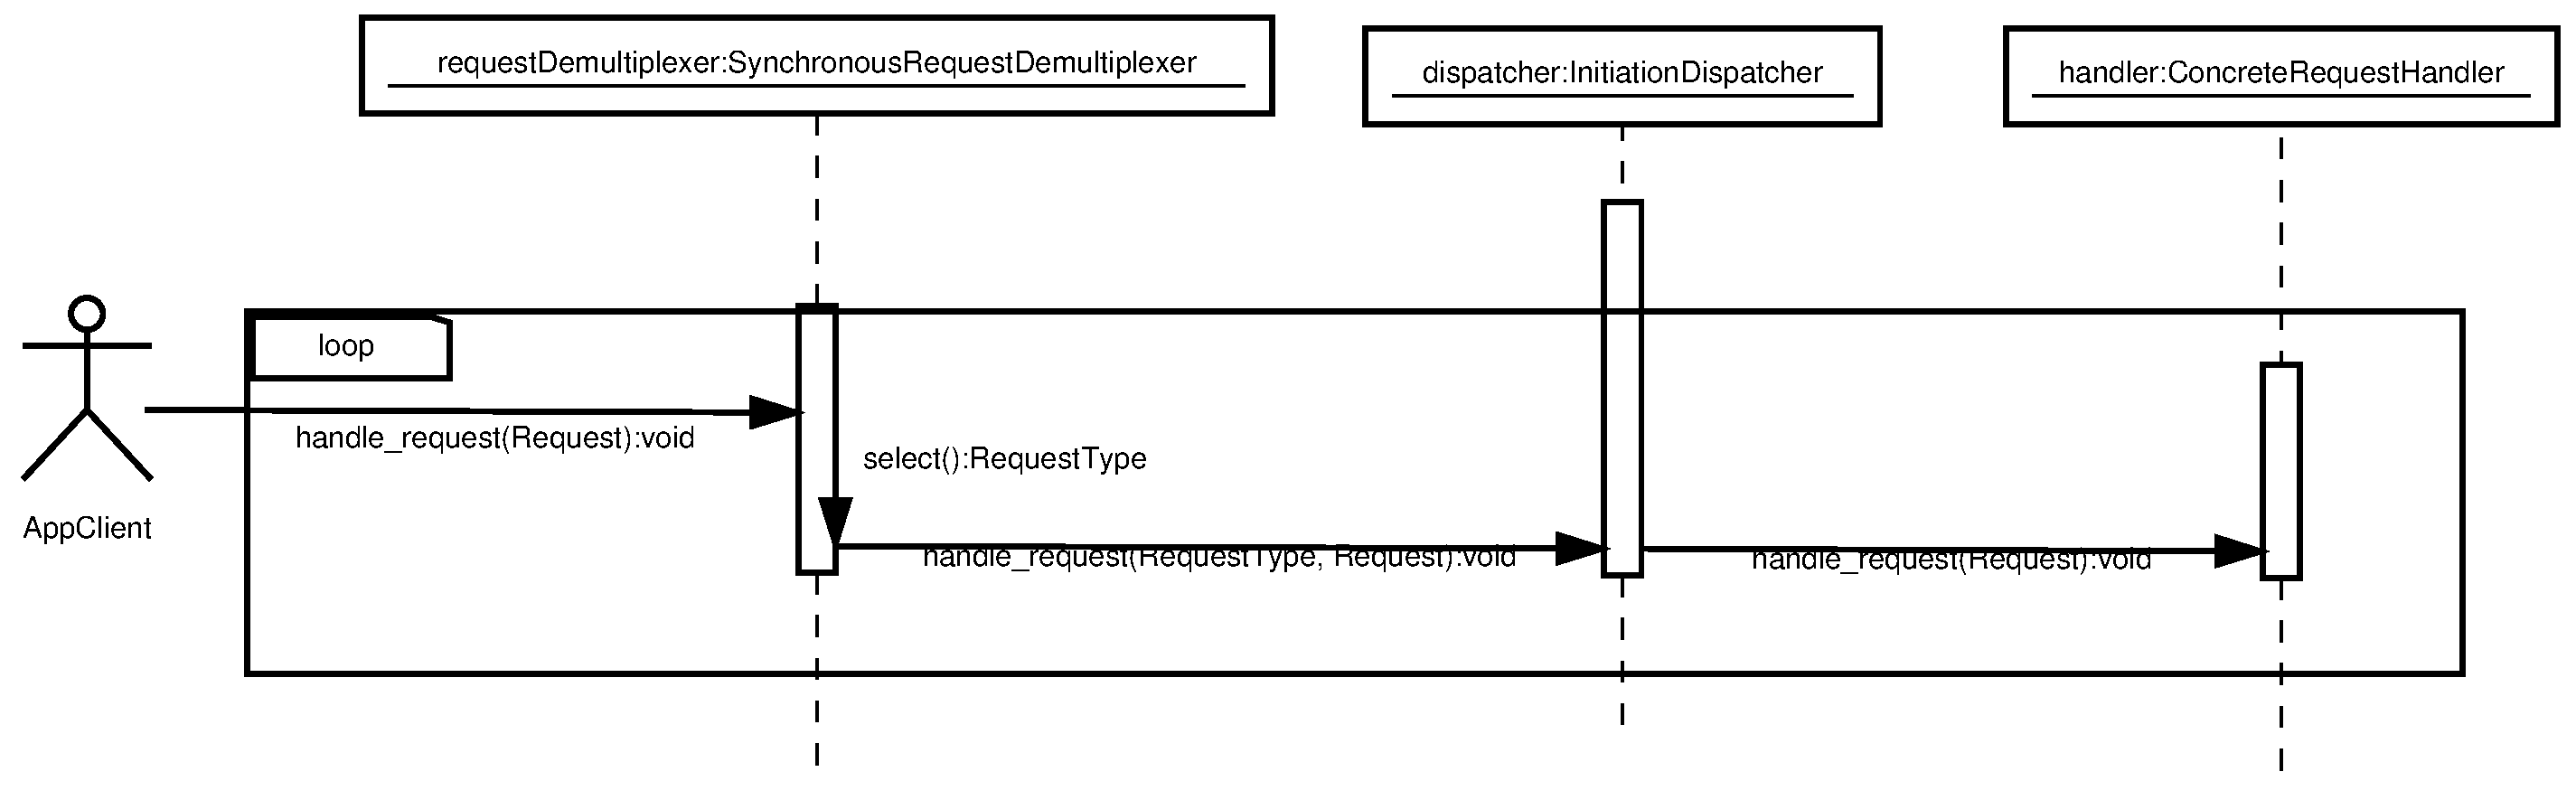
\includegraphics[width=1\textwidth]{fig/image32.eps}
	\caption{Request Processing Sequence Diagram - Reactor}
	\label{fig:seq_diagram_r2}
\end{figure}


%\begin{description}
%	\item[Scenarios]
%\end{description}

%\begin{description}
%	\item[Figure \ref{fig:seq_diagram_r} - Reactor Design Pattern]
%\end{description}

\begin{description}
	\item[Processing Scenario - Figure \ref{fig:seq_diagram_r2}].\\
	
	\begin{itemize}
		\item  When an Event handler is registered in the Initiation dispatcher, a type of event is specified by the application registering the handler; when an event of this type occur on the associated Handle, the Event handler will be notified.
		
		\item  The Initiation dispatcher gets the associated Handle from Event handlers once they are registered.
		
		\item  After all the Event handlers are registered, the event loop is started in the Initiation dispatcher by an application. So, the Synchronous event demultiplexer is executed and it is put on wait for events.
		
		\item  When a new event arrives (i.e., a Handle becomes ``ready''), the Synchronous event demultiplexer notifies the Initiation dispatcher.
		
		\item  When the Initiation dispatcher is notified about a new event, it calls the corresponding Event handler callback method. The initiation dispatcher uses the Handles to find the appropriate Event handler callback method.
		
		\item  The Initiation Dispatcher calls back to the handle event hook method of the Event Handler to perform application-specific functionality in response to an event.
	\end{itemize}
\end{description}

\subsection{State-based Pipeline Design Pattern}

\subsubsection{Intent}
The State-based Pipeline design pattern takes advantage of the simplicity of the Pipeline design pattern, and the efficient execution of a master/slave structure. This variant of the original pipeline design pattern reduces prominent downsides for coarse--grained applications in achieving good performance, namely: first, when the pipeline is not full (i.e., at the beginning and end of the pipeline) stages are idle; second, load balancing is crucial to achieve good performance, as expensive stages cause that less expensive stages stay idle; and third, it is difficult to incrementally add more processors into an existing pipeline, given that concurrency in a pipeline is tightly coupled with the set of stages.

\subsubsection{Problem}
The pipeline structure has demonstrated to be a useful way to solve many practical problems in parallel computing programming; however, it presents three serious problems, especially for coarse-grained applications. 

\begin{itemize}
	\item  Processors are idle when the pipeline is at the beginning and the end of the process.
	      
	\item  Traditional pipeline implementations are sensitive to load imbalance, this means that some pipelines stages are more time-consuming than others. The slowest stage will become a bottleneck, decreasing the performance.
	      
	\item  Traditional pipeline implementations imply static assignment of the stages to the nodes, making difficult to take advantage of new nodes.
\end{itemize}

\subsubsection{Context}
A pipeline consists of a set of ordered stages, where each stage receives data from its predecessor, transforms that data, and finally sends it to the next stage. Usually, for data transference it is necessary to place buffers between the stages.

The paramount characteristic in pipeline is that each stage is independent. That is, each stage can perform different computations on different parts of the data, simultaneously.

However, Pipeline presents serious performance problems as ramp-up and ramp-down time, and load imbalance. 

The state-based pipeline should be used when:

\begin{itemize}
	\item  Load balance must be guaranteed.
	      
	\item  New processor or stages could be available at any time and should be taken advantage of.
\end{itemize}

\subsubsection{Forces}
\textbf{\textit{Decouple the concurrency from the pipeline structure}}. By using the State-based Pipeline design pattern, stages (i.e., state transitions) are independent of the execution thread, improving load balancing between pipeline stages and reducing idle times.\\

\noindent\textbf{\textit{Clarify transitions between stages}}. There should be a clear agreement on the order in which the transformations occur from one stage to another. Thus if it is required, this makes it simple to add, modify or reorder states in the pipeline.

\subsubsection{Structure Diagram - Figure \ref{fig:str_diagram_sbp}} 

\begin{figure}
	\centering
	\includegraphics*[width=0.9\textwidth, keepaspectratio=false]{fig/image6.eps}
	\caption{Structure Diagram - State-based Pipeline Design Pattern}
	\label{fig:str_diagram_sbp}
\end{figure}


\begin{description}
	\item[Participants]
\end{description}

\begin{description}
	\item[AbstractStage]
	An abstract representation of the stages, containing an abstract method to transform one stage into another.
	
	\item[ConcreteStage]
	Represents a stage within the pipeline. Its method returns a concrete stage (the subsequent stage).
	
	\item[Pipeline]
	This class contains the configured concrete stages, the queues storing intermediate states (i.e., instances of ConcreteStage), and the slave threads consuming objects from the queues.
	
\end{description}

\subsubsection{Behavior}

\begin{figure}
	\centering
	\includegraphics*[width=1\textwidth,, keepaspectratio=false]{fig/StateBehavior.eps}
	\caption{Processing Sequence Diagram - State-based Pipeline Design Pattern}
	\label{fig:seq_diagram_sbp}
\end{figure}

%\begin{description}
%	\item[Scenarios]
%\end{description}

\begin{description}
	\item[Processing Scenario - Figure \ref{fig:seq_diagram_sbp}]
\end{description}

\begin{itemize}
	\item  Put the request objects into the input buffer.
	      
	\item  An idle thread from the thread pool will find and execute the transform() method of any object request from any buffer placed between stages, in order to obtain the next state object.
	      
	\item  The state object resulting from transform () method is placed into an output buffer proper of its runtime type.
	      
	\item  The final buffer holds the resulting output objects from the pipeline execution.
\end{itemize}

\subsection{Thread Pool Design Pattern}
\label{subsec:threadpool}

\subsubsection{Intent}
The thread pool design pattern facilitates thread management. In parallel environments, where some tasks can be executed at same time but perhaps in different instantiations, in the same device, threads should be used. Each thread executes an own task and shares device resources. When many threads are executed in the same device concurrently, resources could not be enough and overrun device capacity. 

\subsubsection{Problem}
Concurrency is usually realized having several threads executed in a computing device. However, each of these threads consume device resources, and eventually, many threads might overload the device. Managing these threads represents a problem. For example, Can threads be reused? What would be the maximum or minimum amount of threads for device?

\subsubsection{Context}
In general, each time a problem solution requires using concurrent execution of threads, this pattern can be used. Threads are used to execute several independent computing tasks at the same time, however these threads imply costs in time (i.e., time to start a thread) and resources (memory and CPU). This pattern proposes a solution that balances the implications of using threads. Furthermore, many other patterns that imply the use of threads implement this pattern as part of their solution. This is the case for instance with the leader/followers and master/workers design patterns.Despite of this pattern allows to take advantage of the multi-core environment of a CPU and this can improve the system performance, it has limitations, such as, difficult to scale the pattern implementation to a distributed environment (i.e., applying this pattern using many processing nodes).

\subsubsection{Forces}
\textbf{\textit{All tasks should be independent}}. Each of the tasks should be executable fully and independently in one thread. If there are dependencies, deadlocks can happen. For instance, if all pool's threads is waiting for other task, this task will not be executed and thus threads could enter in deadlocks.\\

\noindent\textbf{\textit{Thread creation cost is relatively high}}. To create a thread for each task should be costlier than maintaining and waiting for idle threads, both in terms of time and resources.\\

\noindent\textbf{\textit{Optimal threads amount}}. Designer should configure the optimal threads amount depending on the device resource availability and execution capability at the same time. This relation should be maintained dynamically, as the device load evolves.\\

\noindent\textbf{\textit{Threads not reusable.}} If a task lasts indefinitely, the thread that executes this task is not reusable because it may never terminate to execute the task. This task type should be executed by a thread out of pool.

\subsubsection{Structure Diagram - Figure \ref{fig:str_diagram_tp}}

\begin{figure}
	\centering
	\includegraphics*[width=0.7\textwidth, keepaspectratio=false]{fig/image8.eps}
	\caption{Structure Diagram - Thread Pool Design Pattern}
	\label{fig:str_diagram_tp}
\end{figure}

\begin{description}
	\item[Participants]
\end{description}

\begin{description}
	\item[Worker:]
	Responsible to execute tasks of ThreadPool. This gets Runnable objects from its ThreadPool, by executing the Runnable method.
	
	\item[Runnable:]
	Represents the interface implemented by tasks that ThreadPool must process. This interface specifies the \textbf{\textit{run }}method, which is responsible for defining the task of the Runnable object.
	
	\item[ThreadPool:]
	ThreadPool class is responsible for managing workers and tasks and their execution. This class assigns to each worker one task. When a worker finishes a task execution, it can ask the threadpool for a new task. 
	
	\item[Executor:]
	Represents the interface implemented by ThreadPool class. This interface specifies the \textbf{\textit{execute }}method, which is responsible for executing the task of the Runnable object.
	
\end{description}

\subsubsection{Behavior}

%\begin{figure}
%	\centering
%	\includegraphics*[width=1\textwidth, keepaspectratio=false]{fig/image9.eps}
%	\caption{Sequence Diagram Initialization Scenario - Thread Pool Design Pattern}
%	\label{fig:seq_diagram_tp1}
%\end{figure}

\begin{figure}
	\centering
	\includegraphics*[width=1\textwidth, keepaspectratio=false]{fig/image30.eps}
	\caption{Request Processing Sequence Diagram - Thread Pool}
	\label{fig:seq_diagram_tp2}
\end{figure}


%\begin{description}
%	\item[Scenarios]
%\end{description}

\begin{description}
	%	\item[Initialization - Figure \ref{fig:seq_diagram_tp1}]
	%	The initial configuration of this pattern depends on requests to execute tasks, every time a request arrives it is verified if idle threads exists, otherwise, if the maximum thread amount is not exceed, a new thread is created.
	
	\item[Processing Scenario - Figure \ref{fig:seq_diagram_tp2}].\\
	Every time a request arrives it is verified if idle threads exists, otherwise, if the maximum thread amount is not exceed, a new thread is created. If exists at least one thread available to process a request, the pool sends the request to be executed, otherwise the request must wait until a thread become idle. Finally, the thread returns to the pool as idle thread when processing of the request is finished.
\end{description}


\subsection{Master-Worker Design Pattern}
\label{sebsec:mw_design_pattern}
Also known as:

\begin{itemize}
	\item  The Embarrassingly Parallel Pattern
	\item  Task Queue
	\item  Master-Slave
\end{itemize}

\subsubsection{Intent}
The Master-Worker design pattern describes how to execute a collection of independent tasks (i.e., tasks than can be executed concurrently) in a group of available processors, named workers. Furthermore, the distribution of tasks among processors can be performed statically or dynamically in order to promote a balanced computational load.

\subsubsection{Problem}
Many computational problems are solved by splitting them in independent subproblems, such that their solution implementations can be executed independently and concurrently. The independence among subproblems imply that tasks associated to each solution implementation do not share read and write data and tasks must not wait for other task results. Practitioners should take advantage of available computational resources and the inherent concurrency without incurring in unnecessary overhead. Given this situation, a program should be designed procuring to load balance among available processing units.

To exemplify this type of problems, take the vector-addition problem. Given vectors A, B, and C where C=A+B, each element of C is given by adding the corresponding elements of A and B, Ci= Ai + Bi. Each element of C can be calculated in a concurrent way as a set of subproblems of vector elements addition problem.

\subsubsection{Context}
Problems whose solutions can be split in independent tasks can take advantage of this design pattern. However, some particularities should be evaluated before to implement it, (i) cost to initialize workers (including e.g., data transmission) must be lower than the task cost, (ii) number of tasks must be greater than available processing units, and (iii) distribution should be dynamic if load for each task is unknown, or varies unpredictably or when the available load supported by each worker is unknown.

\subsubsection{Forces}
\textbf{\textit{Task must be independent.  }}The Master-Worker design pattern applies when tasks do not have dependencies among them. Otherwise, the tasks must be redesigned to eliminate these dependencies.\\

\noindent\textbf{\textit{Tradeoffs between data communication and load. }}To apply this design pattern the task size must be optimal according to tradeoffs between distribution overhead and task implied load. Given that the size of tasks in Master-Worker can vary from one task to another. \\

\noindent\textbf{\textit{Unpredictable tasks number and processor nodes. }}Most of the time explicit predictions of the hardware and software runtime environment are not possible. However, Master-Worker procures to achieve load balancing even under uncertain environments, by allocating tasks to idle processor nodes. This scenario corresponds to the dynamic version of Master-Worker and also to the Fork-Join design pattern.\\

\noindent\textbf{\textit{Number of tasks and processor nodes are known. }}When the number of tasks and load of processor nodes is known prior to execution, practitioners can program the software to assign statically tasks to the most suitable processor node guaranteeing load balancing. This scenario corresponds to the static version of Master-Worker\footnote{ Some authors do not consider the behavior described by the static version of the Master-Worker design pattern as part of this design pattern, instead they prefer to describe this behavior as a whole new design pattern.}.

\subsubsection{Structure Diagram - Figure \ref{fig:str_diagram_mw}}

\begin{figure}
	\centering
	\includegraphics*[width=0.8\textwidth, keepaspectratio=false]{fig/image7.eps}
	\caption{Structure Diagram - Master-Worker Design Pattern}
	\label{fig:str_diagram_mw}
\end{figure}


\begin{description}
	\item[Participants]
\end{description}

\begin{description}
	\item[Master]
	\label{it:masterdesc}
	The Master contains the shared collection of tasks, usually a queue, where tasks are stored after being split.  It has a second shared queue where results of worker computations are stored. In summary, the Master holds registered tasks, launches the processors (workers) and collects the workers' results to produce the final result.
	
	\item[Worker]
	\label{it:workerdesc}
	Workers request a task from the shared collection of tasks registered in the master's queue, and process it. Finally, workers return partial results of the computation to the master.
\end{description}

\subsubsection{Behavior}
\label{subsubsec:beh_mw_design_pattern}

\begin{figure}
	\centering
	\includegraphics*[width=0.6\textwidth, keepaspectratio=false]{fig/image29.eps}
	\caption{Processing Sequence Diagram - Master-Worker Design Pattern}
	\label{fig:seq_diagram_mw}
\end{figure}

%\begin{description}
%	\item[Scenarios:]
%\end{description}

\begin{description}
	
	\item[Processing Scenario - Figure \ref{fig:seq_diagram_mw}]
	This scenario describes the usual processing behavior of Master / Worker design pattern. 
	
	\begin{itemize}
		\item  When a master launches workers, they request tasks to the master.
		
		\item  When a task is assigned to a worker, it processes the task and returns the result to the master.
		
		\item  When the worker finishes to process its current task, it will request for a new task to the master until all tasks have been processed and then the master shutdown all workers.
	\end{itemize}
	
	\item[Finishing - Figure \ref{fig:seq_diagram_mw}]
	This scenario describes how the Master / Worker design pattern is finished.
	
	\begin{itemize}
		\item  When all tasks have been processed, the master processes the collected partial results and returns the final result, if necessary, the master shuts down all workers.
	\end{itemize}
	
	\textbf{Special circumstances and variations. }
	
	\begin{itemize}
		\item  Usually problem's tasks return their results to the master, however this pattern can use a shared data structure to accumulate the partial results.
		
		\item  Termination condition is met usually when all tasks are completed, however there are problems whose final result can be obtained before all tasks are completed. For instance, a search in a database where each worker has an independent search space is finished as soon as the first worker finds the searched element.
		
		\item  In some cases, not all tasks are known initially, that is, new tasks are generated while other tasks are in execution. In these cases, is very important to assure a termination condition.
	\end{itemize}
	
\end{description}

\subsection{Separable Dependencies Design Pattern (Variant of \ref{sebsec:mw_design_pattern})}

\subsubsection{Intent}

Usually, complex tasks can be split in more simple tasks. This partition must be performed based on dependency analysis of tasks and shared data. This pattern eases decomposition by eliminating dependencies among simple tasks through, (i) data replication of global data, and (ii) merging individual task results in global computations.

\subsubsection{Problem}

One way to address concurrency is through task-based algorithms. However, these algorithms have two main challenges, (i) distributing tasks among processing nodes, and (ii) managing dependencies among tasks (including resource use). The separable dependencies design pattern supports problems where these challenges can be addressed separately, that is, dependencies can be factored out of the set of concurrent tasks allowing to take advantage of concurrency.

\subsubsection{Context}

This pattern should be used when the problem can be solved with a set of concurrent tasks where, (i) only one or none of the tasks modify the global data, and other tasks need only its initial value (replicated data) and (ii) the final result can be constructed through the combination of independent tasks results.

\subsubsection{Forces}

\textbf{\textit{Removal of dependencies among tasks. }}Separating dependencies among tasks and resolving how to share required data allows to take advantage of concurrency. First, tasks are classified according to their dependencies: the ones that can be executed at the same time; and the others that need to wait for other tasks to finish. And second, defining a mechanism that allow shared data among concurrent tasks (in this case, through replication). Of course, not all problems admit solutions with these characteristics. 

\subsubsection{Structure Diagram - Figure \ref{fig:str_diagram_sd}}

\begin{figure}
	\centering
	\includegraphics*[width=0.8\textwidth, keepaspectratio=false]{fig/image21.eps}
	\caption{Structure Diagram - Separable Dependencies Design Pattern}
	\label{fig:str_diagram_sd}
\end{figure}


\begin{description}
	\item[Participants]
\end{description}

\begin{description}
	\item[Master]
	This class has the same responsibilities that the master in the Master / Worker design pattern. (of Section \ref{it:masterdesc}) -\textit{ "The Master contains the shared collection of tasks, usually a queue, where tasks are stored after being split. It has a second shared queue where results of worker computations are stored. In summary, the Master holds registered tasks, launches the processors (workers) and collects the workers' results to produce the final result."} In this pattern, this class has an additional process to carry out. The Master must create new tasks with the data replicated. 
	
	\item[Worker]
	This class has the same responsibilities that the worker in the Master / Worker design pattern. (of Section \ref{it:workerdesc} ) - \textit{ "Workers request a task from the shared collection of tasks registered in the master's queue, and process it. Finally, workers return partial results of the computation to the master."}
	
	\item[Task]
	It is responsible to define and create the independent tasks based on the replication of the needed data to carry out each of them and previously defined by the Master. This is the main difference between Master / Worker design pattern and this variation.
	
\end{description}

\subsubsection{Behavior}

\begin{figure}
	\centering
	\includegraphics*[width=0.9\textwidth, keepaspectratio=false]{fig/image22.eps}
	\caption{Processing Sequence Diagram - Separable Dependencies Design Pattern}
	\label{fig:seq_diagram_sd}
\end{figure}

%\begin{description}
%	\item[Scenarios:]
%\end{description}

\begin{description}
	\item[Figure \ref{fig:seq_diagram_sd} - Separable Dependencies Design Pattern]
\end{description}

The scenario described in Master/Worker design pattern are almost the same for this pattern (Section \ref{subsubsec:beh_mw_design_pattern}). The main difference is in the Task class and Master class. At creation time, tasks must be executed with two jobs (i) to define task functionality and (ii) to replicate required data. The Master will define the data to each task.

%\subsection{Geometric-decomposition Design Pattern (Variant of \ref{sebsec:mw_design_pattern})}
%
%\subsubsection{Intent}
%
%This pattern is a variation of the Separable Dependencies design  pattern. Geometric Decomposition design pattern solve problems where concurrent tasks need data processed by other tasks, but, in addition, each task requires to update its own chunk of data, and consult data of other tasks chunk.
%
%\subsubsection{Problem}
%There are problems whose final results are determined by a main and common data structure, for example, matrix multiplication. To take advantage of concurrency in this kind of problems it is necessary to understand how their data structures operate. From a concurrent point of view, this means that, possibly, the main data structure is distributed among tasks. Some tasks may require to update its portion of the data structure, nonetheless requiring data from other tasks.
%
%\subsubsection{Context}
%This pattern should be used when solving the problem in a concurrent way requires (i) to have a decomposed data structure (ii) to perform parallel updates on chunks of decomposed data, (iii) updating data of a chunk requires data of other chunks.
%
%\subsubsection{Forces}
%\textbf{\textit{Allow concurrency by using adequately decomposed data structures. }}For problems where data replication is not applicable to leverage concurrency, the strategy of decomposing data could be applied. Geometric Decomposition design pattern is based in the definition of a decomposed data structure where each chunk of data is assigned to each task. Each task can update its own chunk and request for data of other chunks if it is necessary.\textbf{\textit{}} \\
%
%\noindent\textbf{\textit{Allow parallel updates of chunks of the decomposed data structure. }}Because of each task has its own chunk of data, each task can update its chunk at same time that other tasks update their chunks (in a parallel way).\\
%
%%\noindent\textbf{\textit{Synchronization and race conditions. }}This pattern is not applicable in situations in which a given task must perform several updates as the computation advances, and other tasks require data from this task. This may introduce race conditions and synchronization problems between the own data vs. others' data mutability. %Evaluar realmente esta posible force.
%
%\subsubsection{Structure Diagram - Figure \ref{fig:str_diagram_gd}}
%
%\begin{figure}
%	\centering
%	\includegraphics*[width=0.9\textwidth, keepaspectratio=false]{fig/image23.eps}
%	\caption{Structure Diagram - Geometric-decomposition Design Pattern}
%	\label{fig:str_diagram_gd}
%\end{figure}
%
%
%\begin{description}
%	\item[Participants:]
%\end{description}
%
%\begin{description}
%	
%	\item[Master]
%	This class has the same responsibilities that the master in the Master / Worker design pattern. (of Section \ref{it:masterdesc}) - \textit{ "The Master contains the shared collection of tasks, usually a queue, where tasks are stored after being split. It has a second shared queue where results of worker computations are stored. In summary, the Master holds registered tasks, launches the processors (workers) and collects the workers' results to produce the final result."}
%	
%	\item[Worker]
%	This class has the same responsibilities that the worker in the Master / Worker design pattern. (of Section \ref{it:workerdesc} ) - \textit{"Workers request a task from the shared collection of tasks registered in the master's queue, and process it. Finally, workers return partial results of the computation to the master."}
%	
%	\item[Task]
%	It is responsible for defining the task functionality and division of the needed data. This is the main difference between Master / Worker design pattern and this variation of the pattern. In this case data is split in chunks for each task. Each task can update its own chunk, and it can consult data of other tasks (usually, a neighbor, to reduce overhead and performance loss) to process its own functionality.
%\end{description}
%
%\subsubsection{Behavior}
%
%\begin{figure}
%	\centering
%	\includegraphics*[width=0.9\textwidth, keepaspectratio=false]{fig/image24.eps}
%	\caption{Processing Sequence Diagram - Geometric-decomposition Design Pattern}
%	\label{fig:seq_diagram_gd}
%\end{figure}
%
%%\begin{description}
%%	\item[Scenarios:]
%%\end{description}
%
%\begin{description}
%	\item[Figure \ref{fig:seq_diagram_gd} - Geometric-decomposition Design Pattern]
%\end{description}
%
%The scenario described in Master/Worker design pattern are almost the same for this pattern (of section \ref{subsubsec:beh_mw_design_pattern}). The main difference is the task class. At creation time, tasks must be executed with two jobs (i) to define task functionality and (ii) to split data as required.

\subsection{Fork / Join Design Pattern}

\subsubsection{Intent}

The Fork/Join is a pattern designed to take advantage of concurrency in problems that can be split in several independent tasks and the tasks have the particularity of being created dynamically. 

\subsubsection{Problem}

Designers always try to take advantage of concurrent independent tasks. However, these tasks could be known prior to system execution allowing a static assignment, or they could be known only at runtime, thus requiring a dynamic assignment. Usually, the dynamic assignment uses iterative and recursive loops, tasks queues, or division of functions in order to vary the number of concurrent tasks according to computing needs. On the one hand, iterative loops and task queues are handled by Master/Worker pattern. On the other hand, other dynamic assignment strategies need an efficient way to be handled, for example, recursive loops.

For instance, the mergesort problem could be split in a recursive way. The original file to sort is split in halves until reaching a threshold (i.e., the maximum size that is worth to be sorted by a single processing node). Therefore in this case, the number of sorting tasks is known when the splitting phase is finished or even when the amount of items to be sorted is known. However, while the splitting phase finishes, processing units can start the execution of tasks that already have reached the threshold. After the sort phase finishes, a merge phase is needed for merging the partial sort results.

\subsubsection{Context}

This pattern should be used when the problem can be split into a set of independent tasks taking advantage of concurrency but the number of tasks is usually unknown before execution making it difficult to use simple control structures to manage them. The dynamic process of task creation is named \textit{Fork}, and the termination process of join a task with his parent task or other tasks created by the same fork is named \textit{Join}.

\subsubsection{Forces}

\noindent\textbf{\textit{Relationship amongst generated tasks}}. Due to the nature of the addressed problems, complex or recursive relationships between tasks are created. Hence, it is very important ensure that all tasks will finish and deadlocks are not generated.\\

\noindent\textbf{\textit{Processing units address the forking of tasks}}. Traditionally, tasks are mapped one-to-one into processing units, however and in the context of multi-core processor, it is important to consider load and capacity.\\

\noindent\textbf{\textit{Creation, destruction, and assignment of tasks to processing units can be costly.}} If too many tasks are created, this could affect the overall system performance due to the use of unnecessary resources, however, if too few to be created, resources can be underutilized.

\subsubsection{Structure Diagram - Figure \ref{fig:str_diagram_fk}}

\begin{figure}
	\centering
	\includegraphics*[width=0.6\textwidth, keepaspectratio=false]{fig/image10.eps}
	\caption{Structure Diagram - Fork / Join Design Pattern}
	\label{fig:str_diagram_fk}
\end{figure}

\begin{description}
	\item[Participants]
\end{description}

\begin{description}
	\item [ForkJoinMaster:]
	This class is responsible of managing a threadpool where tasks can be executed. Additionally, it starts execution through the invoke method.
	
	\item [ForkJoinTask:]
	It is responsible of evaluating when a task should be forked, joined or executed. Thus, this class is responsible to avoid overhead because of over or under forking and implied performance loss.
	
	\item [ThreadPool:]
	This class has the same responsibilities described in the ThreadPool design pattern (see section \ref{subsec:threadpool}).
	
	\item [Thread:]
	It is responsible for processing ForkJoinTasks assigned by the ThreadPool.
	
\end{description}

\subsubsection{Behavior}

\begin{figure}
	\centering
	\includegraphics*[width=1\textwidth, keepaspectratio=false]{fig/image11.eps}
	\caption{Request Processing Sequence Diagram - Fork / Join}
	\label{fig:seq_diagram_fk}
\end{figure}

%\begin{description}
%	\item[Scenarios]
%\end{description}

\begin{description}
	
	%	\item[Initialization - Figure \ref{fig:seq_diagram_fk}]
	
	%	To init operation of this pattern, the first thing is to instance original task as a ForkJoinTask. Next, ForkJoinMaster class must be instanced with the ForkJoinTask as parameter. Finally, method invoke of ForkJoinMaster must be invoked.
	
	\item[Processing Scenario - Figure \ref{fig:seq_diagram_fk}].\\
	
	Once the invoke method is invoked, ThreadPool assigns to one thread, which executes the compute method of the ForkJoinTask. This method evaluates if the task should be processed, forked or joined. If the task is forked, it is split according to logic determined by the programmer and new tasks are executed in threads assigned by the threadpool (aiming at reusing threads). This point is especially critical because it must determine the point until which tasks must be forked to ensure efficiency. 
	
\end{description}

\subsection{Producer-Consumer Design Pattern}

\subsubsection{Intent}

This pattern generalizes a solution for the producer-consumer problem. This problem exposes the need to guarantee synchronization in systems where many concurrent processes share a common resource (e.g., a fixed-buffer or queue). The pattern allows to coordinate the production and consumption of information generated and processed asynchronously.

\subsubsection{Problem}

In a wide rang of situations, processing requests can be performed in a concurrent and asynchronous way, which implies several questions. First, the arrival point should avoid requests loss. Second, the production and consumption of requests should be coordinated in some way. For example, suppose a restaurant where you order your food according to arrival order and there is more than one cook to attend you. Any number of clients may arrive and order at any given time. If you arrive and there is at least one available cook, you will be attended immediately. However, if there are no available cooks, you will be put in a queue, where you will wait to be attended by the cook who becomes available soon. In this way, requests are not lost, and attended as soon as possible.

\subsubsection{Context}

This pattern should be used when the problem can be separated in three parts: first, generation of requests, which can be concurrent and asynchronous. Second, processing or attendance of requests, of which there can be more than one; and finally, a queue that is responsible for coordinating the first two parts. 

\subsubsection{Forces}

\noindent\textbf{\textit{Objects/Data are produced and consumed in an asynchronous way.}}\\

\noindent\textbf{\textit{Objects/Data may be produced even when there are no available consumers to process them. }}Objects are produced at any time. These objects are stored in a common shared data structure where they wait to be processed by any available consumer.


\subsubsection{Structure Diagram - Figure \ref{fig:str_diagram_pc}}

\begin{figure}
	\centering
	\includegraphics*[width=0.9\textwidth, keepaspectratio=false]{fig/image12.eps}
	\caption{Structure Diagram - Producer-Consumer Design Pattern}
	\label{fig:str_diagram_pc}
\end{figure}

\begin{description}
	\item[Participants]
\end{description}

\begin{description}
	
	\item[Producer]
	The entities that produce objects/data asynchronously (i.e., threads) to be processed. Sometimes, Producer objects are created when all consumers are busy processing other objects. In those cases, Producer objects are stored in a queue while the client that generates them continue with its normal execution.
	
	\item[Queue]
	Stores the objects/data produced by the Producers until a Consumer object dequeues them for processing. If the queue reaches its maximum size, it can use the \textit{Guarded Suspension }pattern, which force the producer thread to wait until a consumer thread dequeues an object from the queue.
	
	\item[Consumer]
	Dequeues objects from the queue to process them. If the queue is empty, Consumer objects available must wait until a Producer enqueues an object.
	
\end{description}

\subsubsection{Behavior}

\begin{figure}
	\centering
	\includegraphics*[width=0.8\textwidth, keepaspectratio=false]{fig/image13.eps}
	\caption{Processing Sequence Diagram - Producer-Consumer Design Pattern}
	\label{fig:seq_diagram_pc}
\end{figure}

%\begin{description}
%	\item[Scenarios:]
%\end{description}

\begin{description}
	
	\item[Processing Scenario - Figure \ref{fig:seq_diagram_pc}]
	
	Producers and consumers can work concurrently and synchronously. The Producer enqueues tasks in the queue with the only restriction of the maximum queue size that limits the storage of tasks. A producer might wait until there is free space in the queue to enqueue new tasks. On the other hand, Consumer dequeues tasks from the queue and process them. If there are no tasks in the queue, consumers wait for tasks.
\end{description}

\subsection{Sender Released}

\subsubsection{Intent}

The Sender Released is a pattern designed to improve the performance and reliability of SOA applications. This pattern is based on two well-known message-oriented Service-Oriented Architecture (SOA) design patterns: Reliable Messaging and Asynchronous Queueing. Sender Released is a useful mechanism to ensure the delivery of messages without overloading the sender, which means increased robustness and performance. \\

\noindent\textbf{NOTE: }This is the only design pattern analyzed in this thesis that targets 100\% a SOA environment. Therefore, its structure will be presented as a deployment diagram. However, this pattern can be implemented independently of SOA. 

\subsubsection{Problem}

Inter-service message exchange is an important functionality in SOA systems to guarantee robustness. The Reliable Messaging pattern address this functionality with robustness when service communication cannot be guaranteed due to the presence of unreliable environments. Unreliable environment refers to hardware and system configurations where the software reliability is not completely guaranteed. However, using reliable SOA frameworks with The Reliable Messaging pattern does not guarantee reliability; SOA systems are still subject to failures that can crash reliable functionalities. Additionally, Reliable Messaging introduces a processing overhead that affects service performance. The problem addressed by the Sender Released is to guarantee that messages are delivered reliably to their destination with minimum overhead.

\subsubsection{Context}

This pattern should be used when performance and reliability are the most important concerns in a SOA application. The integration of heterogeneous applications (i.e., the communication and interoperation of different software components) is a challenging problem for software architecture design and development. The purpose of this pattern is to guarantee service communication in a SOA application when services are implemented in unreliable environments, avoiding performance overhead.


\subsubsection{Forces}

\noindent\textbf{\textit{Unreliable environments overhead. }} SOA presents a model to solve problems related to communication and interoperability of components of heterogeneous applications. Nevertheless, those components are usually deployed in unreliable environments that causes an overhead in the service activity function. The overhead is caused because the sender must hold and deliver the same message more than once in case of failure. \\

\noindent\textbf{\textit{Sender requires to be released.  }}Sender must be free of any traceability function (i.e., the sender must not implement the reliability function to guarantee a successful message delivery) once it sends a message, in order to process other tasks or send new messages to components.


\subsubsection{Structure Diagram - Figure \ref{fig:str_diagram_sender}}

\begin{figure}
	\centering
	\includegraphics*[width=0.9\textwidth, keepaspectratio=false]{fig/image14.eps}
	\caption{Structure SOA Diagram - Sender Released Design Pattern}
	\label{fig:str_diagram_sender}
\end{figure}

\begin{description}
	\item[Participants]
\end{description}

\begin{description}
	
	\item[Service Consumer] 
	Represents the element that requests for services.
	
	\item[Service Agent] 
	Intercepts the message (service request), and sends it to the queue.
	
	\item[Service] 
	Represents the particular service or collection of services to be provided.
	
	\item[Back-up Store] 
	Stores the messages when the buffer (queue) is full.
	
	\item[Queue] 
	Transmits the messages to the service, and manages the retransmission of the message if there is no response from the service.
\end{description}

\subsubsection{Behavior}

\begin{figure}
	\centering
	\includegraphics*[width=0.9\textwidth, keepaspectratio=false]{fig/image15.eps}
	\caption{Processing Sequence Diagram - Sender Released Design Pattern}
	\label{fig:seq_diagram_sender}
\end{figure}

%\begin{description}
%	\item[Scenarios:]
%\end{description}

\begin{description}
	
	\item[Processing Scenario - Figure \ref{fig:seq_diagram_sender}]
	The Service consumer sends a message to the Service that it is intercepted by the Service Agent. In order to release the Sender (i.e., Service Consumer) from the waiting cost. The Service Agent sends the message at the same time to both the Queue and the Service. Nevertheless, if the Queue is full, it sends the message to the Back-Up Store to guarantee its persistence. At the moment the Service receives the message it sends back an ACK message to the Service Agent who re-transmits this one to the Service Consumer. This is a scenario where the reception of the message is good. However, in the scenario where the Service does not receive the message, the Service Agent will attempt to re-transmit the message (N times if required) with help of the intermediary buffer (i.e., Queue and/or Back-Up Store) on behalf of the Service. In the case, the Service Consumer does not receive an ACK after an established period of time, it will consider that the message was not successfully delivered.
	
	%starts the management of the message to guarantee the execution of the service.
	
\end{description}

\subsection{Leader and Followers}

\subsubsection{Intent}

The Leader/Followers design pattern allows to implement high-performance multithreading applications where a set of threads attend multiple and diverse incoming service requests that are stored in a shared queue to later decide the appropriate request handler for each request. 

\subsubsection{Problem}

Implementing high-performance applications able to process multiple types of events or service requests concurrently can be hard even using multi-threading, due to race conditions, deadlocks, and synchronization overhead. For example, suppose an scenario where multiple service requests of type A and B arrive to the application at any time, and there is a restricted number of available processors (i.e., threads) to process those requests. How to process all requests efficiently without incurring in the previously mentioned issues related with concurrency?  

\subsubsection{Context}

An application where multiple and diverse service requests occur at any time. These must be processed efficiently by a defined set of threads that share a common queue where incoming requests are stored.

\subsubsection{Forces}

\noindent \textbf{\textit{Demultiplex and process efficiently requests through a thread set.}}\textit{ }The leader / followers pattern improves the demultiplexing process of requests that arrive and are stored in a shared resource (queue). Given that these requests can be of different types, this pattern proposes that the thread set appoints a leader thread and followers threads in order to manage the processing of requests. To process requests only the leader thread accesses the shared queue and selects a request. Then, it selects the adequate request handler to attend the request. This way to process the requests allows demultiplexing associations between requests and their handlers.\\

\noindent \textbf{\textit{Avoid overhead caused by concurrency and the thread set.}}\textit{ }Each request is completely processed by only one thread (i.e., current leader). This strategy avoids to implement context switching when only one thread processes different requests, synchronization, and cache coherence management. Therefore, the overhead related to concurrency management is reduced.\\

\noindent \textbf{\textit{Avoid race conditions caused by the shared request set.}}\textit{ }The leader thread is responsible for: (i) monitoring the shared requests queue, (ii) promoting a new leader before processing a request, and (iii) processing a request completely. Given that the current leader thread is the only who accesses the shared requests queue and it attends the request completely, race conditions are avoided.

\subsubsection{Structure Diagram - Figure \ref{fig:str_diagram_lf}}

\begin{figure}
	\centering
	\includegraphics*[width=0.8\textwidth, keepaspectratio=false]{fig/image16.eps}
	\caption{Structure Diagram - Leader and Followers Design Pattern}
	\label{fig:str_diagram_lf}
\end{figure}

\begin{description}
	\item[Participants]
\end{description}

\begin{description}
	
	\item[Request]
	Represents the objects to be processed concurrently using the appropriate requests handler.
	
	\item[Request Set]
	The shared collection (usually a queue) used to store request objects.
	
	\item[Request Handler]
	The interface that expose the valid set of types of operations available to process requests.
	
	\item[Concrete Request Handler]
	Concrete request handler implements the specific behavior that the application exposes through interfaces by request handlers. The concrete request handler is associated with a request of the request set in order to process it.
	
	\item[Thread Pool]
	A pool of threads that share a synchronization method, such as a semaphore or condition variable, to coordinate their transition between three different roles (i.e., leader, follower, and processing thread).  Follower threads are queued in the thread pool waiting to become the leader thread. The leader thread waits for a request in the request set or selects one if there are pending requests in the queue. When a request is selected to be processed, the following activities occur:
	
	\begin{itemize}
		\item  The current leader thread promotes a follower thread to become the new leader.
		
		\item  The original leader starts to play the processing role (processing thread), which takes the request and associates it with the appropriate request handler in order to process the request.
		
		\item  After the request is processed, the processing thread returns to play the follower role and waits on the thread pool synchronizer for its turn to become the leader again. 
	\end{itemize}
	
\end{description}

\subsubsection{Behavior}

%\begin{figure}
%	\centering
%	\includegraphics*[width=0.8\textwidth, keepaspectratio=false]{fig/image17.eps}
%	\caption{Sequence Diagram - Leader and Followers Design Pattern Initialization}
%	\label{fig:seq_diagram_lf}
%\end{figure}


\begin{figure}
	\centering
	\includegraphics*[width=1\textwidth, keepaspectratio=false]{fig/image18.eps}
	\caption{Request Processing Sequence Diagram - Leader and Followers}
	\label{fig:seq_diagram_lf_processing}
\end{figure}

%\begin{description}
%	\item[Scenarios]
%\end{description}

\begin{description}
	%	\item[Initialization - Figure \ref{fig:seq_diagram_lf}]
	%	This scenario describes how the thread pool starts its execution through the join operation.
	
	%	\begin{itemize}
	%		\item  A thread requests to join the thread pool.
	%		\item  The thread pool assigns a thread as the leader, and the leader thread waits to handle incoming requests.
	%		\item  Other threads request to join the thread pool, and they are assigned as follower threads.
	%	\end{itemize}
	
	\item[Processing Scenario - Figure \ref{fig:seq_diagram_lf_processing}].\\
	
	This scenario shows how the pattern processes the requests.
	
	\begin{itemize}
		\item  The leader thread waits for incoming requests that arrive to the requestSet. When a request arrives, the leader thread is notified.
		
		\item  When the leader thread is notified that a request arrives, it promotes a new leader through the threadPool. Next, the thread selects the concrete handler to process the request. Finally, after processing the request, the thread pool assigns the thread as a follower.
		
		\item  The new leader thread waits for new incoming requests.
	\end{itemize}
	
\end{description}

\subsection{Half-Sync / Half-Async}

\subsubsection{Intent}

Concurrency implies to manage synchrony and asynchrony. Half-sync / Half-Async design pattern can receive asynchronous requests and processes them in a synchronous way. This pattern uses a queue to communicate asynchronous and synchronous layers.

\subsubsection{Problem}

Managing synchrony and asynchrony in a software system is not a trivial task, due to differences between these programing models. Asynchrony implies that it is not necessary to wait until a task is finished to start another, while in synchrony it is. These models have implications on resources (e.g., in asynchronous models many tasks could access memory at the same time, while, in synchronous model only one task accesses memory); and on dependency management (i.e., in asynchronous models should not exist dependency among tasks, while, in synchronous models it could be necessary to wait until a task have finished its execution or be suspended before starting another task). Half-sync / Half async supports both programming models synchronous and asynchronous to leverage concurrency in an efficient way. 


\subsubsection{Context}

This pattern should be used when the system must perform tasks in response to asynchronous events and it is inefficient to dedicate one synchronous thread to each event, and to perform tasks in synchronous threads simplify task execution. Another scenario where this pattern can be applied is when one task must run a control thread, while other tasks can run in multi-threaded environment.

\subsubsection{Forces}

\noindent\textbf{\textit{Balance simplification of programing asynchronous models while adding efficiency of synchronous models.}}Programming asynchronous models could be complex because of input and output operations are triggered by events or interrupts. This kind of triggering can cause scheduling problems and race conditions when the current control thread is interrupted. Additionally, debugging asynchronous programs is hard given that events occur at different moments and points of execution. However, this model can increase efficiency of a program by allowing communication and computation to proceed simultaneously. In synchronous model, it reduces information needed to maintain program status. Thus, there are characteristics that can be leveraged from both models.


\subsubsection{Structure Diagram - Figure \ref{fig:str_diagram_hfha}}

\begin{figure}
	\centering
	\includegraphics*[width=0.6\textwidth, keepaspectratio=false]{fig/image19.eps}
	\caption{Structure Diagram - Half-Sync / Half-Async Design Pattern}
	\label{fig:str_diagram_hfha}
\end{figure}

\begin{description}
	\item[Participants]
\end{description}

\begin{description}
	
	\item[AsyncThread]
	This is the only one thread responsible for attending requests of events and for enqueing events to be processed by synchronous threads.
	
	\item[Queue]
	Maintains the messages from the asynchronous thread to be processed by synchronous threads, that is, it is a bridge that communicates asynchrony and synchrony for processing events.
	
	\item[SyncThread]
	It is responsible for processing events. The synchronous side of this pattern can use the ThreadPool design pattern to manage synchronous threads efficiently.
	
\end{description}

\subsubsection{Behavior}

\begin{figure}
	\centering
	\includegraphics*[width=0.9\textwidth, keepaspectratio=false]{fig/image20.eps}
	\caption{Request Processing Sequence Diagram - Half-Sync / Half-Async}
	\label{fig:seq_diagram_hfha}
\end{figure}

%\begin{description}
%	\item[Scenarios]
%\end{description}

\begin{description}
	
	%	\item[Initialization - Figure \ref{fig:seq_diagram_hfha}] 
	%	To initialize this design pattern, it must initialize its parts, asynchronous thread, queue, and synchronous threads. These wait until events arrive to be processed.
	
	\item[Processing Scenario - Figure \ref{fig:seq_diagram_hfha}].\\ 
	On the one hand, when an event arrives to the asynchronous thread through the notification method, the asynchronous thread calls its own run method, which is responsible to enqueue the event. On the other hand, synchronous threads always are requesting events from the queue to process. Thus, when an event arrives at the queue, a synchronous thread dequeues it and processes it completely. If there are no synchronous threads available to process,the request waits in the queue until a synchronous thread is available.
	
\end{description}

\subsection{Sayl}
\label{sub-sec:sayl-template}

\subsubsection{Intent}

The Sayl design pattern describes a form to turn a sequential application into a concurrent version in order to improve performance. Sayl exploits the benefits of some well-known techniques and design patterns, such as dynamic task graph, data-flow dependency, task-graph scheduling, and task parallelism to achieve this goal.

\subsubsection{Problem}

Sequential applications that suffer from slow performance, sometimes can be turned into a concurrent application, thus leveraging available distributed computing power.

\subsubsection{Context}

This pattern should be used in sequential applications with performance problems that can be broken down into a collection of independent tasks, and whose major characteristics are:

\begin{itemize}
	\item  \textbf{Heterogeneity of tasks and their interdependencies:} tasks performing different operations with variations in their completion times and functionalities, and possibly depending on different computational resources.
	
	\item  \textbf{Dynamic set of active tasks: }different subsets of tasks may run in different iterations and computing nodes during the execution of the program.
\end{itemize}


\subsubsection{Forces}

\noindent\textbf{\textit{Tasks can only be spawned when their dependencies are fulfilled}}. In order to reduce overhead of common polling, tasks are only spawned when dependencies are fulfilled. \\

\noindent\textbf{\textit{Tasks are only allocated in memory when they are prepared to be executed}}. Task are only scheduled for its execution as soon as their parameters and required resources become available, making an efficient use of memory.\\

\noindent\textbf{\textit{The order of queuing or executing tasks does not affect the program correctness.}} Sayl allows to use any task container (i.e., data structure for task collection) designed to achieve high-performance. This implies that, the tasks must not have functional inter-dependencies.

\subsubsection{Structure Diagram - Figure \ref{fig:str_diagram_sayl}}

\begin{figure}
	\centering
	\includegraphics*[width=1\textwidth, keepaspectratio=false]{fig/image25.eps}
	\caption{Structure Diagram - Sayl Design Pattern}
	\label{fig:str_diagram_sayl}
\end{figure}

\begin{description}
	\item[Participants]
\end{description}

\begin{description}
	
	\item[Task] 
	What it needs to be processed. Task may or may not have parameters and required resources for its execution. This pattern considers that all parameters required for executing the task may not be available at the same time than the required use resources.
	
	\item[Task Dependency]
	Once a task has been created, the parameters are added to the task through the task dependencies. 
	
	\item[Prepare Container]
	Stores the tasks and its parameters until all of them become available. This helps to reduce the overhead associated to common polling. The Prepare Container request for the required resources to execute the tasks if they are needed.
	
	\item[Ready Container]
	When all parameters and resources of a task are available, the task is moved to this container to proceed with its execution when a thread is available.
	
	\item[Worker]
	Manage the pool of workers (i.e., available threads) to execute the tasks. A worker must be able to process any task.
	
	\item[Resource]
	Some tasks may require some critical resources for its execution. A \textit{Resource} must be understood as any computational device required for the task execution. To avoid deadlocks of resources; this patterns proposes a way to guarantee the resource availability to perform a task. When a task is stored in the Prepare Container or the Ready Container (if only one or no parameters are required) a request for the resources are enqueued. Unlike the tasks parameters, the resources required for a task execution are requested only once. This pattern considers a special resource management that differs from the resources management of the operative system.
	
\end{description}

\subsubsection{Behavior}

\begin{figure}
	\centering
	\includegraphics*[width=1\textwidth, keepaspectratio=false]{fig/image26.eps}
	\caption{Processing Sequence Diagram - Sayl Design Pattern}
	\label{fig:seq_diagram_sayl}
\end{figure}

%\begin{description}
%	\item[Scenarios:]
%\end{description}

\begin{description}
	
	\item[Processing Scenario- Figure \ref{fig:seq_diagram_sayl}]
	There are two distinguishable scenarios for processing requests. First, the task has more than one parameter, and second, the task has only one or no parameters. In the first scenario, the task is created and added to the Prepare Container, waiting for all of its required parameters to be available. Once the parameters are available, the task is removed from the Prepare Container and added to the Ready Container, where an idle worker will process it. In the second scenario, the task is added directly to the Ready Container where it waits for a worker to execute it.  
	
\end{description}

\subsection{MapReduce}

\subsubsection{Intent}

MapReduce can be seen as a variant of the Master-Worker pattern. It considers a special type of problems that unfolds in two distinct phases: (i) a large collection of independent and concrete computations, and (ii) the synthesis and summarization of the independent results. MapReduce solves this problem hindering the details of parallelism and distributed computing to the programmer.

\subsubsection{Problem}

Many problems require processing of large amounts of data. Problems where data can be processed in a concurrent way and then collected and summarized to produce the expected results can be solved efficiently with the MapReduce pattern. MapReduce improves the performance of programs that solve this kind of problems taking advantage of concurrency and available computational resources.

\subsubsection{Context}

Problems that can be split in a set of tasks where an independent function is applied by each task and then in a next phase build a summary from the results. The first operation of applying the independent function corresponds to the context of the Master-Worker design pattern (of section \ref{sebsec:mw_design_pattern}). However, the second operation is loosely synchronous since in general it must be applied to the whole set of results obtained by the first operation. It is worth noting that the reduce operation requires, in general, high communication usage in order to produce the summary results.

\subsubsection{Forces}

\noindent\textbf{\textit{Number of tasks vs communication time. }}This is the most important tradeoff in the MapReduce design pattern. On the one side, there must be a large number of tasks to keep all processing nodes busy; however too many tasks can increase significantly the communication times. A common variant to overcome the communication problem is not to send the data but the software code of the task, and execute it where the data is.\\

\noindent\textbf{\textit{The Map function and the Reduce function must be clearly defined. }} MapReduce is not an option to use in problems that cannot be split in the two functions: map and reduce, clearly applied in two phases.

\subsubsection{Structure Diagram - Figure \ref{fig:str_diagram_map_reduce}}

\begin{figure}
	\centering
	\includegraphics*[width=0.8\textwidth, keepaspectratio=false]{fig/image27.eps}
	\caption{Structure Diagram - MapReduce Design Pattern}
	\label{fig:str_diagram_map_reduce}
\end{figure}

\begin{description}
	\item[Participants]
\end{description}

\begin{description}
	
	\item[Master]
	The Master contains the shared collection of tasks, usually a queue, where tasks are stored after being split. The Master also launches the processors (workers) and collects the workers' results to produce the final result (if required). Unlike the Master of the Master-Worker design pattern, the consolidation of results may or may not be executed by the Master after a reduce phase, since the Reduce\_Workers might be more appropriate to execute this operation.
	
	\item[Map\_Worker and Reduce\_Worker]
	
	We distinguish between two kind of workers: Map Workers and Reduce Workers; since each one of them has specific responsibilities. Both workers request tasks from the shared collection of tasks registered in the master's queue, and process them by performing its particular function (i.e., map or reduce). Both workers can be deployed in the same computational resource. 
	
	\item[Task]
	Defines the task functionality and it is also responsible for splitting  the required data.
	
\end{description}

\subsubsection{Behavior}

\begin{figure}
	\centering
	\includegraphics*[width=0.8\textwidth, keepaspectratio=false]{fig/image28.eps}
	\caption{Processing Sequence Diagram - MapReduce Design Pattern}
	\label{fig:seq_diagram_map_reduce}
\end{figure}

%\begin{description}
%	\item[Scenarios:]
%\end{description}

\begin{description}
	
	\item[Processing Scenario - Figure \ref{fig:seq_diagram_map_reduce}]
	The master enqueues the different tasks to be processed. The different available Map workers ask for a task to process, they get the task from the Master's tasks repository, and start to execute the defined Map () function. Once the worker finishes the work, it can ask for another task, since workers may have a local repository of the results. Once they all finish, they send the results to the master. Once the master has results from all of the Map\_Workers, the Reduce workers can execute the Reduce () function over the mapped data and (i) produce an output or (ii) send the results to the master who performs a data consolidation process before producing the final output.
	
\end{description}

\subsubsection{Variant}

\textbf{In-Mapper Combiner}

\noindent This variant of the MapReduce design pattern introduces a new element which could be understood as an additional phase to the structure of the pattern, named \textit{combiner. }The combiner is responsible for local aggregation (i.e., a partial reduce on the Map function's output). Combiners help to reduce the communication time since they reduce the amount of data that must be sent across the network. However, two considerations must be noted with the use of this variant. First, combiners might not be useful in all mappers according to the data, and second, although combiners reduce the amount of data sent across the network, combiners do not reduce the number of key-value pairs generated by the mapper (Map\_Worker) in first place.\\

\noindent\textbf{Variants' Behavior}

\noindent Each time a key-value pair is processed, an entry is added to the map; if the key already exists, the values are combined and updated in the map. Once the mapper has finished mapping all the key-value pairs, they are written to the mapper has finished mapping all the key-value pairs, they are written to disk.


\section{Performance Factors}
\label{sec:pfModel}
	Software performance is usually measured through one or more subfactor measurements (i.e., throughput,   latency, deadline, jitter, load balance, resource usage, capacity, and   success rate). To identify performance factors, we considered two phases, (i) we performed a literature review, finding 33 papers, and (ii) we surveyed performance factors from publications by Software Engineering Institute (SEI). Following we present the identified performance factors.\\
\\
{\scriptsize 
\footnote{Note: The tally column makes reference to the papers amount that mention the specific performance factor.}
\begin{longtable}[c]{|p{0.9in}|c|p{2.3in}|p{2.3in}|c}
	\caption{Performance Factors}\\
	\hhline{|-|-|-|-|}
	\label{tab:performanceFactors}
	\centering\textbf{Performance Factor}     & \textbf{Tally} & \centering\textbf{Performance Factor Definition}                                                                                                                                                                                                                                                                                                                                                                                                                                                                                                                                                                                                                           & \centering\textbf{SEI Definition}                                                                                                                                                                                                                                                                                                                                                                                                                                                                                                                                                                                                                                                                                                                               &   \\
	\hhline{|-|-|-|-|}
	\endfirsthead
	\multicolumn{4}{c}%
	{\tablename\ \thetable\ -- \textit{Continued from previous page}} \\
	\hhline{|-|-|-|-|}
	\centering\textbf{Performance Factor}     & \textbf{Tally} & \centering\textbf{Performance Factor Definition}                                                                                                                                                                                                                                                                                                                                                                                                                                                                                                                                                                                                                           & \centering\textbf{SEI Definition}                                                                                                                                                                                                                                                                                                                                                                                                                                                                                                                                                                                                                                                                                                                               &   \\
	\hhline{|-|-|-|-|}
	\endhead
	\hhline{|-|-|-|-|} \multicolumn{4}{r}{\textit{Continued on next page}} \\
	\endfoot
	\hhline{|-|-|-|-|}
	\endlastfoot
	\centering	Throughput                     & 9              & Given   a time interval, throughput is defined as the number of events that are completely processed within that interval. However, the interval can have   subintervals in which throughput behavior is different to the global   interval. For instance, if the system throughput is 30 transactions per   minute, therefore, it is performed 0.5 transactions per second. However, in reality the system can perform 1 transaction per second during the first 30 seconds and 0 transactions per second in the remaining time of the interval. In addition, events involved in throughput measures can be messages, packages, requests,   rendered frames, among others. & Throughput   refers to the number of event responses that have been completed over a given   observation interval {[}Lazowska 84, p. 41{]}. This definition suggests that it   is not sufficient to just specify a processing rate, but that one or more   observation intervals should also be specified. For example, a system that   can process 120 transactions every hour might not guarantee that 2   transactions will be processed every minute. Perhaps no transactions are   processed during the first 30 minutes and all of the transactions are   processed during the remaining 30 minutes.                           &   \\ \hhline{|-|-|-|-|}
	\centering	Latency                        & 8              & Given a request, latency is defined as the response time to completely process it. Expected latency can be specified according to an   interval (i.e., the minimum and the maximum expected latency).                                                                                                                                                                                                                                                                                                                                                                                                                                              & Latency   refers to a time interval during which the response to an event is completely executed. The time interval defines a response window given by a starting   time (minimum latency) and an ending time (maximum latency). These can either   be specified as absolute times (time of day, for example) or offsets from an   event which occurred at some specified time. The ending time is also known as   a deadline.                                 &   \\ \hhline{|-|-|-|-|}
	\centering	Load Balance                   & 2              & Given a requests set and an available resource set, load balance is defined as how equitable is the distribution of processing requests among available resources.                                                                                                                                                                                                                                                                                                                                                                                                                                                                                               & \centering -                                                                                                                                                                                                                                                                                                                                                                                                                                                                                                                                                                                                                                                                                                                                                    &   \\ \hhline{|-|-|-|-|}
	\centering	Resource utilization           & 2     & Given a set of system resources and a time interval, resource utilization is defined as the usage percentage of a resource within the time interval. The resources can be CPU,   memory, hard disk, network, among others.                                                                                                                                                                                                                                                                                                                                                                                                                                                                         &   \centering  
	-                                                                                               & \\ \hhline{|-|-|-|-|}
	\centering	Success rate (or failure rate) & 1              & Given a request set and a time interval, success rate is defined as the percentage of successfully processed requests in the time interval. Based on success rate, it is possible to define fail rate (fails caused by system fail, overhead, among other causes) as 1-success rate.                                                                                                                                                                                                                                                                                                                                                                   & \centering -                                                                                                                                                                                                                                                                                                                                                                                                                                                                                                                                                                                                                                                                                                                                                    &   \\ \hhline{|-|-|-|-|} 
	\centering	Jitter                         & 1              & Given   a set of latency measurements,  jitter is defined as variation among latency measurements.                                                                                                                                                                                                                                                                                                                                                                                                                                                                                                                                                                   & \centering -                                                                                                                                                                                                                                                                                                                                                                                                                                                                                                                                                                                                                                                                                                                                                    &   \\ \hhline{|-|-|-|-|}
	\centering	Modes                          & 0              & \centering -                                                                                                                                                                                                                                                                                                                                                                                                                                                                                                                                                                                                                                                               & It   is not uncommon for systems to have different sets of requirements for   different phases of execution. For example, avionics systems could have different requirements for the take-off phase than for the cruising phase. These different phases are referred as modes. A mode can be characterized by the   state of the demand being placed on the system and the state of the system   (that is, the configuration of resources used to satisfy the demand).     Two commonly encountered modes are reduced capacity and overload. A system   might have to operate with reduced capacity if resources cease to function   properly. A system might have to sacrifice timing requirements of less   important events during periods of overload. &   \\ \hhline{|-|-|-|-|}
	\centering	Capacity or Load                       & 0     & Given a set of available system resources, capacity is defined as the maximum amount of work  that the system can perform with its available resources. Often, capacity   is measured in terms of the maximum system throughput without violating maximum specified latency. In particular, the network capacity is also know   as bandwidth.                                                                                      & Capacity is a   measure of the amount of work a system can perform. Capacity is usually   defined in terms of throughput, and has several possible meanings {[}Jain 91,   p. 39{]}:     The maximum achievable throughput under ideal workload conditions. That is,   the maximum number of events per unit time that can be achieved if you could   pick the theoretically ideal set of events. For networks this is called   bandwidth, which is usually expressed in megabits per second.     However, often there is also a response time requirement that accompanies   the throughput requirement (as mentioned above). Therefore, a more practical   definition is:     The maximum achievable throughput without violating specified latency   requirements. Jain refers to this definition as usable capacity {[}Jain 91{]}. For real-time   systems, throughput is not as important as predictably meeting latency   requirements.
	& \\ \hhline{|-|-|-|-|}
	
\end{longtable}
}
\section{Modeling the Problem}
In previous sections (\ref{sec:dsdpModel}, \ref{sec:pfModel}, \ref{sec:contextVariablesSearch}) we describe in detail each of the variables identified for the problem defined in section \ref{sec:ProblemStatement}. In this section we analyze the problem and their components with the aim to determine a strategy to solve the stated problem in this thesis.

Domain specific design patterns describe characteristics that allow to make decisions about whether a pattern can be applied to solve a specific problem. Among these characteristics we find: (i) intent (ii) problem, (iii) context, (iv) forces, (v) structure and (vi) behavior (section \ref{sec:SLRResults}). Based on these characteristics a software architect could  apply a pattern in his solution design. However, these characteristics do not describe how the pattern should be implemented neither how implementing a specific pattern can improve system quality attributes, specifically performance and its factors. Decisions related to how a pattern should be implemented introduce new context variables such as the ones described in section \ref{sec:contextVariablesSearch} that can affect system performance. 

Given that deciding to implement a specific pattern under specifics context conditions could affect significantly the system performance, it is required to collect information about how to select the most adequate pattern for each case. If this knowledge would be explicit, it would be possible to take maximum advantage of design patterns proposed. Therefore, in order to decide when to implement a specific pattern under which specific context conditions, it is necessary to explore how each context condition to affect the performance in a quantitatively way. This exploration implies to collect measurements on a variety of context configurations. Moreover, this data collection must be performed carefully, systematically to be trustworthy. 

Additionally, in self-adaptive software systems this knowledge could be used to analyze and plan control actions that allow to software system to accomplish with performance service level agreements.

However, to gather this data and transform it in a knowledge base is not a trivial task, because of there are many variables involved and it is not possible to generalize information obtained from some tests. Gather this knowledge require a systematic process that allow to replicate information obtained in different contexts (study cases).


\section{Chapter Summary}

In this chapter we examined each of the most significant variables involved in the problem stated for this thesis. In the problem modeling, we have identified why solving this problem is not trivial. Each variable of the problem can take many values. In this chapter we collected relevant values of each variable using mainly systematic searches (that is, these searches can be replicated). Despite of searches results are bibliographic material from other authors, we consider our contribution the collection and analysis of these bibliographic material.

In the next chapter we propose the design of computational experiments as the approach to solve our stated problem statement.
	
	% =========================================================================
	\chapter{Design of Computational Experiments}
	\label{cha:experimentDesign}
	\section{Applying Design of Computational Experiments to the Problem}
Our first hypothesis on the stated problem posed in the previous chapter is that implementing domain-specific design patterns according to the context variables governing the execution of a software as the most effective way to regulate its performance. However, out goal is to determine how much these variables affect the software performance. 

Given  the nature of the problem guidelines to verify our hypothesis a relevant method is the experimentation. This method usually tries to prove a causal relation between independent variables and a dependent variable. That is, researcher tries to prove that a certain outcome (observation of dependent variable) is obtained when an specific event occurs (specific values of independent variables). However, to use this method implies to design and execute experiments systematically.
%, for example, to prove a hypothesis such as "If there is water in the moon, it will be potable" is impossible to execute experiments.

In this thesis we follow the guidelines presented by \cite{} according to these, the first step to design experiments is to have a good problem understanding. Chapter \ref{cha:modelingProblem} explains in detail the problem. 

Section \ref{sec:variables} presents variables classification and values selected for them. Section \ref{sec:controlandrep} defines how we ensure control and replication of experiments. Because of our experiments are executed in a software environment, we need a case of study which is described in section \ref{sec:sorting}. Based on the selected case of study, the values for the domain-specific design pattern variable are selected in section \ref{sec:selectdesignpatterns}. Finally, section \ref{sec:measureandmonitor} describes how we measure and monitor the variables of experimentation.

\section{Variables}
\label{sec:variables}

Variables represent essential characteristics that define the conditions under which a given event occurs. For example, if a server fails to fulfill a QA of throughput, this situation could be caused by some variables that impact the system such as: (i) number of users (e.g. sudden increase), (ii) hardware components (e.g. electric overload on circuits), (iii) software applications (e.g. to throw an exception), (iv) power energy, and (v) operating system. Significant changes in any of these variables, or in a combination of them could cause the software failure. Therefore, to understand the effect of each variable over the system failure we may need to vary their values. To vary variable values, independent variables should be categorized as (i) controllable,  (ii) uncontrollable, and (iii) Irrelevant, this classification allows to determine if variable values can be defined by the experiment designer (that is, who design experiments to observe how variables affect a target event, in this case the system failure) if the variable only can be observed or if the variable does not affect the target event. Additionally, a target event (or dependent variable) must be defined in order to determine the variables effect over it.

\subsection{Controllable Variables}

In an experiment the controllable variables are those whose values can be configured and modified during the execution of the experiments with the aim of observing how these changes affect the target variables. In this thesis, the domain-specific design patterns variable is categorized as controllable, because as the experiment designers, we can evaluate and select which design patterns can be implemented on the study cases during experiments. Some context variables are also categorized as controllable, for example, the number of available distributed task processors. In the following, we describe the values that selected for each of the controllable variables significant for following the goals of this thesis.

\subsubsection{Selection of the Controllable Context Variables}
\label{sec:contextVariablesControlledSelection}
For the experiments, we selected a subset of variables listed in section \ref{sec:contextVariablesSearch} according to their relevance for our objectives. Additionally, in this section, we select these controllable variables using the following criteria:

\begin{itemize}
	\item The variable must be controllable in the test environment (LIASOn Laboratory).
	\item The variable must be able to be measured accurately (Accuracy).
	\item The variable must be relevant for the selected design patterns (Relevance).
	\item The variable's variation must affect the performance of the software system significantly.
\end{itemize}

Due to the fact that experiments must be executed in a distributed environment, variables that influence the distributed software application performance have more importance. The following are the five selected controllable context variables. 

\begin{itemize}
	\item Number of available distributed task processors.
		This variable can take its values from the set of positive integers. It can be varied according to the experiment designer criteria, in this case, we have 18 available processors. Given that the effect of one processor could be not relevant, we selected only 5 values from the 18 possible values: 1, 2, 4, 8, and 16. 
	\item Number of service requests.
		In many environments this variable can not be controlled, however, in this case, experiment the designer can decide how many service request will be used. To analyze latency, we send one service request at time. Based on latency results and to analyze throughput we send a variable number of service requests, this number should keep the application processing requests for 20 minutes.
	\item Network Bandwidth.
		The test environment allows us only 2 possible values for this variable: 100 MB and 1 GB.
	\item Shared Memory Architecture.
		This variable can take 4 possible values, UMA, NUMA, COMA, NORMA. Implementing each value implies to code, therefore, due to thesis scope we selected only 2 values, UMA and NORMA, which are representative among the whole set.
	\item Communication protocol between components.
		To evaluate how this variable affect system performance (specifically latency and throughput) varying its possible values it is needed to code each value. Therefore, to fulfill the thesis goals without extending it beyond time constraints we select only 3 values, REST, RMI, and ICE.
\end{itemize}

\subsection{Uncontrollable Variables}
Uncontrollable variables influence software performance and measurable target variables, but they cannot be controlled in the experiments. Their configuration during experiments execution can only be monitored. Examples of uncontrollable variable are: environmental temperature, physical CPU cache, and operating system resource management of physical devices.

\subsubsection{Selection of Uncontrollable Context Variables To Monitor}
Similarly as in section \ref{sec:contextVariablesControlledSelection}, in this section we selected a subset of uncontrollable context variables chosen for this thesis scope. This selection uses the same criteria used in the section \ref{sec:contextVariablesControlledSelection}. \\

The following are the two selected uncontrollable context variables.
 
\begin{itemize}
	\item Number of available CPU cores.
		CPU cores used by any software application in its execution is managed by operating system. That is why this is an uncontrollable context variable and we only can monitor how many CPU cores are used during our experiments.
	\item Communication time.
		Time dedicated to communicate 2 distributed processors can not be defined by the experiment designer because it can be affected by many other variables, such as operating systems, network bandwidth, package size, communication protocol, and more determinant variables according to the problem nature. Given that our objective is to determine how context variables affect system performance, we only monitor this uncontrollable context variable.
\end{itemize}

\subsection{Irrelevant Variables}
Due to the scope of this thesis, some variables are classified as irrelevant. Changes on irrelevant variables do not change experiment results between replications. If there are variables that have an impact on experiments and they change the experiments results between an execution and its replication, they will be reclassified or their effect neutralized if possible. One example of these are: If software application does not process a huge amount of data, it does not need a big memory, therefore, memory size could be an irrelevant variable for this application.

\subsection{Target Variables}
These variables are the selected of interest to be measured. That is, this is the dependent variable over the independent variables have an effect. For example: in our thesis dependent variable is performance, specifically its performance factors, such as latency, throughput, capacity, jitter, resource utilization, load balance or success rate (section \ref{subsubsec:performanceFactors}).

\subsubsection{Performance Factors}
\label{subsubsec:performanceFactors}
The choice of performance factors to be measured is based on how many papers use each performance factor (column "Tally" in table \ref{tab:performanceFactors}). We observe that performance factors more relevant in the explored literature are throughput and latency. Therefore, in this thesis we work with both of them. However, each one is treated as an independent variable. That is, we execute independent experiments for each them.
%\section{Control and Experiments Configuration}

\section{Control and Replication}
\label{sec:controlandrep}
The goal of replication is to increase reliability of experiments results, thus, this is an important step in the experiments design. Replication in this thesis depends on performance factors. On the one side, for latency, replication consists in processing 10 files of the same size, but one at a time. On the other side, for throughput, replication consists in executing the same experiment twice, and each experiment consists in processing a number of files enough to maintain a load in the software application during at least 20 minutes.

Additionally, we realize a calibration and control tests to ensure reliability on the experiments environment. We executed the same calibration and control experiments during a whole day. Results of this experiment confirm that no identified environment variables were not affecting experiments. (see section \ref{sec:controlTest}).

\section{Experiment Case of Study: Sorting }
\label{sec:sorting}

The process of arranging elements in specific order is called sorting. Sorting is applied to many in activities of daily life, for example, products can sorted in a supermarket by trademark, files are sorted in an office by name, and mail is sorted in an inbox by arrived date, among others. Many sorting algorithms  have been developed given that this is a classical problem in computer science. There is even a competition whose objective is to sort 1 Petabyte of information in 320 minutes. This suggests that sorting is a relevant problem of analysis. According to section 5.6 of \cite {Miller:2011:PSA:2073661}, sorting a large amount of data always take a substantial amount of computing resources. To improve performance of solutions to this problem there is more than one option: increasing computational resources, developing new processing algorithms more efficient or distributed processing strategy across a series of nodes, among others.

Increasing computational resources can be done vertically (adding resource to only one machine)  or horizontally (taking advantage of several processing machines). The first option is limited by the physical space of the single machine. The second option overrides their limitation, but adds complexity to the single-machine solution. For the strategy, the most suitable should be based on a variation of distributing the sorting solution is not a trivial task, because of the latency introduced by communication could cause that the application performance would be worse than in a non-distributed (monolithic) case. In this thesis, we use an strategy developed by Juan Carlos Mu\~{n}oz (JC sorting strategy). Figure \ref{fig:diagramJCMunoz} shows the deployment diagram for this strategy. The strategy consists of distributing the array to sort according to the nodes level variable. The nodes level refers to the exponent used to calculate how many nodes would be used to sort the input file. This number is calculated in base two, for example, $2 ^{0} = 1 ; 2 ^{1} = 2; 2 ^{2} = 4 ; 2 ^{3} = 8... $, where exponents represents the nodes level (0, 1, 2, ...). Additionally, the nodes level determines how many times the input file would be divided. For example, if the nodes level is zero, the first distributor processes the whole array, that is, the file is not distributed. Another example is, if the nodes level is one, so, two nodes are responsible to sort the file. The first node evaluates if the file must be divided. Due to there is more than one node available to process (according to the nodes level) it divides the input file by half. One of the halves is sent to the bigger son of the node (according to the strategy the nodes are located hierarchically, we called son nodes to the nodes located under  other node and the nodes are biggest according as their amount of son nodes, e.g., Hgrid2 in figure \ref{fig:diagramJCMunoz} is a son of the Hgrid1 and it is its most big son), and another half is assigned to itself. Each time that one division is executed the available nodes level is reduced in one. So, each half of the file is evaluated again in their corresponding node. According to the new nodes level (in this case the new node level is zero) there are not more division to execute, thus, each node processes its half of the input file.

Another example of how the sorting strategy works, for nodes level of three (as in figures \ref{fig:diagramJCMunoz} and \ref{fig:fileProcess}), the first node (Hgrid1) divides the file by half. Same that the before examples. One of the halves is assigned to the most big son of the first node (Hgrid2) and the other half is assigned to the first node. Both nodes evaluate if the file must be divided again according to the new nodes level (currently is 2 because the first division already was executed). As file part of both nodes must be divided again each node divides its file part to the half again. As the most big son of the first node already has work to execute it searches the second most big son node (Hgrid3) to assign one of the halves of file (1/4 of the original file) to him. While the Hgrid2 searches its the most big son node (Hgrid4) to assign one of the halves of file (1/4 of the original file). Now we have four nodes working and the new nodes level is 1. The four nodes evaluate if the file must be divided again according to the new nodes level (currently is 1). Due to the file part of each node must be divided, all search their most big son without work assigned before. In case of Hgrid1 is Hgrid5, for Hgrid2 is Hgrid7, for Hgrid3 is Hgrid6, and finally for Hgrid4 is Hgrid8. Now, the new nodes level is zero. Given that the new nodes level is zero after the 8 nodes evaluate if must be divide their file part they decide that do not need to divide again their file part and they can start to sort. When the nodes level is zero, the file is sorted using the QuickSort algorithm implemented by the Java Array Class. QuickSort is one of the best sorting algorithms \cite{TheTop10Algorithms}, it has an average complexity of O($n log n$) in average and O($ n^{2} $) in the worst performance case. finally, when each file part is sorted (i.e., the nodes level is zero), it is sent to the corresponding father, so each father merges its sorted file part with sorted file parts by its sons. This process is repeated until the first node recover the whole file (i.e., the first father).


\begin{landscape}
	\begin{figure}[p!]
		\centering
		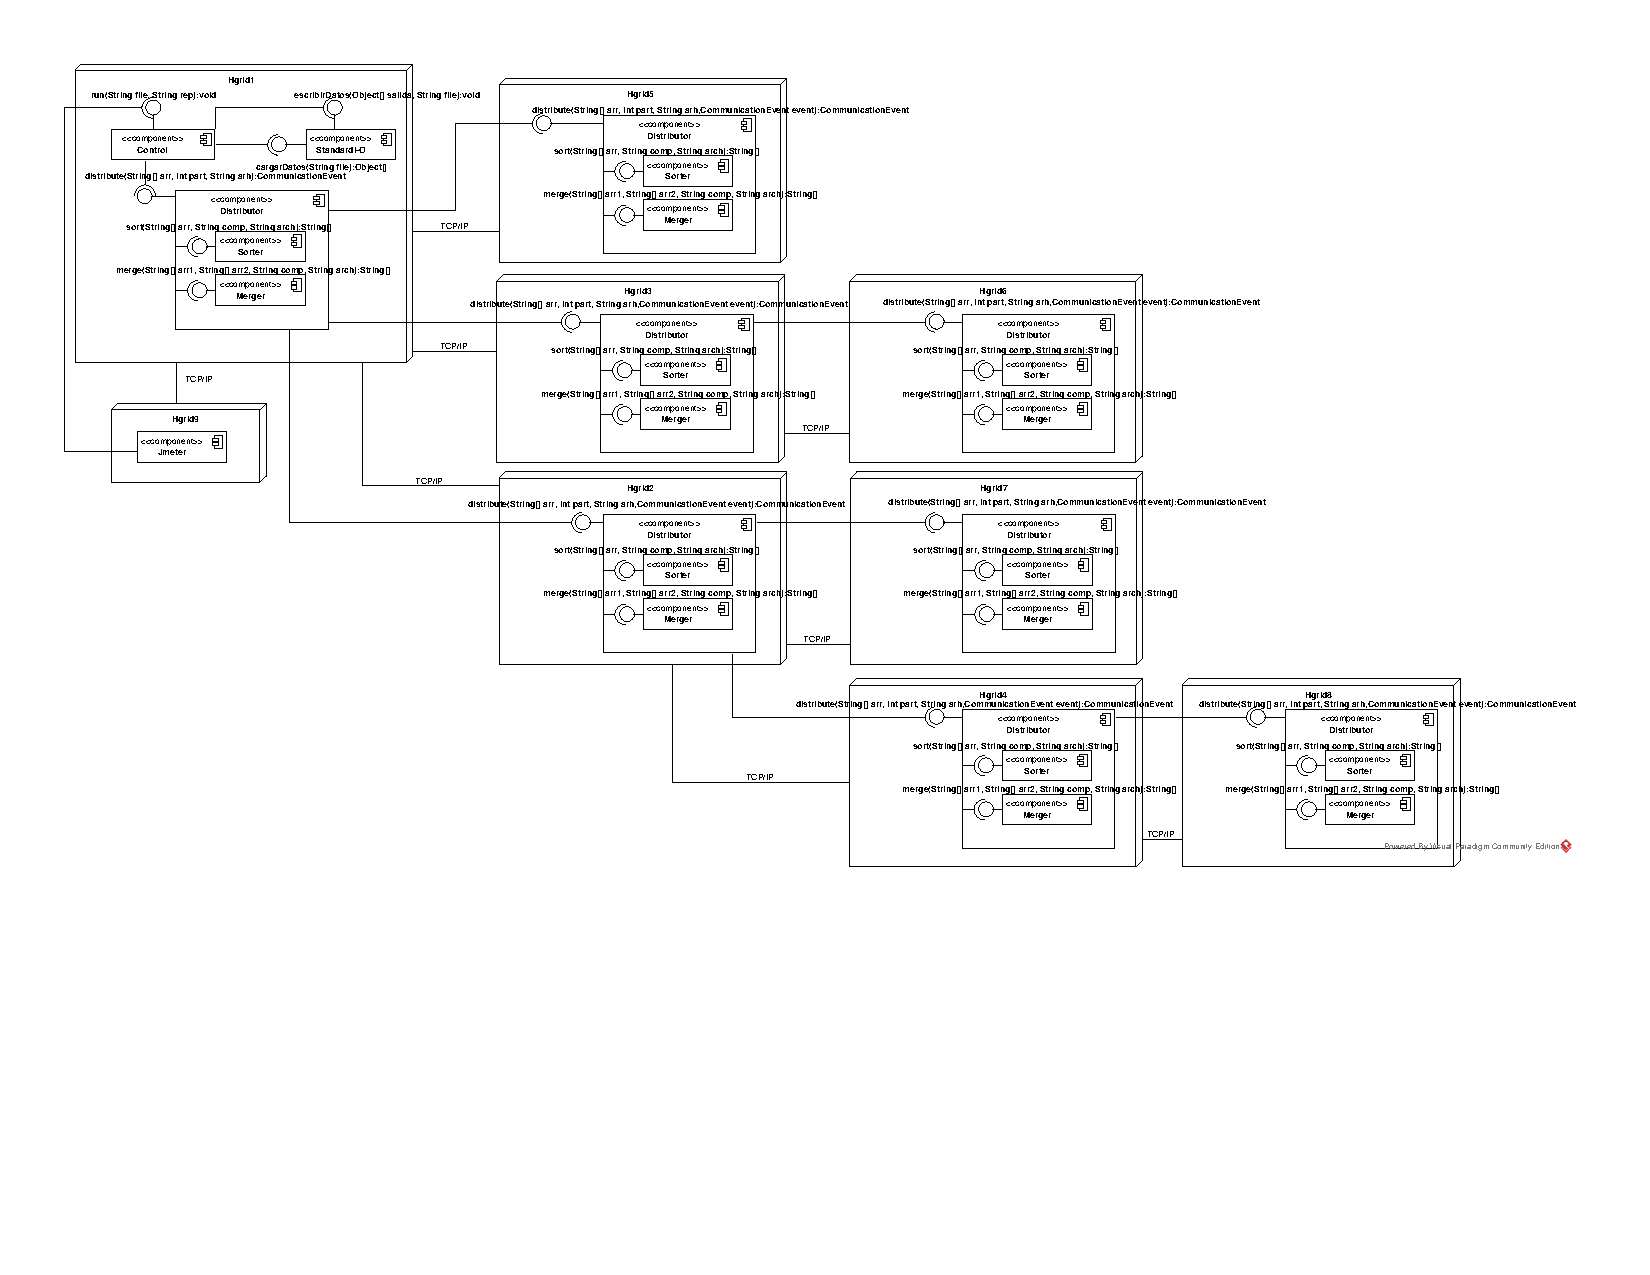
\includegraphics[trim=2cm 6cm 1cm 1cm]{fig/JCMunozDiagrams.pdf}
		\caption{Deployment Diagram - Sorting Strategy}
		\label{fig:diagramJCMunoz}
	\end{figure}	
\end{landscape}

\begin{figure}
	\centering
	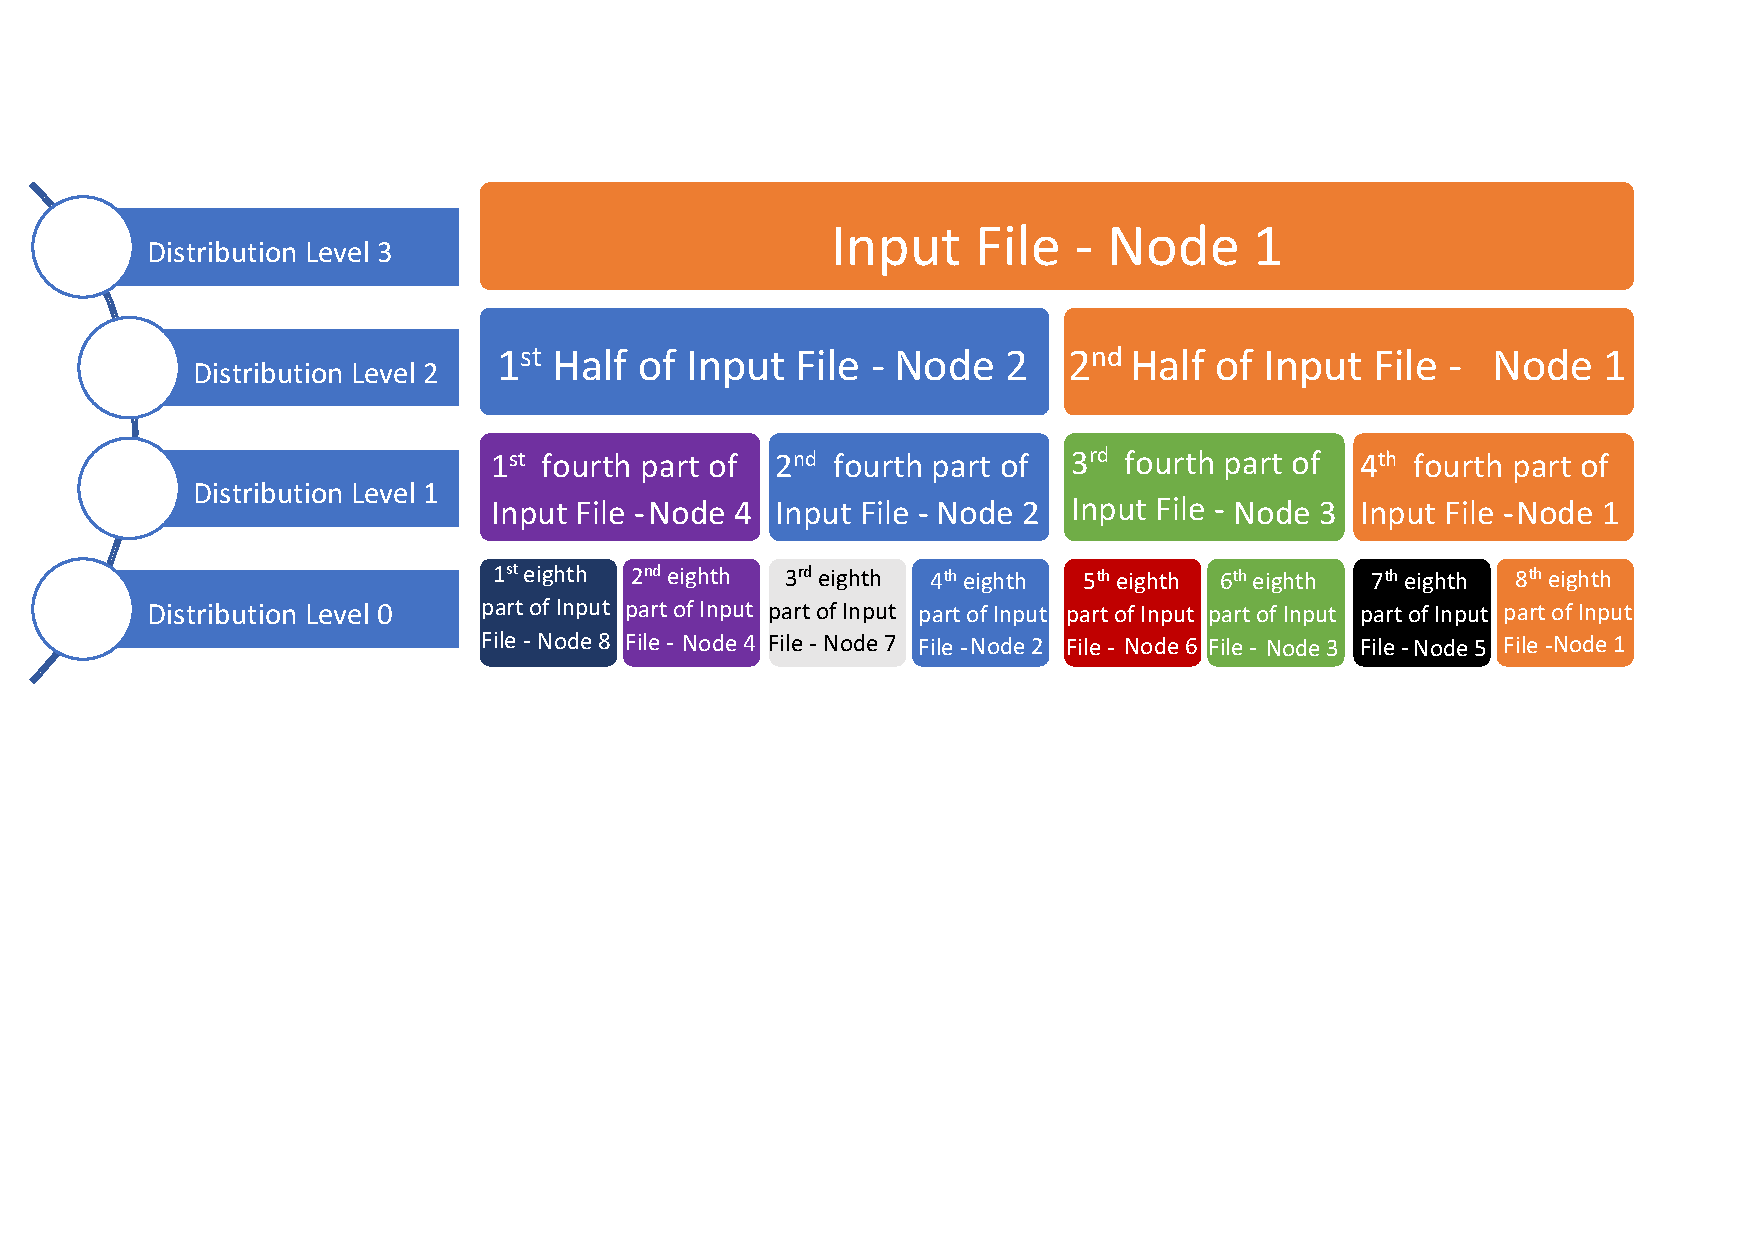
\includegraphics[trim=0cm 8cm 1cm 3cm, scale=0.6]{fig/FileProccess.pdf}
	\caption{File Distribution Process}
	\label{fig:fileProcess}
\end{figure}

\section{Selection of Specific Values of Domain-Specific Design Patterns according to the Case of Study}
\label{sec:selectdesignpatterns}

Not all domain specific performance design patterns are applicable to any problem. Therefore, to achieve the goal of this project we selected domain-specific design patterns to applying our experiments and present a justification of them as exemplars for improving software performance. Our objective is to observe how the selected patterns influence system performance.

\subsection{Applicability of the Domain Specific Design Patterns to the Sorting Problem}

\begin{itemize}
	
	\item Leader / Followers : This pattern is focused on achieving high-performance through multi-threading applications. It processes multiple types of events or service requests concurrently using independents threads (each thread works asynchronously with others). This pattern can be adapted to a distributed software configuration to exploit its benefits. In this thesis we want to leverage this pattern in a distributed environment, therefore we adapt the pattern as follows: (i) the input file to sort is divided in chunks and each chunk is translated as a sorting request, (ii) chunks of the file that must be sorted are stored in an queue to avoid missing data, and (iii) a manager must be implemented being it responsible to send a chunk from the queue to the current leader, (iv) before processing a request, each leader selects a new leader.
	
	\item Half-Synchronous / Half-Asynchronous : This pattern describes in its context two main parts, one asynchronous and one synchronous. The asynchronous part proposes to implement a queue to receive asynchronous requests. The synchronous part proposes to process a task since it starts until its ends.  This pattern is not applicable to the sorting problem because it does not involve asynchronous requests during the sorting process, so,  we would work only with the synchronous part of the process where we process one file at a time. If we want to adapt this pattern we would consume resources unnecessarily due to asynchronism proposed by this pattern. We would propose that in the same way that Leader / Followers was adapted, this pattern could be adapted, however, it implements its own queue to receive the asynchronous requests, thus, increasing latency. Therefore, we discarded it..
	
	\item Master / Workers : This pattern does not consider shared data, it only considers independent tasks. So, it is not possible to exploit this pattern in a distributed environment for the sorting problem, because not all processing nodes are leveraged if the processed file is not shared. However, one of its variants (Separable Dependencies) could be selected because of that variant considers shared data.
	
	\subitem Separable Dependencies Variant : This pattern can be applied to the sorting problem. 
	
	\subitem Geometric Decomposition Variant : This pattern is a variation of Master/Workers. This pattern considers not only independent tasks but also the shared data. To share data, this pattern proposes to divide data into chunks that interact between each other. However, to sort a chunk of a file it is not necessary to have information of other chunks of the file. This means that there is no interaction between data chunks sorters. In the merge phase, chunks could be exploited, however, it will imply to make more than one merge phase. If the sorting case is implemented using more than one merge phase, it can lose performance. That is why this pattern is not exploitable in the sorting case.
	
	\item ThreadPool : This pattern is used by other patterns such as leader / Followers. Thus, its applicability is analyzed in them.
	
	\item Fork / Join : This pattern is applicable because it proposes a way to leverage all available processing units. Since Java version 1.7, it includes an implementation of this pattern. That is the reason why we decided to implement this pattern in two levels. (i) each node implements the Java concurrent library to leverage this pattern in a parallel environment and (ii) this pattern is generalized in a distributed environment.
	
	\item Producer-Consumer : This pattern is applicable to the sorting problem.
	
	\item Random Access Parser : This pattern is applicable to improve XML files processing, thus, this pattern is not applicable in the sorting problem.
	
	\item Map-Reduce : This pattern can be applied to the sorting problem.
	
	\item Sender Released : This pattern is not applicable in this case of study because this pattern has a different main objective to the case of study. This pattern is focused on SOA applications communication to guarantee to deliver messages without affecting performance significantly. In our case, we only have one application (sorting case) and deliverability in the communication among services is not a critic point that justify to implement this pattern. (See section \ref{sec:SLRResults}).
	
	\item The State-Based-Pipeline : This pattern is leveraged when there are more than one processing phase. Even though in the sorting case there are two phases, sort and merge, only the sorting phase can be distributed to leverage the processing units. Because of this, this pattern is not applicable to the sorting problem.
	
	\item Sayl : This pattern proposes a way to leverage idle time of processing units according to task dependencies. However, in this case only the sorting phase can leverage processing units. Therefore it is not possible leverage idle time caused by task dependencies.
	
	\item Reactor : It works as a receptionist, it takes calls (requests) and redirect them to the corresponding addressee (i.e., an instance that can attend the request). In the sorting problem this behavior does not happen, because there is only one kind of request receptor. Therefore, this pattern is not applicable to the sorting problem. 
	
\end{itemize}

\subsection{Selection of the Domain Specific Design Patterns for our Experiments}

Considering to the previous section, we determine that there are 5 domain specific design patterns applicable to the sorting case (i) Leader/Followers, (ii) Separable dependencies, (iii) Fork/Join, (iv) Producer-Consumer, and (v) Map-Reduce. Additionally, our case of study application is based on the strategy proposed by Juan Carlos Mu\~{n}oz (JC Sorting Strategy). Because of this thesis scope we have to reduce the combination and possible values for this variable to three. First, we select the strategy proposed by Juan Carlos Mu\~{n}oz (i.e.,the JC Sorting Strategy) due to this is our base. Second, we use the base strategy to select patterns that could adapt in a better way to it, have in mind comparison among strategies, the pattern Fork/Join has a strategy very similar to ours, so, this has selected. Finally, we select a pattern with a different strategy and among the existing options we select the pattern that we consider could give us better performance, so, we select the Leader/Followers pattern.

\section{Variable Measurement and Monitoring}
\label{sec:measureandmonitor}
Measurement of variables is focused not only on uncontrollable variables in this thesis, we also measure the time of each of the phases of the sorting case of study. The sorting base strategy has five stages to measure: (i) read, (ii) data distribution, (iii) sort, (iv) merge, and (v) write. Communication time is a measurable variable, and also is part of the one stage of the strategy (implied in distribution stage). Finally, the number of available CPU cores variable is measured as the available percentage of each core of each node using the hyperic sigar Java library. However, this measure is not reported when it occurs like the another measurements, it variable needs a monitor that given a specific time pull the measure repetitively until the whole process finished. The another measurements are taken when a specific event occurs (e.g., when a specific component finishes sorting it sends a measurement), but the number of available CPU cores is always changing, therefore it needs a monitor that is constantly taking measurements (in this case, each five seconds, this value does not overload memory with measures and to keep an approximate on the CPU's behavior).

To take measurements, we use the PaSCAni runtime library developed by Miguel Jimenez \cite{6976605}. This library generates the components for a Dynamic Monitoring Infrastructure. The library makes it possible to measure all variables of interest by injecting in source code the code to send measurements to a probe that is responsible for managing (i.e., to receive and to send) measurement information. Additionally, a reporter component was also developed to request and consolidate the probe measurements information. It generates an excel file that contains all measurements taken during an experiment.

\section{Benchmark}
\label{sec:benchmark}
In this section we present a summary of the variables to be analyzed and their values.

\begin{description}
	\item [Available CPUs Cores.] This is an uncontrollable variable, so, for this variable we developed a CPU monitor that reads the CPU usage percentage every five seconds. Each one of the distributed processing nodes in LIASON laboratory has 8 cores (4 physical and 4 logical).
	\item [Available Nodes.] Because of the limited number of processing nodes available in the laboratory and the additional processing constraints introduced by the strategy or design pattern used (e.g., JC sorting strategy increases node in base two, $2^{0}=1 ; 2^{1}=2; 2^{2}=4; 2^{3}=8; 2^{4}=16$). This variable only takes five possible values to keep the experiments comparable.
	\item [Service Requests.] This variable is defined according to the selected performance factors. Latency is observed as one request at a time while throughput is observed as many requests at the same time.
	\item [Bandwidth.] Variation of this variable depends on the configuration options available in the laboratory's hardware, that is, 1 Gbps and 100 Mbps.
	\item [Distributed Memory Structure.] Each distributed memory structure (i.e., UMA, NUMA, COMA, NORMA) implies a code implementation. Given the scope of this thesis we selected only two memory structures. First, we selected NORMA, because this is one option of shared logical memory and distributed physical memory, and additionally, in this structure, unlike NUMA, each processing node is responsible for managing its own data and in the sorting case it allows us processing chunks of input data independently in each processing node. Second, we selected UMA, because it is the only one with shared logical and physical memory, therefore it can take advantage of the NAS device in the laboratory.
	
	On the one hand, implementing NORMA is based on dividing the file that needs to be sorted in equal size chunks according to each strategy or design pattern. Therefore, once processing nodes have their own chunk to sort, they do not need to share information between them. On the other hand, implementing UMA is based on assigning a set of data to be sorted by each processing node. That way, each node only accesses file data that were assigned to it. Implementing UMA uses the BufferedReader Java implementation and its skip method to read just the assigned data to each node.
	
	\item [Communication Protocol.] There are several frameworks, standards, platforms, and middleware developed to support distributed computation, and each one implies a different code implementation. Due to the scope of this thesis we selected only two middleware/framework that allowed us to use three communication protocols. 
	
	The first, selected middleware/framework is FraSCAti, which provides three kind of communication protocols, (i) Remote Method Invocation (RMI), (ii) Representational state transfer (REST), and (iii) Simple Object Access Protocol (SOAP). Currently, these protocols are the most used for distributed computation. However, we must select only two protocols due to time constraints. We selected the option of WebService communication protocol (REST or SOAP) and RMI. According to \cite{kumari2015performance} in general REST has better response times and throughput than SOAP, thus, we select REST as the WebService option.
	
	The second selected middleware/framework is ICE, according to \cite{articleIce}, Ice has the best performance when it was compared with the other options. Ice is a Remote procedure call (RPC) framework and it has its own Interface description language (IDL) named Slice. Therefore, our third selected communication protocol is RPC-Slice.
	
	\item [Communication Time.] This variable can only be monitored and measured and it depends mostly on the nature of the solution strategy used to solve the problem of interest, in this case the sorting problem.
	\item [Design Patterns.] Among variations of design patterns the first is the JC sorting strategy proposed by Juan Carlos Mu\~{n}oz, this strategy was described in section \ref{sec:sorting}. Despite of this strategy seems as an efficient way to leverage distribution in the context of the sorting problem, we think that it had an improvement opportunity. Therefore, we proposed a variation of this strategy where merge component is centralized. Given that each variation of this variable implies code implementation and we have two base strategies, we selected only two additional design pattern variations (i) Fork-Join and (ii) Leader-Followers (See section \ref{sec:selectdesignpatterns}). \\
	During Fork-Join implementation we find a library with Java fork-join implementation \cite{lea2000javae} and we decided to add a new variation using this library.
	\item [Performance Factors.] In this thesis we selected Latency and Throughput as performance factors to be measured and characterized (See section \ref{subsubsec:performanceFactors}).
	\item [File Size.] (Problem Size) This variable requires calibration experiments to define its possible values. The calibration experiment consists in measuring the time to sort  different file sizes using one and two  processing nodes until finding the minimum file size where using two processing nodes has better performance than using one processing node. To identify this minimum value we increased the file size in 200.000 lines each time and this calibration experiment is executed for all design pattern variation. We found that minimum file size for experiments is 1'800.000 lines (the minimum common file size for all design pattern variation). We propose increasing 400.000 lines at a time until reaching 9'800.000 lines to execute our experiments. The minimum file size found is the point in which distribution environment can be leveraged. Table \ref{tab:mimfileSizeEx} shows results of this calibration experiment.
\end{description}

Table \ref{tab:benchmarks} summarizes experiments variations to be performed, that is, our design for the experiments.

\begin{table}[]
	\centering
	\caption{Benchmark Consolidation}
	\label{tab:benchmarks}
	\resizebox{\textwidth}{!}{%
		\begin{tabular}{|c|c|c|c|c|}
			\hline
			\textbf{Id} & \textbf{\begin{tabular}[c]{@{}c@{}}Context\\   Variables\end{tabular}} & \textbf{Possible Values}                                                                                                                                                                                                                            & \textbf{Controllable} & \textbf{\begin{tabular}[c]{@{}c@{}}Possible\\   Variations\end{tabular}} \\ \hline
			1           & \begin{tabular}[c]{@{}c@{}}Available\\ CPU Cores\end{tabular}              & {[}1-8{]}                                                                                                                                                                                                                                           & No                    & NA                                                                        \\ \hline
			2           & \begin{tabular}[c]{@{}c@{}}Available Distributed\\ Processing Nodes\end{tabular}             & {[}1, 2, 4, 8,16{]}                                                                                                                                                                                                                                 & Yes                    & 5                                                                        \\ \hline
			3           & \begin{tabular}[c]{@{}c@{}}Service\\ Requests\end{tabular}             & \begin{tabular}[c]{@{}c@{}}1. 10 files, one file at a time for latency.\\ 2. Amount of files needed to maintain load \\ during 20 minutes for throughput.\end{tabular}                                                                                       & Yes                    & 2                                                                        \\ \hline
			4           & Bandwidth                                                              & {[}100 Mbps - 1 Gbps{]}                                                                                                                                                                                                                                   & Yes                    & 2                                                                        \\ \hline
			5           & \begin{tabular}[c]{@{}c@{}}Memory\\ Structure\end{tabular}             & UMA, NORMA                                                                                                                                                                                                                                          & Yes                    & 2                                                                        \\ \hline
			6           & \begin{tabular}[c]{@{}c@{}}Communication\\   Protocol\end{tabular}     & REST, Slice, RMI                                                                                                                                                                                                                                    & Yes                    & 3                                                                        \\ \hline
			7           & \begin{tabular}[c]{@{}c@{}}Communication\\ Time\end{tabular}           & {[}0-*{]} (Continuous)                                                                                                                                                                                                                                          & No                    & NA                                                                        \\ \hline
			8           & \begin{tabular}[c]{@{}c@{}}Design Patterns\\ and Strategies Variation\end{tabular}  & \begin{tabular}[c]{@{}c@{}}1. JC Sorting Strategy.\\     2. JC Sorting Strategy Variation \\ (separated merger).\\     3. Fork/Join Java library.\\     4. Fork/Join Java library and\\  Distributed Fork/Join.\\     5. Leader-Followers.\end{tabular} & Yes                    & 5                                                                        \\ \hline
			9           & \begin{tabular}[c]{@{}c@{}}Performance\\ Factors\end{tabular}          & Latency, Throughput                                                                                                                                                                                                                                 & Yes                    & 2                                                                        \\ \hline
			10          & File Size                                                              & \begin{tabular}[c]{@{}c@{}}From 1'800,000 To 9'800,000 \\ with increasing steps of 400,000\end{tabular}                                                                                                                                                   & Yes                    & 21                                                                       \\ \hline
		\end{tabular} %
	}
\end{table}

\section{Chapter Summary}
In this chapter, we follow step by step how we design our solution proposal. We started proposing computational experiments as a possible solution for our problem, so, we define a design of experiments applied it. However, proposing the design was not a trivial task, we first identify the involved variables in the problem. After, we define strategies of control and replication to assurance experiments' reliability. Next, we select a case of study over which we apply the domain-specific design patterns to execute different experiment configurations and based on it we could evaluate the quantitative impact that patterns for performance have on the system, in this case, we selected sorting as our study case. Due to the thesis scope, we can not execute experiments about all domain-specific design patterns that could be applied to our study case, so, we had to select which we consider as the more relevant according to their impact over our problem and their applicability over our study case. Later, we define how we take the measurements and how we monitor the studied variables. Finally, we resume all decisions that we toke in the benchmark section where we present the design of the consolidate experiment.

	% =========================================================================
	\chapter{Experiments Execution}
	\label{cha:expExecution}
	\section{Configuration and Control of Experiments}
\label{sec:confandControl}
Software experiments that do not require interacting directly with humans (e.g., through graphic user interfaces (GUI) or Human–computer interaction software (HCI)) are not strongly influenced by human factors (e.g., personality, preferences, human environment, education, age, culture, among others). However, there are related variables that must be configured to ensure that they won't affect the experiments results. These configurations are realized to guarantee the experiments reliability and it is also known as calibration. Additionally, they are accompanied by experiments rehearsals. It is important to guarantee that there are no unidentified variables that affect the results of the experiments before starting the experiments execution. In this case, these variables refer to the configuration of experiments, including, the Precision Time Protocol (PTP), the Java version and the Java Virtual Machine (JVM) configuration, the software deployment configuration, the operating system, and the hardware configuration. Some of these variables were described in section \ref{sec:contextVariablesSearch} showing their importance on systems performance. However, in our case, we do not vary their values to determine how they affect performance. We only select one configurable value to each one to control how they affect system performance with these definitions and values, we performed pilot experiments to calibrate and tune the chosen values that allow us to guarantee that these variables configuration and the unidentified variables do not affect the experiments. 

\subsection{Hardware Configuration}
Experiments were executed out in the LIASOn laboratory of the Universidad Icesi. This laboratory has 18 computers that are used as processing nodes, a Network Attached Storage (NAS) that allows information to be shared among processing nodes, and its own private network, through a 10 Gbps switch with 24 ports. Table \ref {tab:hardware_config} summarizes characteristics of the device types. 

\begin{table}[]
	\centering
	\caption{Hardware Configuration}
	\label{tab:hardware_config}
	 \resizebox{\textwidth}{!}{%
	\begin{tabular}{|c|c|c|c|c|c|}
		\hline
		\textbf{DEVICE}                                                               & \textbf{NAME}                                                              & \textbf{PROCESSOR}                                                              & \textbf{\begin{tabular}[c]{@{}c@{}}OPERATING\\ SYSTEM\end{tabular}}                       & \textbf{MEMORY}       & \textbf{HDD}       \\ \hline
		\begin{tabular}[c]{@{}c@{}}Processing \\ Nodes (18) \end{tabular}                                                                            & \begin{tabular}[c]{@{}c@{}}DELL \\ OPTIPLEX 7010\end{tabular}              & \begin{tabular}[c]{@{}c@{}}Intel Core i7 - 3770 \\ @3.40Ghz (4 physical cores)\end{tabular}        & \begin{tabular}[c]{@{}c@{}}Fedora 21 \\ 64 bits\end{tabular}                              & 16 GB                 & 320 GB             \\ \hline
		\multicolumn{6}{|c|}{}                                                                                                                                                                                                                                                                                                                                                                \\ \hline
		\begin{tabular}[c]{@{}c@{}}Network\\   Attached \\ Storage (NAS) (1)\end{tabular} & \begin{tabular}[c]{@{}c@{}}Dell Power \\ Vault NX400\end{tabular}          & \begin{tabular}[c]{@{}c@{}}Intel ® Xeon\\   ® E5-2403 \\ Quad Core\end{tabular} & \begin{tabular}[c]{@{}c@{}}Microsoft Windows\\     Storage Server \\ 2012 R2\end{tabular} & 18 GB                 & 4 TB               \\ \hline
		\multicolumn{2}{|c|}{}                                                                                                                                     & \multicolumn{2}{c|}{\textbf{SUPPORTED TRANSMISSION RATE}}                                                                                                                            & \multicolumn{2}{c|}{\textbf{PORTS}} \\ \hline
		Switch (1)                                                                        & \begin{tabular}[c]{@{}c@{}}Dell Networking\\     N4000 Series\end{tabular} & \multicolumn{2}{c|}{10/100/1000/10000  (Mb/s)}                                                                                                                              & \multicolumn{2}{c|}{24}                    \\ \hline
	\end{tabular}%
}
\end{table}

\subsection{Operating System Configuration}
As we mentioned in section \ref{sec:contextVariablesSearch}, the operating system can affect the system performance given that it is responsible to manage hardware resources through daemon processes and user processes and provide services to applications to access or use the hardware resources. In our experiments, all processing nodes have Fedora 21 operating system (64 bits). Its daemon processes serves main functions, not all of them required for executing the experiments, thus, we  analyze which of these processes are needed during our experiments execution and we developed a script to shutdown unnecessary processes that the operating system might start. The objective of this script is to minimize the possibility that one of these processes may affect the experiments using resources for other tasks outside of our experiments. To develop the script, we explored one by one each of them and determined if our application or operating system required this service or process. (The script is presented in Appendix A - section \ref{sec:appendA}).

\subsection{Precision Time Protocol (PTP)}
Precision Time Protocol (PTP) is a software implementation of the IEEE standard 1588 for Linux. In this thesis, this protocol has a special role because for taking measurements in distributed environments requires synchronization among processing nodes. For example, when we measure communication time, this time has to be collected in two different nodes (sender and receiver). The communication time is calculated as the difference between the instant the message is received (time in milliseconds) minus the instant the message is sent (time in milliseconds). If nodes are not synchronized, this measurement is not accurate. This protocol allows a precision in nanoseconds, and measurements are taken in milliseconds, so it fulfills the measurement requirements. 


\subsection{Other Software and their Configurations}
Other variables that also must be configured are the instrumentation variables. These are the ones that are used to execute the experiments, for example,  middle-ware and support software. These variables can affect the experiments results through their own values and procedures of configuration, or the used version, because depending on them each application can change the way to manage its resources, and therefore they affect the system performance. The following are the software versions and their configuration used during experiments.

\begin{description}
	\item [FraSCAti:] This software is used to support SCA component implementation. We use Frascati version 1.4 because it was the most stable version available.
	\item [Ice:] This software is used to support the communication between distributed components. We use Ice version 3.5.
	\item [Java:] All code of the applications to execute the experiments was implemented in java. We use Java version 1.6 Update 23 because it is the most compatible with FraSCAti.
	\item [Tomcat:] This is used as a server application facade when we use Ice because the basic version of Ice does not manage REST requests. We use Tomcat version 8.
	\item [Jmeter:] This is used to simulate user requests. We used Jmeter version 2.13.
	\item [RabbitMQ:] This is used by PaSCAni library to send and take measurements to probes.  We used RabbitMQ version 3.6 (Configuration is presented in section \ref{sec:appendB} - Appendix B).
	\item [Java Virtual Machine (JVM) Configuration:] Java Virtual Machine configuration can affect experiments. However, we only focus on maximum and minimum memory configuration. Memory size can affect the experiments directly given the size of the files that have to be sorted. We configured the JVM memory to 6 GB (Configuration is presented in section \ref{sec:appendC} - Appendix C).
	
\end{description}


\section{Software Deployment Configuration}
Amelia is a library developed by Miguel Jimenez \cite{AmeliaMiguelJimenez} to automate the deployment of distributed component-based software. Using this library, we implemented classes to automate the execution of experiment designed in chapter \ref{cha:experimentDesign}. In the next sections, we present the deployment diagrams for the sorting software for all design pattern and strategies variation that we used as architectural guides to implement the required classes, as their deployment specification.

\subsubsection{JC Sorting Strategy}
\label{subsubsec:ameliaOriginalStrategy}
This strategy consists in splitting the input data recursively to halves while there are available processing nodes. For example, for 4 available nodes configuration (cf. figure \ref{fig:diagramJCMunozOriStr})  and a file size of 1'600.000 lines. First node splits the input data to half (800.000 lines), it keeps one half to process and sends the other half to its son, in the next higher hierarchical level. Its son splits input data again (400.000), and  sends to its son one half, and processes the other half. To continue with first node, it splits data again (400.000) and it sends to its other son one half, and it processes the remaining.

Figure \ref{fig:diagramJCMunozOriStr} shows the deployment diagram used to develop the amelia deployment automation classes. Almost all controllable variable combinations generate a new Amelia deployment classes, except the File Size and the Bandwidth variables. For these two variables, the amelia deployment classes can be reused using parameters. However, deployment diagrams only vary according to available processing nodes variable. This variable can take the next values: 1, 2, 4, 8, and 16 as established in the experiment design (cf. section \ref{sec:benchmark}). The presented diagram corresponds to the 8 nodes configuration. This diagram can be used to visualize all other configurations. 

To visualize the 2 nodes configuration, the processing nodes Hgrid1 and Hgrid5 are used to sort the input file. The 4 nodes configuration, Hgrid3 and Hgrid6 are added as processing nodes. To visualize the 16 nodes configuration the idea is to connect Hgrid1 with an additional node, and this new node has the same hierarchical structure of Hgrid1 in 8 nodes configuration (i.e., recursively). 

The Hgrid9 is not a processing node. It has components needed to take measurements and make reports. Hgrid17 is neither a processing node: it has components needed to automate experiments and the RabbitMq Server to support the measurements message passing. Nodes Hgrid9 and Hgrid17 remains the same through all experiments configuration.


\begin{landscape}
	\begin{figure}[p!]
		\centering
		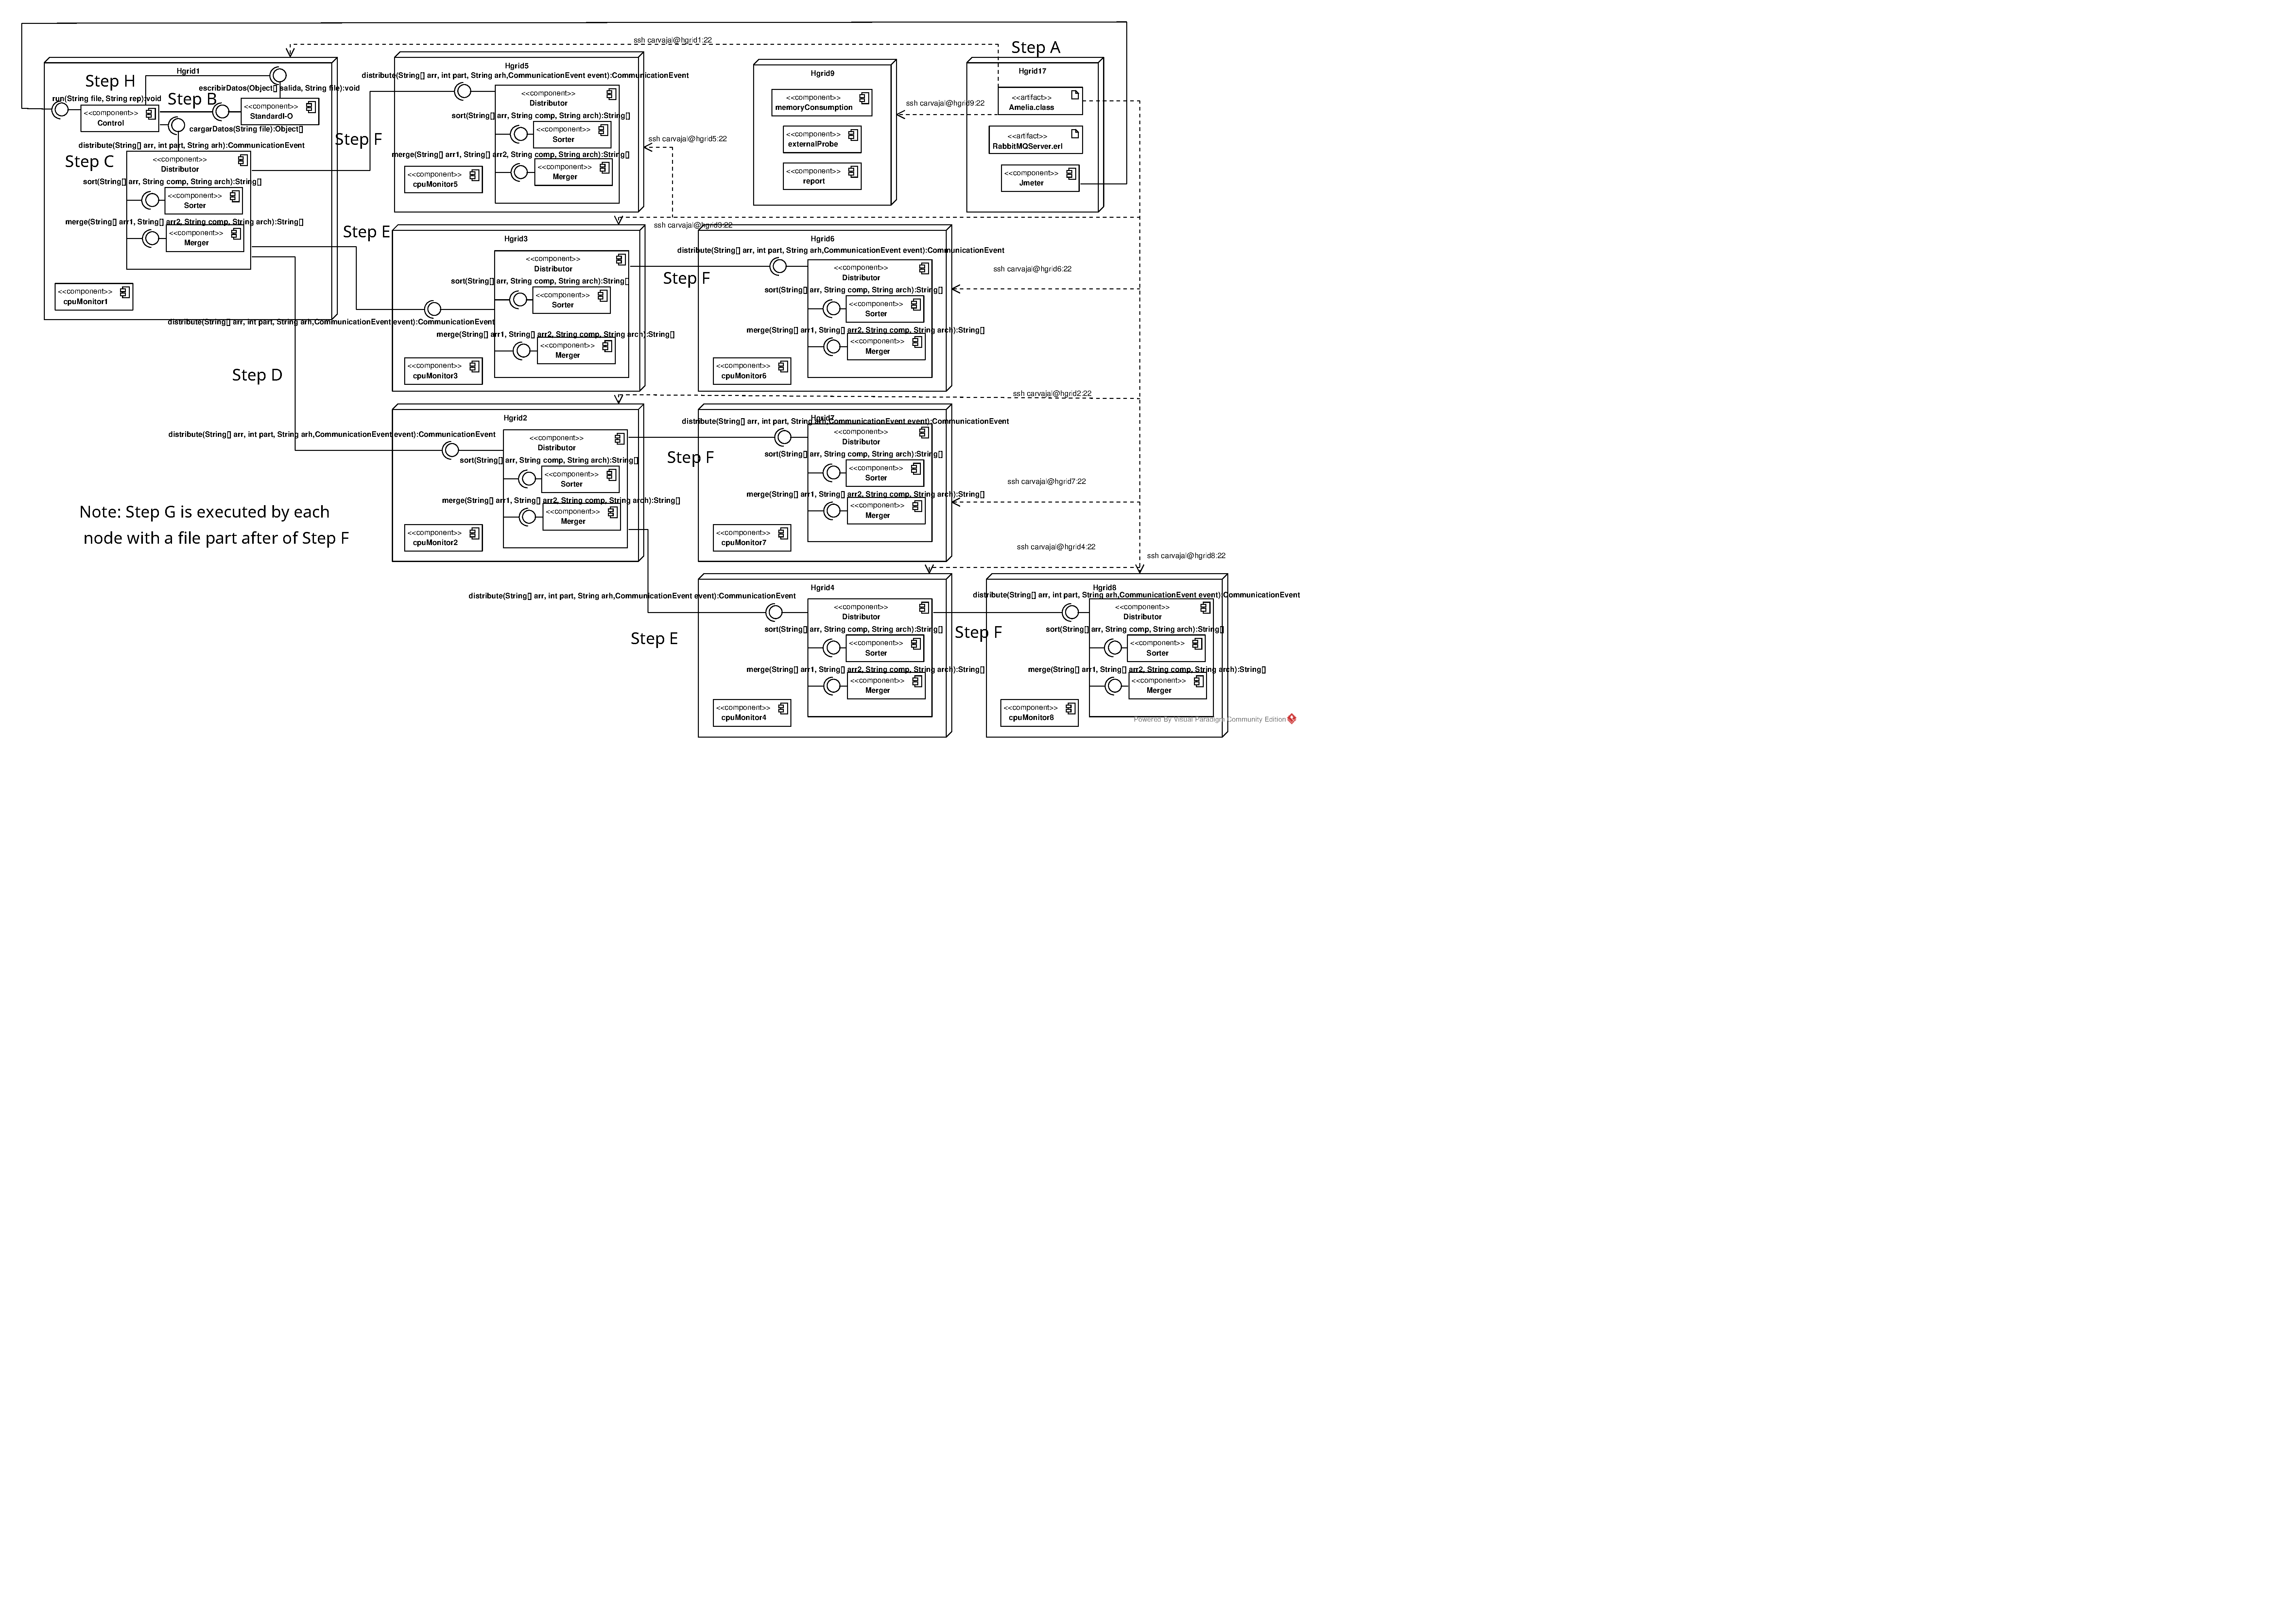
\includegraphics[trim=4cm 45cm -4cm 2cm, scale=0.4]{fig/JCMunozOriginalStrategy.pdf}
		\caption{Amelia - Deployment Diagram - The JC Sorting Strategy}
		\label{fig:diagramJCMunozOriStr}
	\end{figure}
	
\end{landscape}

The behavior of the JC Sorting Strategy is described next:\\

\begin{description}
	\item [Step A] The Jmeter component of processing node Hgrid17 starts processing when it calls the run method of the control component (processing node Hgrid1).
	\item [Step B] The control component sends to the StandardI-O component a read request to load the input file.
	\item [Step C] The control component sends to the Distributor component in Hgrid1 a distribute request with the whole input file as parameter.
	\item [Step D] The Distributor component of Hgrid1 sends to the Distributor component in Hgrid2 a distribute request with the half of the input file.
	\item [Step E] In this step two requests are sent in parallel. The Distributor component of Hgrid1 sends to the Distributor component in Hgrid3 a distribute request with a 1/4 of the input file and the Distributor component of Hgrid2 sends to the Distributor component in Hgrid4 a distribute request with a 1/4 of the input file.
	\item [Step F] In this step four request are sent in parallel. (i) The Distributor component of Hgrid1 sends to the Distributor component in Hgrid5 a distribute request with a 1/8 of the input file; (ii) the Distributor component of Hgrid2 sends to the Distributor component in Hgrid7 a distribute request with a 1/8 of the input file; (iii) the Distributor component of Hgrid4 sends to the Distributor component in Hgrid8 a distribute request with a 1/8 of the input file; and (iv) the Distributor component of Hgrid3 sends to the Distributor component in Hgrid6 a distribute request with a 1/8 of the input file.
	\item [Step G] All processing nodes sort their file part and return each sorted file part to their own father processing node, which merges the file parts.
	\item [Step H] The control component receives the whole sorted file and it sends a write request to the StandardI-O component.
\end{description}


\subsubsection{Variant of the JC Sorting Strategy - Separation of Merge Component}
This variant is illustrated in Fig. \ref{fig:diagramJCMunozMergerSeparated}. It applies the same configuration used in the previous diagram (cf. Figure \ref{fig:diagramJCMunozOriStr}), with the only difference that there is only one merge component. The merge component is located in the processing node Hgrid1. We proposed this difference for the merge solution must have complexity of O(n) and it can be incremented because of amount the recursive merge stages, therefore, we calculate that the performance can be improved if there is only one merge phase because in the JC sorting strategy there are more than one merge of the same data.

\begin{landscape}
	\begin{figure}[p!]
		\centering
		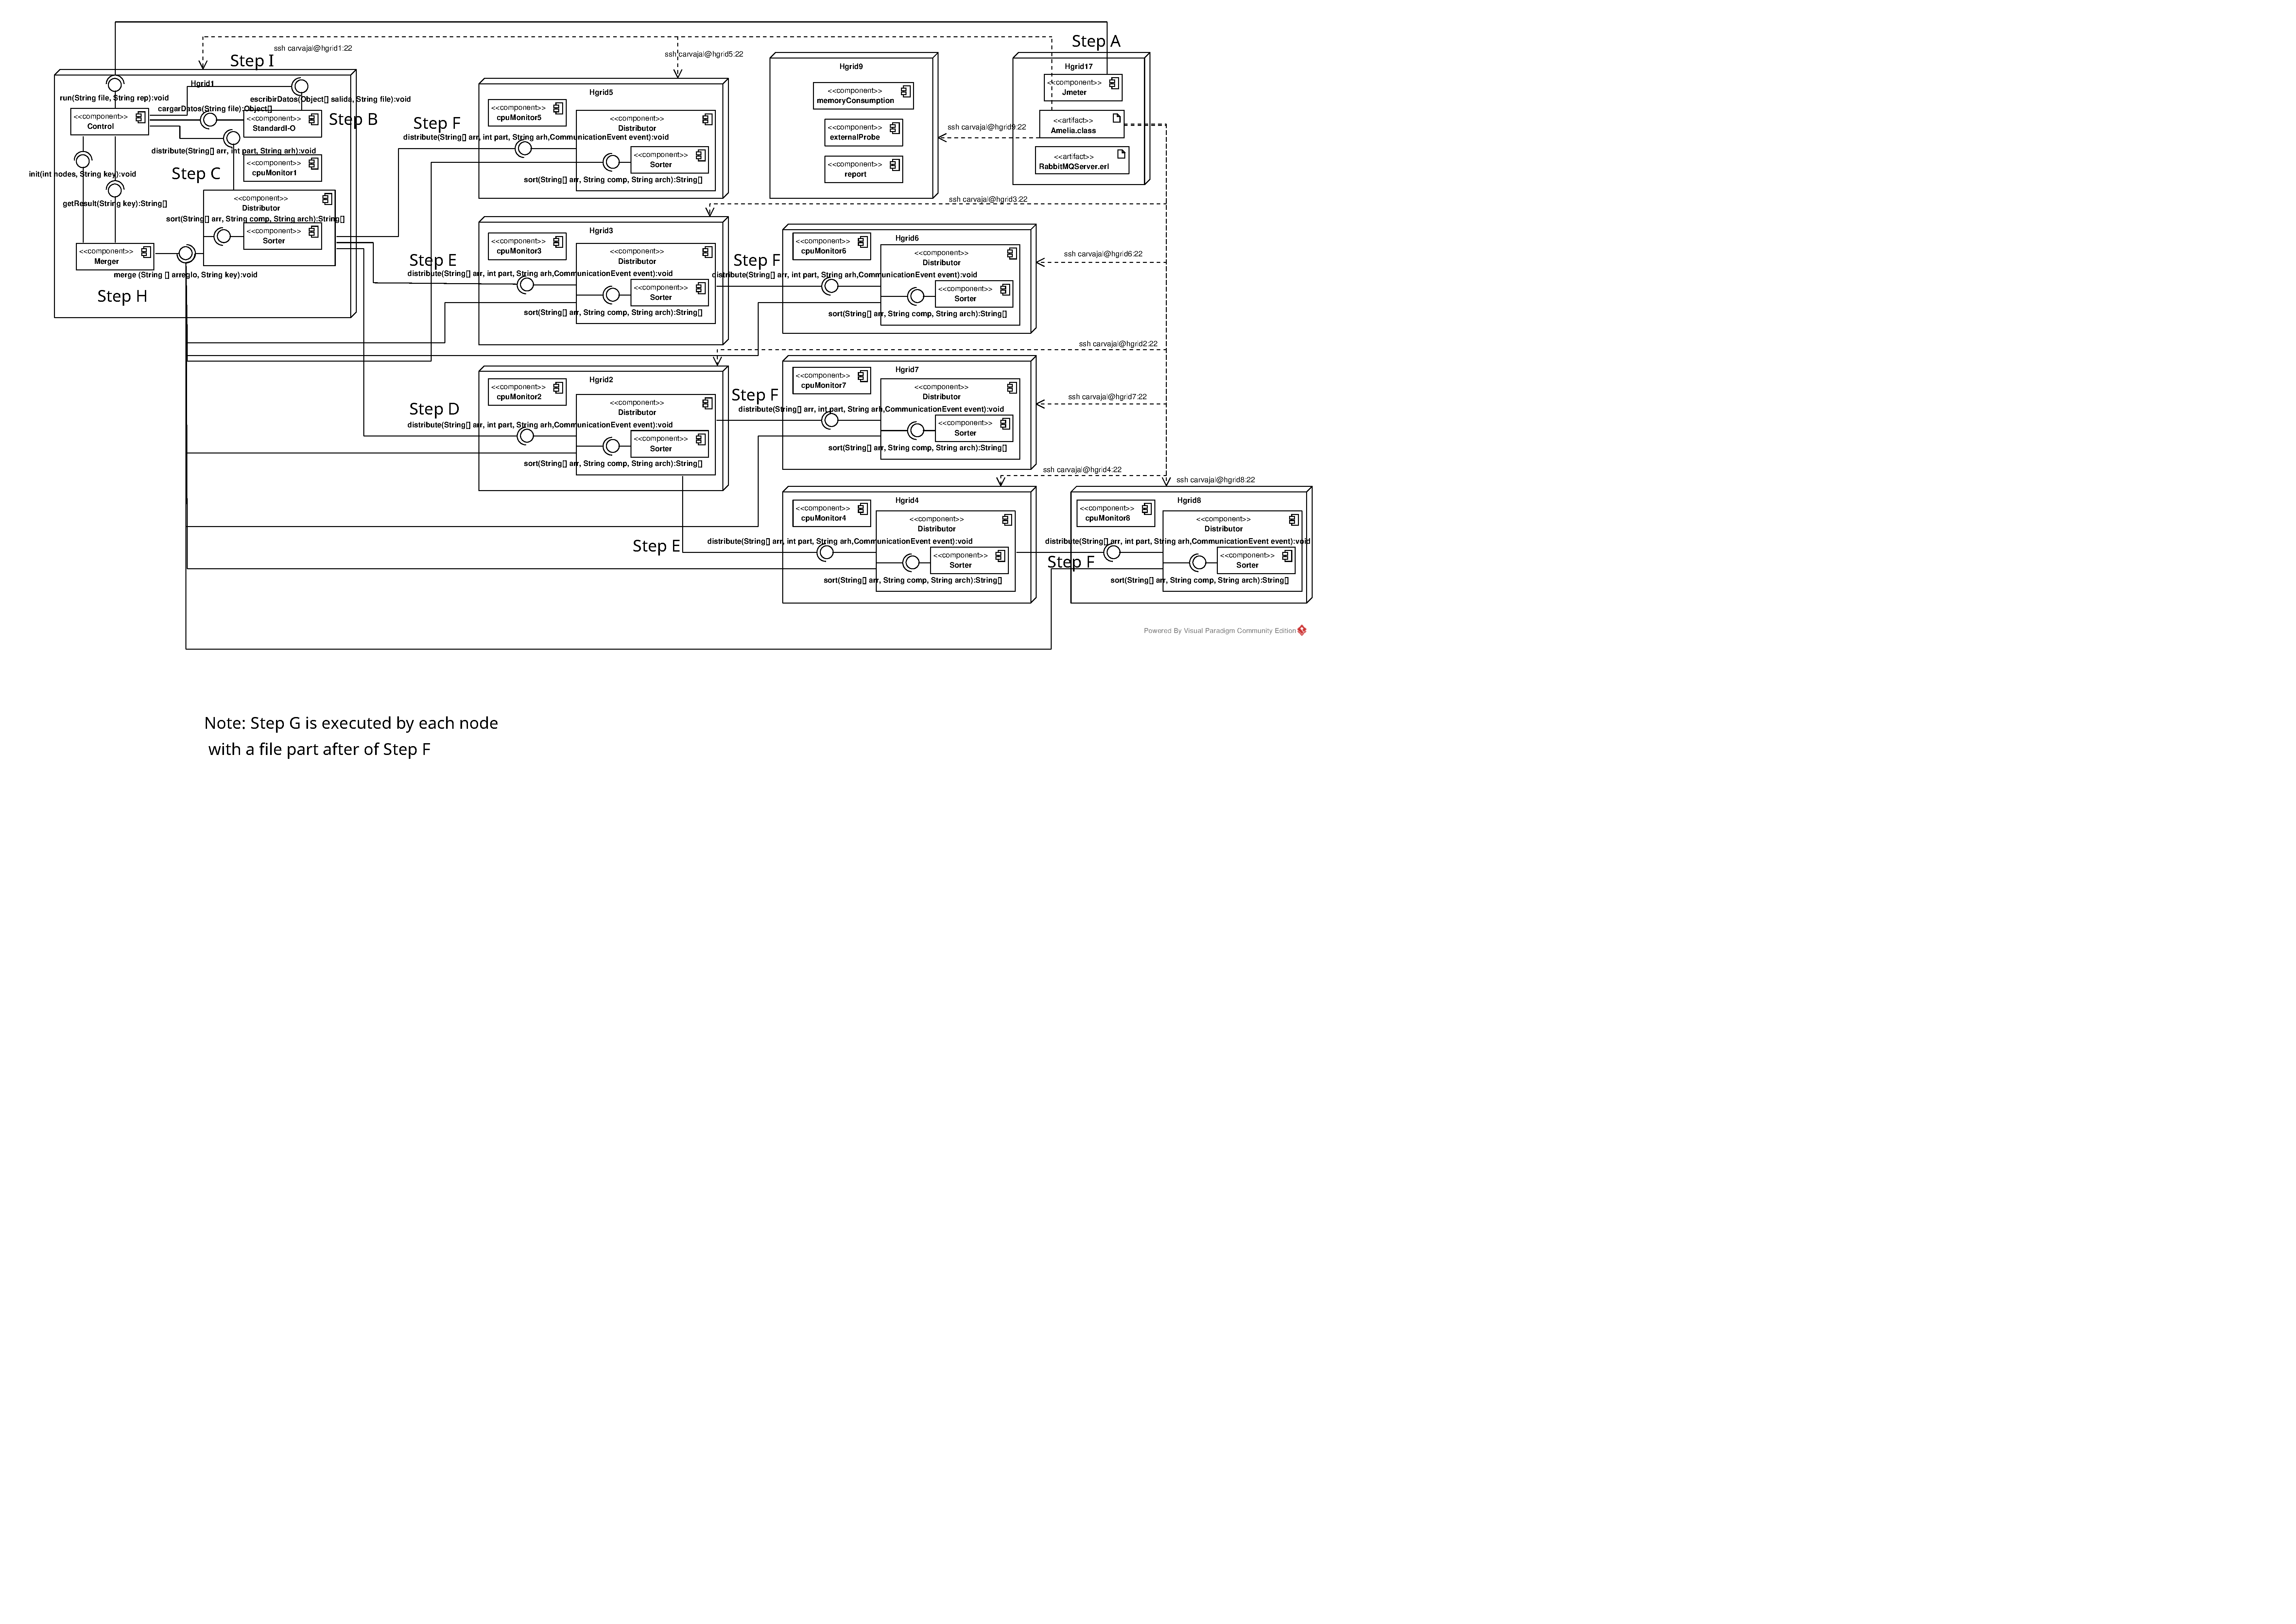
\includegraphics[trim=6cm 45cm -6cm 2cm, scale=0.4]{fig/JCMunozMergerSeparated.pdf}
		\caption{Amelia - Deployment Diagram - Variant of the JC Sorting Strategy - Separation of Merge Component}
		\label{fig:diagramJCMunozMergerSeparated}
	\end{figure}
	
\end{landscape}

The behavior of the Variant of the JC Sorting Strategy is described next:

\begin{description}
	\item [Step A] The Jmeter component of the processing node Hgrid17 starts processing when it calls the run method of the control component (processing node Hgrid1).
	\item [Step B] The control component sends to the StandardI-O component a read request to load the input file.
	\item [Step C] The control component sends to the Distributor component in Hgrid1 a distribute request with the whole input file as parameter.
	\item [Step D] In this step two request are sent in parallel. The Distributor component of Hgrid1 sends to the Distributor component in Hgrid2 a distribute request with the half of the input file and the control component initializes the merger component.
	\item [Step E] In this step three request are sent in parallel. (i) The Distributor component of Hgrid1 sends to the Distributor component in Hgrid3 a distribute request with a 1/4 of the input file; (ii) the Distributor component of Hgrid2 sends to the Distributor component in Hgrid4 a distribute request with a 1/4 of the input file; and (iii) the control component sends to the merger component a request to get the whole sorted file when all file parts will be merged.
	\item [Step F] In this step four request are sent in parallel. (i) The Distributor component of Hgrid1 sends to the Distributor component in Hgrid5 a distribute request with a 1/8 of the input file; (ii) the Distributor component of Hgrid2 sends to the Distributor component in Hgrid7 a distribute request with a 1/8 of the input file; (iii) the Distributor component of Hgrid4 sends to the Distributor component in Hgrid8 a distribute request with a 1/8 of the input file; and (iv) the Distributor component of Hgrid3 sends to the Distributor component in Hgrid6 a distribute request with a 1/8 of the input file.
	\item [Step G] All processing nodes sort their file part and send a merger request to the merger component with their own sorted file part.
	\item [Step H] The merger component receives all sorted file parts, and merges them and answers to the control component the request realized in Step E.
	\item [Step I] The control component receives the whole sorted file and it sends a write request to the StandardI-O component.
\end{description}

\subsubsection{Fork/Join Java library}
This variant uses the same deployment diagram used for the previous variant. However, it differs to the previous because it implements Java Fork-Join library in each node to process its own file chunk.

\subsubsection{Fork-Join Design Pattern}
The JC sorting strategy introduces latency given its hierarchical structure. By applying the Fork/Join pattern we can avoid this added latency. To implement this design pattern in a distributed deployment we need to answer two questions:
 \begin{itemize}
 	\item Which is the minimum chunk size worth if distributing the computations?
 	\item How many available nodes (children) should have each processing node to distribute?
 \end{itemize}
  
  The first question focuses on cases where distribution is not cost effective because distribution implies performance loss due to latency addition. The second question is focused on managing the processing nodes. The Fork/Join Java library leaves this task to the operating system through CPU core assignment. However, in a distributed deployment we must decide how processing nodes are assigned. We identify two options (i) only one node can execute forks and it has all available processing nodes associated to it; and (ii) all nodes can execute forks, but each one has a limited amount of processing nodes associated to it. When this amount is reached, if there appear a new available node it is assigned to next level of processing nodes (children of children, that is, grandchildren). For example, assuming that the limited amount is three nodes, if the first node has three associated nodes and there is a new available node, this node would be associated with any of the three children of the first node.

We will analyze the answer to the first question in the next section (cf. section \ref{sec:prepExperiments}) because in this section we will realize tests through preparatory experiments to decide which will be the minimum chunk size.
% results of experiments consolidated in table \ref{tab:mimfileSizeEx}. We decide take as minimum size to fork 400.000 lines because it is possible to observe that 200.000 lines and 600.000 lines can leverage distribution, therefore we calculate average between these values. Additionally we can observe that difference between 1 and 2 nodes for 400.000 lines is small.

To answer the second question, where we need to define how many children nodes can have each node, we try to select a behavior similar to the used in the JC sorting strategy to increase comparability. According to this, the second option (ii) exposed before, where all nodes will have the capacity of executing forks, is more appropriate. In this option we can distribute in a similar way that the JC sorting strategy, but the hierarchical structure will be more homogeneous, besides avoiding performance loss added by the added latency in the hierarchy when more nodes are added. The maximum amount of processing nodes associated to each node was defined in 3 because it can support the maximum amount of processing nodes defined for our experiments (16).

Figure \ref{fig:diagramJCMunozDistributedFJ} shows the deployment diagram of this configuration for 8 nodes.

The Fork-Join Design Pattern behavior is described as follows:

\begin{description}
	\item [Step A] The Jmeter component of the processing node Hgrid17 starts processing when it calls the run method of the control component (processing node Hgrid1).
	\item [Step B] The control component sends to the StandardI-O component a read request to load the input file.
	\item [Step C] The control component sends to the Distributor component in Hgrid1 a distribute request with the whole input file as parameter.
	\item [Step D] In this step the merger component is initialized and the first level of distributors are called in parallel. The Distributor component of Hgrid1 sends to the Distributor components in Hgrid2, Hgrid3 and Hgrid4 a distribute request with a 1/4 of the input file.
	\item [Step E] In this step some requests are sent in parallel: (i) The Distributor components in Hgrid2, Hgrid3 and Hgrid4 send to their own children Distributor components in Hgrid6, Hgrid7, Hgrid10 and Hgrid13 a distribute request with a 1/8 of the input file; (ii) the Distributor component in Hgrid1 starts to sort its file part. First, it divides its file part in more little chunks (these chunks depend on the CPU amount of each node, in our case each node divides its file part into 8 parts) to apply the Fork/Join Java library and to have work if any of its children will finish processing before and so help it. When this component finishes to process each file part, it sends a merger request to the merger component with its own sorted file parts; and (iii) the control component sends to the merger component a request to get the whole sorted file when all file parts will be merged.
	\item [Step F] In this step all Distributor components start to sort their file part, in the same way that the Distributor component in Hgrid1 did in the step E. When any of the sorter components finishes their work, it verifies if it can help its father node or the work have been finished.
	\item [Step G] The merger component receives all sorted file parts, it merges the whole sorted file and answers to the control component the request realized in Step E.
	\item [Step H] The control component receives the whole sorted file and it sends a write request to the StandardI-O component.
\end{description}

\begin{landscape}
	\begin{figure}[p!]
		\centering
		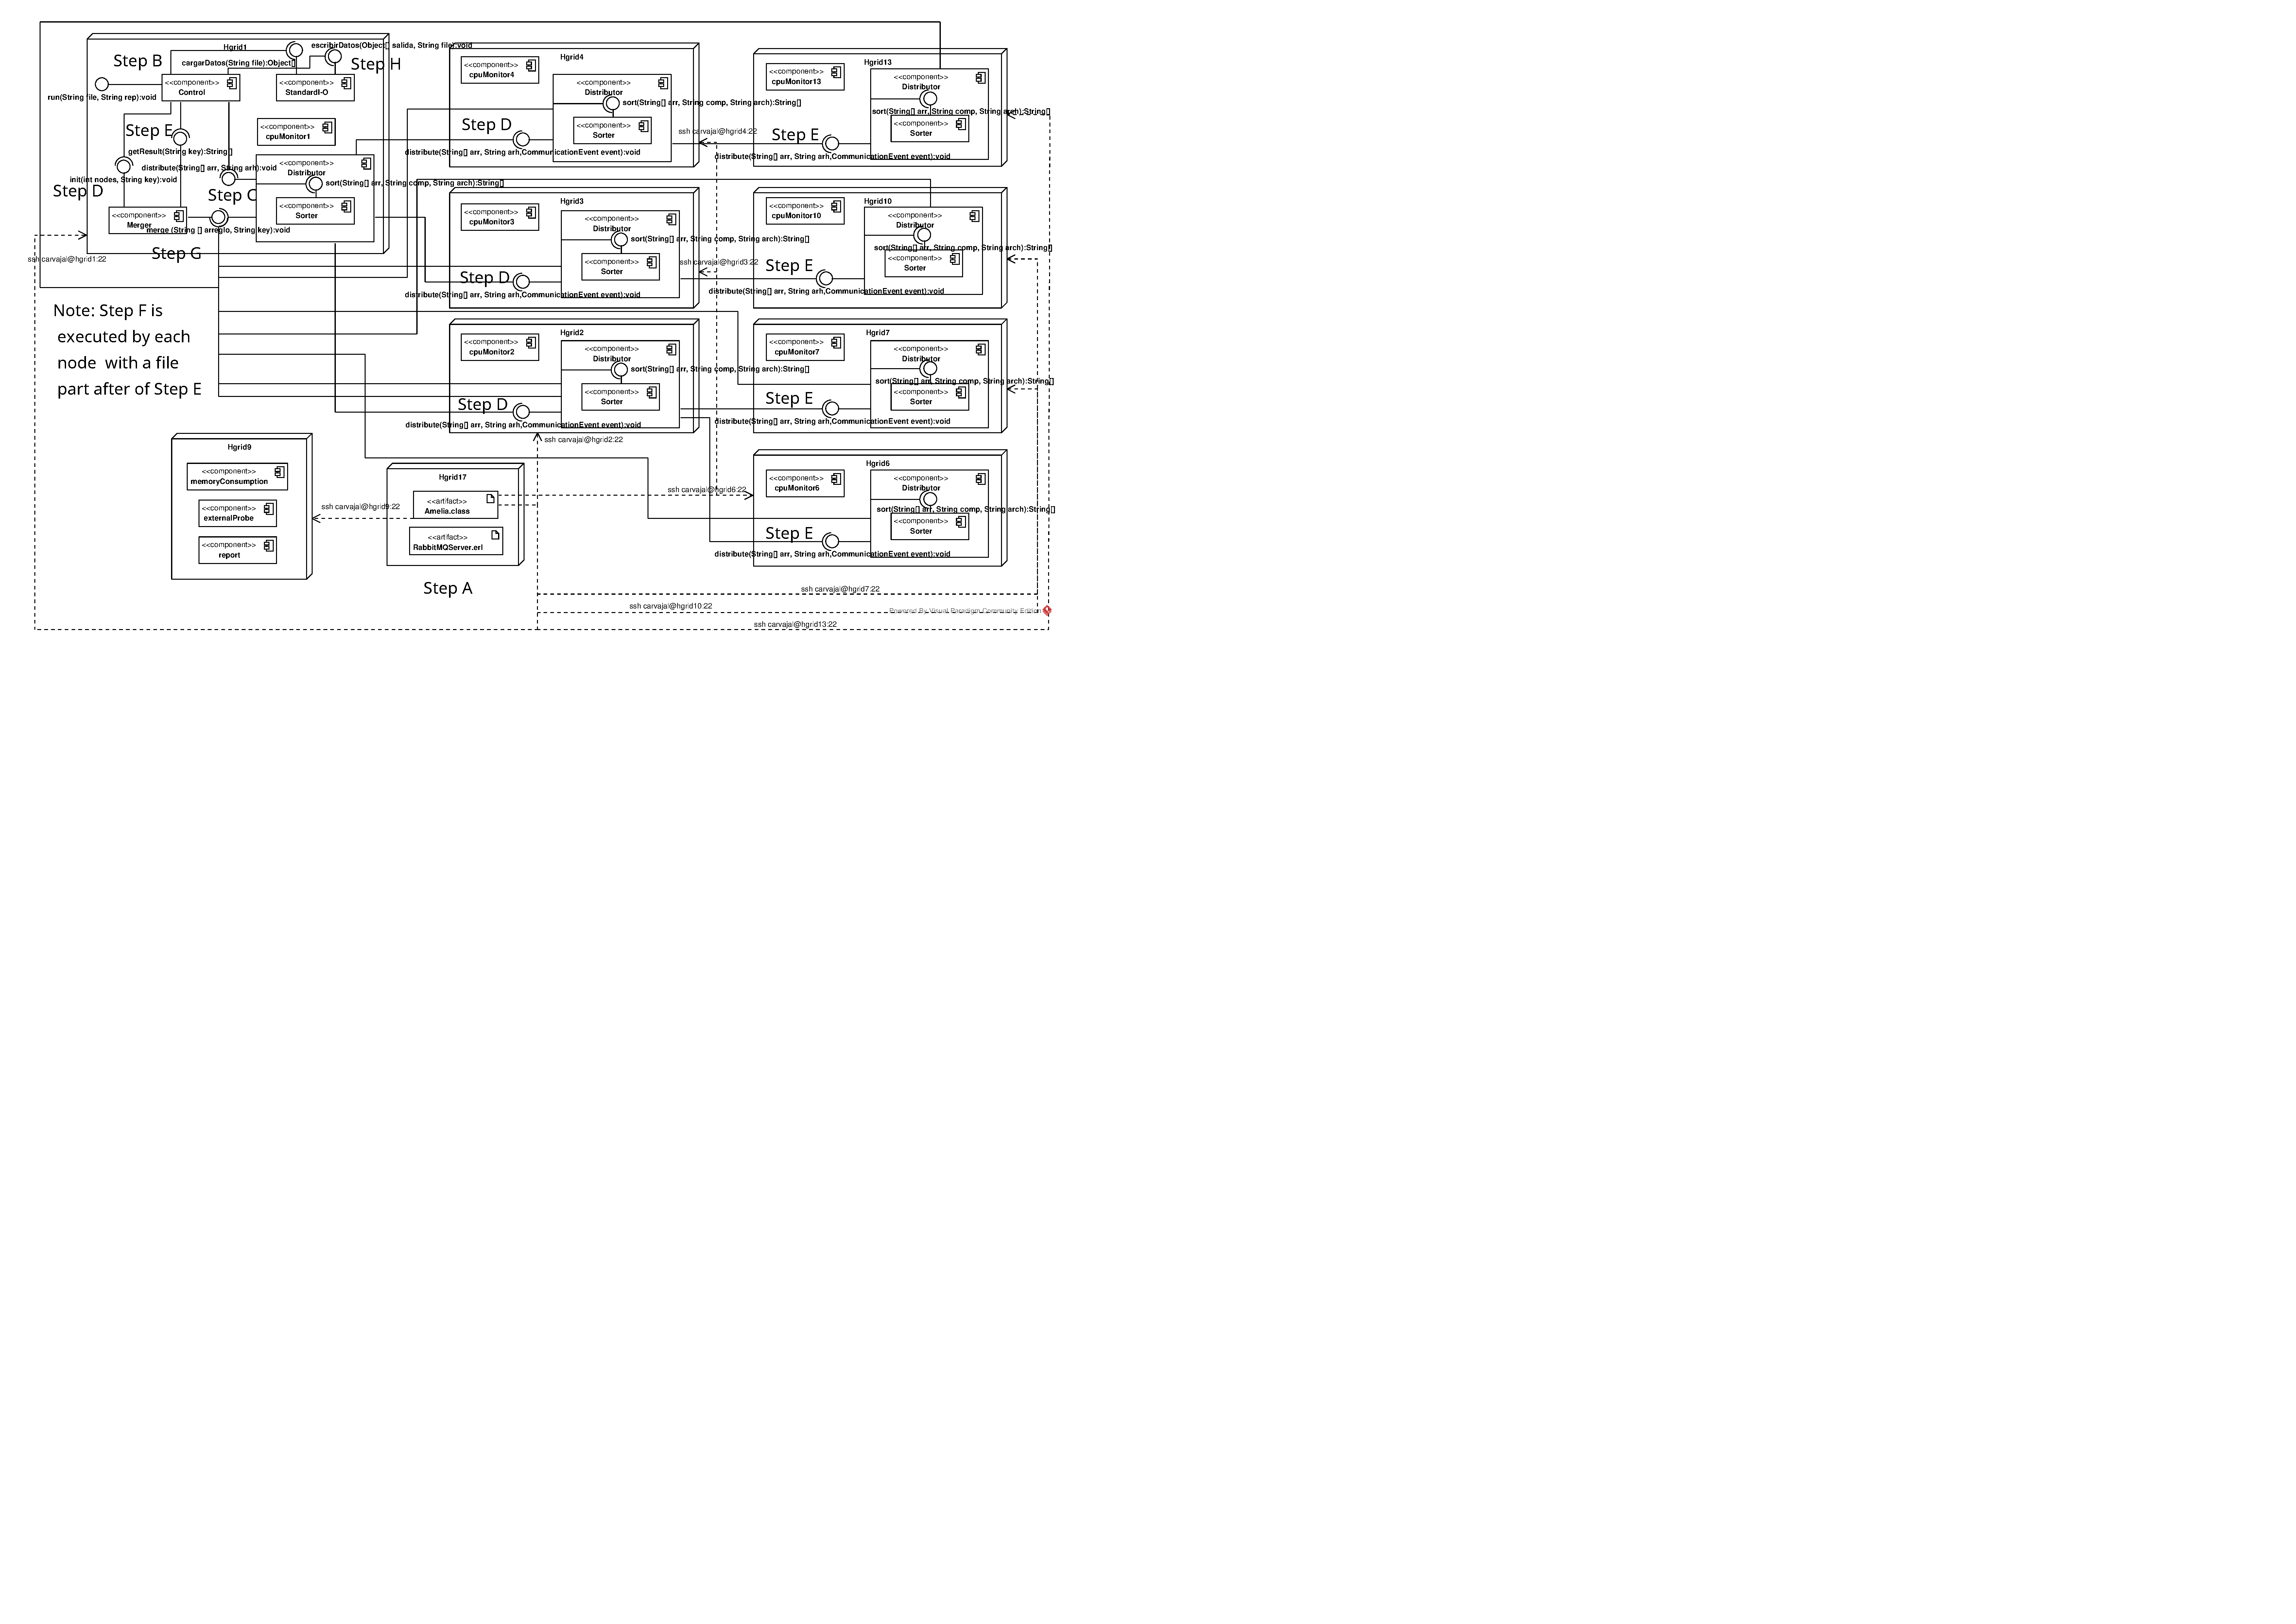
\includegraphics[trim=2cm 50cm -6cm 0cm, scale=0.46]{fig/JCMunozDistributedFJ.pdf}
		\caption{Amelia - Deployment Diagram - Fork-Join Design Pattern}
		\label{fig:diagramJCMunozDistributedFJ}
	\end{figure}
\end{landscape}

\subsubsection{Leader-Followers Design Pattern}
To implement this pattern in a distributed deployment for the sorting problem we assume three conditions. First, the asynchronous part of the pattern is realized by using threads to send requests, to simulate requests we split input data in chunks and each chunk is interpreted as a new request. Second, to avoid requests loss we implemented a request queue, which is responsible for storing requests when all processing nodes are busy. Third, to fulfill the threadpool functions we implement the LFManager component, which is responsible for managing the available processing nodes, assign them work, and manage their state changes (i.e., leader, follower, and processor). 

Figure \ref{fig:diagramJCMunozLeader-Followers} shows the deployment diagram specifying the application of this pattern.

The behavior of the Leader-Followers Design Pattern is described next:

\begin{description}
	\item [Step A] The Jmeter component of the processing node Hgrid17 starts processing when it calls the run method of the control component (processing node Hgrid1).
	\item [Step B] The control component sends to the StandardI-O component a read request to load the input file.
	\item [Step C] In this step two requests are sent. (i) the control component initializes the LFManager component; and (ii) the control component initializes the merger component.
	\item [Step D] In this step two requests are sent. (i) A new user request is registered in the queue component; and (ii) the control component sends to the merger component a request to get the whole sorted file when all file parts will be merged.
	\item [Step E] Sort requests (depending of the chunk size defined) of the user request are registered in the queue component.
	\item [Step F] The control component sends a request to the LFManager component to start the processing.
	\item [Step G] The LFManager component requests to the queue component for a sort request.
	\item [Step H] The LFManager component sends to the sorter leader component the sort request obtained from the queue component and selects a new sorter leader component. When the sort component finishes to process the sort request, it sends a request to the merge component which will merge all file parts.
	\item [Step I] The LFManager component requests to the queue component asking if there are sort requests for processing. If there are sort requests Step G, H and I are repeated until there are not sort requests to process.
	\item [Step J] The merger component receives all sorted file parts, it merges the whole sorted file and answers to the control component the request realized in Step D.
	\item [Step K] The control component receives the whole sorted file and it sends a write request to the StandardI-O component.
\end{description}

\begin{figure}[p!]
	\centering
	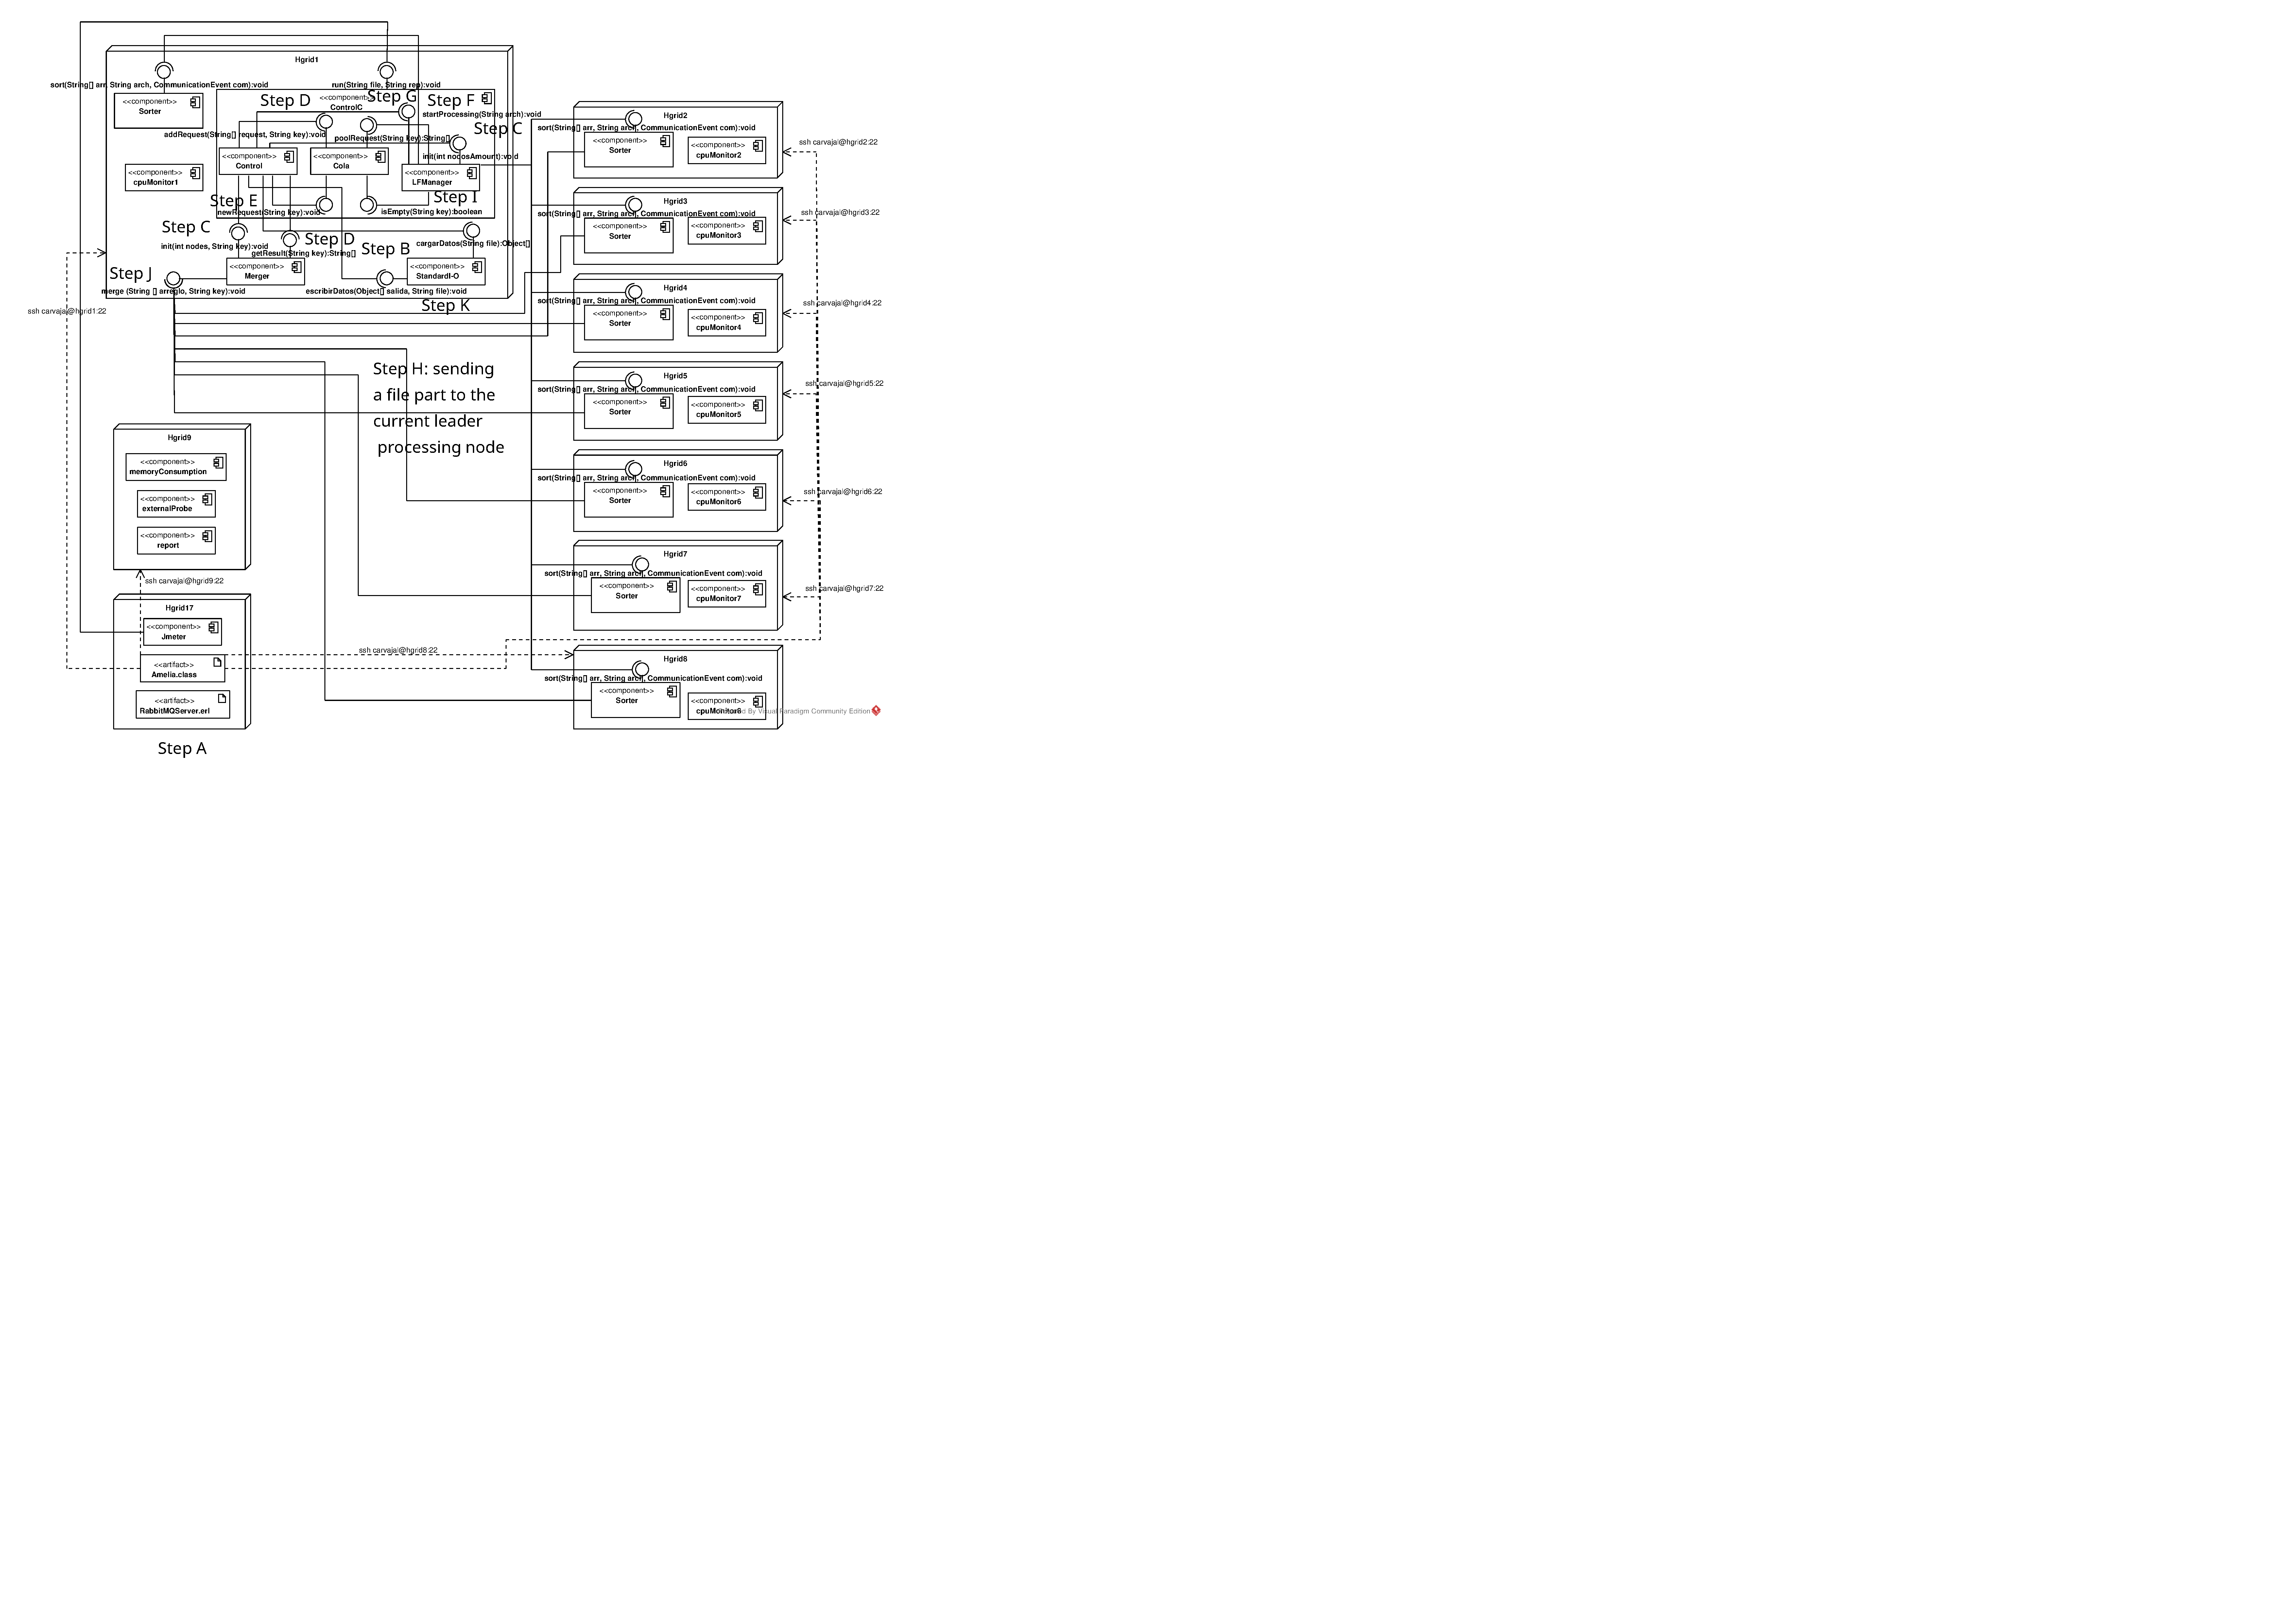
\includegraphics[trim=5cm 45cm -5cm 4cm, scale=0.45]{fig/JCMunozLeader-Followers.pdf}
	\caption{Amelia - Deployment Diagram - Leader-Followers Design Pattern}
	\label{fig:diagramJCMunozLeader-Followers}
\end{figure}

\section{Preparatory Experiments}
\label{sec:prepExperiments}
Prior to starting the execution of the designed experiments, there are two critical aspects to be defined: (i) how to distribute components along processing nodes? and (ii) which is the minimum problem size from which distribution is worth performing? These questions were proposed in previous chapter, and these must be answered before to start the experiment execution. Given that answer to these questions could vary according to each design pattern, we performed calibration experiments with each pattern.

The first question is focused mainly on locating the merge component and the components that are subsidiary to those closely related to the core solution components (i.e., Control and Standard I-O components). Components that complement experiments (i.e., probe and report components, deployment classes and the queued Server) are located in an additional node to minimize their performance effects in experiments.

The second question identifies a problem size that allows experiment results to be comparable among all design patterns and context variable scenarios, ensuring that a distributed deployment presents a better performance than in a single-machine deployment.

\subsection{Distribution of the Merge Component and the non-core System Components}
Sorting is usually solved through two phases: sort and merge. Our solution implements them in two main components, and given that we are working in a distributed deployment environment we use a third component responsible for distributing load work. Additional to our three main solution components we need two components more to sort one file: first, a component responsible for reading and writing the file, and second, a control manager component responsible for controlling interactions among all other components and receive user requests. 

Before executing the experiments, the location of each component in processing nodes must be defined (i.e., the software architecture of the system must be designed). Core components are: the Sort component responsible to sort the input file or a file part according to the Distributor component; the Distributor component, responsible to split the input file among processing nodes according to the available processing nodes; and the Merge component responsible to merge all the file parts to generate the result. Location of Sort and Distributor components is defined according to two variables: strategy or design pattern and the available processing nodes. As we mentioned before, we selected the next strategies and design patterns for our experiments: (i) the JC Sorting Strategy, (ii) the JC Sorting Strategy Variant, (iii) the Fork / Join design pattern and (iv) the Leader / Followers design pattern. Figures \ref{fig:diagramJCMunozOriStr}, \ref{fig:diagramJCMunozMergerSeparated}, \ref{fig:diagramJCMunozDistributedFJ}, and \ref{fig:diagramJCMunozLeader-Followers} determines components location of each pattern for a configuration with 8 available nodes.

The merge component is an special case because the original JC Sorting Strategy proposed one merge component for each sort component. Therefore, many merge phases were executed. However, given that merge has a complexity of O(n), having only one merge phase can improve performance. However, if there is only one merge component, where should it be located? we identify the next two possibilities (i) in the same processing node than the main distributor or (ii) in an additional processing node. For the non-core components, there are also many possible locations, and we identify the next ones (i) all non-core components in the same processing node than the main distributor (ii) each non-core component in an additional processing node, (iii) all non-core components in one additional processing node. However, option (ii) can introduce more latency and causing performance loss, thus this option was discarded.

For the remaining possible locations identified for the merge component and the non-core components, we executed calibration experiments where these components could be located in two ways, (i) all components in the same processing node than main distributor (ii) all components in an additional processing node. Table \ref{tab:optionsDescription} show these options and table \ref{tab:componentsLocation} show consolidated results of calibration experiments. Configurations 1, 2, 3 and 4 in table \ref{tab:componentsLocation} represent alternative options  of table \ref{tab:optionsDescription}. To analyze if the merge component and the non-core components should be located in an additional processing node or in the same processing node where the main distributor is located, we compared processing times using a monolithic (i.e., using only one sort component) and a distributed environments (i.e., using two sort components). For this analysis, we compared options 1 with 3 and 2 with 4 given that we first compare where we should locate components for each experiment environment. Table \ref{tab:componentsLocation} shows that in previous file sizes to highlighted cells, the option "all components in one additional processing node" is better, however, file sizes after highlighted cells are better with option "all components in the same processing node than main distributor" in both experiment environments, therefore, we decided to locate all additional components in the same processing node than the main distributor.

Other results that we observed in this experiment are: 

\begin{itemize}
	\item Comparing monolithic and distributed deployments, we can observe that depending on the used configuration the minimum file size to improve performance using distribution vary.
	\item The Norma memory structure has a better behavior than the Uma memory structure in monolithic environments and for the Fork/Join and Leader/Follower design patterns. The first observation can be explained given that these configurations do not add latency caused by access to remote data (i.e., data located in the NAS repository). The second observation must be analyzed with more experiments in the next chapter.
	\item The Leader/Followers pattern does not show a significant difference among experiments configurations, therefore, we will analyze its behavior in detail with more experiments in the next chapter.
	\item The Fork/Join design pattern improves performance in distributed deployment in almost all experiment scenarios from the most little file size. However, its performance, compared with other patterns or strategies, is the worst.
	\item The JC Sorting strategy variant and the Fork/Join Java library show the best performance in comparison with other patterns.
	\item We detect a limitation in the Norma memory structure in the monolithic deployment. In configuration where all components are located in the same processing node than the main distributor and using only one sort component (i.e., option 1) of the Fork/Join Java Library strategy we observe that from the $3'200.000$ file size, the experiments have an overload RAM memory. This overload causes a performance loss. This situation can be explained due to the memory resources consumed by all components containing additional replication of input data (i.e., local data).
\end{itemize}

% Please add the following required packages to your document preamble:
% \usepackage{graphicx}
\begin{table}[]
	\centering
	\caption{Options Description of Table \ref{tab:componentsLocation}}
	\label{tab:optionsDescription}
	\resizebox{0.5\textwidth}{!}{%
		\begin{tabular}{|c|c|}
			\hline
			\textbf{Option} & \textbf{Description} \\ \hline
			1 & \begin{tabular}[c]{@{}c@{}}All components in the same processing \\node than main distributor including only \\one sort component (Monolithic processing)\end{tabular} \\ \hline
			2 & \begin{tabular}[c]{@{}c@{}}All components in the same processing \\node than main distributor and using two \\sort components (Distributed processing)\end{tabular} \\ \hline
			3 & \begin{tabular}[c]{@{}c@{}}All components in an additional processing \\node including only one sort component \\(Monolithic processing)\end{tabular} \\ \hline
			4 & \begin{tabular}[c]{@{}c@{}}All components in an additional processing \\node and using two sort components \\(Distributed processing)\end{tabular} \\ \hline
		\end{tabular}%
	}
\end{table}

\subsection{Minimum File Size to Distribute Sorters}

To preserve comparability and to avoid executing irrelevant experiments, we executed preliminary experiments that answers the next question: Which is the minimum file size from which all selected design patterns can take advantage of distribution? Table \ref{tab:mimfileSizeEx} consolidates results of these experiments.

Results show that when the JC Sorting Strategy is configured with NORMA memory structure, it never improves their performance in a distributed deployment. In table \ref{tab:mimfileSizeEx}, for any file size used in this scenario, it can be observed that when the data is processed using 1 processing node (i.e., in the monolithic configuration) is better than using 2 processing nodes (i.e., in the distributed configuration). However, if the strategy is configured with the UMA memory structure, this strategy has a better performance in a distributed deployment in contrast to a monolithic configuration from first file size. Therefore, we decided not to execute more experiments with configuration of the JC Sorting Strategy with NORMA memory structure. 

According to the consolidated data in table \ref{tab:mimfileSizeEx}, the minimum file size from which an improvement is observed when the file is processed in a distributed environment is not uniform among all experiment scenarios. That is, each configuration can improve their performance in a distributed deployment from different file size. Highlighted cells show where each configuration starts to leverage distribution. Most of the highlighted cells are in the $200.000$ file size. However, to select the minimum file size for our experiments we decided to select a more representative minimum file size among all experiment scenarios. We take as the minimum file size that one with medium value among the largest three (i.e., $1'600.000$, $1'800.000$ and $2'200.000$). Therefore, $1'800.000$ lines is selected as the minimum file size.

In this experiment, the limitation observed in the RAM memory with the Norma memory structure in monolithic deployment in the previous experiment is also observed. This can be observed in configurations where all components are located in the same processing node that the main distributor and using only one sort component (i.e., option 1) of the Fork/Join Java Library strategy from the $3'200.000$ file size. After to analyze this behavior, we think that it is caused because in this point (file size  $3'200.000$) the RAM is overload due to the memory consumption of each component (i.e., middleware RAM requirements to deploy one component) and the file replication by each component to process their file part.

\begin{landscape}
	% Please add the following required packages to your document preamble:
	% \usepackage{multirow}
	% \usepackage{graphicx}
	% \usepackage[table,xcdraw]{xcolor}
	% If you use beamer only pass "xcolor=table" option, i.e. \documentclass[xcolor=table]{beamer}
	\begin{table}[]
		\fontsize{12}{24}\selectfont
		\centering
		\caption{Experiments for Locating Components (Latency in ms) }
		\label{tab:componentsLocation}
		\resizebox{1.45\textwidth}{!}{%
			\begin{tabular}{|c|c|c|c|c|c|c|c|c|c|c|c|c|c|c|c|c|c|c|c|c|c|c|c|c|c|c|c|c|c|c|c|c|}
				\hline
				& \multicolumn{8}{c|}{The JC Sorting Strategy Variation (ms)} & \multicolumn{8}{c|}{Fork/JoinJava library (ms)} & \multicolumn{8}{c|}{Fork-Join Design Pattern (ms)} & \multicolumn{8}{c|}{Leader-Followers Design Pattern (ms)} \\ \cline{2-33} 
				& \multicolumn{4}{c|}{Norma} & \multicolumn{4}{c|}{Uma} & \multicolumn{4}{c|}{Norma} & \multicolumn{4}{c|}{Uma} & \multicolumn{4}{c|}{Norma} & \multicolumn{4}{c|}{Uma} & \multicolumn{4}{c|}{Norma} & \multicolumn{4}{c|}{Uma} \\ \cline{2-33} 
				\multirow{-3}{*}{File Size} & 1 & 2 & 3 & 4 & 1 & 2 & 3 & 4 & 1 & 2 & 3 & 4 & 1 & 2 & 3 & 4 & 1 & 2 & 3 & 4 & 1 & 2 & 3 & 4 & 1 & 2 & 3 & 4 & 1 & 2 & 3 & 4 \\ \hline
				200.000 & 464 & 1426 & 488 & 1439 & 1423 & 804 & 1433 & 1197 & 926 & 1865 & 946 & 1868 & 1986 & 1636 & 1921 & 1303 & 937 & 965 & 1002 & 968 & \cellcolor{yellow}1968 & 1959 & \cellcolor{yellow}1994 & 1931 & 561 & 551 & 520 & 547 & \cellcolor{yellow}1425 & \cellcolor{yellow}1529 & \cellcolor{yellow}1495 & \cellcolor{yellow}1514 \\ \hline
				400.000 & 923 & 1799 & 937 & 1804 & 2831 & \cellcolor{yellow}1539 & 2791 & \cellcolor{yellow}1936 & 1378 & 2206 & 1386 & 2156 & 3452 & \cellcolor{yellow}2324 & 3226 & \cellcolor{yellow}2692 & 1917 & 2291 & 1936 & 1894 & 3848 & \cellcolor{yellow}3877 & 3959 & \cellcolor{yellow}3918 & \cellcolor{yellow}1085 & \cellcolor{yellow}1067 & \cellcolor{yellow}1113 & \cellcolor{yellow}1125 & 2777 & 3042 & 2790 & 3157 \\ \hline
				600.000 & 1475 & 2203 & 1489 & 2189 & 4241 & 2655 & 4202 & 2406 & 1810 & 2470 & 1799 & 2494 & 4930 & 2604 & 4532 & 2661 & 3473 & \cellcolor{yellow}3158 & 3444 & \cellcolor{yellow}3475 & 6326 & 3411 & 6495 & 4326 & 1668 & 1613 & 1633 & 1698 & 4177 & 4540 & 5117 & 4664 \\ \hline
				800.000 & 1953 & 2618 & 1925 & 2551 & 5715 & 3076 & 5641 & 3430 & 2176 & 2726 & 2165 & 2758 & 6241 & 3264 & 5840 & 3659 & 3816 & 3513 & 3869 & 3894 & 7705 & 4076 & 7842 & 4162 & 2202 & 2210 & 2220 & 2283 & 5554 & 6079 & 5709 & 6130 \\ \hline
				1'000.000 & 2418 & 2955 & 2356 & 2945 & 7078 & 3894 & 7012 & 3835 & 2548 & 3257 & 2511 & 3234 & 7673 & 4079 & 7081 & 4468 & 6392 & 4874 & 6376 & 6430 & 11158 & 6308 & 11650 & 6684 & 2827 & 2743 & 2755 & 2832 & 6999 & 7700 & 7347 & 7663 \\ \hline
				1'200.000 & 3095 & 3568 & 3126 & 3526 & 8768 & 5011 & 8595 & 5370 & 3196 & 3733 & 3183 & 3764 & 9181 & 4921 & 8517 & 5291 & \cellcolor{yellow}7067 & 5463 & \cellcolor{yellow}7129 & 7062 & 12823 & 7415 & 13168 & 6867 & 3478 & 3417 & 3435 & 3534 & 8464 & 9236 & 9144 & 9263 \\ \hline
				1'400.000 & 3692 & 3911 & 3623 & 3916 & 10078 & 5443 & 10031 & 5920 & 3578 & 4040 & 3548 & 3939 & 10656 & 5580 & 9899 & 5668 & 7452 & 5868 & 7530 & 7525 & 14144 & 8268 & 14661 & 7935 & 4024 & 3975 & 4010 & 4136 & 10138 & 10788 & 10692 & 10869 \\ \hline
				1'600.000 & 4233 & 4403 & 4082 & 4362 & 11627 & 6263 & 11402 & 6201 & 4050 & 4478 & 3936 & 4274 & 12105 & 6376 & 11274 & 6330 & 8031 & 6235 & 7965 & 8013 & 15580 & 9008 & 16109 & 8704 & 4654 & 4605 & 4778 & 4985 & 11277 & 12405 & 12647 & 12474 \\ \hline
				1'800.000 & 4844 & 4817 & 4669 & 4747 & \cellcolor{yellow}13062 & 6964 & \cellcolor{yellow}13102 & 7252 & 4544 & 4808 & 4468 & 4732 & 13498 & 7056 & 12931 & 7634 & 12682 & 8911 & 12754 & 12662 & 21470 & 12420 & 22055 & 11512 & 5310 & 5393 & 5328 & 5538 & 12845 & 13955 & 13380 & 13993 \\ \hline
				2'000.000 & \cellcolor{yellow}5385 & \cellcolor{yellow}5283 & \cellcolor{yellow}5548 & \cellcolor{yellow}5327 & 14611 & 7962 & 14931 & 7980 & \cellcolor{yellow}4975 & \cellcolor{yellow}5195 & \cellcolor{yellow}5317 & \cellcolor{yellow}5270 & 14992 & 8046 & 14039 & 8445 & 13318 & 9219 & 13198 & 13168 & 22608 & 12456 & 23537 & 12895 & 6049 & 6009 & 6012 & 6335 & 14394 & 15684 & 15774 & 15786 \\ \hline
				2'200.000 & 6479 & 6169 & 6824 & 6372 & 16200 & 8923 & 16780 & 9373 & 5873 & 5832 & 6333 & 5838 & 16873 & 8481 & 15843 & 9425 & 14258 & 10131 & 14430 & 14470 & 24405 & 13759 & 25210 & 13658 & 6809 & 6838 & 7143 & 7370 & 15965 & 17556 & 18047 & 17856 \\ \hline
				2'400.000 & 6864 & 6634 & 7203 & 6784 & 17656 & 9617 & 18123 & 9707 & 6443 & 6153 & 6739 & 6125 & 18247 & 9276 & 17197 & 10084 & 14684 & 10477 & 15012 & 14899 & 25910 & 14240 & 26934 & 14504 & 7499 & 7592 & 7729 & 7998 & 17561 & 19040 & 19072 & 19290 \\ \hline
				2'600.000 & 7669 & 7074 & 7884 & 7451 & 18909 & 10347 & 19462 & 10803 & 6998 & 6598 & 7651 & 6602 & 19658 & 10334 & 18724 & 10742 & 15517 & 11086 & 15625 & 15623 & 27126 & 15290 & 28095 & 16093 & 8446 & 8444 & 8827 & 8880 & 19252 & 20642 & 20460 & 21010 \\ \hline
				2'800.000 & 8244 & 7659 & 8515 & 7979 & 20591 & 11185 & 20844 & 11136 & 7640 & 7194 & 7780 & 7348 & 20906 & 10813 & 19898 & 11434 & 15962 & 11532 & 16024 & 16055 & 28516 & 16430 & 29729 & 16023 & 9165 & 9072 & 9239 & 9676 & 20328 & 22391 & 22121 & 22750 \\ \hline
				3'000.000 & 8871 & 8072 & 9264 & 9010 & 21977 & 11856 & 22723 & 12613 & 8064 & 7458 & 8659 & 7777 & 22431 & 11699 & 21966 & 12114 & 16759 & 12308 & 16789 & 17034 & 30219 & 16327 & 31070 & 17311 & 9852 & 9869 & 9925 & 10455 & 21754 & 24070 & 24108 & 24520 \\ \hline
				3'200.000 & 9523 & 8694 & 9670 & 8918 & 23497 & 12615 & 23924 & 13076 & \cellcolor{lightgray}31630 & 7885 & 8809 & 8231 & 23897 & 12033 & 22919 & 12743 & 17140 & 12577 & 17164 & 17440 & 31611 & 17268 & 32486 & 17521 & 10656 & 10557 & 10993 & 11186 & 23501 & 25602 & 25180 & 25886 \\ \hline
				3'400.000 & 10113 & 9097 & 10639 & 9122 & 24986 & 13445 & 25406 & 14222 & \cellcolor{lightgray}61993 & 8054 & 9866 & 8125 & 25286 & 12451 & 24588 & 14336 & 26349 & 17695 & 26747 & 26619 & 42282 & 23535 & 43747 & 23866 & 11423 & 11325 & 11365 & 12005 & 24878 & 27470 & 26567 & 27867 \\ \hline
				3'600.000 & 10495 & 9543 & 10920 & 9765 & 26362 & 14464 & 27436 & 15062 & \cellcolor{lightgray}18039 & 9142 & 9978 & 9559 & 26873 & 14827 & 25791 & 15513 & 26975 & 18112 & 27103 & 26973 & 43677 & 23684 & 45173 & 24952 & 12012 & 12077 & 12032 & 12423 & 26430 & 28969 & 28841 & 29456 \\ \hline
				3'800.000 & 11015 & 9994 & 11566 & 10499 & 27957 & 15292 & 28872 & 16381 & \cellcolor{lightgray}17897 & 10093 & 11233 & 10130 & 28383 & 14607 & 27181 & 15937 & 29124 & 18596 & 27852 & 27930 & 45059 & 25153 & 46789 & 25351 & 12901 & 12808 & 12801 & 13404 & 28344 & 30988 & 30932 & 31379 \\ \hline
				4'000.000 & 11873 & 10582 & 11788 & 10875 & 29674 & 16549 & 30502 & 16887 & \cellcolor{lightgray}76094 & 11536 & 11119 & 9864 & 29623 & 15589 & 28483 & 16421 & 43984 & 19495 & 28213 & 28622 & 46591 & 25988 & 48440 & 25896 & 13424 & 13540 & 13931 & 13985 & 29443 & 32340 & 33703 & 33259 \\ \hline
			\end{tabular}%
		}
	\end{table}
\end{landscape}

\begin{landscape}
	% Please add the following required packages to your document preamble:
	% \usepackage{multirow}
	% \usepackage{graphicx}
	\begin{table}[]
		\fontsize{10}{18}\selectfont
		\textmd
		\centering
		\caption{Minimum File Size Experiment}
		\label{tab:mimfileSizeEx}
		\resizebox{1.4\textwidth}{!}{%
			\begin{tabular}{|c|c|c|c|c|c|c|c|c|c|c|c|c|c|c|c|c|c|c|c|c|}
				\hline
				\multirow{3}{*}{\begin{tabular}[c]{@{}c@{}}File\\   Size\end{tabular}} & \multicolumn{4}{c|}{The JC Sorting Strategy} & \multicolumn{4}{c|}{The JC Sorting Variation} & \multicolumn{4}{c|}{Fork/Join Java library} & \multicolumn{4}{c|}{Fork-Join Design Pattern} & \multicolumn{4}{c|}{Leader-Followers Design Pattern } \\ \cline{2-21} 
				& \multicolumn{2}{c|}{NORMA} & \multicolumn{2}{c|}{UMA} & \multicolumn{2}{c|}{NORMA} & \multicolumn{2}{c|}{UMA} & \multicolumn{2}{c|}{NORMA} & \multicolumn{2}{c|}{UMA} & \multicolumn{2}{c|}{NORMA} & \multicolumn{2}{c|}{UMA} & \multicolumn{2}{c|}{NORMA} & \multicolumn{2}{c|}{UMA} \\ \cline{2-21} 
				& 1 & 2 & 1 & 2 & 1 & 2 & 1 & 2 & 1 & 2 & 1 & 2 & 1 & 2 & 1 & 2 & 1 & 2 & 1 & 2 \\ \hline
				200.000 & 436 & 469 & \cellcolor{yellow}1360 & \cellcolor{yellow}832 & 464 & 1426 & \cellcolor{yellow}1423 & \cellcolor{yellow}804 & 926 & 1865 & \cellcolor{yellow}1986 & \cellcolor{yellow}1636 & 937 & 965 & 1968 & 1959 & \cellcolor{yellow}561 & \cellcolor{yellow}551 & 1425 & 1529 \\ \hline
				400.000 & 776 & 864 & 2613 & 1587 & 923 & 1799 & 2831 & 1539 & 1378 & 2206 & 3452 & 2324 & 1917 & 2291 & 3848 & 3877 & 1085 & 1067 & 2777 & 3042 \\ \hline
				600.000 & 1299 & 1364 & 3905 & 2381 & 1475 & 2203 & 4241 & 2655 & 1810 & 2470 & 4930 & 2604 & \cellcolor{yellow}3473 & \cellcolor{yellow}3158 & \cellcolor{yellow}6326 & \cellcolor{yellow}3411 & 1668 & 1613 & 4177 & 4540 \\ \hline
				800.000 & 1630 & 1829 & 5224 & 3149 & 1953 & 2618 & 5715 & 3076 & 2176 & 2726 & 6241 & 3264 & 3816 & 3513 & 7705 & 4076 & 2202 & 2210 & 5554 & 6079 \\ \hline
				1.000.000 & 2108 & 2276 & 6489 & 3935 & 2418 & 2955 & 7078 & 3894 & 2548 & 3257 & 7673 & 4079 & 6392 & 4874 & 11158 & 6308 & 2827 & 2743 & 7074 & 7030 \\ \hline
				1.200.000 & 2779 & 2954 & 7857 & 4797 & 3095 & 3568 & 8768 & 5011 & 3196 & 3733 & 9181 & 4921 & 7067 & 5463 & 12823 & 7415 & 3478 & 3417 & 8623 & 8619 \\ \hline
				1.400.000 & 3134 & 3550 & 9177 & 5623 & 3692 & 3911 & 10078 & 5443 & 3578 & 4040 & 10656 & 5580 & 7452 & 5868 & 14144 & 8268 & 4024 & 3975 & 9993 & 10050 \\ \hline
				1.600.000 & 3703 & 3965 & 10532 & 6375 & 4233 & 4403 & 11627 & 6263 & 4050 & 4478 & 12105 & 6376 & 8031 & 6235 & 15580 & 9008 & 4654 & 4605 & \cellcolor{yellow}11473 & \cellcolor{yellow}11447 \\ \hline
				1.800.000 & 4167 & 4895 & 11847 & 7204 & \cellcolor{yellow}4844 & \cellcolor{yellow}4817 & 13062 & 6964 & 4544 & 4808 & 13498 & 7056 & 12682 & 8911 & 21470 & 12420 & 5310 & 5393 & 12843 & 12935 \\ \hline
				2.000.000 & 4666 & 5274 & 13301 & 7973 & 5385 & 5283 & 14611 & 7962 & 4975 & 5195 & 14992 & 8046 & 13318 & 9219 & 22608 & 12456 & 6049 & 6009 & 14249 & 14612 \\ \hline
				2.200.000 & 5520 & 6255 & 14780 & 8928 & 6479 & 6169 & 16200 & 8923 & \cellcolor{yellow}5873 & \cellcolor{yellow}5832 & 16873 & 8481 & 14258 & 10131 & 24405 & 13759 & 6809 & 6838 & 15881 & 15952 \\ \hline
				2.400.000 & 11167 & 8710 & 16077 & 9751 & 6864 & 6634 & 17656 & 9617 & 6443 & 6153 & 18247 & 9276 & 14684 & 10477 & 25910 & 14240 & 7499 & 7592 & 17291 & 17530 \\ \hline
				2.600.000 & 32477 & 33541 & 17446 & 10542 & 7669 & 7074 & 18909 & 10347 & 6998 & 6598 & 19658 & 10334 & 15517 & 11086 & 27126 & 15290 & 8446 & 8444 & 18810 & 18854 \\ \hline
				2.800.000 & 29485 & 40926 & 18745 & 11340 & 8244 & 7659 & 20591 & 11185 & 7640 & 7194 & 20906 & 10813 & 15962 & 11532 & 28516 & 16430 & 9165 & 9072 & 20185 & 20323 \\ \hline
				3.000.000 & 36953 & 117483 & 20078 & 12172 & 8871 & 8072 & 21977 & 11856 & 8064 & 7458 & 22431 & 11699 & 16759 & 12308 & 30219 & 16327 & 9852 & 9869 & 21411 & 21744 \\ \hline
				3.200.000 & 38117 & 206397 & 21387 & 13010 & 9523 & 8694 & 23497 & 12615 & \cellcolor{lightgray}31630 & 7885 & 23897 & 12033 & 17140 & 12577 & 31611 & 17268 & 10656 & 10557 & 22859 & 23042 \\ \hline
				3.400.000 & 271451 & 240498 & 22851 & 13629 & 10113 & 9097 & 24986 & 13445 & \cellcolor{lightgray}61993 & 8054 & 25286 & 12451 & 26349 & 17695 & 42282 & 23535 & 11423 & 11325 & 24941 & 25139 \\ \hline
				3.600.000 & 44432 & 292747 & 24287 & 14571 & 10495 & 9543 & 26362 & 14464 & \cellcolor{lightgray}18039 & 9142 & 26873 & 14827 & 26975 & 18112 & 43677 & 23684 & 12012 & 12077 & 26220 & 26417 \\ \hline
				3.800.000 & 65956 & 423089 & 25669 & 15465 & 11015 & 9994 & 27957 & 15292 & \cellcolor{lightgray}17897 & 10093 & 28383 & 14607 & 29124 & 18596 & 45059 & 25153 & 12901 & 12808 & 27598 & 28020 \\ \hline
				4.000.000 & 191262 & 551244 & 27053 & 16363 & 11873 & 10582 & 29674 & 16549 & \cellcolor{lightgray}76094 & 11536 & 29623 & 15589 & 43984 & 19495 & 46591 & 25988 & 13424 & 13540 & 28854 & 29209 \\ \hline
			\end{tabular}%
		}
	\end{table}
\end{landscape}

%\subsection{Batch Size to Fork/Join and Leader/Followers Design Patterns}%

\section{Control Tests}
\label{sec:controlTest}

To ensure that our experiments are not affected by unknown or irrelevant variables, we executed the same test repeatedly during a whole day. This is a control and calibration test. In this test, we expected no atypical results that suggest that there are environment variables which can affect our experiments.

Test was executed 4000 times. Execution time varied between 8038 and 9532 milliseconds, that is a range of 1494 milliseconds. This variation suggests that there are not other variables that affect our experiments. Figure \ref{fig:pruebaControl} also shows this test results.

Additionally, the configuration described in section \ref{sec:confandControl} was tested, and we observe that results were the expected, that is, this test was executed in the expected time range. If results were not between the expected results, we would have calibrated the configuration until achieving the expected results.

\begin{landscape}
	\begin{figure}[p!]
		\centering
		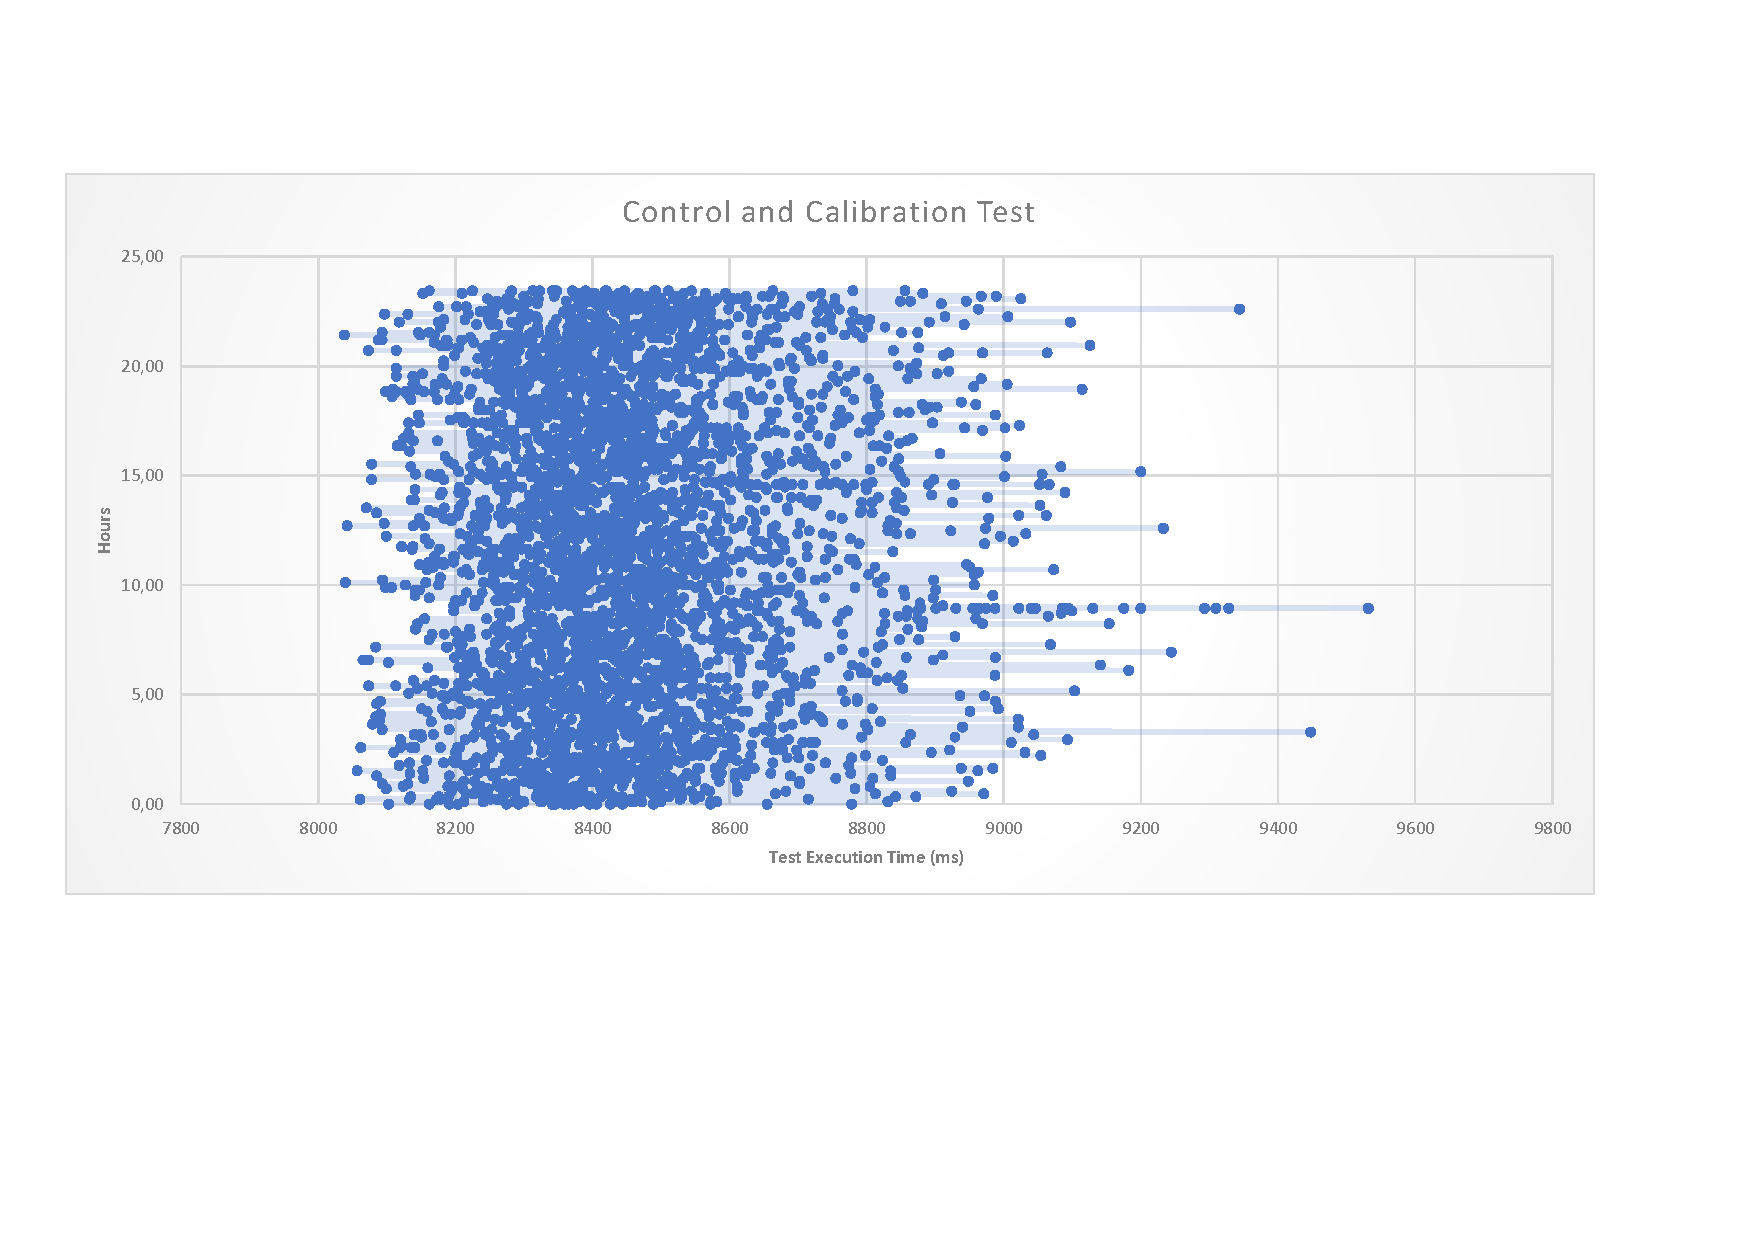
\includegraphics[trim=1cm 5cm 5cm 1cm, scale=0.9]{fig/PruebaControl.pdf}
		\caption{Control Tests Graph}
		\label{fig:pruebaControl}
	\end{figure}
\end{landscape}

\section{Experiments Execution}
Using the Amelia class files we automated the tests execution: in total, this amounts to 2535 experiments for the latency analysis and 324 for the throughput. The Liason laboratory was used during 24 hours for approximately two months with short pauses each two days.

For the throughput analysis, we decided to use only the four best configurations selected among the latency analysis. Additionally, only 11 different file sizes used, from $1'800.000$ lines until $9'800.000$ lines adding $800.000$ lines to each file. The experiments were repeated two times and results averaged, due to in the throughput experiments could exist little variations because many requests are sent at the same time and we did not control to send and neither arrive sequence.

The experiments results will be analyzed in the next chapter.

\section{Chapter Summary}
In this chapter, we executed the experiments designed in the before chapter. To execute these experiments we required to follow the next phases: first, we configured and controlled items like hardware, operating system, precision time protocol (it coordinates the time among the processing units to ensure the reliability in the taken measurements), among others. Second, we defined the software deployment configuration. Third, we executed preparatory experiments to define invariant values to execute all experiments like the minimum problem size and the additional component distribution. Fourth, we executed a control test to validate that there are not variables that can affect the experiment's measurements and results. And finally, we executed the experiments.










	% =========================================================================
	\chapter{Analysis of Computational Experiments}
	\label{cha:experimentAnalysis}
	Following design of experiments described in chapter \ref{cha:experimentDesign}, we execute more than 2000 experiments, in this chapter we summarize and analyze results of experiments. Analysis is divided in three sections, (i) behavior of case of study, (ii) experiments focused in latency, and (iii) experiments focused in throughput. 

\section{The Sorting Solution Phases Characterized}
We configured all the solutions involving the different design patterns with the same phases. However, the processing time of each phase can vary according to the design pattern used. To characterize the sorting solution phases, we compute the percentage of each phase with respect to the total time to process one file. We consolidate the data in table \ref{tab:designPatternsBehavior} including minimum, maximum, range, and the average of the processing times' percentage of each phase. 

%(the sort time and the read time percentage are computed, but these are contained in the distribution phase time)

We identify the next phases; (i) sort, (ii) read, (iii) communication among the distribution components, (iv) merge, (v) write, and (vi) distribution. The sort phase is responsible to apply the QuickSort algorithm implemented by the Java Array Class to the data. The read phase is responsible to load the file to memory in the Norma memory structure configurations and to identify the file size in the UMA memory structure configurations (each processing node is responsible to read its own data part). The communication phase among the distribution components (from now this phase also to be known as the communication phase) is responsible to measure how much time is used to communicate the processing units. The merge component is responsible to merge all data parts that were distributed when configuration defines to use more than one processing node. The write phase is responsible to write the data sorted, that is the application output. Finally, the distribution phase is responsible to decide if data should be divide or send to be sorted (the sort phase always is contained in the distribution phase. When the test is configured with the UMA memory structure, the read phase also is contained in the distribution phase). Despite we used QickSort into the processing units, our implementations are similar to the mergeSort algorithm due to the distribution, sort and merge phases.

% Please add the following required packages to your document preamble:
% \usepackage{multirow}
% \usepackage{graphicx}
\begin{table}[]
	\fontsize{12}{20}\selectfont
	\centering
	\caption{Sorting Phases: Distribution Time per Design Pattern}
	\label{tab:designPatternsBehavior}
	\resizebox{\textwidth}{!}{%
		\begin{tabular}{|c|c|c|c|c|c|c|c|c|c|c|c|}
			\hline
			\multicolumn{3}{|c|}{\begin{tabular}[c]{@{}c@{}}DESIGN PATTERN \\ EXPERIMENT CONFIGURATION\end{tabular}} & SORT & READ & COMM & MERGE & WRITE & DISTRIBUTION &
			{\begin{tabular}[c]{@{}c@{}c@{}}COMM \\CONTROL \\WRITE\end{tabular}}  & {\begin{tabular}[c]{@{}c@{}}WAIT\\ MERGE\end{tabular}} & {\begin{tabular}[c]{@{}c@{}c@{}}COMM \\MERGE\\CONTROL\end{tabular}} \\ \hline
			\multirow{12}{*}{\begin{tabular}[c]{@{}c@{}}THE JC SORTING \\ STRATEGY  (UMA)\end{tabular}} & \multirow{4}{*}{ICE} 
			& MIN & 7\% & 6\% & 0\% & 0\% & 9\% & 27\% & 3\% & 0\% & 15\% \\ \cline{3-12} 
			&  & MAX & 31\% & 10\% & 31\% & 8\% & 21\% & 70\% & 7\% & 0\% & 23\% \\ \cline{3-12} 
		%	&  & RANGE & 23,55\% & 3\% & 31\% & 8\% & 11\% & 43\% & 4\% & 0,00\% & 7\% \\ \cline{3-12} 
			&  & AVERAGE & 15\% & 7\% & 19\% & 4\% & 14\% & 41\% & 4\% & 0\% & 15\% \\ \cline{2-12} 
			& \multirow{4}{*}{RMI} & MIN & \cellcolor{yellow}5\% & 4\% & 0\% & 0\% & 5\% & 22\% & 11\% & 0\% & 22\% \\ \cline{3-12} 
			&  & MAX & 24\% & 9\% & 29\% & 2\% & 15\% & 51\% & 32\% & 0\% & 32\% \\ \cline{3-12} 
		%	&  & RANGE & 19\% & 4\% & 29\% & 2\% & 10\% & 29\% & 21\% & 0\% & 10\% \\ \cline{3-12} 
			&  & AVERAGE & \cellcolor{yellow}11\% & 6\% & 16\% & 0\% & 8\% & 31\% & 18\% & 0\% & 23\% \\ \cline{2-12} 
			& \multirow{4}{*}{REST} & MIN & 9\% & 7\% & 30\% & 0\% & 10\% & 11\% & 0\% & 0\% & 19\% \\ \cline{3-12} 
			&  & MAX & 25\% & 10\% & 43\% & 6\% & 15\% & 53\% & 0\% & 11\% & 33\% \\ \cline{3-12} 
		%	&  & RANGE & 15\% & 2\% & 13\% & 6\% & 5\% & 42\% & 0\% & 11\% & 14\% \\ \cline{3-12} 
			&  & AVERAGE & 15\% & 9\% & 37\% & 3\% & 12\% & 25\% & 0\% & 3\% & 18\% \\ \hline
			\multirow{12}{*}{\begin{tabular}[c]{@{}c@{}}THE JC SORTING \\ STRATEGY  \\ VARIATION - \\ SEPARATION OF \\ THE MERGE \\ COMPONENT\end{tabular}} & \multirow{4}{*}{ICE} & MIN & 11\% & 2\% & 0\% & 0\% & 3\% & 20\% & 4\% & 0\% & 13\% \\ \cline{3-12} 
			&  & MAX & 28\% & 11\% & 44\% & 17\% & 21\% & 61\% & 7\% & 8\% & 25\% \\ \cline{3-12} 
		%	&  & RANGE & 16\% & 8\% & 44\% & 16\% & 17\% & 40\% & 3\% & 8\% & 12\% \\ \cline{3-12} 
			&  & AVERAGE & 19\% & 7\% & 11\% & 6\% & 12\% & 37\% & 6\% & 5\% & 20\% \\ \cline{2-12} 
			& \multirow{4}{*}{RMI} & MIN & 9\% & 3\% & 0\% & 0\% & 2\% & 15\% & 11\% & 0\% & 16\% \\ \cline{3-12} 
			&  & MAX & 17\% & 9\% & 72\% & 10\% & 12\% & 53\% & 25\% & 5\% & 32\% \\ \cline{3-12} 
		%	&  & RANGE & 7\% & 5\% & 72\% & 9\% & 9\% & 38\% & 14\% & 5\% & 15\% \\ \cline{3-12} 
			&  & AVERAGE & 14\% & 5\% & 16\% & 3\% & 6\% & 30\% & 17\% & 3\% & 22\% \\ \cline{2-12} 
			& \multirow{4}{*}{REST} & MIN & 13\% & 1\% & 21\% & 0\% & 1\% & 22\% & 0\% & 0\% & 0\% \\ \cline{3-12} 
			&  & MAX & 20\% & 11\% & 69\% & 8\% & 18\% & 65\% & 0\% & 9\% & 0\% \\ \cline{3-12} 
		%	&  & RANGE & 6\% & 9\% & 48\% & 8\% & 16\% & 42\% & 0\% & 9\% & 0\% \\ \cline{3-12} 
			&  & AVERAGE & 16\% & 5\% & 47\% & 2\% & 8\% & 37\% & 0\% & 3\% & 0\% \\ \hline
			\multirow{12}{*}{\begin{tabular}[c]{@{}c@{}}THE FORK / JOIN \\ JAVA LIBRARY\end{tabular}} & \multirow{4}{*}{ICE} & MIN & 16\% & 3\% & 0\% & 1\% & 3\% & 26\% & 3\% & 0\% & 11\% \\ \cline{3-12} 
			&  & MAX & 20\% & 12\% & 46\% & 9\% & 21\% & 52\% & 7\% & 13\% & 25\% \\ \cline{3-12} 
		%	&  & RANGE & 4\% & 9\% & 46\% & 7\% & 17\% & 26\% & 3\% & 13\% & 13\% \\ \cline{3-12} 
			&  & AVERAGE & 18\% & 8\% & 12\% & 3\% & 13\% & 37\% & 6\% & 5\% & 21\% \\ \cline{2-12} 
			& \multirow{4}{*}{RMI} & MIN & 9\% & 3\% & 0\% & 0\% & 2\% & 20\% & 0\% & 0\% & 0\% \\ \cline{3-12} 
			&  & MAX & 18\% & 11\% & 54\% & 9\% & 13\% & 45\% & 24\% & 8\% & 30\% \\ \cline{3-12} 
		%	&  & RANGE & 8\% & 8\% & 54\% & 8\% & 11\% & 24\% & 24\% & 7\% & 30\% \\ \cline{3-12} 
			&  & AVERAGE & 13\% & 5\% & 24\% & 2\% & 7\% & 30\% & 13\% & 4\% & 17\% \\ \cline{2-12} 
			& \multirow{4}{*}{REST} & MIN & 11\% & 2\% & 24\% & 0\% & 1\% & 24\% & 0\% & 1\% & 0\% \\ \cline{3-12} 
			&  & MAX & 18\% & 9\% & 66\% & 8\% & 16\% & 60\% & 0\% & 10\% & 0\% \\ \cline{3-12} 
		%	&  & RANGE & 7\% & 7\% & 42\% & 7\% & 15\% & 36\% & 0\% & 9\% & 0\% \\ \cline{3-12} 
			&  & AVERAGE & 16\% & 5\% & 46\% & 2\% & 8\% & 37\% & 0\% & 4\% & 0\% \\ \hline
			\multirow{12}{*}{\begin{tabular}[c]{@{}c@{}}THE FORK / JOIN \\ DESIGN PATTERN\end{tabular}} & \multirow{4}{*}{ICE} & MIN & 18\% & 1\% & 0\% & 8\% & 1\% & 25\% & 1\% & 0\% & 5\% \\ \cline{3-12} 
			&  & MAX & \cellcolor{yellow}43\% & 30\% & 33\% & 25\% & 12\% & 80\% & 4\% & 10\% & 15\% \\ \cline{3-12} 
		%	&  & RANGE & 24\% & 28\% & 33\% & 17\% & 10\% & 55\% & 2\% & 10\% & 10\% \\ \cline{3-12} 
			&  & AVERAGE & \cellcolor{yellow}28\% & 13\% & 8\% & 17\% & 5\% & 51\% & 2\% & 3\% & 10\% \\ \cline{2-12} 
			& \multirow{4}{*}{RMI} & MIN & 12\% & 2\% & 0\% & 5\% & 2\% & 16\% & 2\% & 0\% & 13\% \\ \cline{3-12} 
			&  & MAX & 32\% & 26\% & 46\% & 9\% & 8\% & 63\% & 17\% & 4\% & 21\% \\ \cline{3-12} 
		%	&  & RANGE & 20\% & 24\% & 46\% & 4\% & 6\% & 47\% & 14\% & 4\% & 8\% \\ \cline{3-12} 
			&  & AVERAGE & 20\% & 10\% & 25\% & 7\% & 4\% & 34\% & 8\% & 2\% & 17\% \\ \cline{2-12} 
			& \multirow{4}{*}{REST} & MIN & 15\% & 1\% & 6\% & 4\% & 1\% & 20\% & 0\% & 0\% & 10\% \\ \cline{3-12} 
			&  & MAX & 33\% & 28\% & 56\% & 9\% & 7\% & 68\% & 4\% & 4\% & 17\% \\ \cline{3-12} 
		%	&  & RANGE & 18\% & 26\% & 50\% & 4\% & 6\% & 48\% & 4\% & 3\% & 7\% \\ \cline{3-12} 
			&  & AVERAGE & 23\% & 12\% & 29\% & 6\% & 4\% & 41\% & 1\% & 2\% & 14\% \\ \hline
			\multirow{12}{*}{\begin{tabular}[c]{@{}c@{}}THE LEADER / FOLLOWERS \\ DESIGN PATTERN\end{tabular}} & \multirow{4}{*}{ICE} & MIN & 15\% & 1\% & 31\% & 0\% & 2\% & 36\% & 2\% & 0\% & 7\% \\ \cline{3-12} 
			&  & MAX & 28\% & 18\% & 38\% & 2\% & 9\% & 50\% & 3\% & 0\% & 12\% \\ \cline{3-12} 
		%	&  & RANGE & 13\% & 17\% & 6\% & 2\% & 7\% & 13\% & 1\% & 0\% & 4\% \\ \cline{3-12} 
			&  & AVERAGE & 23\% & 9\% & 35\% & 2\% & 5\% & 44\% & 2\% & 0\% & 9\% \\ \cline{2-12} 
			& \multirow{4}{*}{RMI} & MIN & 17\% & 1\% & 33\% & 1\% & 1\% & 33\% & 0\% & 0\% & 0\% \\ \cline{3-12} 
			&  & MAX & 24\% & 17\% & 49\% & 2\% & 5\% & 38\% & 12\% & 3\% & 13\% \\ \cline{3-12} 
	%		&  & RANGE & 6\% & 16\% & 16\% & 0\% & 4\% & 5\% & 12\% & 3\% & 13\% \\ \cline{3-12} 
			&  & AVERAGE & 21\% & 9\% & 42\% & 1\% & 3\% & 36\% & 6\% & 1\% & 7\% \\ \cline{2-12} 
			& \multirow{4}{*}{REST} & MIN & 24\% & 1\% & 21\% & 1\% & 1\% & 51\% & 0\% & 0\% & 0\% \\ \cline{3-12} 
			&  & MAX & 30\% & 24\% & 43\% & 3\% & 11\% & 66\% & 0\% & 1\% & 0\% \\ \cline{3-12} 
		%	&  & RANGE & 6\% & 23\% & 22\% & 2\% & 9\% & 14\% & 0\% & 1\% & 0\% \\ \cline{3-12} 
			&  & AVERAGE & 27\% & 13\% & 32\% & 2\% & 5\% & 59\% & 0\% & 0\% & 0\% \\ \hline
		\end{tabular}%
	}
\end{table}

However, during the data analysis, we identify three additional phases, (i) waiting for merge, (ii) communication between the merge component and the control component, and (iii) communication between the control component and the write component. The communication time between the merge component and the control component occurs when the sorted data is sent to the control component. The communication between the control component and the writer component occurs when the sorted data is sent to be written. In the Uma configuration, these times take a huge part of the total time because this phase transmits the biggest amount of data in the process. The waiting for merge time occurs when the merge component sleeps while all data parts arrive to be merged. The merge component wakes up each second to verify if the merge phase can start.

Table \ref{tab:designPatternsBehavior} summarizes the experiments results used to characterize the sorting solution phases. To consolidate the experiment results we use the average of collected data respect to (i) the number of available nodes, (ii) the file size and (iii) the memory structures. These variables have a dispersion range less than variables: (i) the communication protocol, and (ii) the design pattern or strategy. This table shows the minimum, the maximum and the average of the percentage time needed to execute each phase.

The phases with more variation range according to table \ref{tab:designPatternsBehavior} is the communication and distribution phases. However, through more detailed data (annex), where the number of available nodes and memory structure are discriminated, we observe that (i) the more amount of available nodes the more communication phase time is increased and the distribution and sort phases time are decreased; (ii) the read phase time is not included into the distribution phase time in configurations with NORMA memory structure, (iii) the wait merge time is just measured in strategies or design patterns where the merger component is just one.

When the sorting problem is solved using a monolithic configuration (i.e., using only one processing node), the main phases are the sort and the merge, and additionally, there are complementary phases such are read and write. However, if the sorting problem is solved in a distributed environment new phases are introduced, such as distribution and communication phases. According to table  \ref{tab:designPatternsBehavior} in a distributed environment these new phases could take more than $50\%$ of the needed time to solve the problem. But, this situation does not necessarily indicate that distribution affects negatively the solution performance. Despite the new phases take more time than the main phases (i.e., sort and merge phases) time needed to solve the problem in a distributed environment versus a monolithic environment is less as file size increasing.

Dispersion range in phases sort, merge, read, write, and comm merge/control is explained by the file size variable mainly. Because as bigger is the file more time is needed for each of these phases. However, the distribution and communication phases are affected by more variables, such as the communication protocol, the design pattern or strategy applied, the memory structure, the file size, and the number of available nodes. The communication protocol affects the time to communicate any two processing nodes, thus it affects the distribution phase too. The design pattern or strategy applied defines the system behavior to distribute processing, some of them could be more efficient than others (this situation will be analyzed in section \ref{subsec:designPatternsAnalysis}).  According to the memory structure variable, data travel through processing nodes (NORMA) or each processing node is responsible to read and process only its file part (UMA), this situation affects the communication time and the distribution time. The file size and the number of available nodes variables affect the distribution and communication phases because as bigger is any of them more time is needed to distribute processing.

%To illustrate the behavior of each phase, we use the figures \ref{fig:originalStrategyBehaviorIce}, \ref{fig:originalStrategyBehaviorRest}, \ref{fig:originalStrategyBehaviorRmi}, \ref{fig:variationOriginalStrategyBehaviorIce}, \ref{fig:variationOriginalStrategyBehaviorRest}, \ref{fig:variationOriginalStrategyBehaviorRmi}, \ref{fig:forkJoinLibraryBehaviorIce}, \ref{fig:forkJoinLibraryBehaviorRest}, \ref{fig:forkJoinLibraryBehaviorRmi}, \ref{fig:forkJoinBehaviorIce}, \ref{fig:forkJoinBehaviorRest}, \ref{fig:forkJoinBehaviorRmi}, \ref{fig:leaderFollowersBehaviorIce}, \ref{fig:leaderFollowersBehaviorRest},  and \ref{fig:leaderFollowersBehaviorRmi}. These figures were selected randomly among all experiments.

\subsection{Analysis of the Behavior of the JC Sorting Strategy }
Figures \ref{fig:originalStrategyBehaviorRmi}, \ref{fig:originalStrategyBehaviorRest}, and \ref{fig:originalStrategyBehaviorIce} show the JC sorting strategy characterization on different configurations. We select these figures randomly among all experiments executed to illustrate the JC sorting strategy characterization.

\begin{figure}[H]
	\centering
	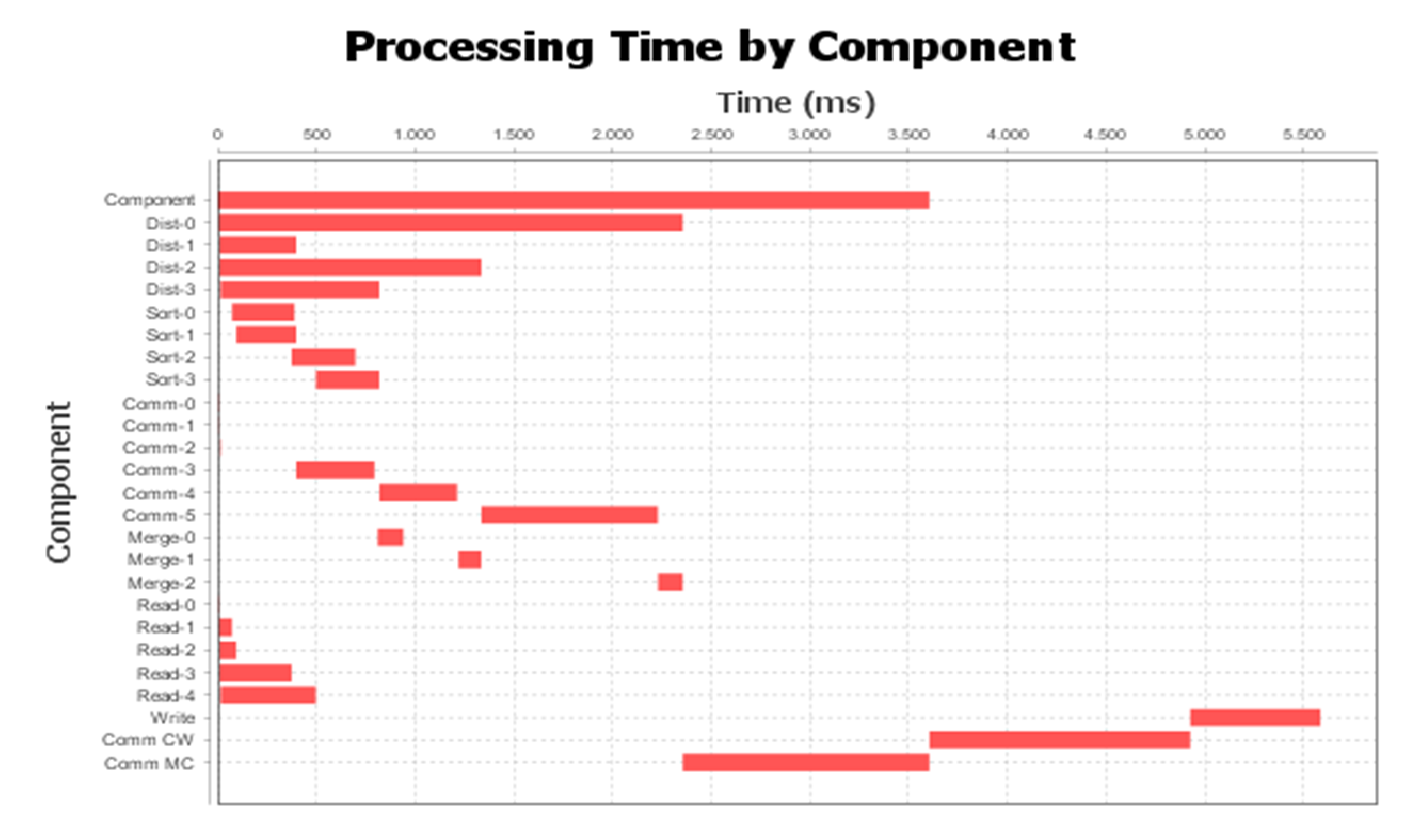
\includegraphics[trim=0.5cm 0cm -5cm 0cm, scale=0.74]{fig/JCUmaRmi498Behavior.eps}
	\caption{Behavior of the JC Sorting Strategy (UMA-RMI)}
	\label{fig:originalStrategyBehaviorRmi}
\end{figure}

First, figure \ref{fig:originalStrategyBehaviorRmi} corresponding to the experiment configured as: 
\begin{itemize}
	\item Communication protocol: RMI.
	\item  Memory structure: Uma.
	\item The number of available nodes: 4
	\item File size: 9'800.0000 Lines.
\end{itemize}
	
Figure \ref{fig:originalStrategyBehaviorRmi} allows to observe how the components interact during their execution (parallel and sequential processes), that is, their behavior. For example, we see that the time described by the chart label "component" has implicit the time corresponding to other components like sorters, mergers, distributors, except the communication time between the Control and the Writer and the writer time, because these components are executed later. The chart allows looking that the distribution phase is executed 4 times (components Dist 0 to Dist 4), one by each processing node. Additionally, we too can observe that the main distributor component-time (Dist 0) has implicit the time corresponding to other components, except the communication time between the merger and the Control components. In the same way figures \ref{fig:originalStrategyBehaviorRest} and \ref{fig:originalStrategyBehaviorIce} show the behavior of this pattern in different configurations.
	
\begin{figure}[H]
	\centering
	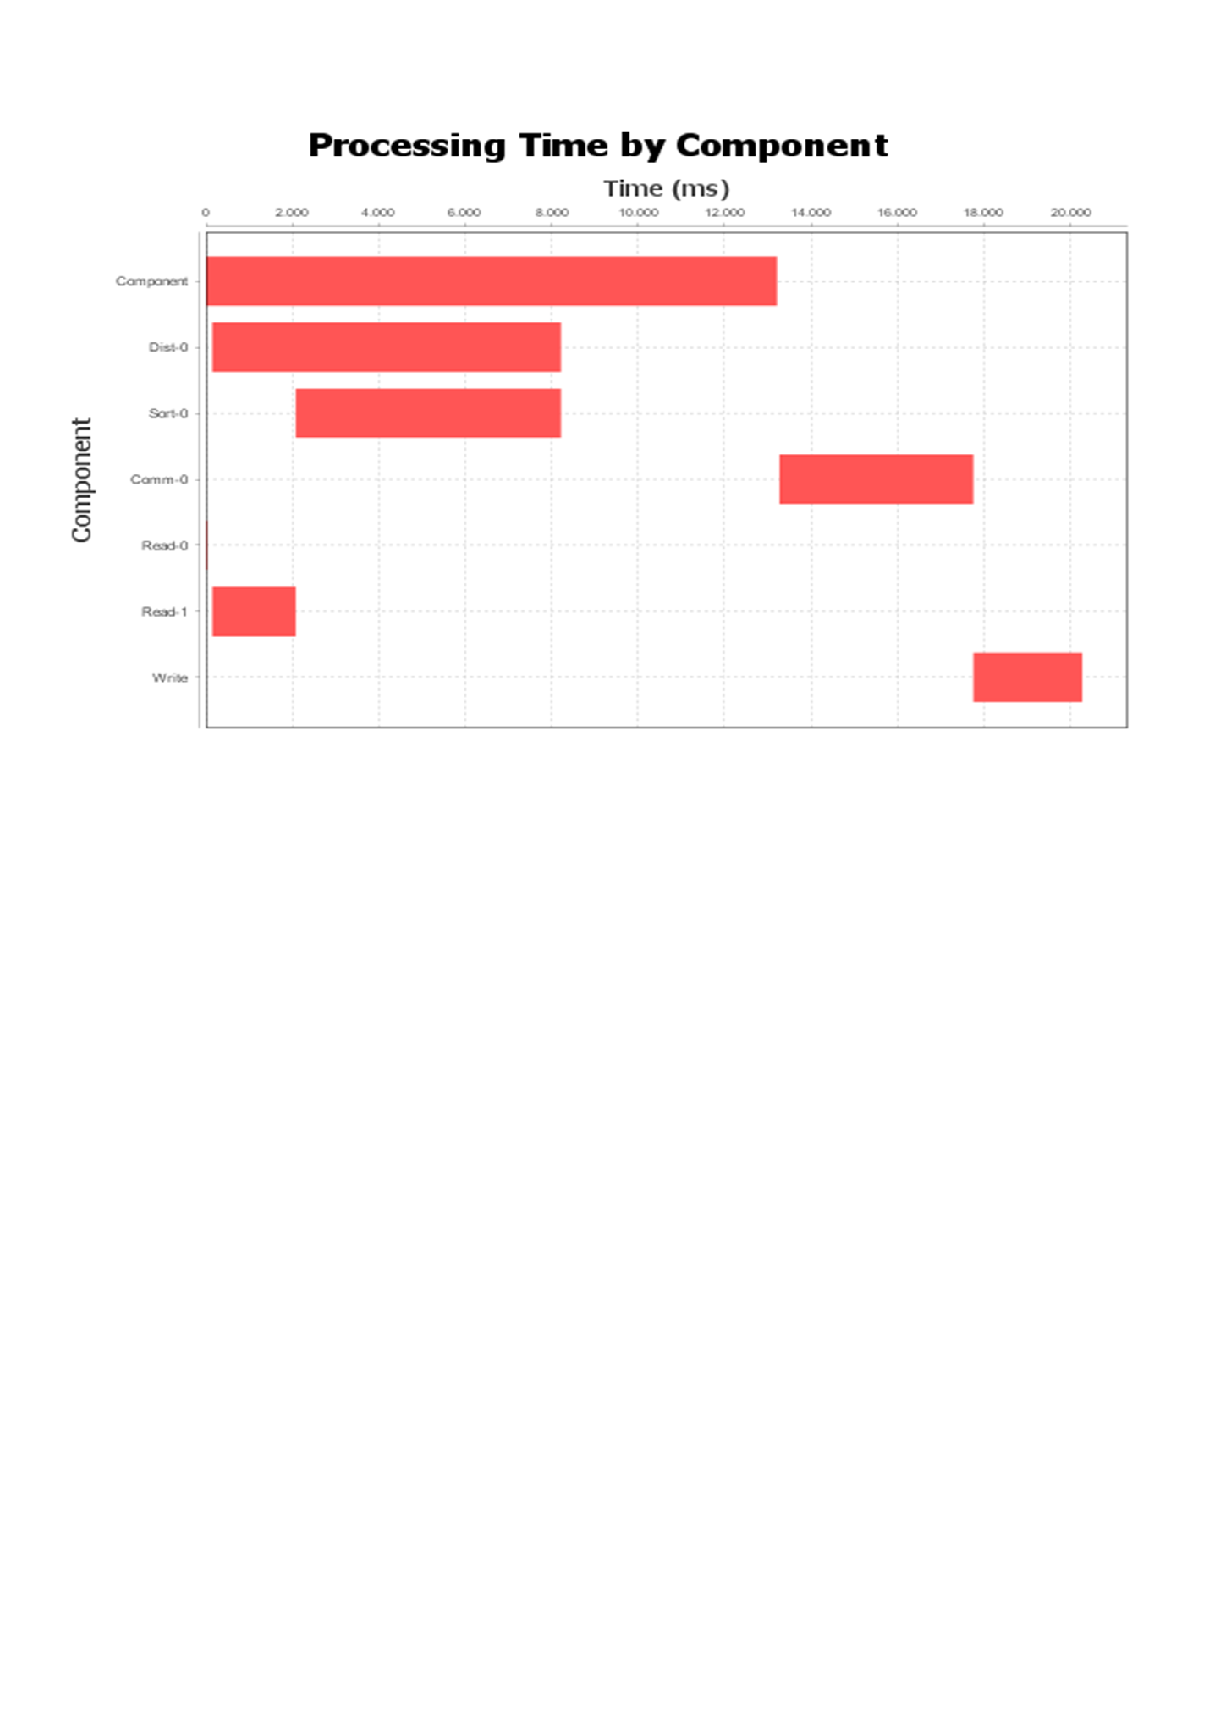
\includegraphics[trim=0.5cm 17cm -5cm 1cm, scale=0.9]{fig/JCUmaRest190Behavior.eps}
	\caption{Behavior of the JC Sorting Strategy (UMA-REST)}
	\label{fig:originalStrategyBehaviorRest}
\end{figure}

Second, figure \ref{fig:originalStrategyBehaviorRest} corresponding to the experiment configured as: 
\begin{itemize}
	\item Communication protocol: REST.
	\item  Memory structure: Uma.
	\item The number of available nodes: 1
 	\item File size: 9'000.0000 Lines.
\end{itemize}

\begin{figure}[H]
	\centering
	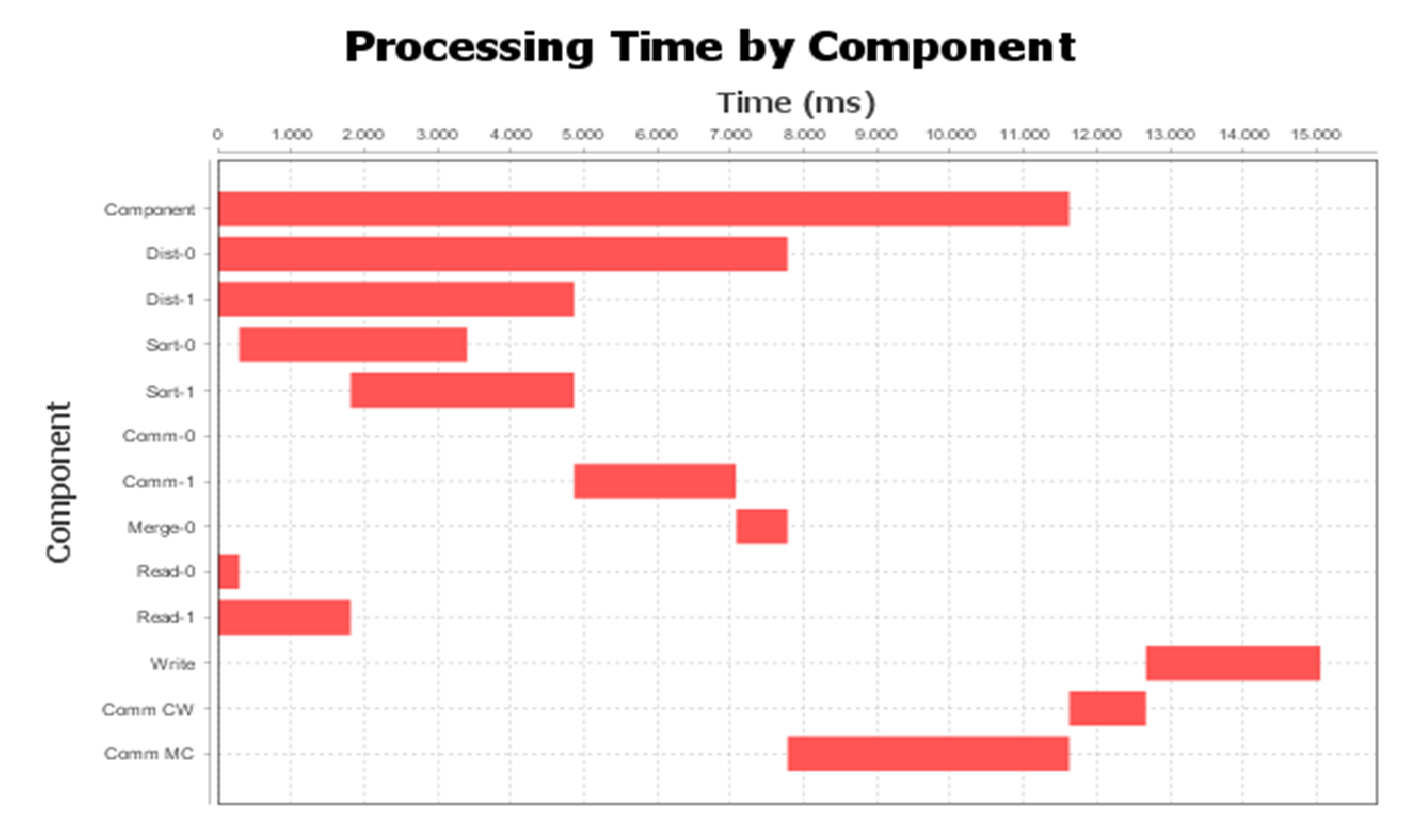
\includegraphics[trim=0.5cm 0cm -5cm 0cm, scale=0.74]{fig/JCUmaIce226Behavior.eps}
	\caption{Behavior of the JC Sorting Strategy (UMA-ICE)}
	\label{fig:originalStrategyBehaviorIce}
\end{figure}

Third, figure \ref{fig:originalStrategyBehaviorIce} corresponding to the experiment configured as: 
\begin{itemize}
	\item Communication protocol: ICE.
	\item  Memory structure: Uma.
	\item The number of available nodes: 2
	\item File size: 2'600.0000 Lines.
\end{itemize}

Throughput all configurations of the JC sorting strategy, we observe that the distribution phase of the main distributor includes, (i) the read phase time, (ii) the sort phase time, (iii) the merge phase time, and (iv) the communication phase time (i.e., the communication time among the distribution components). This is caused because each distributor that makes distribution must wait until all file parts that it distributed returned to it (already sorted) and it can merge them.

The communication phase time above mentioned does not include the communication time between the first distributor and the control component when the sorted file is returned to the control component. Additionally, the communication time between the control component and the writer component when the sorted file is sent to be written is neither included. These times and the communication among the distribution components to return the sorted file to be merged take a huge part of the total time because in the UMA configuration these are the communications with more data traveling through the network.

A particularity of the configuration with 1 available node is that the only one node is responsible to sort the whole file, therefore there is not a merge phase.
\subsection{Analysis of the Behavior of the JC Sorting Strategy Variation }

Figures \ref{fig:variationOriginalStrategyBehaviorIce}, \ref{fig:variationOriginalStrategyBehaviorRest}, and \ref{fig:variationOriginalStrategyBehaviorRmi} show the JC Sorting Strategy variation behavior on different configurations. 

Same that the JC Sorting Strategy, figures \ref{fig:variationOriginalStrategyBehaviorIce}, \ref{fig:variationOriginalStrategyBehaviorRest}, and \ref{fig:variationOriginalStrategyBehaviorRmi} show interaction among components during experiments execution in different configurations. This variation behaves (i.e., the interaction among components and time used by each component) different from the previous due to two main reasons, (i) the merge phase time is not included in the distribution phase time and (ii) the waiting time for the merge is introduced.

\begin{figure}[H]
	\centering
	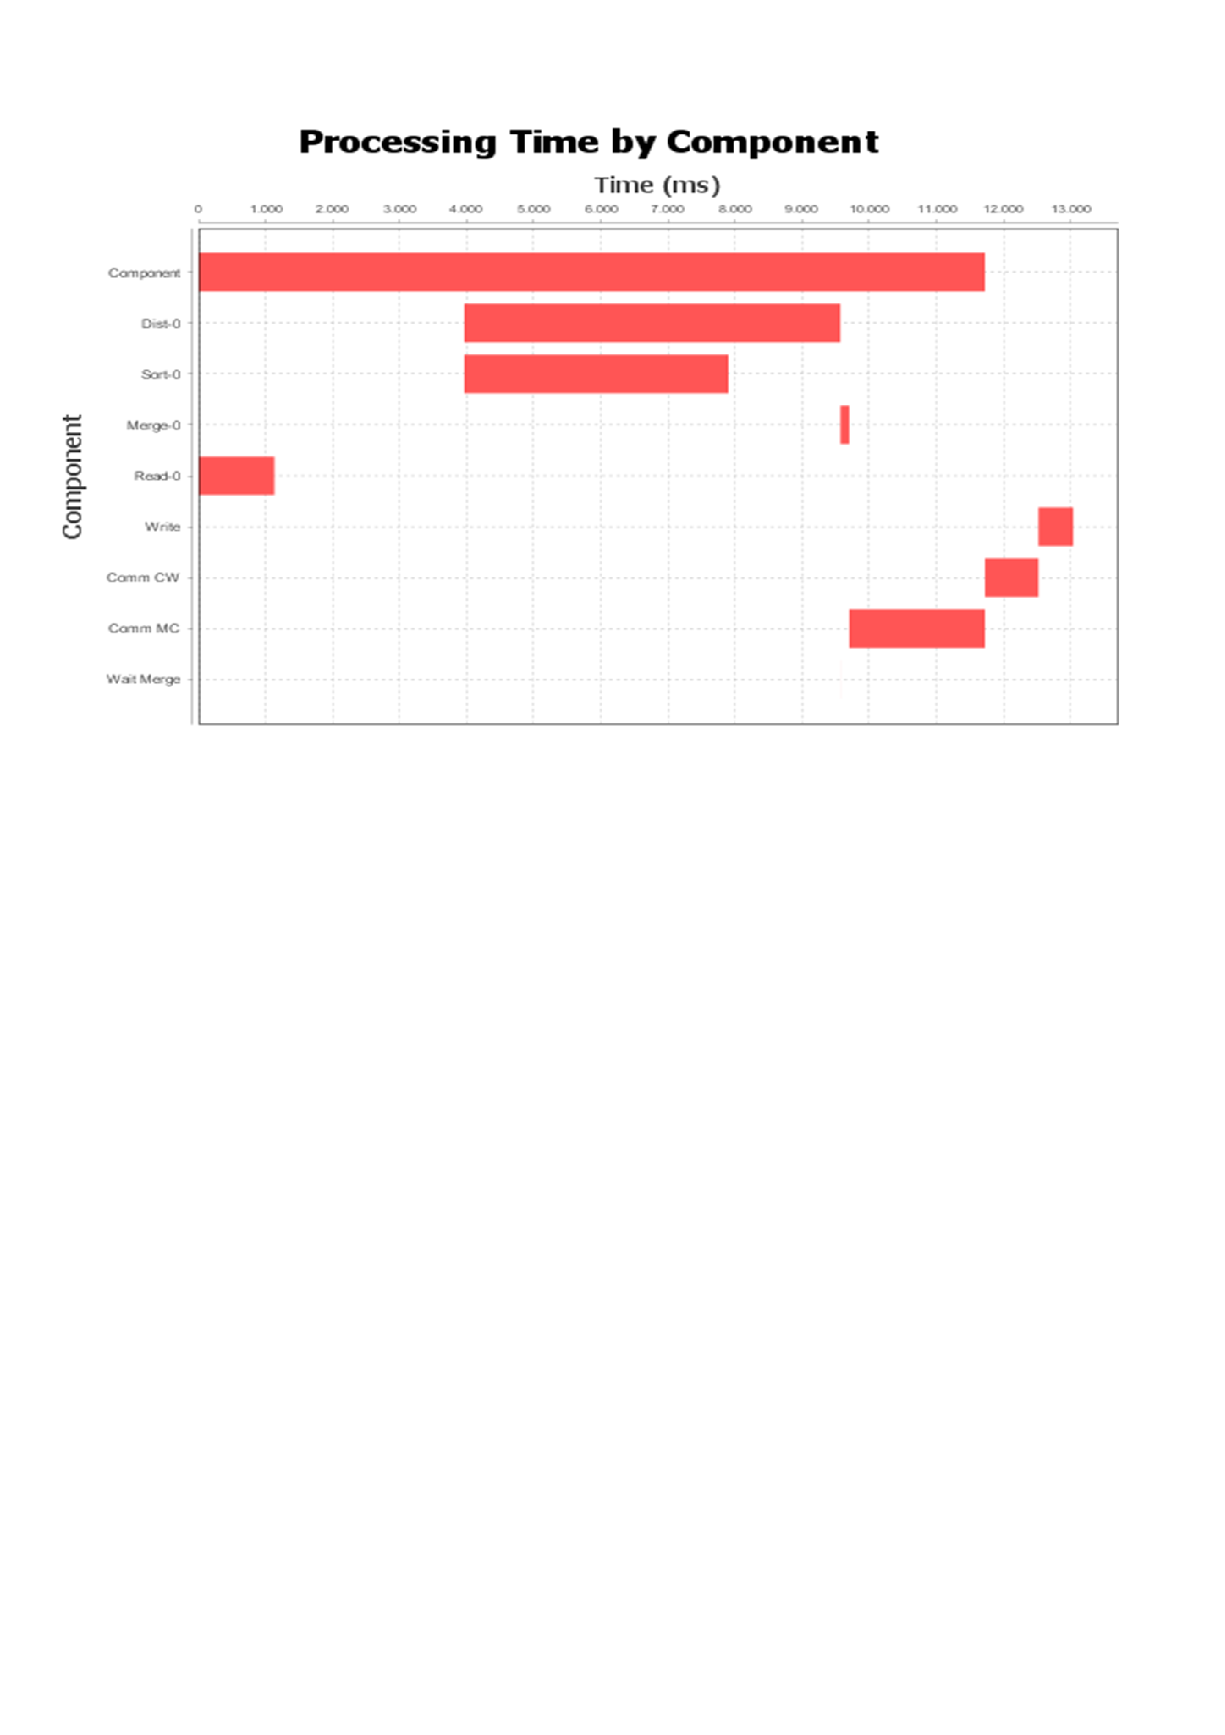
\includegraphics[trim=0.5cm 17cm -5cm 1cm, scale=0.9]{fig/MSNormaIce162Behavior.eps}
	\caption{Behavior of the JC Sorting Strategy Variation (NORMA-ICE)}
	\label{fig:variationOriginalStrategyBehaviorIce}
\end{figure}

First, figure \ref{fig:variationOriginalStrategyBehaviorIce} corresponding to the experiment configured as: 
\begin{itemize}
	\item Communication protocol: ICE.
	\item  Memory structure: Norma.
	\item The number of available nodes: 1
	\item File size: 6'200.0000 Lines.
\end{itemize}

\begin{figure}[H]
	\centering
	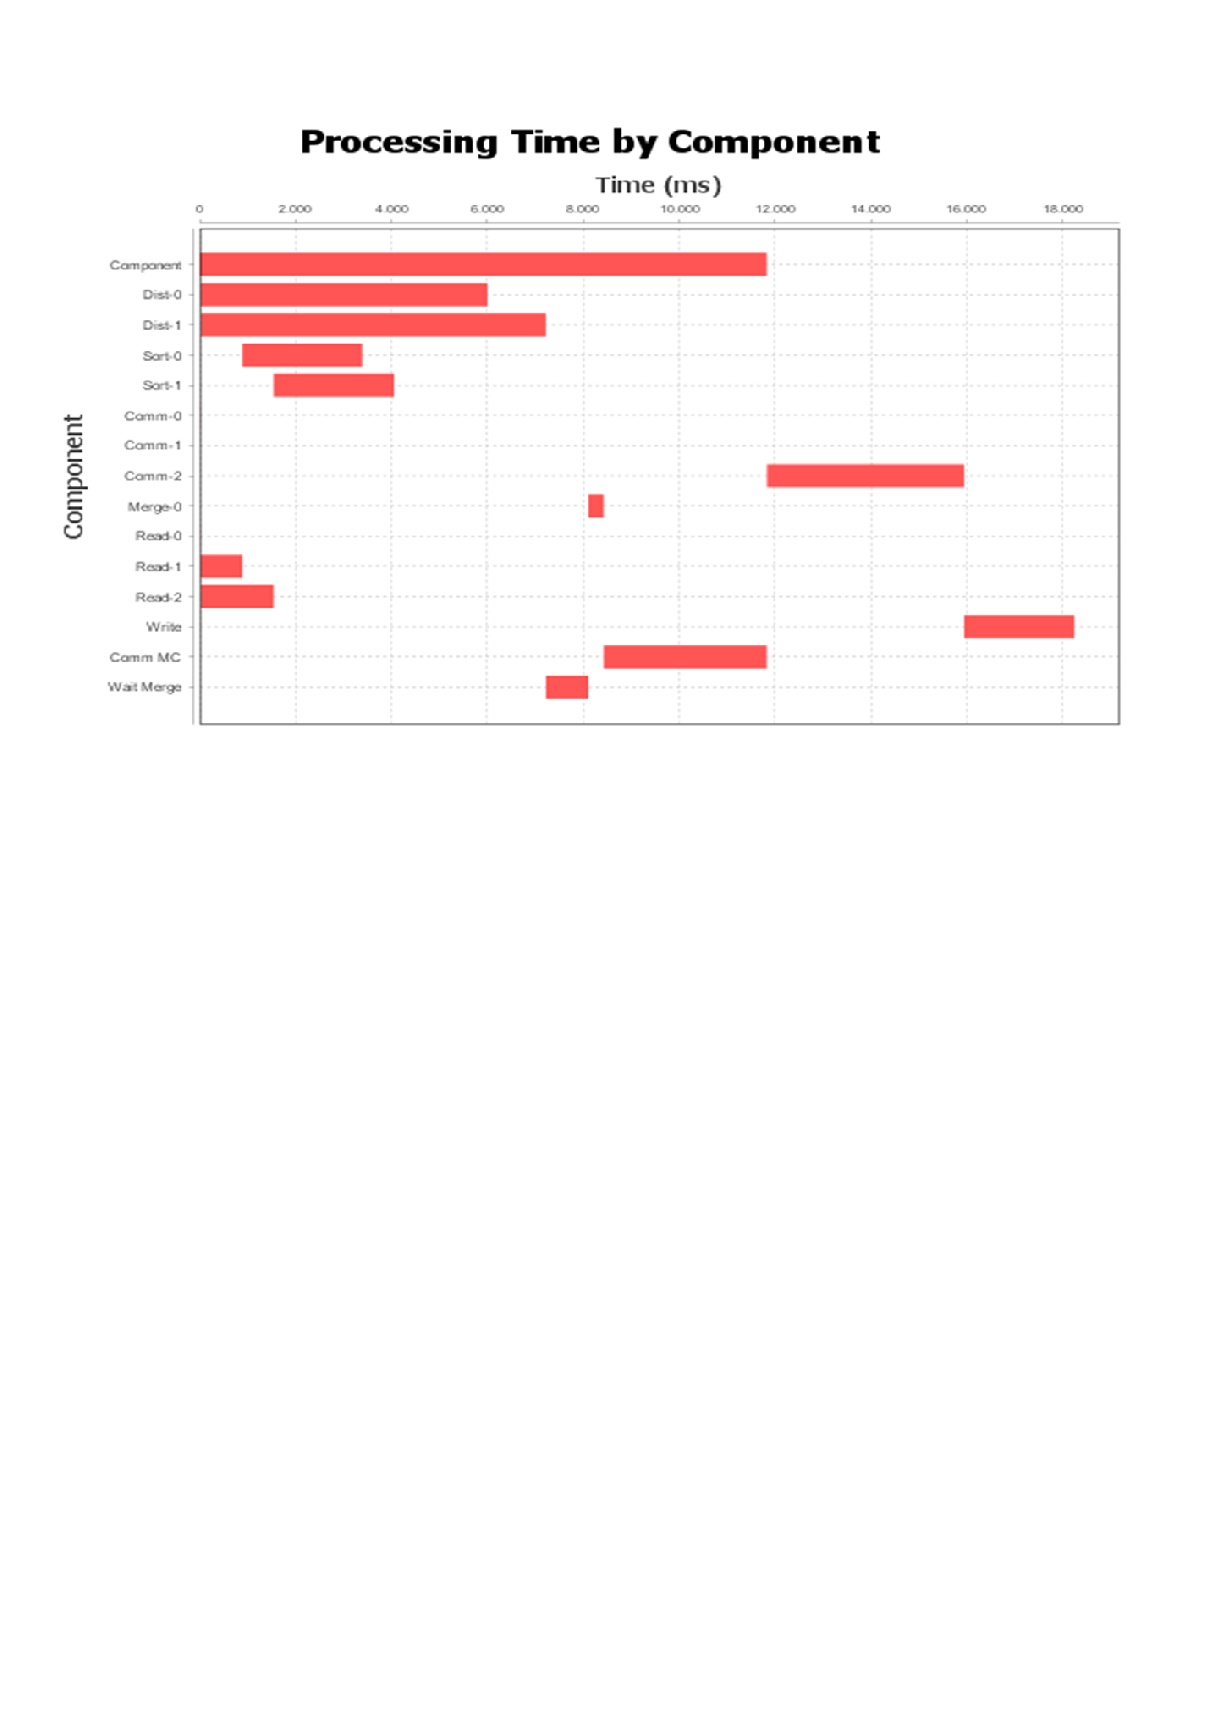
\includegraphics[trim=0.5cm 17cm -5cm 1cm, scale=0.9]{fig/MSUmaRest282Behavior.eps}
	\caption{Behavior of the JC Sorting Strategy Variation (UMA-REST)}
	\label{fig:variationOriginalStrategyBehaviorRest}
\end{figure}

Second,figure \ref{fig:variationOriginalStrategyBehaviorRest} corresponding to the experiment configured as: 
\begin{itemize}
	\item Communication protocol: REST.
	\item  Memory structure: Uma.
	\item The number of available nodes: 2
	\item File size: 8'200.0000 Lines.
\end{itemize}

\begin{figure}[H]
	\centering
	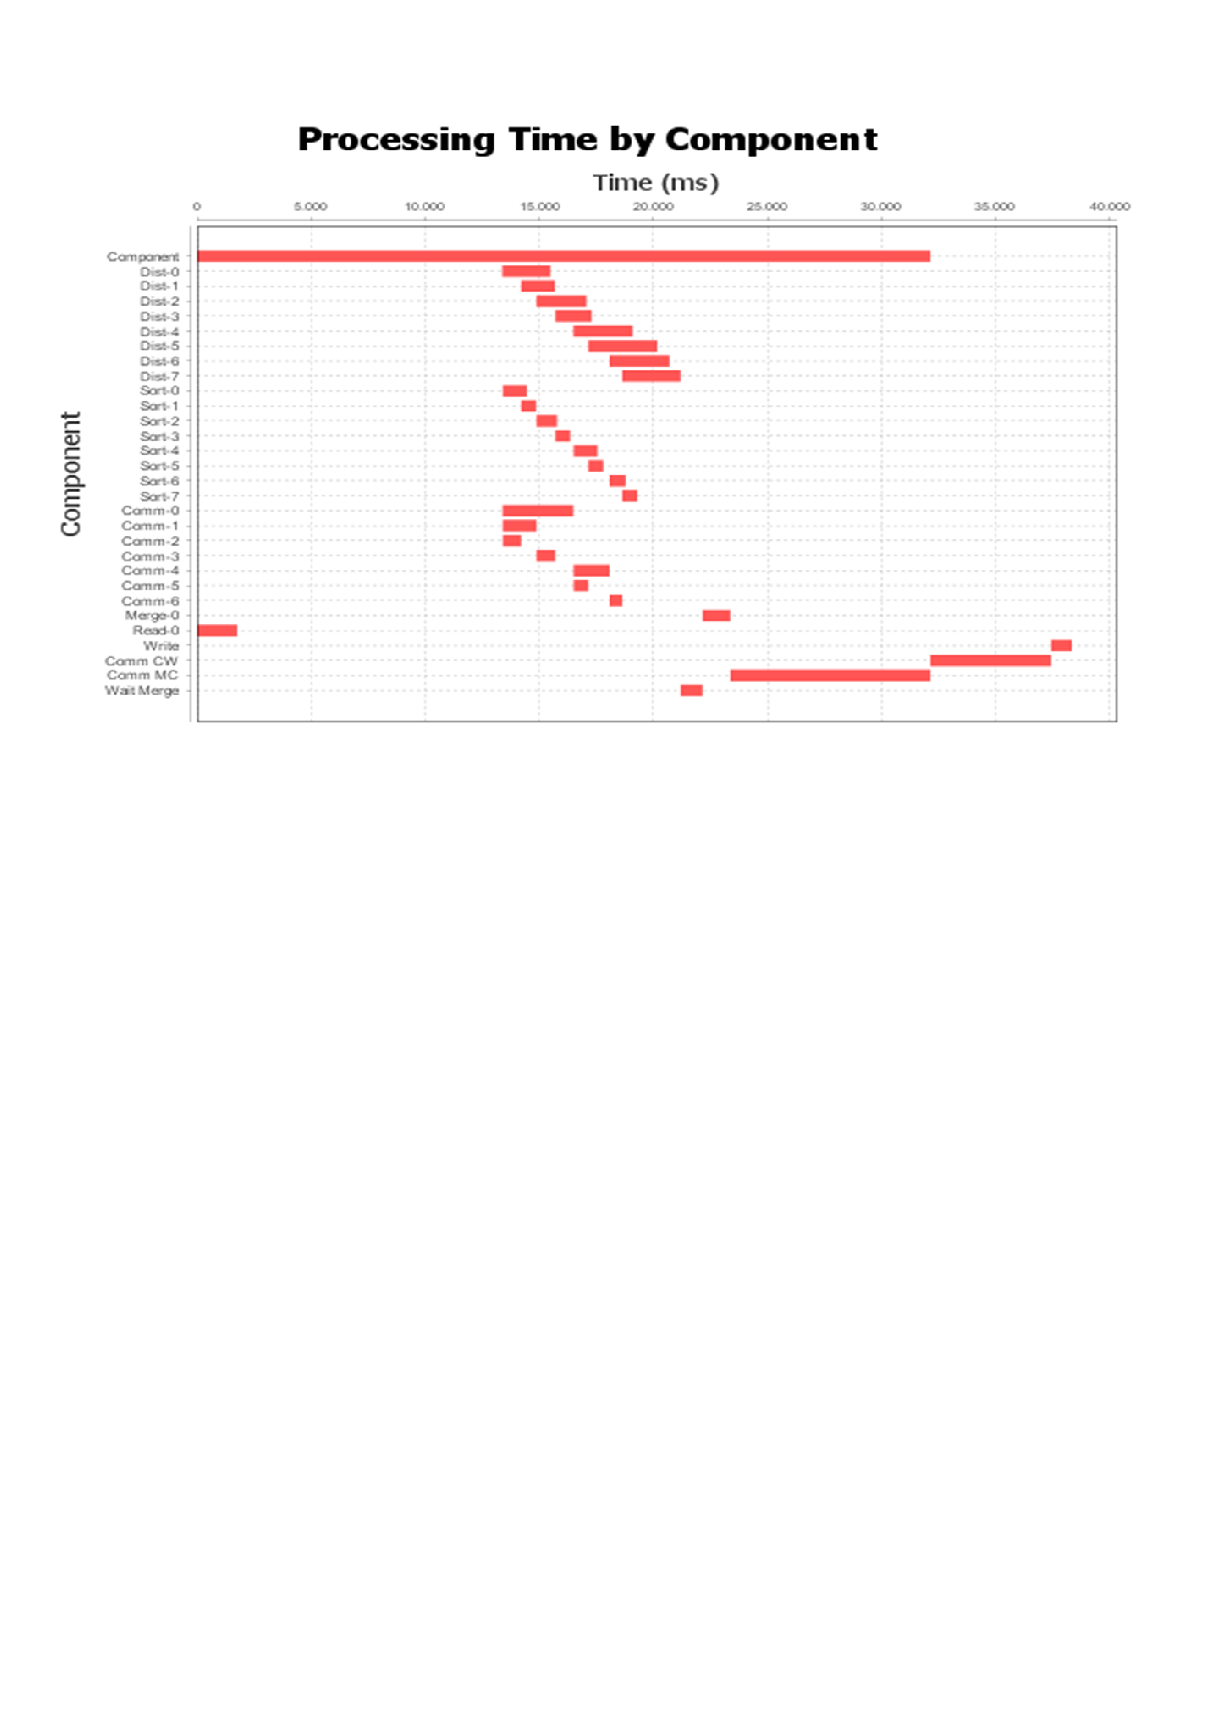
\includegraphics[trim=0.5cm 17cm -5cm 1cm, scale=0.9]{fig/MSNormaRmi890Behavior.eps}
	\caption{Behavior of the JC Sorting Strategy Variation (NORMA-RMI)}
	\label{fig:variationOriginalStrategyBehaviorRmi}
\end{figure}

Third, figure \ref{fig:variationOriginalStrategyBehaviorRmi} corresponding to the experiment configured as: 
\begin{itemize}
	\item Communication protocol: RMI.
	\item  Memory structure: Norma.
	\item The number of available nodes: 8
	\item File size: 9'000.0000 Lines.
\end{itemize}


The NORMA configurations show a time that was not measured in the first experiments, this can be observed in figures \ref{fig:variationOriginalStrategyBehaviorIce} and \ref{fig:variationOriginalStrategyBehaviorRmi}. These figures show that between the read component measured time and the first distributor component measured time, there is a considerable time that was unknown its source. In posterior experiments, new measures were introduced and then we discover that the unknown time corresponds to the communication time between the read component and the control component when the file to be sorted is read and loaded to memory. In addition, the communication time when the control component sends the read file to the main distributor. These measures suggest that despite the components are located in the same node, the communication time among these components is not depreciable.

Another time that was not measured is the time to send the sorted file part from the sort component to the merge component, this time can be observed as the time from end the sort phase time until the end of the distribution phase time. 

Because the file to be sorted should travel from one component to other, therefore, we conclude that when we are in a distributed environment an important key is to keep the communication time as small as to be possibly among processing nodes and among components in the same processing node too.

%\newpage

\subsection{Analysis of the Behavior of the Fork/Join Java Library Variation }

The figures \ref{fig:forkJoinLibraryBehaviorIce}, \ref{fig:forkJoinLibraryBehaviorRest}, and \ref{fig:forkJoinLibraryBehaviorRmi} show the Fork/Join Java library variation behavior on different configurations. 

\begin{figure}[H]
	\centering
	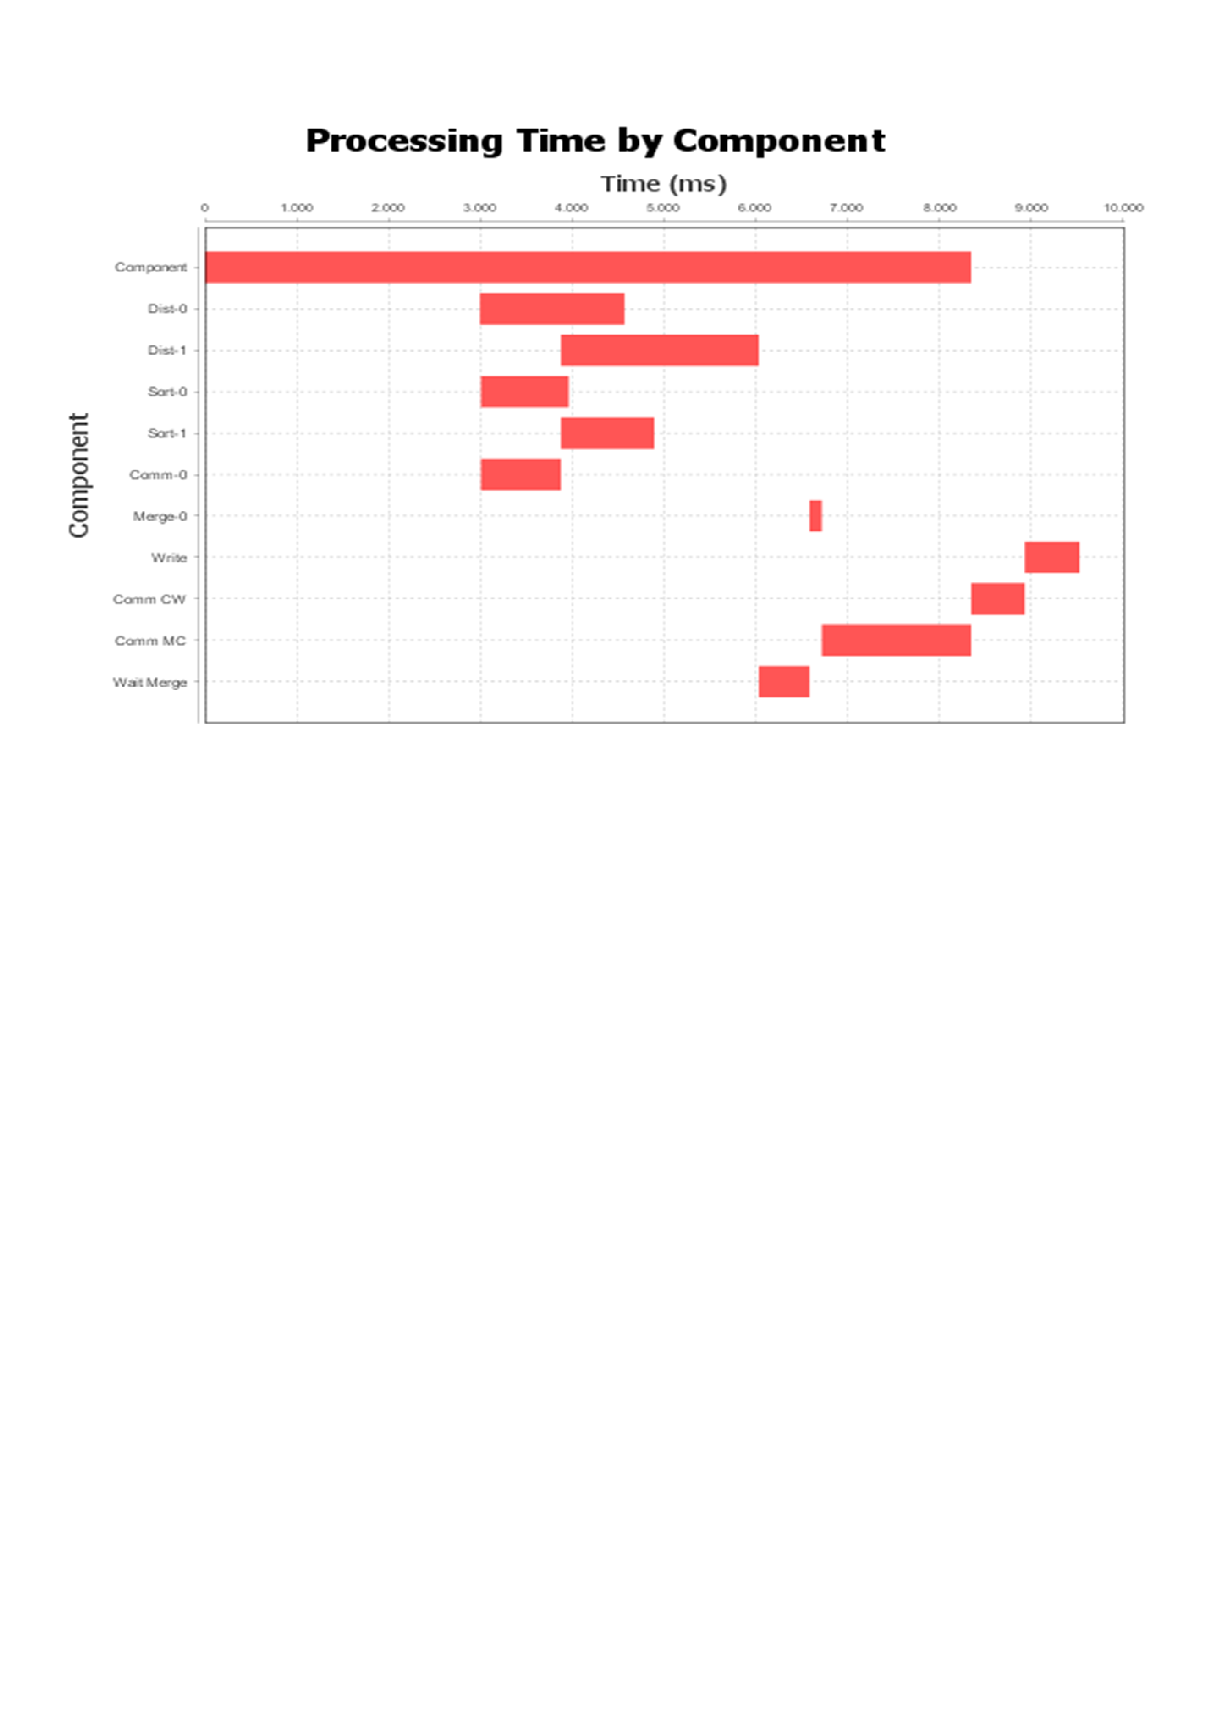
\includegraphics[trim=0.5cm 17cm -5cm 1cm, scale=0.9]{fig/FJNormaIce250Behavior.eps}
	\caption{Behavior of the Fork/Join Java Library Variation (NORMA-ICE)}
	\label{fig:forkJoinLibraryBehaviorIce}
\end{figure}
First, figure \ref{fig:forkJoinLibraryBehaviorIce} corresponding to the experiment configured as: 
\begin{itemize}
	\item Communication protocol: ICE.
	\item  Memory structure: Norma.
	\item The number of available nodes: 2
	\item File size: 5'000.0000 Lines.
\end{itemize}

\begin{figure}[H]
	\centering
	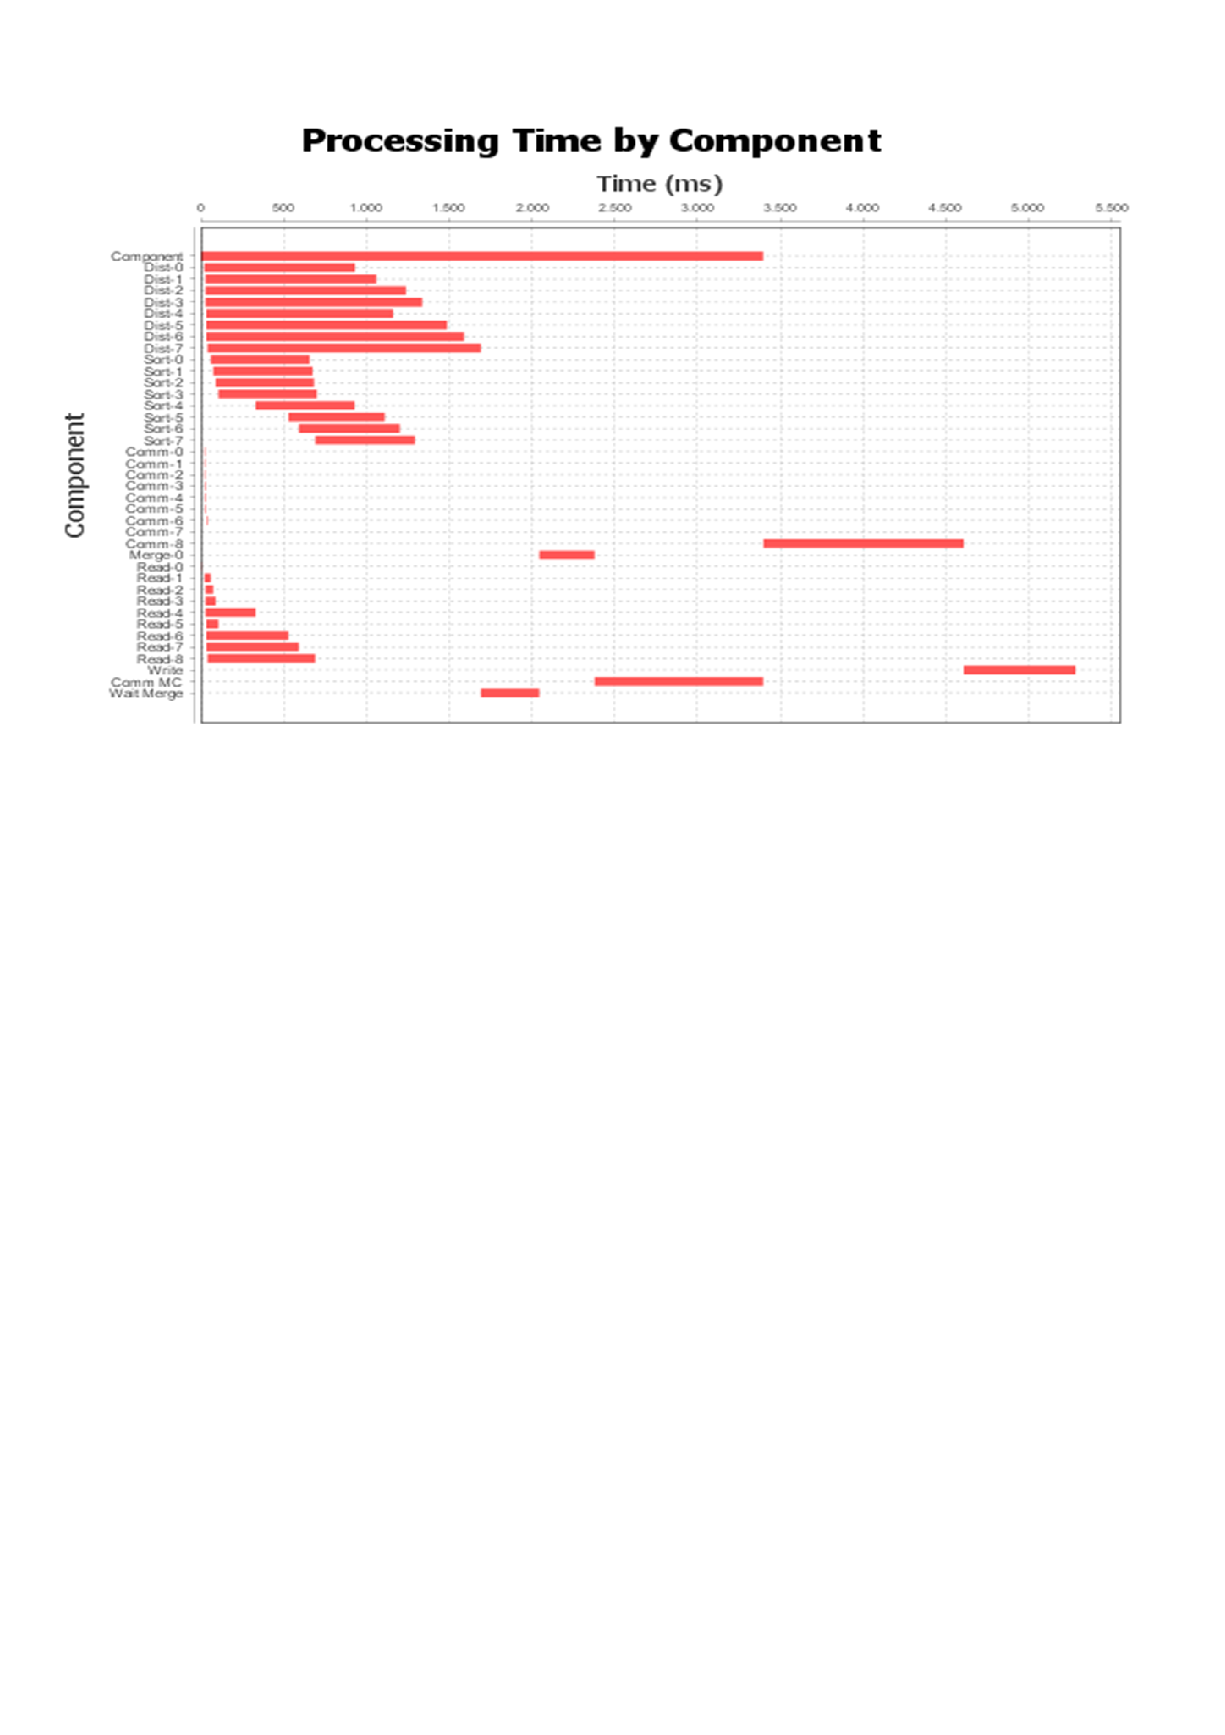
\includegraphics[trim=0.5cm 17cm -5cm 1cm, scale=0.9]{fig/FJUmaRest826Behavior.eps}
	\caption{Behavior of the Fork/Join Java Library Variation (UMA-REST)}
	\label{fig:forkJoinLibraryBehaviorRest}
\end{figure}
Second, figure \ref{fig:forkJoinLibraryBehaviorRest} corresponding to the experiment configured as: 
\begin{itemize}
	\item Communication protocol: REST.
	\item  Memory structure: Uma.
	\item The number of available nodes: 8
	\item File size: 2'600.0000 Lines.
\end{itemize}

In UMA configurations the distribution phase includes the read and sort phases, first, the read phase is executed and then the sort phase can be executed. We can observe that the read phase has specific behavior with UMA, all distribution and read phases start almost at the same time, however, despite each reading phase reads the same size of different file parts, each read can take a different time amount. This situation shows the UMA limitations when many components try to access the memory, we can observe in figures \ref{fig:variationOriginalStrategyBehaviorRest} and \ref{fig:forkJoinLibraryBehaviorRest} that between more read phases, the time to read the same file size has more variation. This causes that the sort phase starts at different times and each distribution phase uses a different amount of time to sort the different file parts with the same size.

\begin{figure}[H]
	\centering
	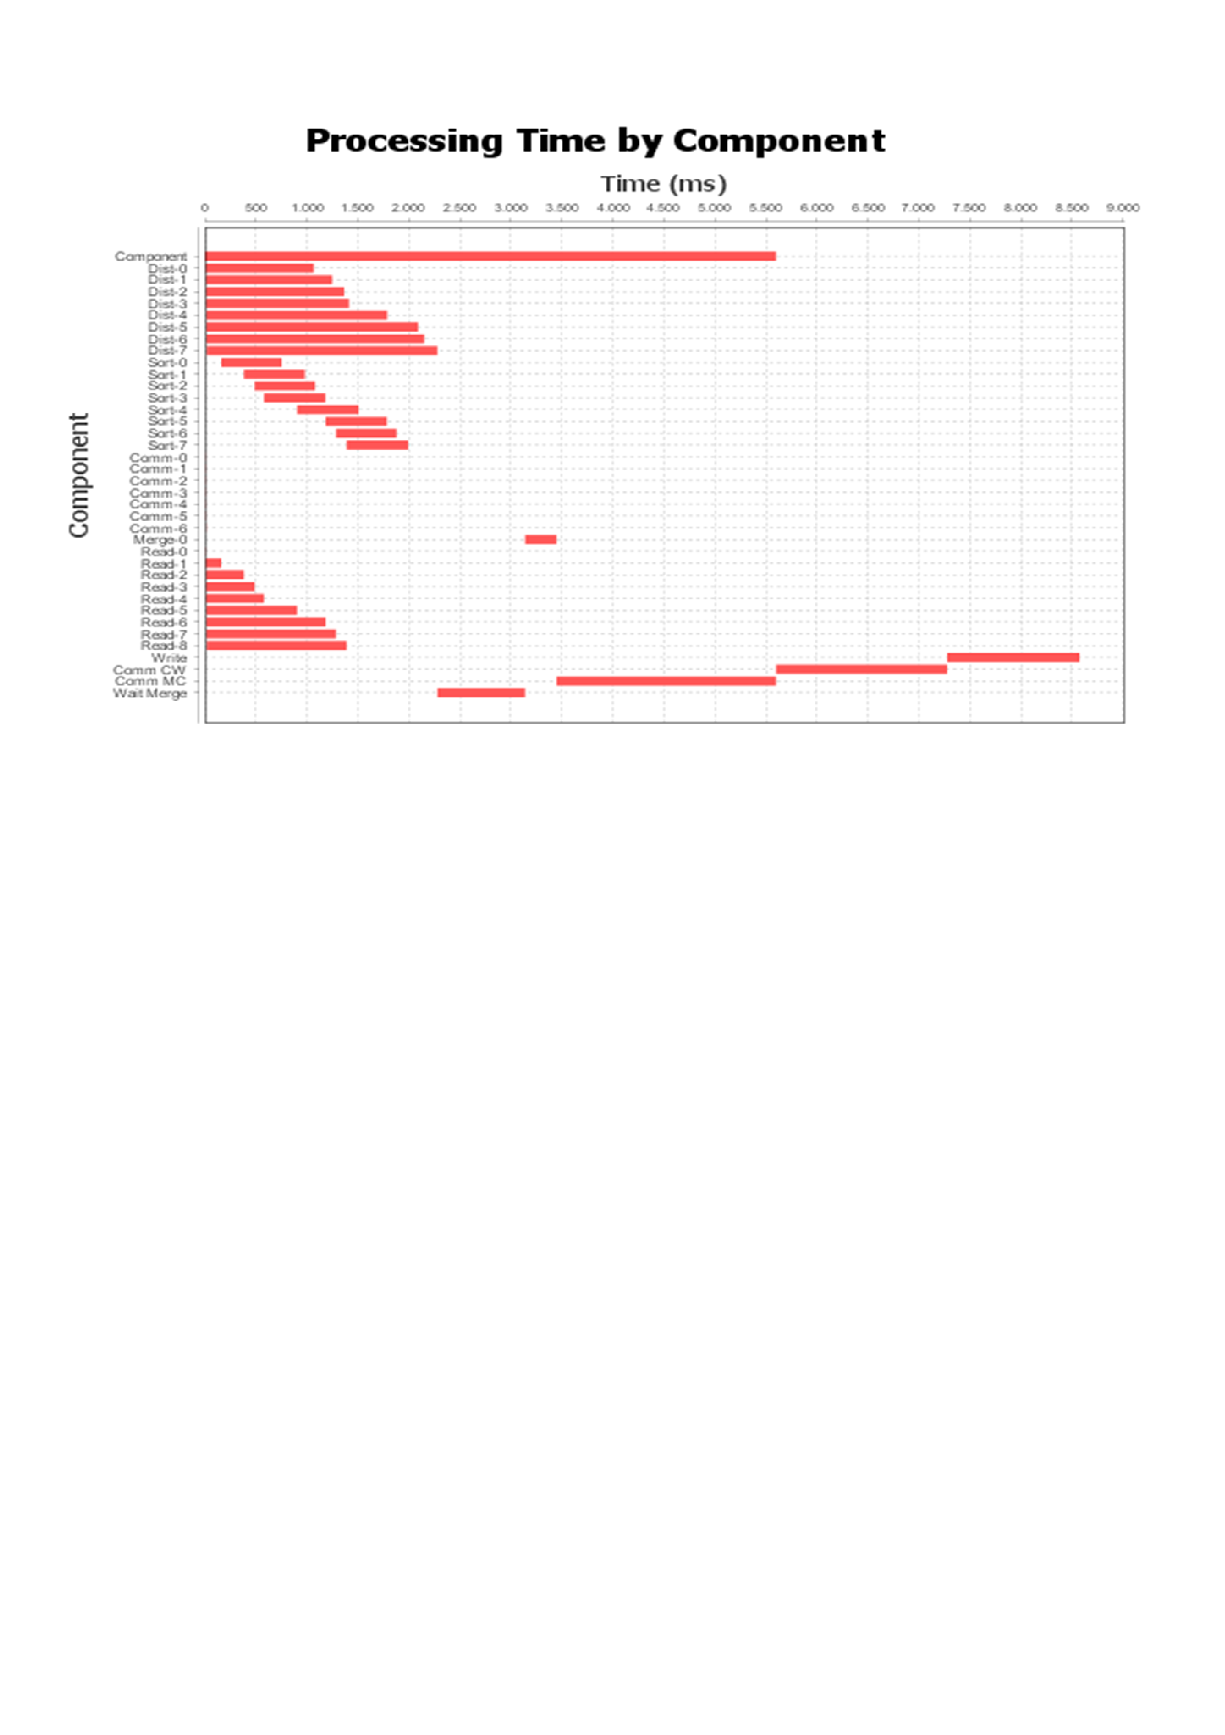
\includegraphics[trim=0.5cm 17cm -5cm 1cm, scale=0.9]{fig/FJUmaRmi842Behavior.eps}
	\caption{Behavior of the Fork/Join Java Library Variation (UMA-RMI)}
	\label{fig:forkJoinLibraryBehaviorRmi}
\end{figure}
Third,figure \ref{fig:forkJoinLibraryBehaviorRmi} corresponding to the experiment configured as: 
\begin{itemize}
	\item Communication protocol: RMI.
	\item  Memory structure: Uma.
	\item The number of available nodes: 8
	\item File size: 4'200.0000 Lines.
\end{itemize}

This variation has the same behavior as the JC Sorting Strategy variation, that is, the changes in the behavior is not observed through the figures \ref{fig:forkJoinLibraryBehaviorIce}, \ref{fig:forkJoinLibraryBehaviorRest}, and \ref{fig:forkJoinLibraryBehaviorRmi}, because the main change is in how the CPU cores are used. Including the interaction among components in the NORMA and UMA configurations. Each sort phase uses the fork / join Java library. To use this library implies to determine a threshold until the item to be processed is forked. We define the threshold according to the CPU use percentage of each node's CPUs and the part file to be sorted. If the CPU use percentage of one CPU core is less than 40\%, it is a candidate to be used. However, the operating system is responsible for finally assigning work to each CPU core. The threshold was calculated as the part file length divided on the CPU core amount that could be used.

\subsection{Analysis of the Behavior of the Fork-Join Design Pattern }

Figures \ref{fig:forkJoinBehaviorIce}, \ref{fig:forkJoinBehaviorRest}, and \ref{fig:forkJoinBehaviorRmi} show the Fork/Join design pattern behavior on different configurations. 

\begin{figure}[H]
	\centering
	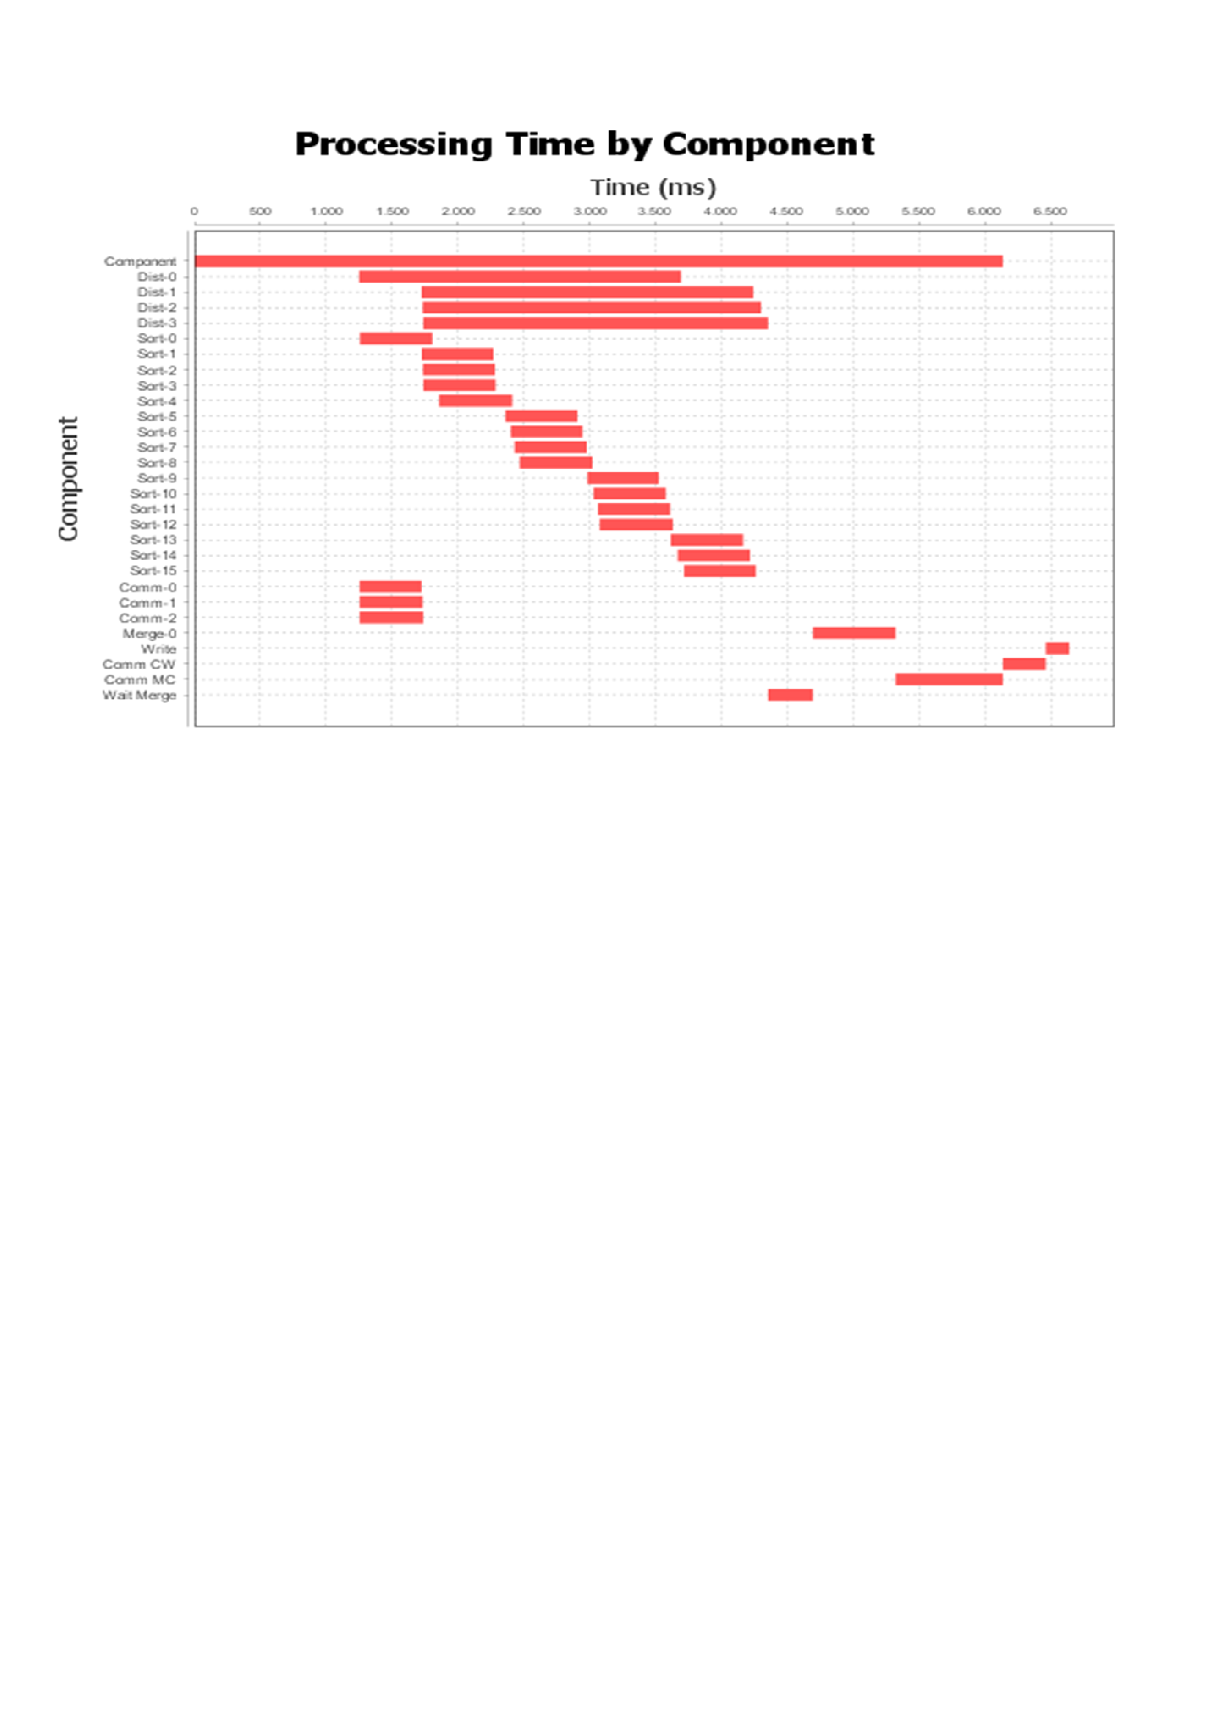
\includegraphics[trim=0.5cm 17cm -5cm 1cm, scale=0.9]{fig/FJDNormaIce426Behavior.eps}
	\caption{Behavior of the Fork-Join Design Pattern (NORMA-ICE)}
	\label{fig:forkJoinBehaviorIce}
\end{figure}

First, figure \ref{fig:forkJoinBehaviorIce} corresponding to the experiment configured as: 
\begin{itemize}
	\item Communication protocol: ICE.
	\item  Memory structure: Norma.
	\item The number of available nodes: 4
	\item File size: 2'600.0000 Lines.
\end{itemize}

This design pattern has a behavior very different from the above strategies, figure \ref{fig:forkJoinBehaviorIce} shows that there are only four distribution phases, one for each processing node, but there are 16 sort phases, four for each distribution phase. This behavior is caused by all processing nodes divides their own file part waiting that their children help to process if children finish processing before its parent. The times used to process in each processing node are very similar, unlike the above strategies.

\begin{figure}[H]
	\centering
	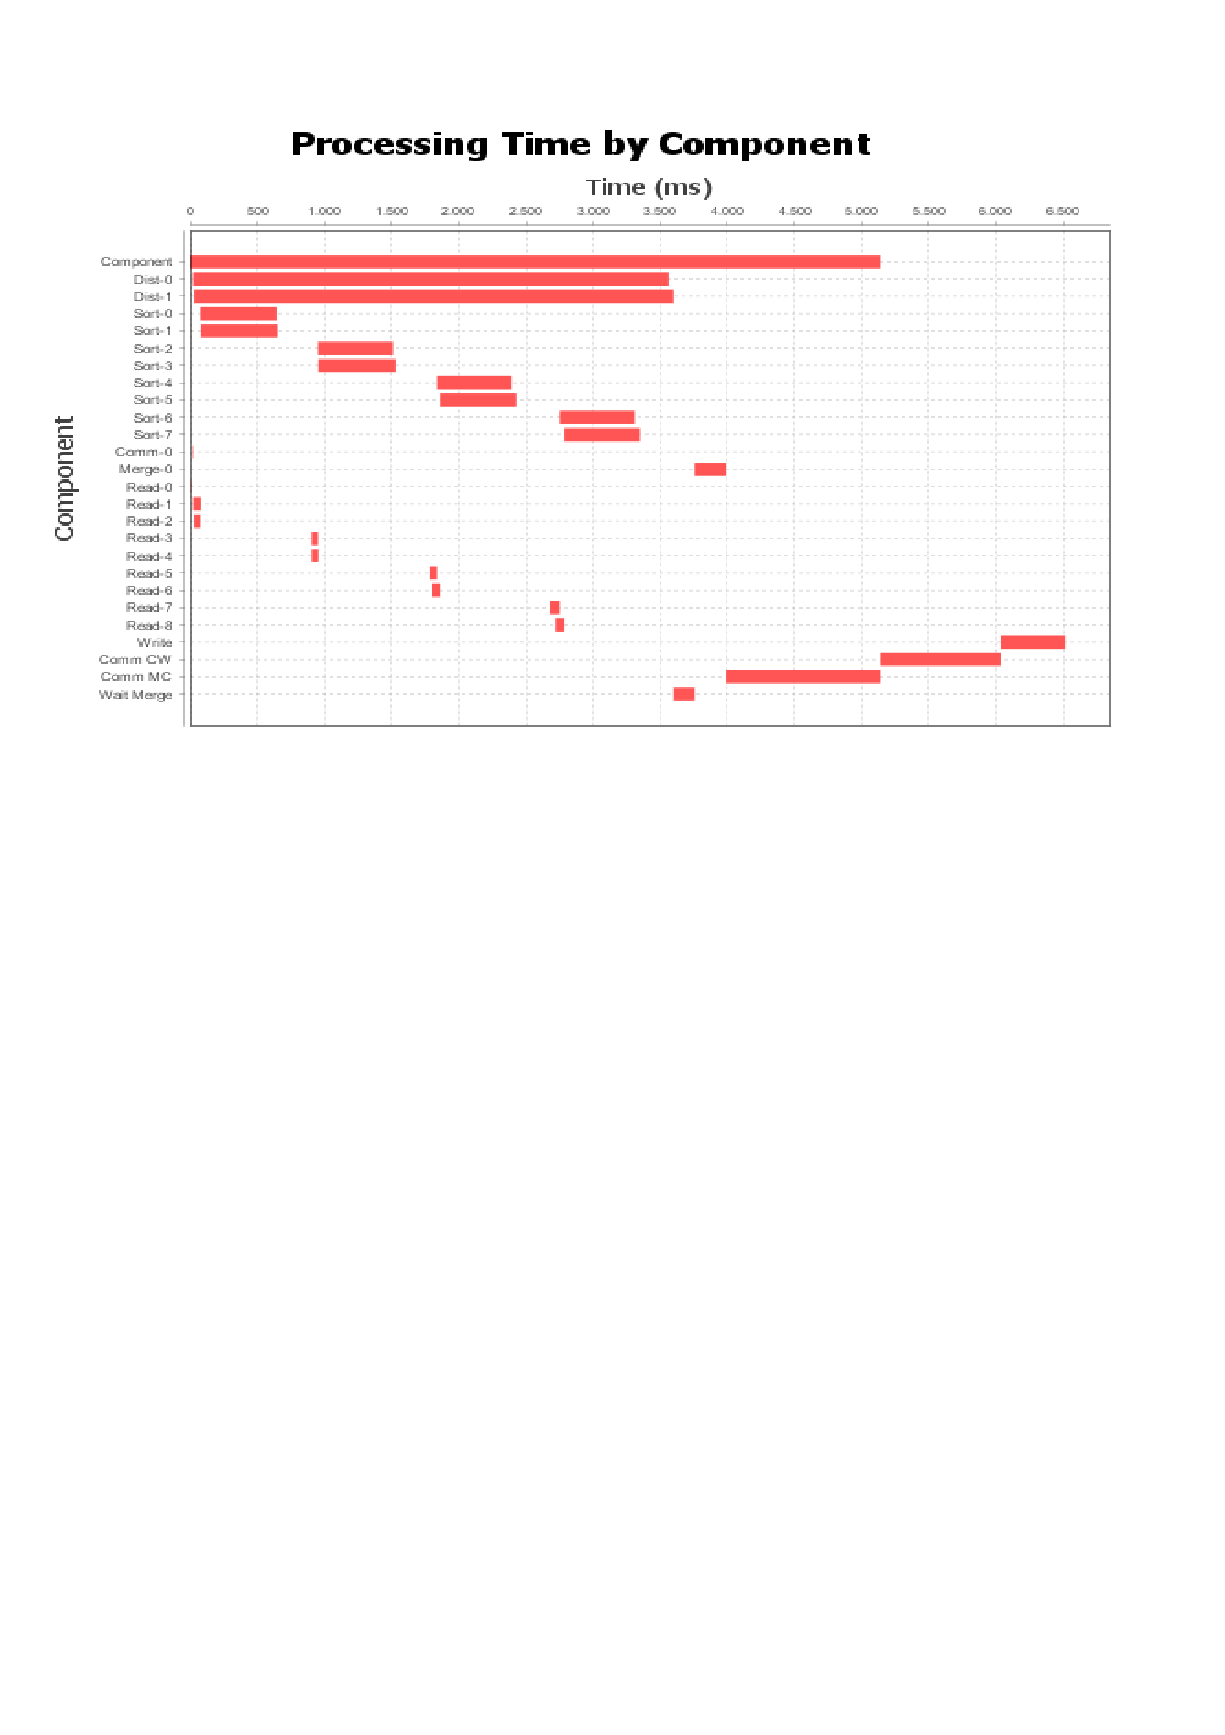
\includegraphics[trim=0.5cm 17cm -5cm 1cm, scale=0.9]{fig/FJDUmaRest218Behavior.eps}
	\caption{Behavior of the Fork-Join Design Pattern (UMA-REST)}
	\label{fig:forkJoinBehaviorRest}
\end{figure}
Second, figure \ref{fig:forkJoinBehaviorRest} corresponding to the experiment configured as: 
\begin{itemize}
	\item Communication protocol: REST.
	\item  Memory structure: Uma.
	\item The number of available nodes: 2
	\item File size: 1'800.0000 Lines.
\end{itemize}

This pattern shows the same behavior detected in the interaction among components in the NORMA and UMA configurations in above strategies.

\begin{figure}[H]
	\centering
	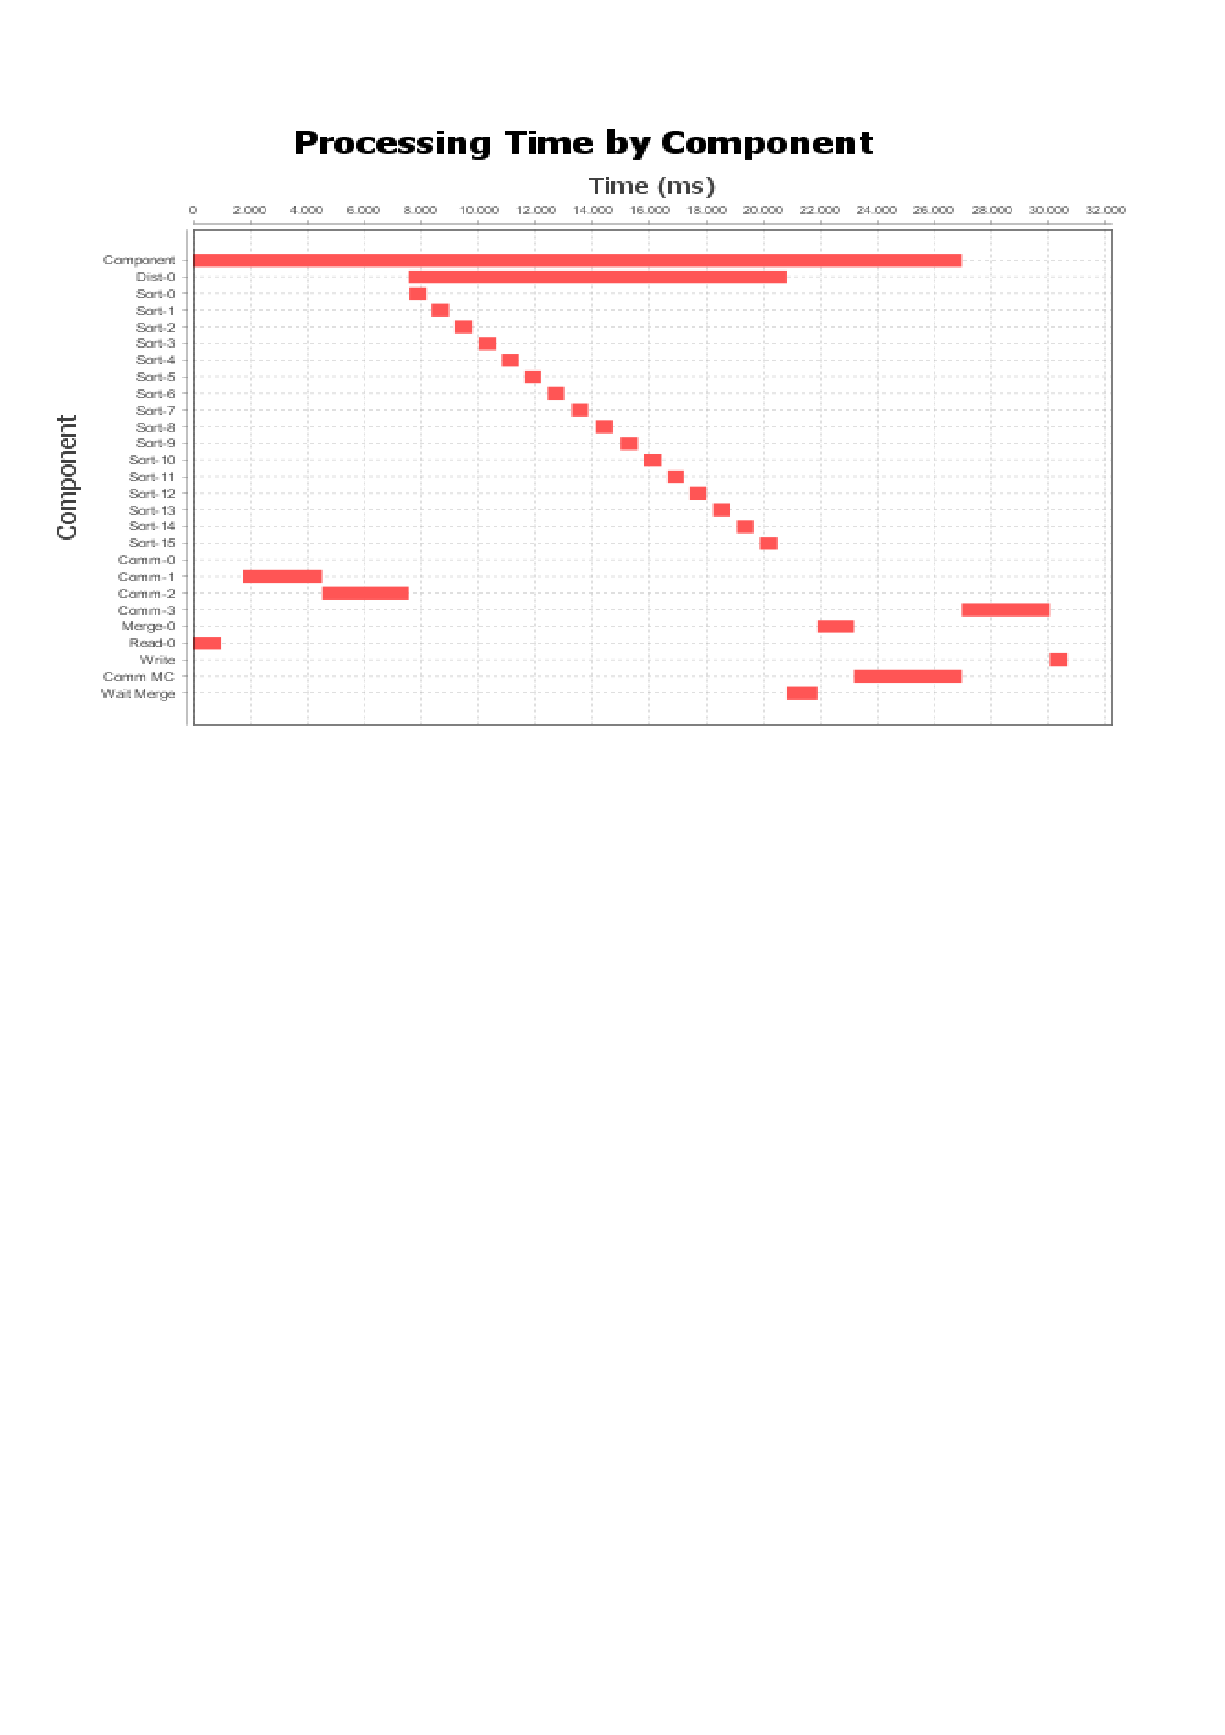
\includegraphics[trim=0.5cm 17cm -5cm 1cm, scale=0.9]{fig/FJDNormaRmi154Behavior.eps}
	\caption{Behavior of the Fork-Join Design Pattern (NORMA-RMI)}
	\label{fig:forkJoinBehaviorRmi}
\end{figure}
Third, figure \ref{fig:forkJoinBehaviorRmi} corresponding to the experiment configured as: 
\begin{itemize}
	\item Communication protocol: RMI.
	\item  Memory structure: Norma.
	\item The number of available nodes: 1
	\item File size: 5'400.0000 Lines.
\end{itemize}

In figure \ref{fig:forkJoinBehaviorRmi} we can observe that only one processing node is configured and 16 sort phases are executed the same that in figure \ref{fig:forkJoinBehaviorIce}, this is caused because the sort phases amount is not dependent of processing nodes amount, else it depends on the file size.

This design pattern tries to distribute in a homogeneous way, that is, all nodes can have the same nodes number of children. This is an important difference to the JC Sorting Strategy and it causes a completely different behavior. First, the file to be sorted is split considering not only the number available nodes but also the minimum file size to leverage distribution. The minimum file size was configured as 400.000 lines, as determined by preparatory experiments. 

Each node splits the file to be sorted and sends all parts (including its own part)  to be sorted at the same time. This is the first difference that we can observe between figures \ref{fig:forkJoinBehaviorIce} and \ref{fig:forkJoinBehaviorRest}. The time for the distribution phase is very similar at the same level, where a level represents how many processing nodes are located before hierarchically, for example, the first father is located in the "n" level and all its children are located in the "n-1" level. For example, in figure \ref{fig:forkJoinBehaviorIce}, Dist0 corresponding to a superior level, but Dist1, Dist2, and Dist3 are very similar given that they are at the same level.

The second difference is observed in the sort phase. Each node recursively divides its own file part into halves while the file part is bigger than the minimum file size to distribute and it sends each half to the queue. Then, each node sorts the file parts in the queue. The queue allows that if a child node finishes its processes before its father node, it can take work of the father queue. To sort each queue item, this variation uses the fork / join Java library.

This design pattern shows the same difference between the UMA and NORMA configurations detected in the JC Sorting Strategy Variation.

\subsection{Analysis of the Behavior of the Leader-Followers Design Pattern }

\begin{figure}[H]
	\centering
	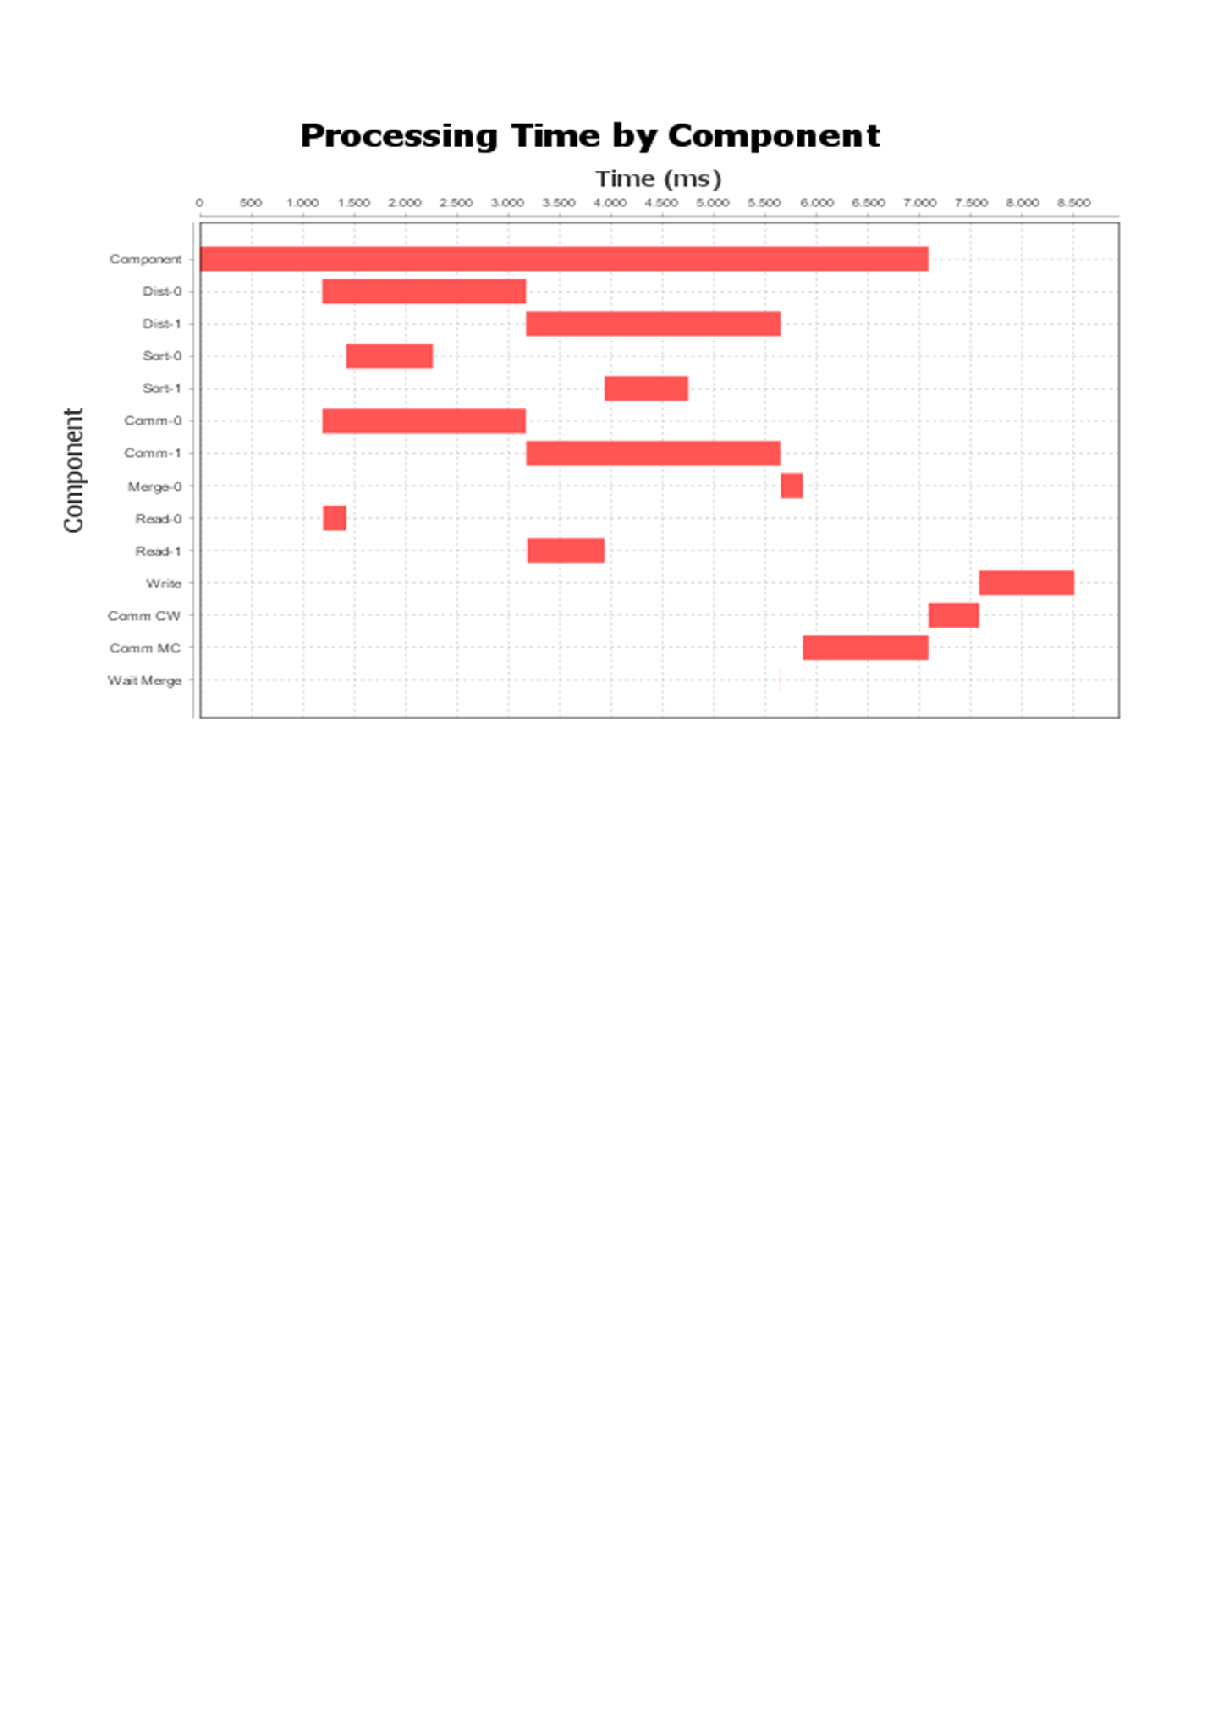
\includegraphics[trim=0.5cm 17cm -5cm 1cm, scale=0.9]{fig/LFUmaIce438Behavior.eps}
	\caption{Behavior of the Leader-Followers Design Pattern (UMA-ICE)}
	\label{fig:leaderFollowersBehaviorIce}
\end{figure}

\begin{figure}[H]
	\centering
	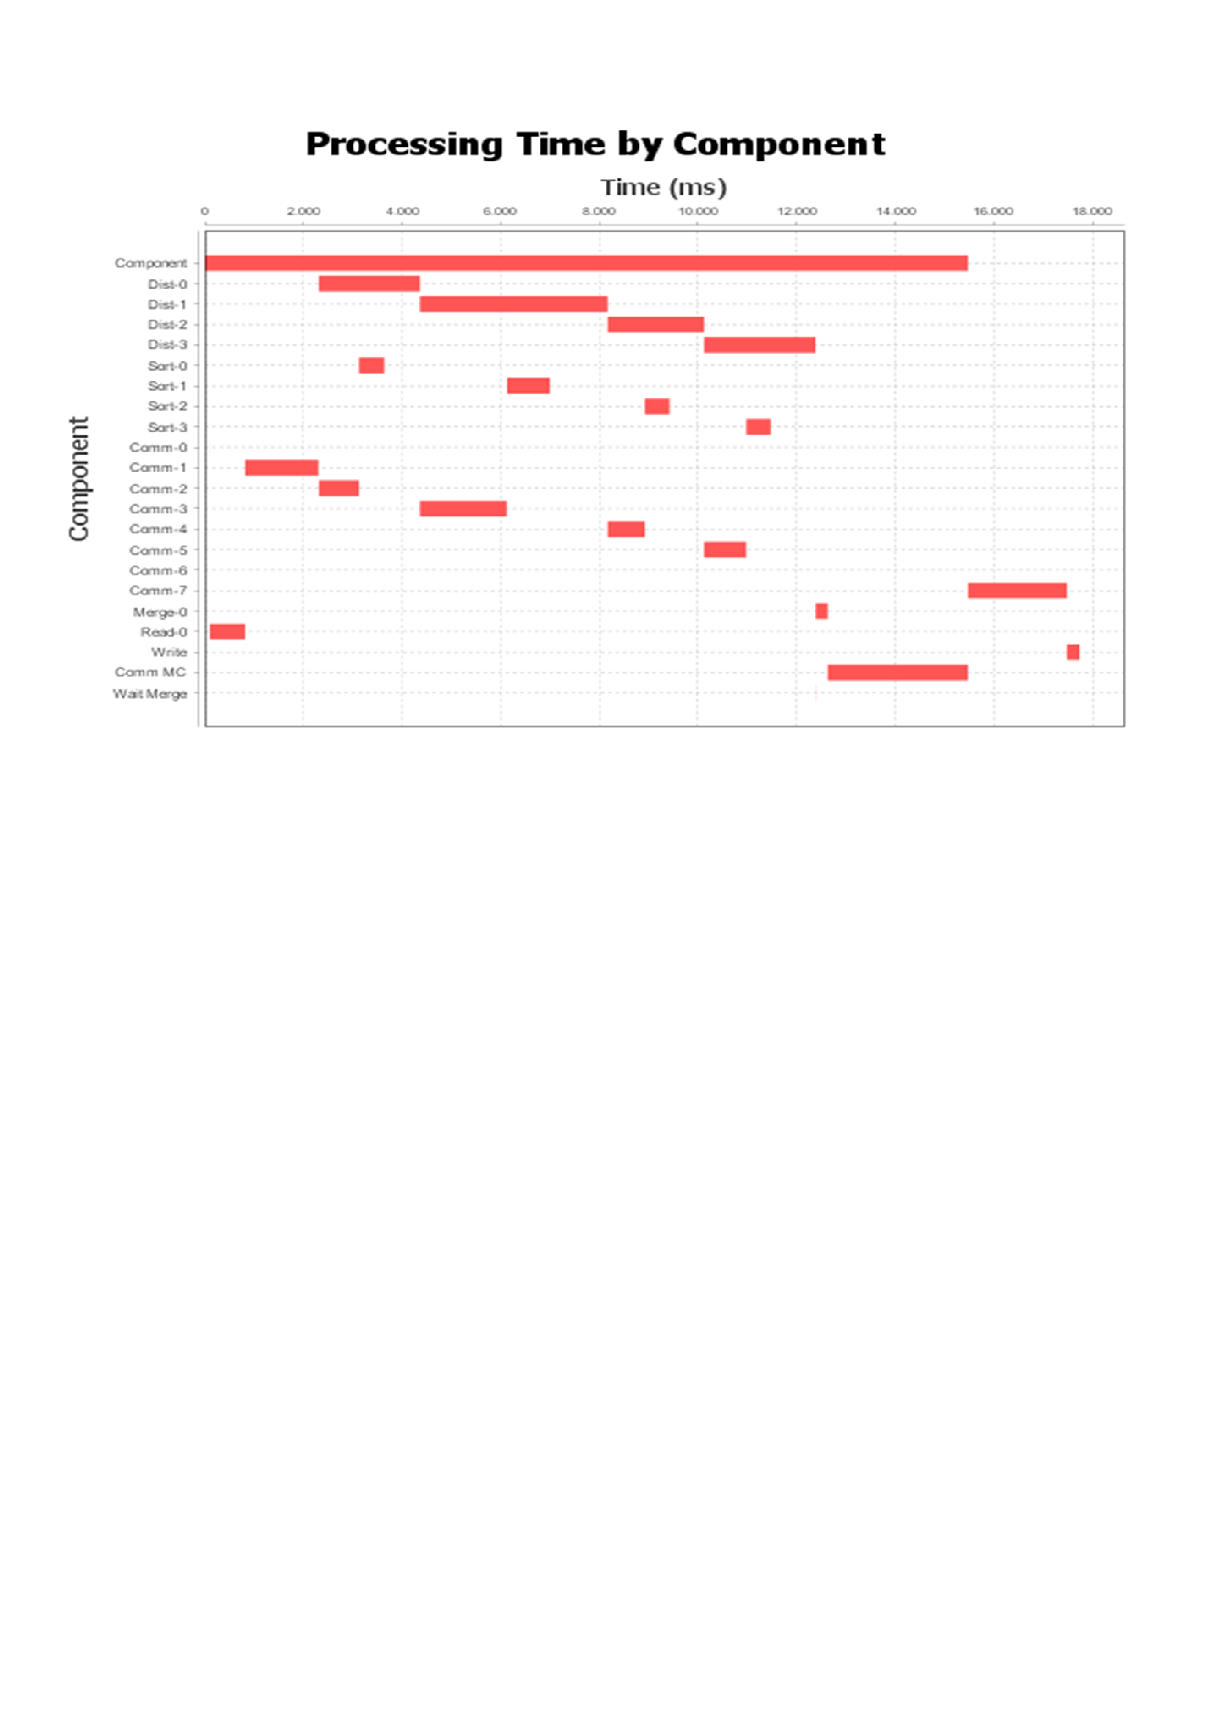
\includegraphics[trim=0.5cm 17cm -5cm 1cm, scale=0.9]{fig/LFNormaRest242Behavior.eps}
	\caption{Behavior of the Leader-Followers Design Pattern (NORMA-REST)}
	\label{fig:leaderFollowersBehaviorRest}
\end{figure}

\begin{figure}[H]
	\centering
	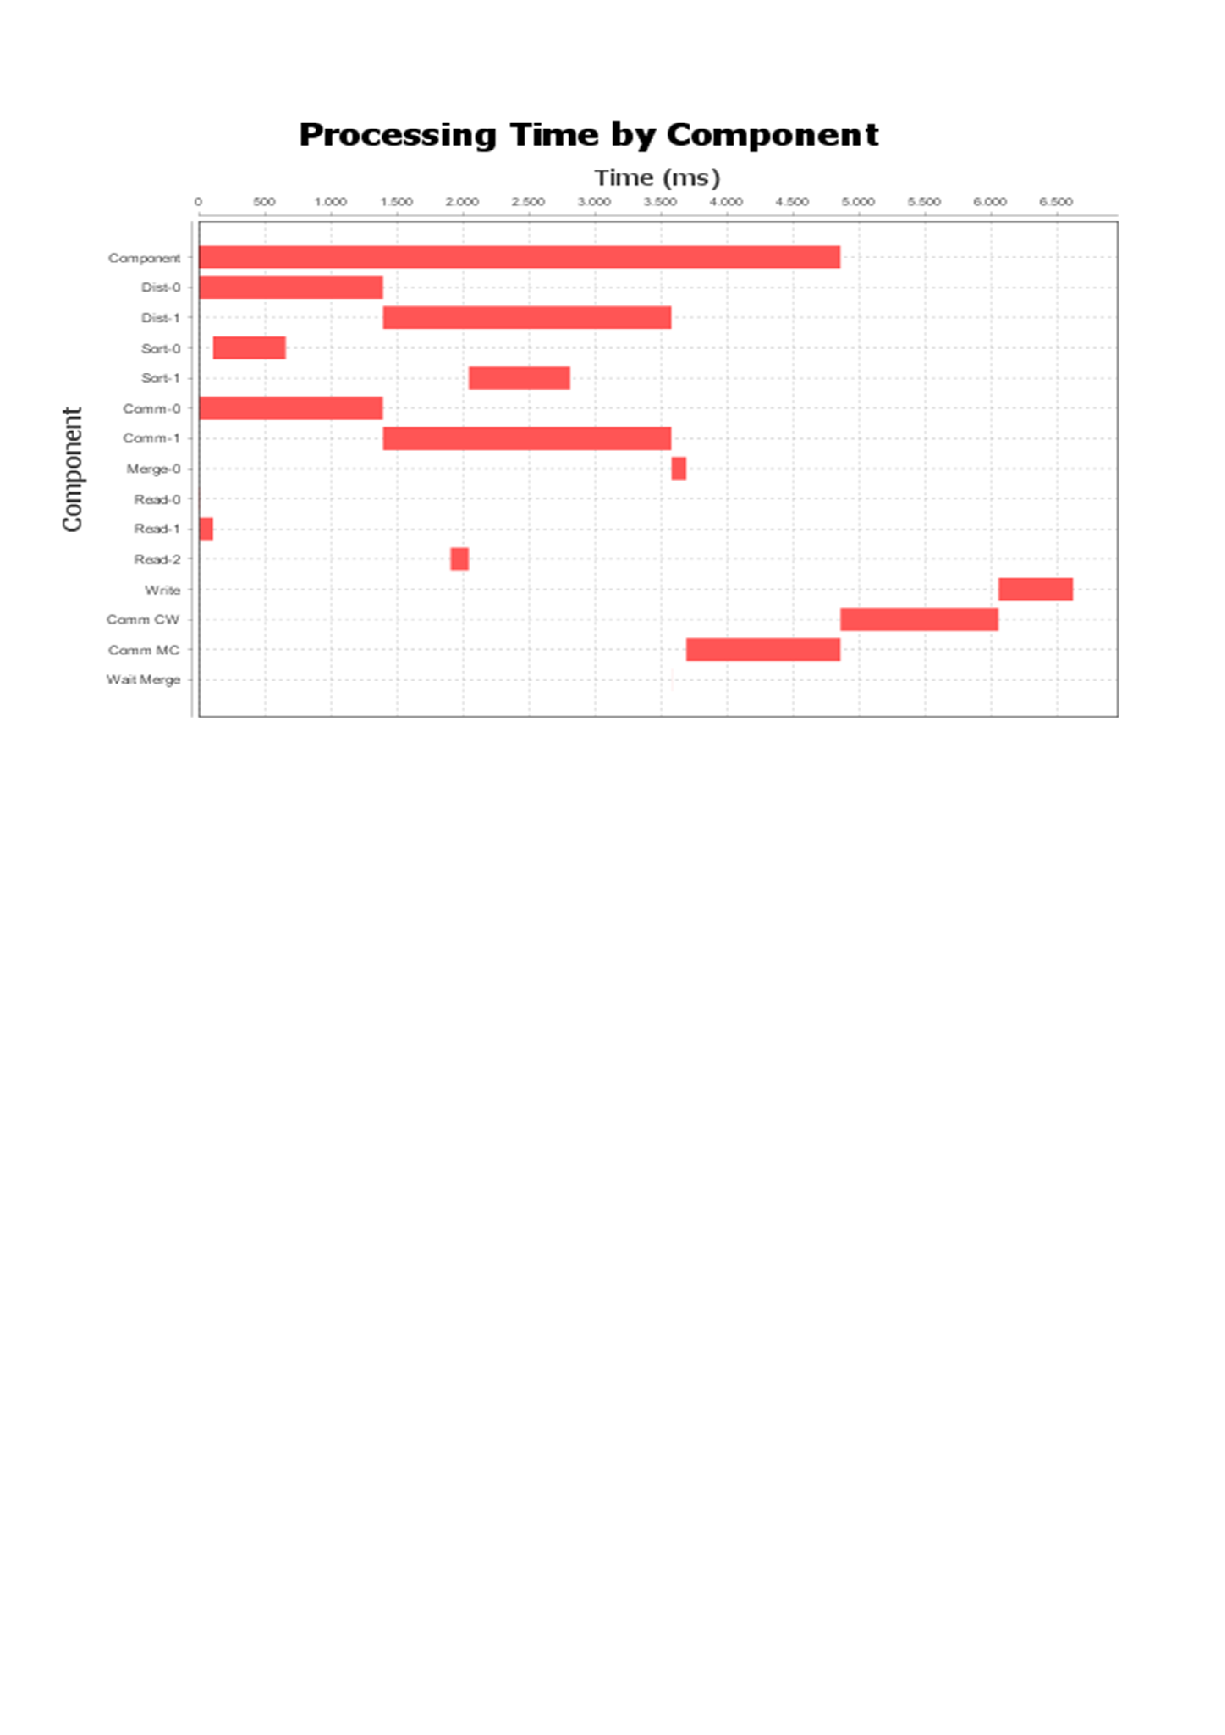
\includegraphics[trim=0.5cm 17cm -5cm 1cm, scale=0.9]{fig/LFUmaRmi422Behavior.eps}
	\caption{Behavior of the Leader-Followers Design Pattern (UMA-RMI)}
	\label{fig:leaderFollowersBehaviorRmi}
\end{figure}


\section{Latency Experiments Results}

\subsection{Consolidated Data of the Experiments Results of Controllable Variables}
\label{sebsec:consolidatedData}

Tables \ref{tab:processOriginalStrategy }, \ref{tab:processSeparationMerge}, \ref{tab:processForkJoinlibrary}, \ref{tab:processDistributedForkJoin}, and \ref{tab:processLeaderFollowers} show the experiments average processing time measured in milliseconds. For each experiments was sorted 10 files of the same size. We calculate average time for the 10 files and consolidate this information discriminating by domain-specific design pattern, communication protocol, memory structure, available nodes, and file size. Taking these tables as base we analyze each controllable variable in following sections.

According to table \ref{tab:benchmarks} we should execute 3150 experiments in the bandwidth configuration of 1GB, however, due to the thesis scope we reduce to 2561 experiments. 53,48\% of the excluded experiments correspond to the configuration of the NORMA memory structure. Due to distribution can not be leveraged in this configuration, we decide that these experiments should not be executed (see section \ref{subsec:memoryAnalysis}). 35,99\% of the excluded experiments correspond to the configuration of 16 available nodes. This decision was taken because we observe that this configuration did not improve the performance of the experiments (see section \ref{subsec:processingNodesAnalysis}).
% The 10.53\% of the excluded experiments were not executed due to previous to execute experiments of the configuration of Leader / Followers - UMA shows that this pattern had not the best results (see section \ref{}). 

The experiments of the bandwidth configuration of 100MB took too much time, therefore, taking into account the thesis scope we decide to execute just 231 experiments. These experiments were executed to verify that there is a factor of approximately 10 between the bandwidth configurations of 1GB and 100Mb. The experiments were executed in the four best configurations and four complementary configurations (see section \ref{subsec:bandwidthAnalysis}). Table \ref{tab:consolidatedData100MB} summarizes the average time of the experiments in 100MB configuration.

The missing rate of experiments was 0.078\% because only two experiments of 2561 were failed.

\begin{landscape}
	
\begin{figure}
	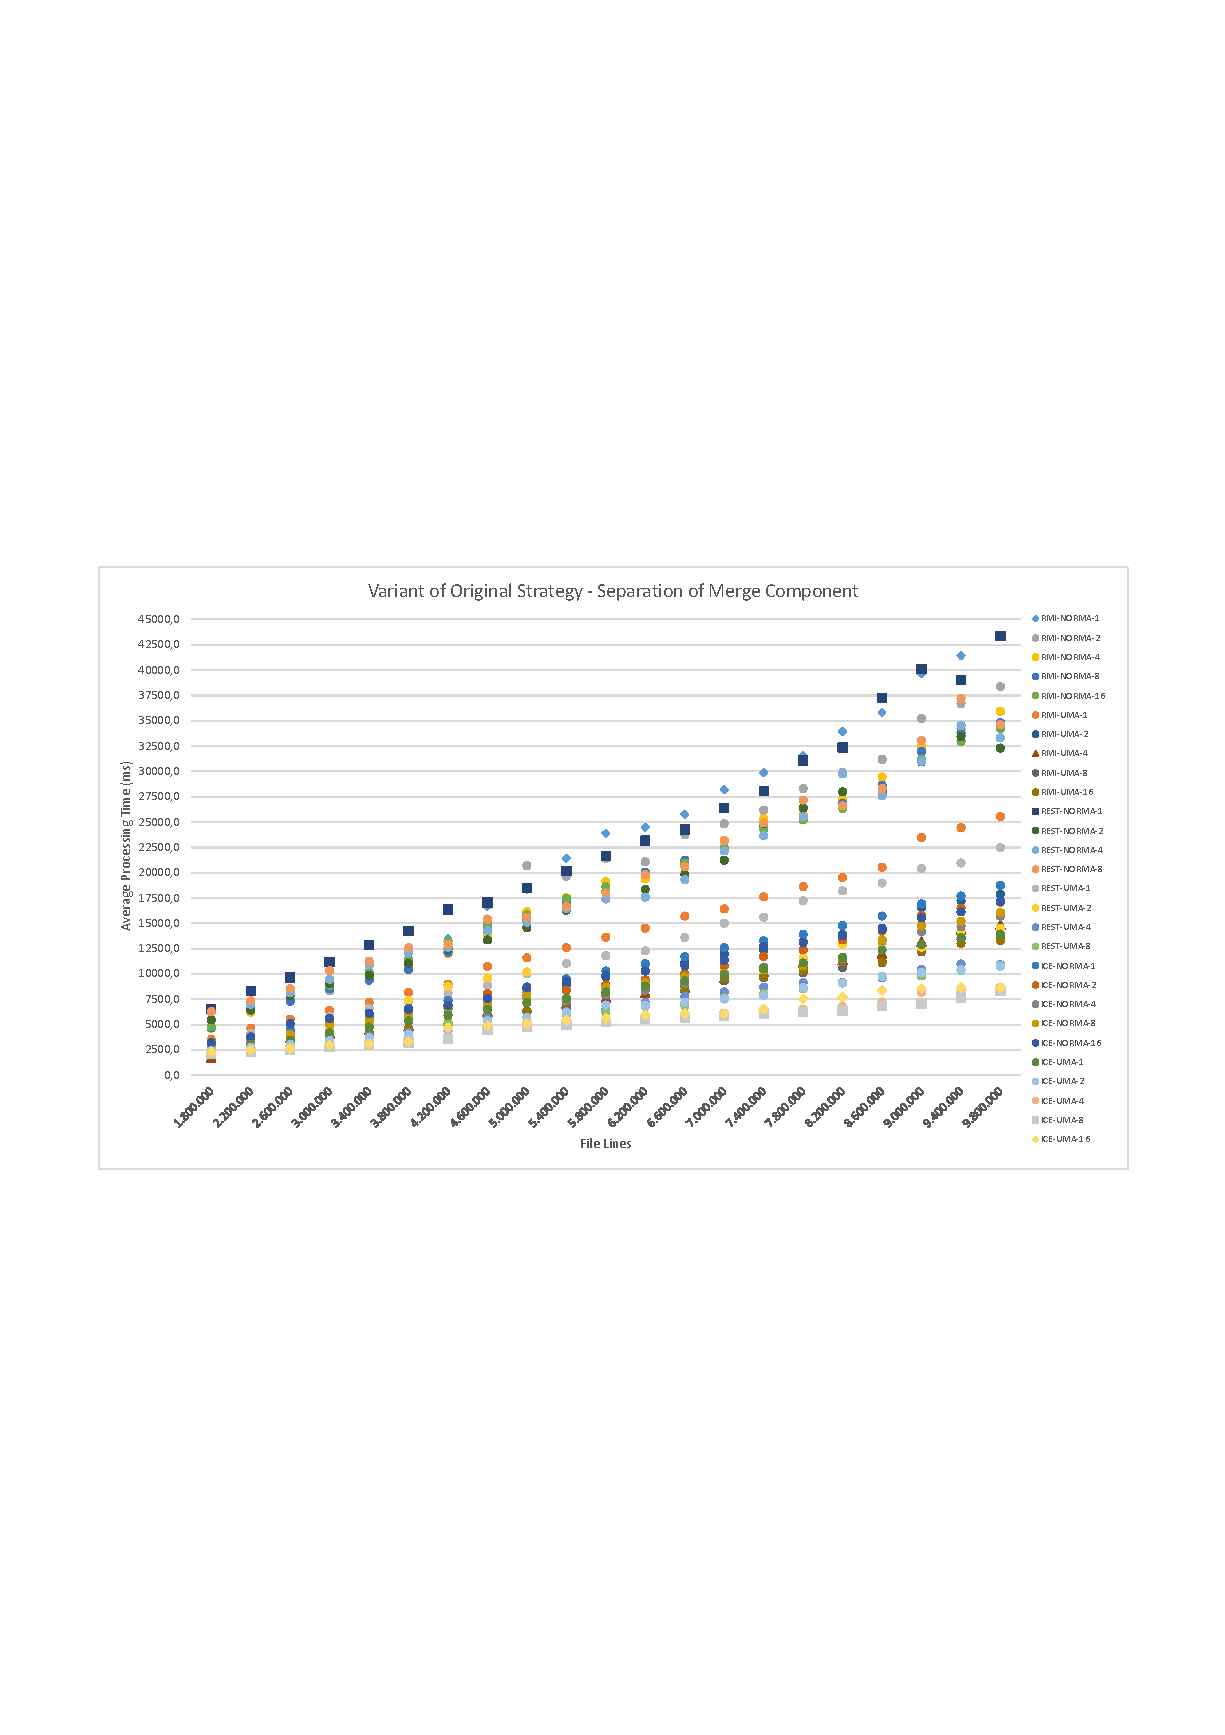
\includegraphics[trim=1cm 8cm -1cm 8cm, scale=1.3]{fig/variantOriginalStrategyGraph.eps}
	\caption{Consolidated Data of the Experiments Results of the Variant of Original Strategy - Separation of Merge Component}
	\label{fig:variantOriginalStrategyConsolidated}
\end{figure}

	% Please add the following required packages to your document preamble:
	% \usepackage{multirow}
	% \usepackage{graphicx}
	\begin{table}[]
		\centering
		\fontsize{12}{24}\selectfont
		\caption{Processing Average Time - Original Strategy - UMA}
		\label{tab:processOriginalStrategy }
		\resizebox{1.2\textwidth}{!}{%
			\begin{tabular}{|c|c|c|c|c|c|c|c|c|c|c|c|c|c|c|}
				\hline
				\multirow{3}{*}{FILE SIZE} & \multicolumn{14}{c|}{Processing Average Time - Original Strategy - UMA (ms)} \\ \cline{2-15} 
				& \multicolumn{5}{c|}{RMI} & \multicolumn{4}{c|}{REST} & \multicolumn{5}{c|}{ICE} \\ \cline{2-15} 
				& 1 & 2 & 4 & 8 & 16 & 1 & 2 & 4 & 8 & 1 & 2 & 4 & 8 & 16 \\ \hline
				1.800.000 & 2399,1 & 2390,8 & 2538,9 & 2768,1 & 2986 & 2248,2 & 2386,1 & 2424,1 & 2545 & 2228,0 & 1839,0 & 1744,5 & 1705,6 & 2162,2 \\ \hline
				2.200.000 & 3211,9 & 3111,6 & 3232,2 & 3386,1 & 3704,5 & 2889,8 & 2812,9 & 2932,2 & 3386,7 & 2597,2 & 2367,3 & 2280,5 & 2029,9 & 2576,6 \\ \hline
				2.600.000 & 3734,2 & 3633,4 & 3734,3 & 3945,7 & 4301,8 & 3330,5 & 3286 & 3328 & 3722 & 3122,0 & 2588,4 & 2639,5 & 2367,3 & 2294,5 \\ \hline
				3.000.000 & 4319,5 & 4196,8 & 4200,6 & 4449,6 & 4797,2 & 4016,6 & 3679,8 & 3833 & 4236,9 & 3662,5 & 3454,2 & 3287,1 & 3313,7 & 3433,6 \\ \hline
				3.400.000 & 4916,2 & 4693,1 & 4763,5 & 5087,5 & 5434,9 & 4607,6 & 4216,1 & 4354,4 & 4794,4 & 4179,8 & 3952,1 & 3687,2 & 3714,4 & 3785,0 \\ \hline
				3.800.000 & 5596,3 & 5235,4 & 5312,4 & 5530 & 5870,7 & 8037,1 & 6746,5 & 5060,5 & 5292 & 4677,4 & 4346,8 & 4128,1 & 4105,3 & 4163,6 \\ \hline
				4.200.000 & 5990,2 & 5827 & 5831,7 & 6190,2 & 6449,4 & 6934 & 5567,6 & 5429,2 & 5901,3 & 5217,5 & 4830,3 & 4505,2 & 4416,1 & 4639,2 \\ \hline
				4.600.000 & 7686,9 & 6770,5 & 6665,3 & 7037,9 & 7343,5 & 6113,3 & 6223,8 & 5916,1 & 6448,7 & 5730,9 & 5274,6 & 4934,1 & 4849,1 & 4938,3 \\ \hline
				5.000.000 & 8004,9 & 7281,8 & 7271 & 7669,6 & 7944,3 & 6710,9 & 6402,6 & 6434,1 & 6421,7 & 6280,7 & 5720,2 & 5304,1 & 5263,3 & 5375,5 \\ \hline
				5.400.000 & 8890,1 & 7940,3 & 7958,3 & 8309,3 & 8591,8 & 7755,8 & 7308,3 & 7191,2 & 7232,3 & 6977,3 & 6162,0 & 5697,4 & 5440,5 & 5685,6 \\ \hline
				5.800.000 & 9758,1 & 8878,3 & 8649,4 & 9172 & 9427,1 & 8622,7 & 7726,6 & 7898,2 & 6965 & 7607,6 & 6837,6 & 6206,0 & 5934,8 & 6045,2 \\ \hline
				6.200.000 & 10268 & 9415,2 & 9296,4 & 9693,5 & 10137,2 & 9661,9 & 8435,6 & 8163,1 & 8347,4 & 8179,1 & 7093,8 & 6592,0 & 6245,3 & 6197,7 \\ \hline
				6.600.000 & 11087,2 & 9987,6 & 9875 & 10266,2 & 10600,6 & 10423,4 & 9064,1 & 8878,7 & 8973,9 & 8778,6 & 7621,0 & 6886,9 & 6686,5 & 7058,9 \\ \hline
				7.000.000 & 12023,1 & 10351,9 & 10672,8 & 11019,1 & 11159,8 & 10806,4 & 9548,9 & 9226,7 & 9992,1 & 9278,3 & 8033,1 & 7415,3 & 6974,6 & 7384,9 \\ \hline
				7.400.000 & 12851,7 & 11072,8 & 11208,2 & 11503,3 & 11995,1 & 12404,6 & 11205,8 & 9267,1 & 10295,5 & 9788,1 & 8510,6 & 7754,8 & 7372,7 & 7691,9 \\ \hline
				7.800.000 & 13777,6 & 11883,2 & 11759,4 & 12225,1 & 12847,1 & 13227,4 & 11122,6 & 9552,3 & 10507,4 & 10482,5 & 9108,1 & 8194,8 & 7726,1 & 7999,4 \\ \hline
				8.200.000 & 14152,8 & 12486,2 & 12639,4 & 12559,6 & 13493,9 & 13505,8 & 12040,7 & 11528,6 & 11403,7 & 11027,1 & 9630,6 & 8512,3 & 8077,6 & 8277,1 \\ \hline
				8.600.000 & 15558 & 13274,7 & 13409,7 & 13412,5 & 14216,8 & 14527,7 & 12680,1 & 11406,7 & 11988,1 & 11795,7 & 10167,4 & 8961,1 & 8552,8 & 8662,9 \\ \hline
				9.000.000 & 16738,7 & 14754,8 & 14989 & 15359,8 & 15590,4 & 16384,7 & 14221,2 & 11399,5 & 12061,6 & 12333,4 & 10189,8 & 9305,3 & 8864,7 & 9333,5 \\ \hline
				9.400.000 & 18149,5 & 15234,6 & 15426,6 & 16167 & 16354,9 & 14441,5 & 13152,3 & 12949,6 & 12540,4 & 13182,2 & 10773,4 & 9676,8 & 9240,9 & 9595,3 \\ \hline
				9.800.000 & 19389,9 & 16185,8 & 16540,6 & 16798,6 & 17022,9 & 16812,6 & 14586,2 & 13704,6 & 14133,9 & 13692,9 & 11219,4 & 10069,0 & 9521,5 & 9998,2 \\ \hline
			\end{tabular}%
		}
	\end{table}
	
% Please add the following required packages to your document preamble:
% \usepackage{multirow}
% \usepackage{graphicx}
\begin{table}[]
	\fontsize{12}{24}\selectfont
	\centering
	\caption{Processing Average Time - Variant of Original Strategy - Separation of Merge Component}
	\label{tab:processSeparationMerge}
	\resizebox{1.45\textwidth}{!}{%
		\begin{tabular}{|c|c|c|c|c|c|c|c|c|c|c|c|c|c|c|c|c|c|c|c|c|c|c|c|c|c|c|c|c|}
			\hline
			\multirow{4}{*}{FILE SIZE} & \multicolumn{28}{c|}{Processing Average Time - Variant of Original Strategy - Separation of Merge Component  (ms)} \\ \cline{2-29} 
			& \multicolumn{10}{c|}{RMI} & \multicolumn{8}{c|}{REST} & \multicolumn{10}{c|}{ICE} \\ \cline{2-29} 
			& \multicolumn{5}{c|}{NORMA} & \multicolumn{5}{c|}{UMA} & \multicolumn{4}{c|}{NORMA} & \multicolumn{4}{c|}{UMA} & \multicolumn{5}{c|}{NORMA} & \multicolumn{5}{c|}{UMA} \\ \cline{2-29} 
			& 1 & 2 & 4 & 8 & 16 & 1 & 2 & 4 & 8 & 16 & 1 & 2 & 4 & 8 & 1 & 2 & 4 & 8 & 1 & 2 & 4 & 8 & 16 & 1 & 2 & 4 & 8 & 16 \\ \hline
			1.800.000 & 5594,7 & 4829,5 & 4653,9 & 4676,8 & 4797,7 & 3555,5 & 2809,1 & 1781,7 & 2765,9 & 2750,3 & 6573,7 & 5491,3 & 6273,3 & 6308 & 3210,7 & 2123,9 & 2776,5 & 2529,8 & 2895,9 & 3198,9 & 2905,6 & 2849,3 & 3219,6 & 2420,9 & 2464,2 & 2163,9 & 2104,1 & 2327,8 \\ \hline
			2.200.000 & 6671,9 & 6384,6 & 6225,5 & 6448,7 & 7156,2 & 4670,6 & 3398,9 & 2327 & 3174,6 & 3164,1 & 8341,1 & 6493,8 & 7026,5 & 7399,6 & 4153,9 & 3540,9 & 2946,9 & 2817,5 & 3836,9 & 3614,5 & 3304,4 & 3205,4 & 3792,9 & 3077,1 & 2770,6 & 2374,6 & 2302,6 & 2508,9 \\ \hline
			2.600.000 & 8000,7 & 7490,2 & 7368,9 & 7316,8 & 8235,1 & 5552,3 & 4507,2 & 3667,4 & 3487,8 & 3507,7 & 9648,7 & 7866,0 & 8146,2 & 8555,1 & 4985,1 & 3942,4 & 3258,9 & 3081,3 & 4524,8 & 4057,6 & 3662,5 & 4069,5 & 5128,8 & 3475,2 & 3058,1 & 2603,1 & 2521,0 & 2662,7 \\ \hline
			3.000.000 & 9180,4 & 8358,4 & 8811,1 & 8564,6 & 8902,2 & 6414,9 & 4976 & 4133,1 & 3866,6 & 3823 & 11197,3 & 9055,1 & 9484,6 & 10352,1 & 5798,1 & 4496 & 3589,4 & 3311,8 & 5324,9 & 5055,2 & 4114,5 & 5009,9 & 5638,8 & 4229,5 & 3442,3 & 2873,1 & 2777,3 & 3038,1 \\ \hline
			3.400.000 & 10349,4 & 9456,7 & 9753,1 & 9395,5 & 10148,4 & 7202 & 5485,1 & 4444,3 & 4170 & 4235 & 12858 & 9889,8 & 10928,4 & 11265,9 & 6601 & 5108,2 & 3889,8 & 3736,3 & 5982,1 & 5557,5 & 5493,7 & 5400,9 & 6134,3 & 4790,1 & 3740,0 & 3072,9 & 2976,5 & 3137,2 \\ \hline
			3.800.000 & 11586,9 & 10623,6 & 10752,6 & 10472,6 & 11346,1 & 8203,3 & 6054,6 & 4854,1 & 4564,7 & 4615,1 & 14264,3 & 11083,3 & 12132,4 & 12611,8 & 13743,7 & 7374 & 4236,2 & 5788,6 & 6642,1 & 6068,9 & 6297,6 & 6024,6 & 6487,7 & 5376,4 & 4075,9 & 3330,5 & 3256,9 & 3348,1 \\ \hline
			4.200.000 & 13480,2 & 12195,0 & 12019,1 & 12154,8 & 13226,6 & 8990,2 & 6597,5 & 5262,4 & 4923,1 & 5155,1 & 16384,2 & 12464,7 & 12640,2 & 12933,9 & 16027,1 & 8767,3 & 4648,6 & 5049,9 & 7385,5 & 6978,3 & 6838,5 & 6677,4 & 6912,1 & 5930,8 & 4399,3 & 3639,1 & 3577,2 & 4692,9 \\ \hline
			4.600.000 & 16690,0 & 15367,5 & 13878,6 & 14492,7 & 14941,0 & 10784 & 7761,3 & 6246,2 & 5689,8 & 5893,2 & 17077,1 & 13378,7 & 14305,6 & 15438,3 & 23997,8 & 9614,4 & 5656,5 & 7322,6 & 8037,2 & 8060,9 & 7582,4 & 7043,5 & 7594,1 & 6543,6 & 5373,7 & 4563,1 & 4502,9 & 4937,7 \\ \hline
			5.000.000 & 18352,9 & 20706,5 & 16159,4 & 15421,8 & 15852,1 & 11634,8 & 8318,3 & 6624,2 & 6271,8 & 6388,8 & 18504 & 14601,0 & 15132 & 15598,7 & 10033,9 & 10214 & 7923,5 & 8423,1 & 8718,5 & 8574,3 & 7672,0 & 7842,1 & 8682,7 & 7202,3 & 5718,5 & 4990,8 & 4821,3 & 5114,5 \\ \hline
			5.400.000 & 21453,5 & 19675,2 & 17559,0 & 16981,4 & 17463,8 & 12622,8 & 9010,1 & 7074,1 & 6956,4 & 7238,4 & 20191,9 & 16318,2 & 16462,4 & 16692,7 & 11059,8 & 7420,3 & 6342,5 & 6022,3 & 9524,7 & 8419,7 & 7433,4 & 7601,6 & 9253,5 & 7604,7 & 6209,9 & 5185,7 & 4998,3 & 5487,3 \\ \hline
			5.800.000 & 23901,7 & 21431,8 & 19121,0 & 18206,0 & 18623,0 & 13640,7 & 9762,7 & 7679,4 & 7946,9 & 8147,3 & 21631,8 & 17411,2 & 17416,3 & 18031,2 & 11820,1 & 8404,1 & 6477,4 & 6243,9 & 10310,0 & 8935,9 & 7971,9 & 8700,2 & 9872,2 & 8237,8 & 6944,2 & 5459,9 & 5255,7 & 5630,3 \\ \hline
			6.200.000 & 24526,2 & 21093,0 & 19404,9 & 20067,3 & 19860,4 & 14526,7 & 10356,3 & 8161,3 & 8433,1 & 8455,3 & 23165,8 & 18359,4 & 17596,4 & 19790,7 & 12291,7 & 8700,7 & 7202,4 & 6817,6 & 11022,2 & 9440,8 & 8407,6 & 9164,3 & 10303,2 & 8797,2 & 6933,2 & 5714,4 & 5608,3 & 5956,5 \\ \hline
			6.600.000 & 25791,9 & 23765,5 & 21214,1 & 21247,3 & 20939,6 & 15727,3 & 11131,1 & 8661,7 & 8821,7 & 8438,1 & 24251,2 & 19833,3 & 19338,3 & 20583 & 13618,4 & 9339,5 & 7803 & 6875,5 & 11722,6 & 10025,8 & 9107,9 & 9729,0 & 10847,1 & 9370,3 & 7222,6 & 5895,7 & 5660,8 & 6113,1 \\ \hline
			7.000.000 & 28216,4 & 24848,3 & 23227,5 & 22422,7 & 22426,9 & 16432,1 & 11971,3 & 9613,4 & 9355,8 & 9542,2 & 26389,1 & 21240,7 & 22156,7 & 23142,1 & 15018,6 & 9970,6 & 8232,3 & 7656,2 & 12606,7 & 10807,1 & 10081,5 & 10056,0 & 11378,0 & 9914,5 & 7535,1 & 6138,9 & 5855,3 & 6102,5 \\ \hline
			7.400.000 & 29904,6 & 26163,7 & 25325,9 & 24478,9 & 24289,1 & 17630,9 & 12350,8 & 10199,7 & 9643,4 & 9783,5 & 28092,2 & 24881,2 & 23676,4 & 24910 & 15618,9 & 10422,4 & 8705,4 & 8061,3 & 13294,4 & 11739,5 & 10689,3 & 10446,0 & 12750,5 & 10526,1 & 7865,8 & 6360,5 & 6071,7 & 6553,4 \\ \hline
			7.800.000 & 31582,4 & 28327,0 & 25702,6 & 25478,3 & 25232,1 & 18648,5 & 13163 & 11095,9 & 10157 & 10378,3 & 31098,9 & 26382,6 & 25523,5 & 27172,6 & 17260,4 & 11581,9 & 9166,2 & 8539,2 & 13917,8 & 12389,8 & 11107,8 & 10839,7 & 13116,9 & 11102,0 & 8648,3 & 6540,1 & 6275,5 & 7551,6 \\ \hline
			8.200.000 & 33962,8 & 29881,0 & 27190,7 & 26879,0 & 26371,8 & 19528,8 & 13902,7 & 11380 & 10626,8 & 11229,1 & 32374,6 & 27984,6 & 29757,4 & 26618,2 & 18207,1 & 12929,1 & 9188,2 & 9140,2 & 14786,4 & 13370,9 & 11532,4 & 11625,0 & 13787,3 & 11677,4 & 9118,9 & 6795,0 & 6402,3 & 7784,0 \\ \hline
			8.600.000 & 35820,9 & 31194,8 & 29462,1 & 28634,8 & 27821,8 & 20541 & 14511,4 & 11996,4 & 11123,5 & 11228,9 & 37241,5 & 28013,8 & 27629,2 & 28323,1 & 18990,1 & 12952,5 & 9613,7 & 9803,6 & 15734,5 & 14292,6 & 13304,6 & 13402,0 & 14416,8 & 12379,4 & 9791,0 & 7261,0 & 6839,2 & 8397,3 \\ \hline
			9.000.000 & 39668,1 & 35228,1 & 32479,0 & 31984,2 & 31222,6 & 23471,8 & 16579,7 & 13210 & 12192,4 & 12378,2 & 40087,8 & 30950,8 & 31038,2 & 33042,2 & 20416,6 & 12680 & 10450,4 & 9813,9 & 16933,7 & 15761,0 & 14219,5 & 14793,9 & 15548,7 & 12921,6 & 10150,9 & 8215,3 & 7117,3 & 8592,5 \\ \hline
			9.400.000 & 41421,8 & 36717,8 & 34212,1 & 33836,6 & 32973,5 & 24460,7 & 17252,2 & 14375,9 & 13448,4 & 13047,2 & 38996,2 & 33457,1 & 34531,1 & 37203,4 & 20957 & 14308,4 & 10995,1 & 10375,1 & 17701,2 & 16515,9 & 14695,9 & 15212,5 & 16152,3 & 13620,1 & 10448,9 & 8425,5 & 7691,2 & 8666,5 \\ \hline
			9.800.000 & 43339,0 & 38376,8 & 35943,9 & 34841,4 & 34235,8 & 25544,6 & 17897,5 & 14877,2 & 13562,2 & 13318 & 43393,4 & 32308,9 & 33330 & 34639,8 & 22495,2 & 14533,4 & 10948,9 & 10860,6 & 18769,5 & 17102,6 & 15725,7 & 16081,3 & 17162,6 & 13953,4 & 10785,7 & 8712,0 & 8299,0 & 8626,6 \\ \hline
		\end{tabular}%
	}
\end{table}

% Please add the following required packages to your document preamble:
% \usepackage{multirow}
% \usepackage{graphicx}
\begin{table}[]
	\fontsize{12}{24}\selectfont
	\centering
	\caption{Processing Average Time - Fork/Join Java library}
	\label{tab:processForkJoinlibrary}
	\resizebox{1.45\textwidth}{!}{%
		\begin{tabular}{|c|c|c|c|c|c|c|c|c|c|c|c|c|c|c|c|c|c|c|c|c|c|c|c|c|c|c|c|c|}
			\hline
			\multirow{4}{*}{FILE SIZE} & \multicolumn{28}{c|}{Processing Average Time - Fork/Join Java library (ms)} \\ \cline{2-29} 
			& \multicolumn{10}{c|}{RMI} & \multicolumn{8}{c|}{REST} & \multicolumn{10}{c|}{ICE} \\ \cline{2-29} 
			& \multicolumn{5}{c|}{NORMA} & \multicolumn{5}{c|}{UMA} & \multicolumn{4}{c|}{NORMA} & \multicolumn{4}{c|}{UMA} & \multicolumn{5}{c|}{NORMA} & \multicolumn{5}{c|}{UMA} \\ \cline{2-29} 
			& 1 & 2 & 4 & 8 & 16 & 1 & 2 & 4 & 8 & 16 & 1 & 2 & 4 & 8 & 1 & 2 & 4 & 8 & 1 & 2 & 4 & 8 & 16 & 1 & 2 & 4 & 8 & 16 \\ \hline
			1.800.000 & 6049,9 & 5102,4 & 4630,5 & 5478,6 & 5127,2 & 3468,1 & 3519,9 & 2550,20 & 2979,80 & 3283,7 & 5992 & 5453,0 & 5715,6 & 5798,6 & 3474,9 & 2813 & 3129,8 & 3021,1 & 3021,5 & 3409,5 & 3631,5 & 3545,8 & 3932,6 & 2132,3 & 2638,6 & 2443,4 & 2362,1 & 2518,7 \\ \hline
			2.200.000 & 6651,7 & 6127,1 & 5676,4 & 6290,0 & 6691,3 & 4454,4 & 4138,5 & 2994,90 & 3260,70 & 3711,7 & 7450,4 & 6048,2 & 6804,3 & 7208,9 & 4142,6 & 3864,8 & 3417,9 & 3287,9 & 3941,5 & 4127,8 & 3938,4 & 4400,3 & 4322,5 & 2753,6 & 2908,8 & 2627,6 & 2539,1 & 2695,1 \\ \hline
			2.600.000 & 9218,5 & 7382,0 & 7125,9 & 7117,9 & 8534,5 & 4990,7 & 4555,1 & 3694,10 & 3660,20 & 4009,2 & 8846,5 & 7178,7 & 7328 & 9483,4 & 4748,3 & 4391,9 & 3656,6 & 3531 & 4482,0 & 5003,5 & 4607,7 & 5179,6 & 4854,0 & 3104,7 & 3095,6 & 2806,6 & 2703,6 & 2860,3 \\ \hline
			3.000.000 & 9933,1 & 8066,5 & 8004,4 & 8924,6 & 9422,8 & 5673,6 & 4965 & 4159,90 & 3862,50 & 4404,7 & 9453,5 & 8269 & 8434,7 & 10064,3 & 5383 & 4684,1 & 4001,7 & 3817,1 & 5159,3 & 5042,7 & 4945,7 & 5241,4 & 5236,5 & 3374,1 & 3416,3 & 3003,4 & 2886,1 & 3059,1 \\ \hline
			3.400.000 & 11580,9 & 8913,3 & 8484,5 & 8954,7 & 10795,7 & 6425,5 & 5368,8 & 4390,40 & 4163,10 & 4774,1 & 11355,7 & 9092,3 & 9626,2 & 11527,1 & 8784,8 & 5151 & 4281,6 & 4095,7 & 5726,6 & 5432,7 & 6154,9 & 5242,8 & 6393,1 & 3988,7 & 3795,0 & 3262,9 & 3054,4 & 3488,1 \\ \hline
			3.800.000 & 12416,4 & 10955,2 & 11193,5 & 11639,2 & 12153,0 & 7051,8 & 5753,1 & 4904,70 & 4291,80 & 5146,9 & 12508,6 & 10067,1 & 10399,1 & 11877,2 & 15118 & 5658,5 & 4553 & 4606,1 & 6313,7 & 5882,1 & 6288,7 & 6064,3 & 7275,1 & 4149,0 & 4016,4 & 3481,6 & 3307,0 & 3294,2 \\ \hline
			4.200.000 & 13798,9 & 12161,1 & 12368,0 & 13089,4 & 13409,1 & 7612,3 & 5853,6 & 5038,00 & 4694,20 & 5623,6 & 13335,7 & 10980,1 & 13102,4 & 13172 & 7537,1 & 6049 & 5049 & 5174,3 & 6903,2 & 6483,3 & 6718,5 & 6746,7 & 7485,8 & 4627,0 & 4240,3 & 3657,0 & 4086,0 & 4522,3 \\ \hline
			4.600.000 & 16010,8 & 14411,3 & 14118,0 & 15397,9 & 15650,3 & 9168,8 & 6338,3 & 6021,80 & 5620,50 & 6520,8 & 14744,1 & 11618,5 & 13654,2 & 14678,6 & 8900,5 & 6747,2 & 5251,6 & 5718,9 & 7468,6 & 6795,8 & 7183,4 & 7886,6 & 7911,1 & 5797,2 & 4503,6 & 3869,0 & 4751,6 & 4671,9 \\ \hline
			5.000.000 & 17515,8 & 15807,5 & 15141,1 & 16405,6 & 16975,8 & 9775,5 & 6518,8 & 6117,60 & 6200,10 & 7609,3 & 16610,8 & 13064,8 & 14642,5 & 15828,2 & 20934,2 & 7538,4 & 5801,9 & 6165,2 & 8035,5 & 7309,2 & 7634,0 & 8434,1 & 8939,0 & 5402,0 & 4764,2 & 4044,7 & 4502,3 & 4769,5 \\ \hline
			5.400.000 & 19352,4 & 16923,3 & 16510,9 & 17262,0 & 18237,9 & 10499,5 & 7013,7 & 6335,20 & 6259,90 & 8016,8 & 17318,3 & 13953,7 & 17303,3 & 16357,3 & 9562,7 & 7104,2 & 6680,1 & 6466,3 & 8385,9 & 7517,6 & 7193,9 & 8467,3 & 9814,5 & 5667,5 & 5524,1 & 5039,3 & 4824,5 & 5038,7 \\ \hline
			5.800.000 & 20523,4 & 18406,1 & 18662,9 & 19049,1 & 19655,9 & 11485,4 & 7295,2 & 6613,40 & 7360,00 & 8853,5 & 18872,6 & 14911,7 & 18321,9 & 17350 & 10582,5 & 7931 & 7064,8 & 6746,6 & 9069,8 & 8206,3 & 7782,8 & 9450,5 & 10378,9 & 6090,5 & 5882,0 & 5283,7 & 5049,0 & 5275,3 \\ \hline
			6.200.000 & 23189,3 & 19855,9 & 19946,2 & 20779,4 & 20829,8 & 12052 & 7495,9 & 6412,60 & 7677,60 & 9354,2 & 19566 & 16860,6 & 18931,2 & 19199,2 & 10916,2 & 8193,5 & 7255 & 6913,5 & 9613,9 & 8555,4 & 8202,9 & 9862,6 & 10858,8 & 6513,9 & 6090,0 & 5459,8 & 5222,5 & 5607,5 \\ \hline
			6.600.000 & 25534,8 & 21719,2 & 21294,1 & 22079,8 & 22415,7 & 12977,5 & 8002,7 & 5635,30 & 7605,00 & 9668,5 & 23283,8 & 17217,6 & 20069,3 & 22010,4 & 11904,2 & 8907,7 & 7579,1 & 7602,3 & 10191,2 & 9045,4 & 8666,7 & 10220,2 & 11267,2 & 6811,3 & 6325,3 & 5576,4 & 5365,8 & 5728,7 \\ \hline
			7.000.000 & 27332,0 & 23607,2 & 22652,1 & 22989,0 & 23827,0 & 13519,5 & 10028,3 & 8174,30 & 8377,60 & 10262,1 & 24642,3 & 21848,7 & 23474,1 & 22339,5 & 12699,2 & 9709,7 & 8450,5 & 7832 & 10763,3 & 9424,9 & 9015,3 & 10595,2 & 11706,6 & 7129,7 & 6545,7 & 5824,8 & 5593,5 & 5737,1 \\ \hline
			7.400.000 & 29758,4 & 25350,9 & 24078,9 & 25421,3 & 25097,8 & 14376,1 & 10373 & 8315,70 & 8265,60 & 10631,9 & 25319,6 & 22263,2 & 25330,8 & 24969,8 & 13486,5 & 9796,9 & 8609,7 & 9028,4 & 11352,7 & 10034,7 & 9388,8 & 10916,9 & 12316,8 & 7688,0 & 6743,6 & 5963,6 & 5674,4 & 6270,0 \\ \hline
			7.800.000 & 31223,1 & 26415,6 & 25164,2 & 26628,6 & 26455,1 & 15880,7 & 10865,6 & 8486,80 & 8796,40 & 11443,4 & 29697 & 22370,3 & 27062,8 & 25731,4 & 14506,6 & 10751,4 & 9655,1 & 8598,2 & 11915,5 & 10961,5 & 9755,0 & 11444,1 & 13707,3 & 7831,7 & 7042,0 & 6116,1 & 5807,1 & 7083,0 \\ \hline
			8.200.000 & 32777,9 & 27983,1 & 26813,5 & 28168,9 & 27670,1 & 17232,4 & 11205,4 & 9127,30 & 8856,20 & 12368,2 & 29275,8 & 27287,9 & 29121,1 & 27956,5 & 14672,6 & 11050,1 & 9812,7 & 9564,2 & 12463,5 & 11548,6 & 10210,3 & 11950,8 & 14079,2 &  & 8039,3 & 6345,8 & 6118,1 & 7286,4 \\ \hline
			8.600.000 & 34163,9 & 29709,9 & 29137,9 & 29970,5 & 29173,2 & 16964,4 & 11851,4 & 9009,40 & 8971,40 & 12874,8 & 31133,1 & 28148,7 & 26752,6 & 28200,4 & 16972,7 & 12173,8 & 10046,7 & 10173,7 & 13290,6 & 12302,8 & 11559,6 & 13237,1 & 14809,7 & 9178,0 & 8176,5 & 6518,4 & 6283,2 & 7377,3 \\ \hline
			9.000.000 & 38597,3 & 33137,2 & 31312,0 & 32911,8 & 32750,7 & 18693,3 & 12183,9 & 10637,90 & 10214,30 & 14036,7 & 34557 & 28988,4 & 28583,6 & 30874,1 & 17218,7 & 12634 & 10325,9 & 10260,6 & 14269,1 & 13282,4 & 14085,3 & 14233,5 & 15619,5 & 9503,5 & 8414,8 & 6744,4 & 6448,3 & 7519,6 \\ \hline
			9.400.000 & 39899,7 & 34431,4 & 33882,0 & 34962,3 & 34348,5 & 19962,6 & 12634,4 & 11065,80 & 10640,60 & 14708,1 & 36153,4 & 29930,4 & 28743,2 & 32114,2 & 17372,4 & 13139,2 & 11595 & 10648,5 & 14860,7 & 13969,3 & 13261,1 & 15316,2 & 16159,6 & 10019,4 & 8587,6 & 7297,9 & 7271,0 & 7723,4 \\ \hline
			9.800.000 & 41665,8 & 36150,5 & 35500,8 & 36006,9 & 35865,7 & 21609,9 & 12796,1 & 11066,50 & 11853,10 & 15451 & 35133,4 & 29668,8 & 32250,9 & 35096,1 & 18438,3 & 13689,2 & 11502,9 & 10957,1 & 15431,5 & 14249,7 & 14494,4 & 16286,2 & 16838,8 & 10452,5 & 8981,5 & 7020,9 & 7565,6 &  \\ \hline
		\end{tabular}%
	}
\end{table}

% Please add the following required packages to your document preamble:
% \usepackage{multirow}
% \usepackage{graphicx}
\begin{table}[]
	\fontsize{12}{24}\selectfont
	\centering
	\caption{Processing Average Time - Fork/Join Java library and Distributed Fork/Join}
	\label{tab:processDistributedForkJoin}
	\resizebox{1.45\textwidth}{!}{%
	\begin{tabular}{|c|c|c|c|c|c|c|c|c|c|c|c|c|c|c|c|c|c|c|c|c|c|c|c|c|c|c|c|c|}
		\hline
		\multirow{4}{*}{FILE SIZE} & \multicolumn{28}{c|}{Processing Average Time - Fork/Join Java library and Distributed Fork/Join (ms)} \\ \cline{2-29} 
		& \multicolumn{10}{c|}{RMI} & \multicolumn{8}{c|}{REST} & \multicolumn{10}{c|}{ICE} \\ \cline{2-29} 
		& \multicolumn{5}{c|}{NORMA} & \multicolumn{5}{c|}{UMA} & \multicolumn{4}{c|}{NORMA} & \multicolumn{4}{c|}{UMA} & \multicolumn{5}{c|}{NORMA} & \multicolumn{5}{c|}{UMA} \\ \cline{2-29} 
		& 1 & 2 & 4 & 8 & 16 & 1 & 2 & 4 & 8 & 16 & 1 & 2 & 4 & 8 & 1 & 2 & 4 & 8 & 1 & 2 & 4 & 8 & 16 & 1 & 2 & 4 & 8 & 16 \\ \hline
		1.800.000 & 9009,6 & 6940 & 5689,7 & 5694,5 & 5520,9 & 7506,1 & 4428,3 & 4126,6 & 3023,9 & 3422 & 11288,1 & 8180,8 & 11784,3 & 6625,3 & 8806,7 & 5089,4 & 4442,9 & 3648,2 & 11162,7 & 7386,7 & 5144,0 & 4590,2 & 4808,1 & 10856,1 & 6880,0 & 4517,3 & 3955,4 & 3070,2 \\ \hline
		2.200.000 & 10562,9 & 8441,3 & 6698,2 & 7083,9 & 6787,6 & 8546,6 & 5124,4 & 4597,4 & 3553,7 & 3930,3 & 11819,6 & 8504 & 7383,7 & 7262,1 & 9450,8 & 5544,2 & 4821,7 & 4774 & 11871,6 & 8240,0 & 5817,0 & 5343,0 & 5340,5 & 11464,1 & 7382,4 & 4789,3 & 4232,2 & 3823,1 \\ \hline
		2.600.000 & 11847,4 & 9534,3 & 7932,1 & 7848,9 & 7892,1 & 9021,4 & 5649,9 & 4970 & 3899,4 & 4275,3 & 13250 & 9845 & 8422,3 & 8254,8 & 10363,3 & 6212 & 5225,5 & 5136 & 12518,5 & 8681,6 & 6063,5 & 5504,5 & 6000,9 & 11957,4 & 7795,1 & 5093,5 & 4397,9 & 4923,0 \\ \hline
		3.000.000 & 13563,8 & 10552,4 & 8820 & 9321 & 8920,0 & 9770,1 & 5986,6 & 5307,2 & 4396,4 & 4896,1 & 14596,9 & 10886,2 & 9219,3 & 9211,8 & 11161,1 & 6911,1 & 5623,1 & 5623,4 & 13177,8 & 9315,7 & 6937,5 & 6362,3 & 6491,1 & 12713,1 & 7803,9 & 5511,5 & 4848,7 & 5764,8 \\ \hline
		3.400.000 & 19660,2 & 13946,9 & 10785,4 & 10652 & 10947,6 & 15335,4 & 9160,3 & 7150,3 & 6048,1 & 6314,5 & 21486,6 & 15031,7 & 11405,1 & 11412,2 & 17991,3 & 10093 & 7773,5 & 6574,7 & 22451,2 & 14615,1 & 10112,5 & 7996,3 & 7273,2 & 22449,5 & 12806,2 & 8807,7 & 6461,8 & 5486,6 \\ \hline
		3.800.000 & 20955 & 15313,4 & 12277,1 & 12188,2 & 11853,4 & 16024,3 & 9719,5 & 7612,7 & 6812 & 6851,7 & 22424,8 & 16076,6 & 12665,4 & 12253,9 & 18909,1 & 10898,4 & 7788 & 7183,9 & 23114,9 & 15039,7 & 10864,1 & 8421,4 & 8091,4 & 23401,3 & 14691,0 & 9050,1 & 6717,3 & 6265,6 \\ \hline
		4.200.000 & 22300,6 & 16799,6 & 13565,5 & 13406,5 & 13064,6 & 16859,1 & 10185,5 & 8073,8 & 7305 & 7225,2 & 24051,4 & 17107,5 & 14079,2 & 13120,9 & 19545,3 & 11301,5 & 8668,2 & 7562,6 & 23850,4 & 16458,2 & 11939,7 & 9221,4 & 8395,9 & 23746,9 & 14275,5 & 9523,9 & 7342,5 & 7052,9 \\ \hline
		4.600.000 & 24666 & 18647,4 & 15312,7 & 15214,2 & 15194,3 & 18324,3 & 11213,1 & 8825,6 & 8023,3 & 8255,1 & 25365,2 & 18358,3 & 14569,2 & 14330,1 & 20300,6 & 11836,9 & 9027 & 7972,9 & 25015,0 & 17473,5 & 12854,8 & 10026,3 & 9252,9 & 25136,6 & 15176,3 & 10004,8 & 7724,1 & 6661,7 \\ \hline
		5.000.000 & 25962,7 & 20289,4 & 16857,2 & 16378,7 & 16515,4 & 19172,5 & 12298 & 9450,4 & 8855,1 & 9591,7 & 26414,6 & 19404,3 & 16292,2 & 15619 & 21043,8 & 12891,7 & 9379,5 & 9282,1 & 25556,7 & 18517,4 & 13490,9 & 11599,6 & 9699,3 & 25943,8 & 15335,1 & 10548,2 & 9861,3 & 7669,7 \\ \hline
		5.400.000 & 27389,3 & 21705,9 & 17759,1 & 17707,1 & 17945,2 & 20064,3 & 12894,8 & 10147,9 & 9382,9 & 10216,7 & 27925,8 & 20445,3 & 17042 & 16900,4 & 22299,1 & 12970,4 & 9884,9 & 8992,3 & 26367,1 & 18116,1 & 13361,0 & 11497,9 & 10326,5 & 26439,8 & 16853,5 & 11209,4 & 9792,3 & 8196,5 \\ \hline
		5.800.000 & 29267,9 & 23396,7 & 19282,6 & 19440,3 & 19321,9 & 20353,9 & 14156,2 & 10772,7 & 10012,4 & 10947,3 & 28776,4 & 21526,6 & 17951,2 & 17484,4 & 22856,9 & 13578 & 10512,3 & 9380,6 & 27244,6 & 18949,6 & 13796,4 & 12209,8 & 11785,6 & 27417,0 & 15914,9 & 11293,8 & 10228,3 & 8352,9 \\ \hline
		6.200.000 & 32406 & 25364,9 & 21696,2 & 20827,4 & 20464,4 & 21821 & 14768,8 & 11342,6 & 10420,7 & 11326,7 & 30000,8 & 22752,6 & 19993,6 & 19201,5 & 24118,5 & 14305,1 & 11063,6 & 9911,7 & 27674,2 & 20157,0 & 14001,9 & 13584,6 & 12349,4 & 28194,4 & 16131,0 & 11410,3 & 11031,9 & 8663,6 \\ \hline
		6.600.000 & 41644,8 & 31362,6 & 24063,4 & 22695,8 & 22746,2 & 35289,5 & 20986,7 & 15857,1 & 13341,5 & 13473,6 & 42407 & 30151,7 & 23994,9 & 22284,8 & 38151,8 & 21660,8 & 15606,3 & 12438,9 & 47821,9 & 32163,7 & 21601,6 & 17899,4 & 18140,7 & 49483,0 & 30358,0 & 19655,7 & 15085,8 & 14907,0 \\ \hline
		7.000.000 & 43365,4 & 32710,6 & 26305,5 & 24606,2 & 24078,3 & 35242,1 & 21787,2 & 16479,9 & 13728,7 & 14168,8 & 44450,9 & 32444,7 & 27206,1 & 25132,3 & 37743,8 & 22383,6 & 16401,5 & 13032,4 & 48807,0 & 33030,6 & 24328,5 & 19150,8 & 18748,6 & 50338,8 & 31318,8 & 21372,1 & 15055,8 & 14745,5 \\ \hline
		7.400.000 & 45314,2 & 34543,1 & 27957,6 & 26449,2 & 25252,2 & 36267,1 & 22693 & 16989,7 & 14020,2 & 14805,4 & 45266,7 & 34429,8 & 28548,2 & 27593,5 & 38576,6 & 23858,7 & 16470,4 & 14221 & 50169,2 & 34162,0 & 24778,6 & 19830,8 & 19426,8 & 51798,2 & 32052,6 & 22538,4 & 16212,2 & 15483,0 \\ \hline
		7.800.000 & 46622,8 & 36079,6 & 29191,5 & 27666,4 & 26457,1 & 37402,5 & 23491 & 17629,3 & 14775,1 & 15507,5 & 47920,3 & 35552 & 29617,3 & 26919,3 & 39678,2 & 23809,3 & 18614,1 & 13874 & 51731,7 & 35282,2 & 25747,2 & 20995,4 & 20680,5 & 52918,4 & 31780,7 & 22593,5 & 15933,9 & 16338,2 \\ \hline
		8.200.000 & 48088,2 & 37450,6 & 30653 & 29308,5 & 27977,8 & 38189,9 & 24434,9 & 18267,9 & 15057,1 & 16155,2 & 52726 & 37744,6 & 31092,8 & 28868,3 & 40667,1 & 24569,8 & 18546,1 & 14556,1 & 52646,1 & 36798,0 & 27035,7 & 22730,3 & 20886,8 & 53885,5 & 32419,0 & 22503,7 & 17419,7 & 15582,4 \\ \hline
		8.600.000 & 49609,1 & 39115,3 & 32137,9 & 30726,6 & 29692,6 & 39594,6 & 26613,2 & 19242,6 & 15649,5 & 16957,3 & 52724,3 & 39461,6 & 33077,5 & 32679,6 & 41602,1 & 25182,9 & 19244,4 & 15263,6 & 54052,6 & 38053,5 & 26890,1 & 23423,9 & 21366,5 & 55132,8 & 34018,9 & 24016,8 & 17958,1 & 16238,5 \\ \hline
		9.000.000 & 53256,9 & 42368,6 & 34918,1 & 33909,6 & 32554,1 & 41120 & 28484,6 & 20704,3 & 16944,8 & 18108,5 & 56131,8 & 42711,5 & 33575,2 & 34064,4 & 42586,7 & 25950,8 & 19843,8 & 15623,9 & 55079,0 & 39950,3 & 29641,3 & 24495,1 & 24275,9 & 55686,2 & 35009,5 & 23511,8 & 17643,2 & 16739,7 \\ \hline
		9.400.000 & 55123,4 & 44157,3 & 36510 & 35135,3 & 34251,5 & 42539,3 & 30057,6 & 22369,4 & 17957,8 & 19227 & 56178,3 & 41919,3 & 35036 & 32672 & 43349,9 & 27005,2 & 20633,9 & 16290,7 & 56099,2 & 40400,8 & 29684,9 & 25917,4 & 24498,5 & 56530,9 & 34571,8 & 24113,9 & 18994,5 & 19414,5 \\ \hline
		9.800.000 & 56531,5 & 45159,3 & 37856,1 & 37406,7 & 35537,7 & 43589,1 & 30447,1 & 22647,9 & 19649,5 & 20058,3 & 59321,8 & 43580 & 35981,6 & 36669,8 & 44296,8 & 27131 & 20957,1 & 18145,7 & 57464,7 & 42072,0 & 33211,0 & 30015,6 & 25822,9 & 57187,3 & 37188,7 & 26076,3 & 23579,3 & 19984,1 \\ \hline
	\end{tabular}%
}
\end{table}

% Please add the following required packages to your document preamble:
% \usepackage{multirow}
% \usepackage{graphicx}
\begin{table}[]
	\fontsize{12}{24}\selectfont
	\centering
	\caption{Processing Average Time - Leader-Followers}
	\label{tab:processLeaderFollowers}
	\resizebox{1.45\textwidth}{!}{%
		\begin{tabular}{|c|c|c|c|c|c|c|c|c|c|c|c|c|c|c|c|c|c|c|c|c|c|c|c|c|c|c|c|}
			\hline
			\multirow{4}{*}{FILE SIZE} & \multicolumn{27}{c|}{ (ms)} \\ \cline{2-28} 
			& \multicolumn{10}{c|}{RMI} & \multicolumn{8}{c|}{REST} & \multicolumn{9}{c|}{ICE} \\ \cline{2-28} 
			& \multicolumn{5}{c|}{NORMA} & \multicolumn{5}{c|}{UMA} & \multicolumn{4}{c|}{NORMA} & \multicolumn{4}{c|}{UMA} & \multicolumn{5}{c|}{NORMA} & \multicolumn{4}{c|}{UMA} \\ \cline{2-28} 
			& 1 & 2 & 4 & 8 & 16 & 1 & 2 & 4 & 8 & 16 & 1 & 2 & 4 & 8 & 1 & 2 & 4 & 8 & 1 & 2 & 4 & 8 & 16 & 2 & 4 & 8 & 16 \\ \hline
			1.800.000 & 5059,6 & 5099,8 & 5066,8 & 5085,9 & 6151,4 & 3308,4 & 3396,2 & 3076,7 & 3089 & 3077 & 6027 & 5672,4 & 5750,1 & 5706,5 & 3222 & 3469,4 & 3204,6 & 3216,4 & 4096,2 & 4054,8 & 3721,5 & 3774,6 & 4074,4 & 2308,6 & 2321,0 & 2312,0 & 2308,6 \\ \hline
			2.200.000 & 6548,6 & 6659,6 & 6664,1 & 6717,6 &  & 4296 & 4680,7 & 4144,9 & 4117,4 &  & 7145,1 & 7621,9 & 7394,9 & 7551,5 &  &  &  &  & 4980,1 & 5550,3 & 5229,9 & 5211,7 & 5609,5 &  &  &  &  \\ \hline
			2.600.000 & 8055,1 & 7869,1 & 7769,1 & 7853,2 & 8915,9 & 5066,1 & 5379 & 4751 & 4776,3 & 5370,4 & 8285,4 & 8309,8 & 8319,9 & 8363,9 & 4987,7 & 5534,5 & 4940,2 &  & 5808,7 & 6508,6 & 6101,9 & 6098,4 & 6469,7 & 3951,7 & 3590,9 & 3590,3 & 3599,7 \\ \hline
			3.000.000 & 9157,7 & 9157,2 & 9167,9 & 9210,3 &  & 5703,5 & 6317,3 & 5874,3 & 5483,5 &  & 10024,6 & 9860,5 & 10316,7 & 10277,5 &  & 6566,3 & 6246,4 & 5978,6 & 6972,6 & 7411,8 & 7502,9 & 7573,0 & 8042,1 & 4305,5 & 4773,2 & 4372,3 & 4351,5 \\ \hline
			3.400.000 & 10751,3 & 10732,3 & 10854,1 & 10948,9 & 11963,2 & 6907 & 7263,3 & 6964,1 & 6452,1 & 7501,7 & 10607,1 & 11345,2 & 11171,2 & 11171,3 & 6494,5 &  &  &  & 7856,5 & 8432,9 & 8445,7 & 8464,5 & 8972,7 & 4858,2 & 5412,4 & 4882,4 & 4880,1 \\ \hline
			3.800.000 & 12022,1 & 12108,1 & 12134,5 & 12169,5 &  & 7411,8 & 8114,6 & 7723,5 & 7165,5 &  & 11905,9 & 12438 & 12324,1 & 12444,4 &  & 8185,3 & 7579,4 & 7530,5 & 8633,6 & 9298,0 & 9386,0 & 9357,6 & 9921,2 & 5409,8 & 5949,3 & 5411,3 & 5444,3 \\ \hline
			4.200.000 & 13022,3 & 13118,1 & 13291,8 & 13338,0 & 14257,4 & 8227,9 & 8803,1 & 8967,3 & 7827,9 & 9587 & 13594,9 & 13921,5 & 14620,2 & 14638,7 & 8250,7 &  &  &  & 9747,9 & 10798,2 & 10764,2 & 10720,5 & 11333,4 & 6667,6 & 7089,6 &  &  \\ \hline
			4.600.000 & 15344,8 & 15728,7 & 16091,8 & 15995,5 &  & 9638,1 & 10337 & 10531,1 & 9249,6 &  & 14711,8 & 15089,1 & 15611,5 & 15960,3 &  & 10073,6 & 9888,4 & 9432,9 & 10607,9 & 11796,2 & 11713,7 & 11605,3 & 12391,7 & 7048,7 & 7754,0 & 6781,4 & 6733,8 \\ \hline
			5.000.000 & 17018,3 & 17077,8 & 17462,9 & 17663,6 & 17707,7 & 10129,3 & 10937,8 & 10677,8 & 12291,6 & 12087,1 & 15975,5 & 16339,7 & 17191,4 & 17509,1 & 9892,7 &  &  &  & 11842,9 & 12807,3 & 13252,0 & 13125,2 & 13847,6 & 8129,0 & 8146,4 & 8322,6 &  \\ \hline
			5.400.000 & 18696,6 & 18682,0 & 19085,4 & 19229,4 &  & 10882 & 11872,8 & 11568,8 & 11414,9 &  & 17309,1 & 17622,1 & 18462,9 & 18567,6 &  & 11875,9 & 11961,3 & 11964 & 12857,5 & 13760,1 & 14155,9 & 14181,9 & 14927,9 & 9068,9 & 8709,0 & 8930,0 & 8109,4 \\ \hline
			5.800.000 & 21444,6 & 21053,9 & 21452,7 & 21442,3 & 21628,8 & 12546,7 & 13652,5 & 13402,7 & 12069,9 & 12248,2 & 18229,2 & 18876,6 & 19456,2 & 20011 & 11375,5 &  &  &  & 13969,9 & 14938,5 & 15541,5 & 15214,7 & 15984,9 & 9857,8 & 9472,0 & 9651,2 & 8784,0 \\ \hline
			6.200.000 & 21670,1 & 21705,5 & 22299,7 & 22589,2 &  & 13190,3 & 14431,2 & 13633,2 & 16506,5 &  & 19712,2 & 20398,6 & 21018,4 & 21730,1 &  & 13965,7 & 13917,2 & 14197,2 & 15142,8 & 16608,5 & 17157,1 & 16808,4 & 17600,2 & 10472,7 & 10252,5 & 11194,1 & 9690,9 \\ \hline
			6.600.000 & 25294,8 & 24693,0 & 24799,3 & 25458,0 & 24700,1 & 14802,9 & 15792,8 & 15155,9 & 18124,3 & 14522,9 & 21004,1 & 21653,9 & 22356,9 & 22986 & 13195,8 &  &  &  & 16103,1 & 17593,4 & 18146,0 & 17973,4 & 18755,2 & 11096,1 & 10907,3 &  &  \\ \hline
			7.000.000 & 25712,7 & 26206,5 & 26099,5 & 26034,1 &  & 15095,3 & 16363,1 & 15953,8 & 17438,1 &  & 22241,6 & 23201,7 & 24062,3 & 24682,7 &  & 16009,1 & 16412 & 16110,2 & 17471,2 & 18841,9 & 19769,5 & 20326,4 & 18755,2 & 12193,4 & 12347,8 & 13406,2 & 10949,7 \\ \hline
			7.400.000 & 27944,4 & 27801,7 & 28315,7 & 28345,4 & 26813,6 & 16218,4 & 17435 & 16752,6 & 18378,1 & 20516,3 & 24381,7 & 24197,5 & 25727,8 & 25986,4 & 15205,2 &  &  &  & 18506,8 & 19786,1 & 20875,6 & 21597,7 & 21535,1 & 13087,7 & 12988,5 & 14135,8 & 11489,3 \\ \hline
			7.800.000 & 30387,9 & 30915,2 & 30871,4 & 31674,7 &  & 17779,8 & 19183,7 & 18614,1 & 20501,8 &  & 25249,3 & 25960,6 & 27506,6 & 27446,7 &  & 18196 & 18427,7 &  & 19365,2 & 20815,6 & 21922,4 & 22606,6 & 21535,1 & 13448,8 & 13844,4 & 15012,2 & 12262,9 \\ \hline
			8.200.000 & 31425,0 & 31134,9 & 31584,2 & 32232,7 & 29944,6 & 18238,8 & 19492,8 & 19280,1 & 21816,3 & 23569,1 & 26434,5 & 27202,8 & 28669,7 & 29166,9 & 17421,4 &  &  &  & 20925,9 & 22689,1 & 23705,8 & 24277,9 & 24426,8 & 14183,7 & 14570,1 & 16630,2 & 13313,4 \\ \hline
			8.600.000 & 32565,8 & 32703,2 & 33641,7 & 33955,9 &  & 18909 & 20687,8 & 20312,9 & 22958,8 &  & 27477,9 & 28401,7 & 31244,2 & 30084,2 &  & 20244,1 & 20810,7 & 20881,8 & 22335,4 & 24105,4 & 25084,2 & 25857,5 &  & 14850,3 & 15078,8 & 17318,4 & 13610,0 \\ \hline
			9.000.000 & 35483,4 & 35320,3 & 35530,3 & 36454,3 & 34224,5 & 20651,2 & 22189,4 & 21430 & 24018,8 & 27567 & 29111,1 & 31658,6 & 30848,6 & 31751,5 & 19342,4 &  &  &  & 23834,9 & 25714,2 & 26645,5 & 27211,4 &  & 15924,2 & 15542,7 & 17595,8 &  \\ \hline
			9.400.000 & 36977,2 & 36870,8 & 37560,4 & 38105,2 &  & 21515,4 & 22702,2 & 22510,1 & 24905,3 &  & 31968,4 & 31150,6 & 34238,1 & 32971,3 &  & 22547,2 & 22339,1 & 23476,7 & 24878,1 & 26729,4 & 27621,9 & 28441,5 &  & 16822,0 & 16199,7 & 18353,6 &  \\ \hline
			9.800.000 & 39917,2 & 40492,1 & 40766,0 & 41334,4 & 38930,9 & 23681,1 & 25182,9 & 24559,4 & 30823,4 & 24525 & 33331,8 & 33519,9 & 34391,2 & 34997,5 & 20919,9 &  &  &  & 26020,6 & 27956,6 & 28767,9 & 29531,6 &  & 17718,6 & 16792,3 & 19114,5 &  \\ \hline
		\end{tabular}%
	}
\end{table}

\end{landscape}

\subsection{File Size Analysis}
File Size variable shows a tendency to reduce its impact over processing time when this is incrementing. Table \ref{tab:percentageTimeIncrement} summarizes percentage of processing time increment due to file size increment. The Fork Join Design Pattern shows a particular behavior, it has the smallest impact caused by the file size variable, however, the file sizes 3'400.000 and 6'600.000 lines show an atypical behavior. This behavior is caused by the minimum file size to distribute. Each node divides half the input data while data size is bigger than the minimum size to distribute, 400.000 lines in this case. This division causes that there are specific file sizes where the increment is bigger than the average, for example, for all file size smaller than 800.000 lines the file would be divided half one time, but for file size bigger than 800.000 and smaller than 1'600.000 lines the file would be divided half twice. When division increasing, the file chunks increasing too, and it causes a processing time increment. In our case, we start with the file size of 1'800.000 lines, this value is bigger than 1'600.000 but smaller than 3'200.000, in this range the file would be divided three times. Therefore, we can observe that the atypical increments occur when the significant figure of the file size changes in base two, for example, 800.000, 1'600.000, 3'200.000, 6'400.000. 

% Please add the following required packages to your document preamble:
% \usepackage{graphicx}
\begin{table}[]
	\centering
	\caption{Percentage of the Processing Time Increment Due to the File Size Increment}
	\label{tab:percentageTimeIncrement}
	\resizebox{\textwidth}{!}{
			\begin{tabular}{|c|c|c|c|c|c|c|}
				\hline
				File Size & \begin{tabular}[c]{@{}c@{}}The JC Sorting Strategy\\ Average\end{tabular} & \begin{tabular}[c]{@{}c@{}}The JC Sorting Strategy\\ Variation Average\end{tabular} & \begin{tabular}[c]{@{}c@{}}Fork-Join Library\\ Average\end{tabular} & \begin{tabular}[c]{@{}c@{}}Fork-Join Design\\ Pattern Average\end{tabular} & \begin{tabular}[c]{@{}c@{}}Leader-Followers Design\\ Pattern Average\end{tabular} & Average \\ \hline
				2.200.000 & 25,2\% & 22,5\% & 17,6\% & 11,5\% & 32,2\% & 16,9\% \\ \hline
				2.600.000 & 13,4\% & 17,3\% & 15,4\% & 10,2\% & 28,1\% & 15,6\% \\ \hline
				3.000.000 & 21,0\% & 14,4\% & 9,6\% & 10,3\% & 22,6\% & 18,2\% \\ \hline
				3.400.000 & 13,3\% & 11,3\% & 12,9\% & 38,7\% & 14,8\% & 13,0\% \\ \hline
				3.800.000 & 19,2\% & 13,3\% & 12,4\% & 7,6\% & 12,5\% & 9,5\% \\ \hline
				4.200.000 & 6,3\% & 11,2\% & 8,7\% & 6,9\% & 14,3\% & 12,4\% \\ \hline
				4.600.000 & 10,7\% & 16,2\% & 12,2\% & 7,7\% & 15,4\% & 9,9\% \\ \hline
				5.000.000 & 7,3\% & 10,4\% & 11,7\% & 8,5\% & 11,5\% & 6,4\% \\ \hline
				5.400.000 & 9,7\% & 3,5\% & 4,5\% & 4,5\% & 9,8\% & 7,9\% \\ \hline
				5.800.000 & 8,4\% & 8,0\% & 8,0\% & 5,1\% & 10,0\% & 6,8\% \\ \hline
				6.200.000 & 7,3\% & 5,4\% & 5,3\% & 5,9\% & 10,0\% & 14,0\% \\ \hline
				6.600.000 & 7,3\% & 6,0\% & 5,7\% & 41,8\% & 9,1\% & 7,0\% \\ \hline
				7.000.000 & 6,1\% & 7,4\% & 8,7\% & 4,9\% & 7,9\% & 6,0\% \\ \hline
				7.400.000 & 6,6\% & 6,4\% & 5,3\% & 4,5\% & 7,2\% & 5,7\% \\ \hline
				7.800.000 & 5,2\% & 6,4\% & 5,9\% & 3,3\% & 7,6\% & 5,5\% \\ \hline
				8.200.000 & 6,1\% & 5,5\% & 5,8\% & 3,8\% & 6,0\% & 5,5\% \\ \hline
				8.600.000 & 5,7\% & 5,9\% & 5,1\% & 4,3\% & 6,7\% & 7,0\% \\ \hline
				9.000.000 & 7,2\% & 8,9\% & 7,6\% & 5,3\% & 6,3\% & 4,5\% \\ \hline
				9.400.000 & 3,3\% & 5,5\% & 4,6\% & 3,5\% & 5,4\% & 5,4\% \\ \hline
				9.800.000 & 6,7\% & 3,3\% & 4,2\% & 5,8\% & 7,3\% & 9,9\% \\ \hline
			\end{tabular}%
		}
	\end{table}
	
	The figure \ref{fig:fileSize} shows an approximation to an potential equation that describe the file size variable behavior.
	
	\begin{figure}
		\centering
		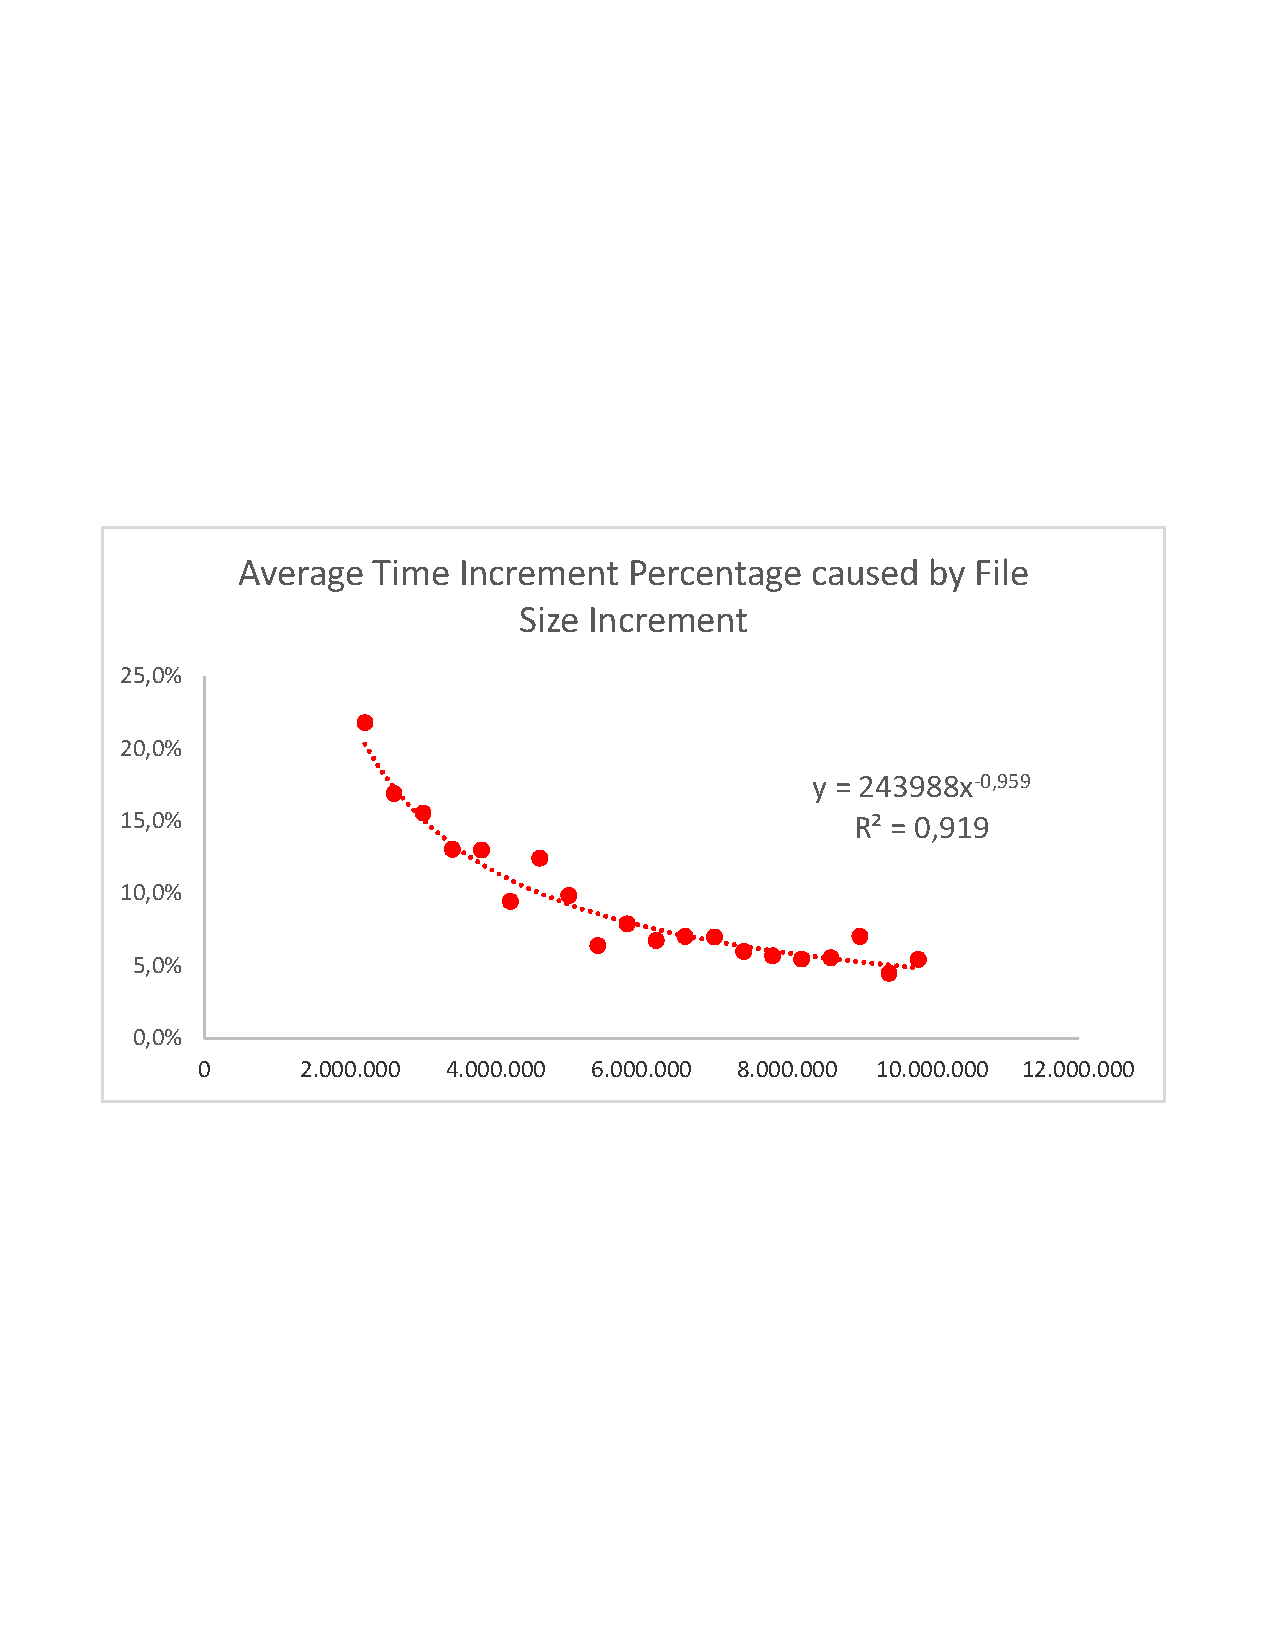
\includegraphics[trim=0cm 8.5cm -1cm 10cm, scale=0.8]{fig/fileSize.eps}
		\caption{Average Time Increment Percentage caused by File Size Increment}
		\label{fig:fileSize}
	\end{figure}

We can think that because the file size impacts each time minus the total time to process the file our proposed architectures could try to process files each time bigger. It could help us to know the limit of processing of our design patterns.

\subsection{Processing Nodes Analysis}
\label{subsec:processingNodesAnalysis}
Available processing nodes variable data was consolidated in table \ref{tab:improvementAvailableNodes}. We can observe that improvement caused by increasing the number of available nodes is not linear, that is, it does not occur that when the number available nodes are increasing the system performance is improved. By contrast, the improvement is smallest while more nodes are added. Additionally, the structure memory variable impacts the improvement achieved. Table \ref{tab:improvementAvailableNodes} shows that the Norma average improvement is smallest than the Uma memory structure. The figure \ref{fig:availableNodes} show an approximation logarithmic equation that adjusts to the behavior of the improvement percentage when the available nodes are increased.

We relate this behavior to communication time behavior. Table \ref{tab:communicationTimePercentage} summarizes the communication time percentage on the total processing time, it is worth noting that the Uma memory structure data includes the read phase time as part of the communication time, while the Norma memory structure does not. In this table is evident that the communication time percentage increases as the number available nodes increase too. 

% Please add the following required packages to your document preamble:
% \usepackage{multirow}
% \usepackage{graphicx}
\begin{table}[]
	\centering
	\caption{Average of the Improvement Percentage by Increasing Available Nodes}
	\label{tab:improvementAvailableNodes}
	\resizebox{\textwidth}{!}{%
			\begin{tabular}{|c|c|c|c|c|c|c|c|c|c|c|c|c|}
				\hline
				\multirow{2}{*}{\begin{tabular}[c]{@{}c@{}}MEMORY \\ STRUCTURE\end{tabular}} & \multirow{2}{*}{\begin{tabular}[c]{@{}c@{}}DESIGN \\ PATTERN\end{tabular}} & \multicolumn{4}{c|}{RMI (\%)} & \multicolumn{3}{c|}{REST (\%)} & \multicolumn{4}{c|}{ICE (\%)} \\ \cline{3-13} 
				&  & 2 & 4 & 8 & 16 & 2 & 4 & 8 & 2 & 4 & 8 & 16 \\ \hline
				\multirow{4}{*}{NORMA} & Original Strategy Variation & 10,23 & 6,79 & 1,35 & -2,16 & 24,74 & -2,77 & -3,95 & 8,92 & 9,64 & -1,90 & -11,24 \\ \cline{2-13} 
				& Fork/Join Java library & 16,43 & 3,00 & -5,20 & -2,58 & 20,61 & -8,26 & -4,95 & 6,49 & 1,80 & -8,74 & -8,25 \\ \cline{2-13} 
				& Fork-Join Design Pattern & 29,25 & 22,65 & 2,00 & 2,19 & 36,37 & 18,71 & 7,05 & 44,25 & 38,49 & 17,96 & 5,13 \\ \cline{2-13} 
				& Leader-Followers Design Pattern & -0,15 & -1,00 & -0,95 & -1,47 & -2,20 & -3,11 & -0,85 & -7,36 & -1,36 & -0,79 & -3,52 \\ \hline
				\multicolumn{2}{|c|}{NORMA AVERAGE} & 13,94 & 7,86 & -0,70 & -1,00 & 19,88 & 1,14 & -0,68 & 13,07 & 12,14 & 1,63 & -4,47 \\ \hline
				\multirow{5}{*}{UMA} & Original Strategy Variation & 37,58 & 26,36 & 1,71 & -1,02 & 49,82 & 30,94 & 1,53 & 24,82 & 22,62 & 4,50 & -9,69 \\ \cline{2-13} 
				& Fork/Join Java library & 39,23 & 20,98 & -1,56 & -19,02 & 44,73 & 16,21 & 2,23 & 7,37 & 15,88 & 1,19 & -7,57 \\ \cline{2-13} 
				& Fork-Join Design Pattern & 57,45 & 27,76 & 18,17 & -5,85 & 68,18 & 30,11 & 16,08 & 63,12 & 47,28 & 24,25 & 9,76 \\ \cline{2-13} 
				& Original Strategy & 10,49 & -0,91 & -4,08 & -4,55 & 10,50 & 5,74 & -4,48 & 13,99 & 8,17 & 4,32 & -4,55 \\ \cline{2-13} 
				& Leader-Followers Design Pattern & -7,00 & 4,11 & -3,52 & -2,09 & -8,51 & 2,67 & 0,48 & 9,21 & -0,92 & -3,04 & 11,15 \\ \hline
				\multicolumn{2}{|c|}{UMA AVERAGE} & 27,55 & 15,66 & 2,14 & -6,51 & 32,95 & 17,14 & 3,17 & 23,70 & 18,61 & 6,24 & -0,18 \\ \hline
				\multicolumn{2}{|c|}{AVERAGE} & 21,50 & 12,19 & 0,88 & -4,06 & 27,14 & 10,03 & 1,46 & 18,98 & 15,73 & 4,19 & -2,09 \\ \hline
			\end{tabular}%
		}
	\end{table}
	
	\begin{figure}
		\centering
		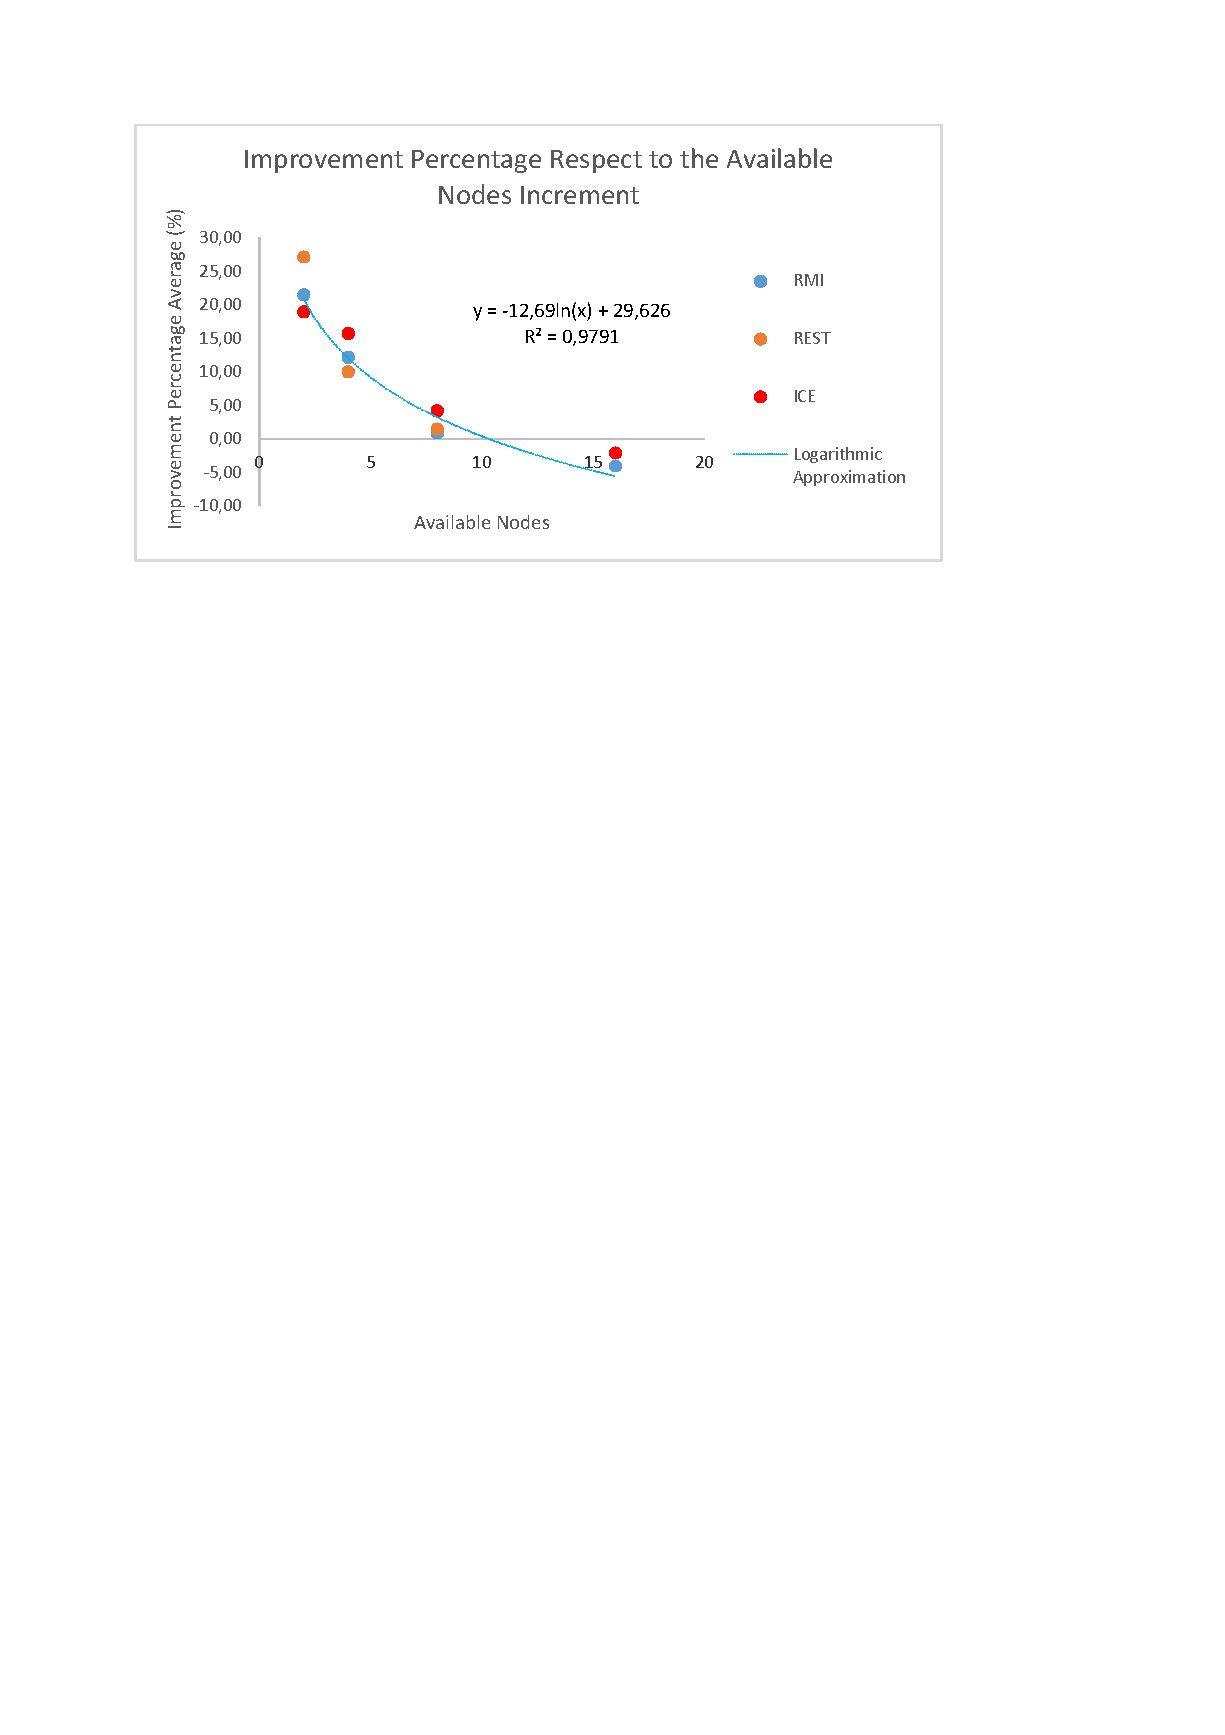
\includegraphics[trim=0.5cm 19cm 1cm 1cm]{fig/availableNodes.eps}
		\caption{Improvement Percentage Respect to the Available Nodes Increment}
		\label{fig:availableNodes}
	\end{figure}

\subsection{Communication Protocol Analysis}
According to the chart \ref{fig:betterTimesCommunicationProtocol} Ice is the best communication protocol among the studied protocols. The protocols Rest and RMI were implemented over the FraSCAti middleware and this middleware could be a factor that influence this result. 

Currently, Rest is a very used protocol due to it allows us to inter-operate among different software systems, but, if you are searching for more performance for your application you should evaluate to use another alternative such as Ice. \\
%Make Graphics comparisonCommunicationProtocols.eps betterTimesCommunicationProtocol.eps

If we compare the performance of communication protocols in pairs such as in the chart \ref{fig:comparisonCommunicationProtocols}, we can observe that if we only compare Rest vs Rmi, Rest has a better performance in 60\% times. This says to us that although Rmi in the whole experiment has a bigger amount of test with more performance (10,34\%), Rest could have better performance than RMI if we have only these two options.
\begin{figure}[H]
	\centering
	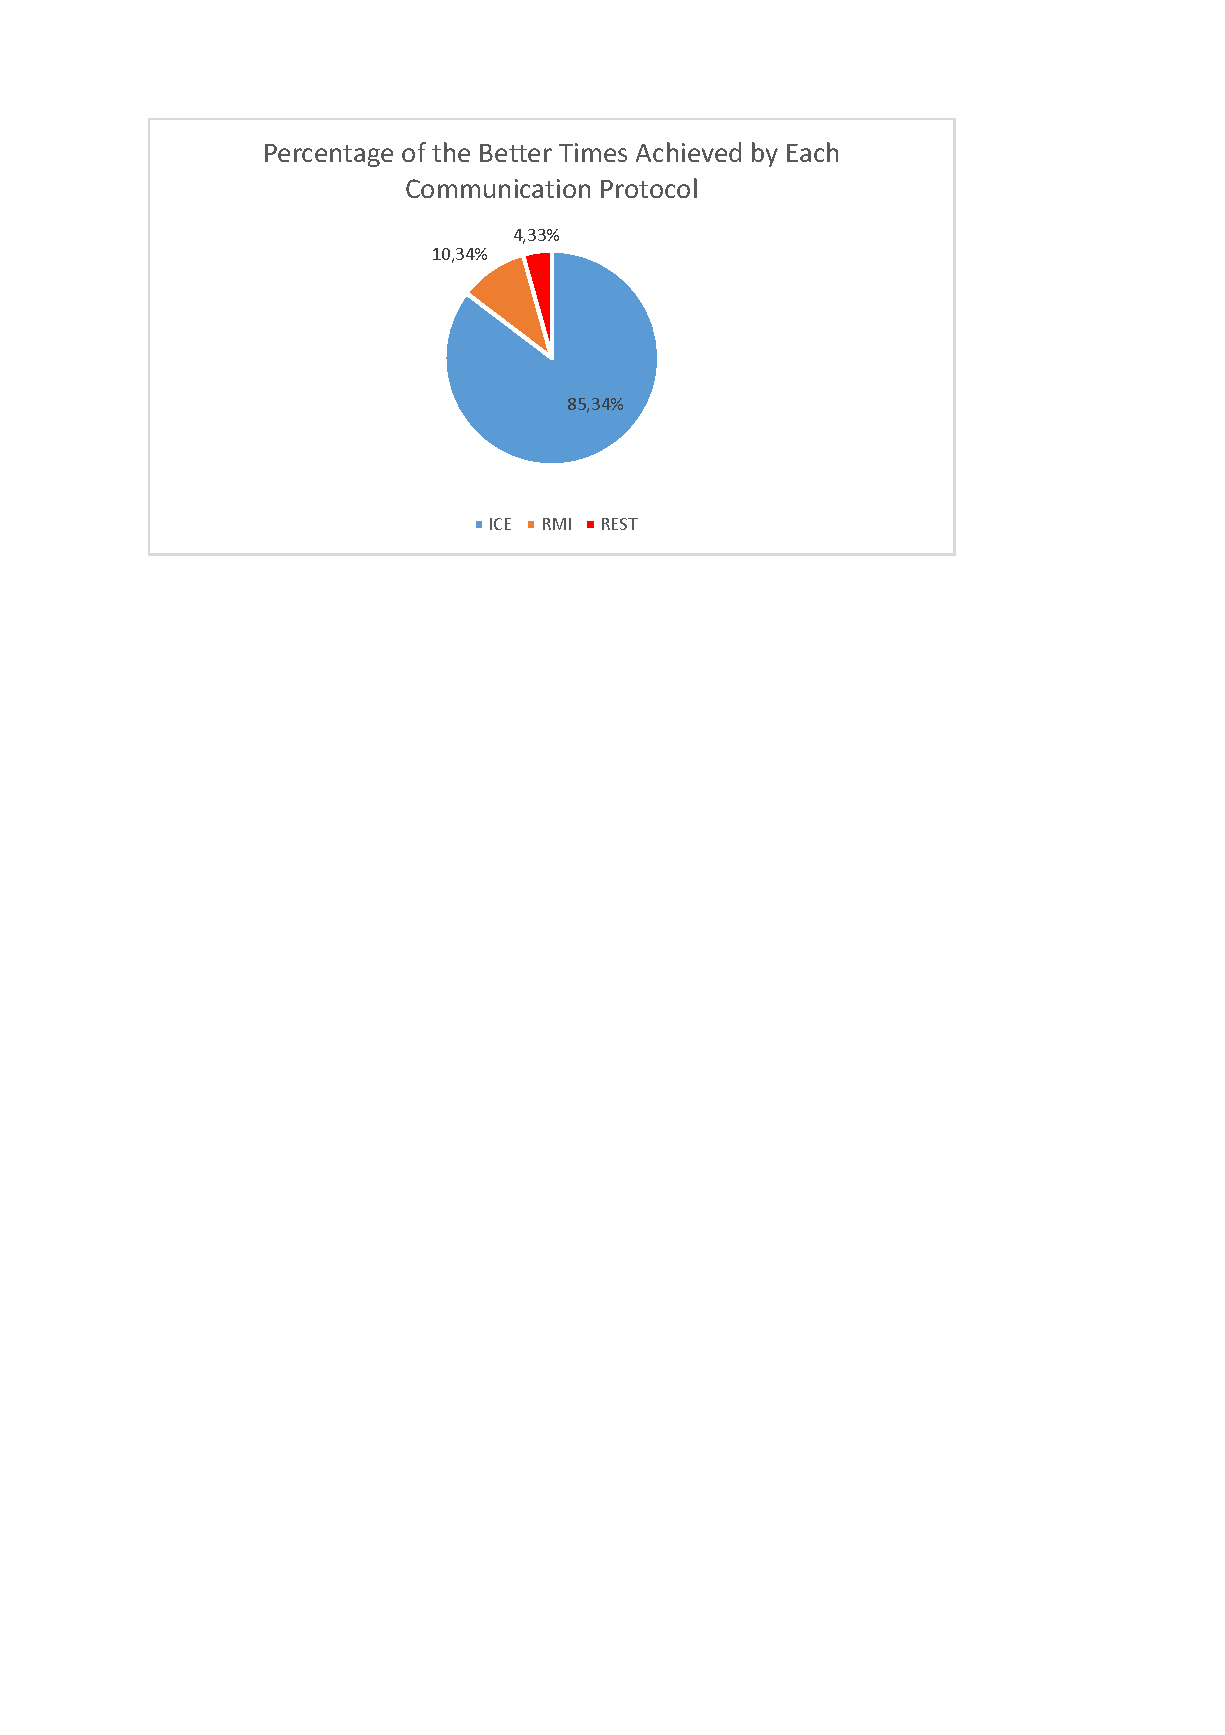
\includegraphics[trim=0.5cm 19cm 1cm 1cm]{fig/betterTimesCommunicationProtocol.eps}
	\caption{Percentage of the Better Times Achieved by Each Communication Protocol}
	\label{fig:betterTimesCommunicationProtocol}
\end{figure}

\begin{figure}[H]
	\centering
	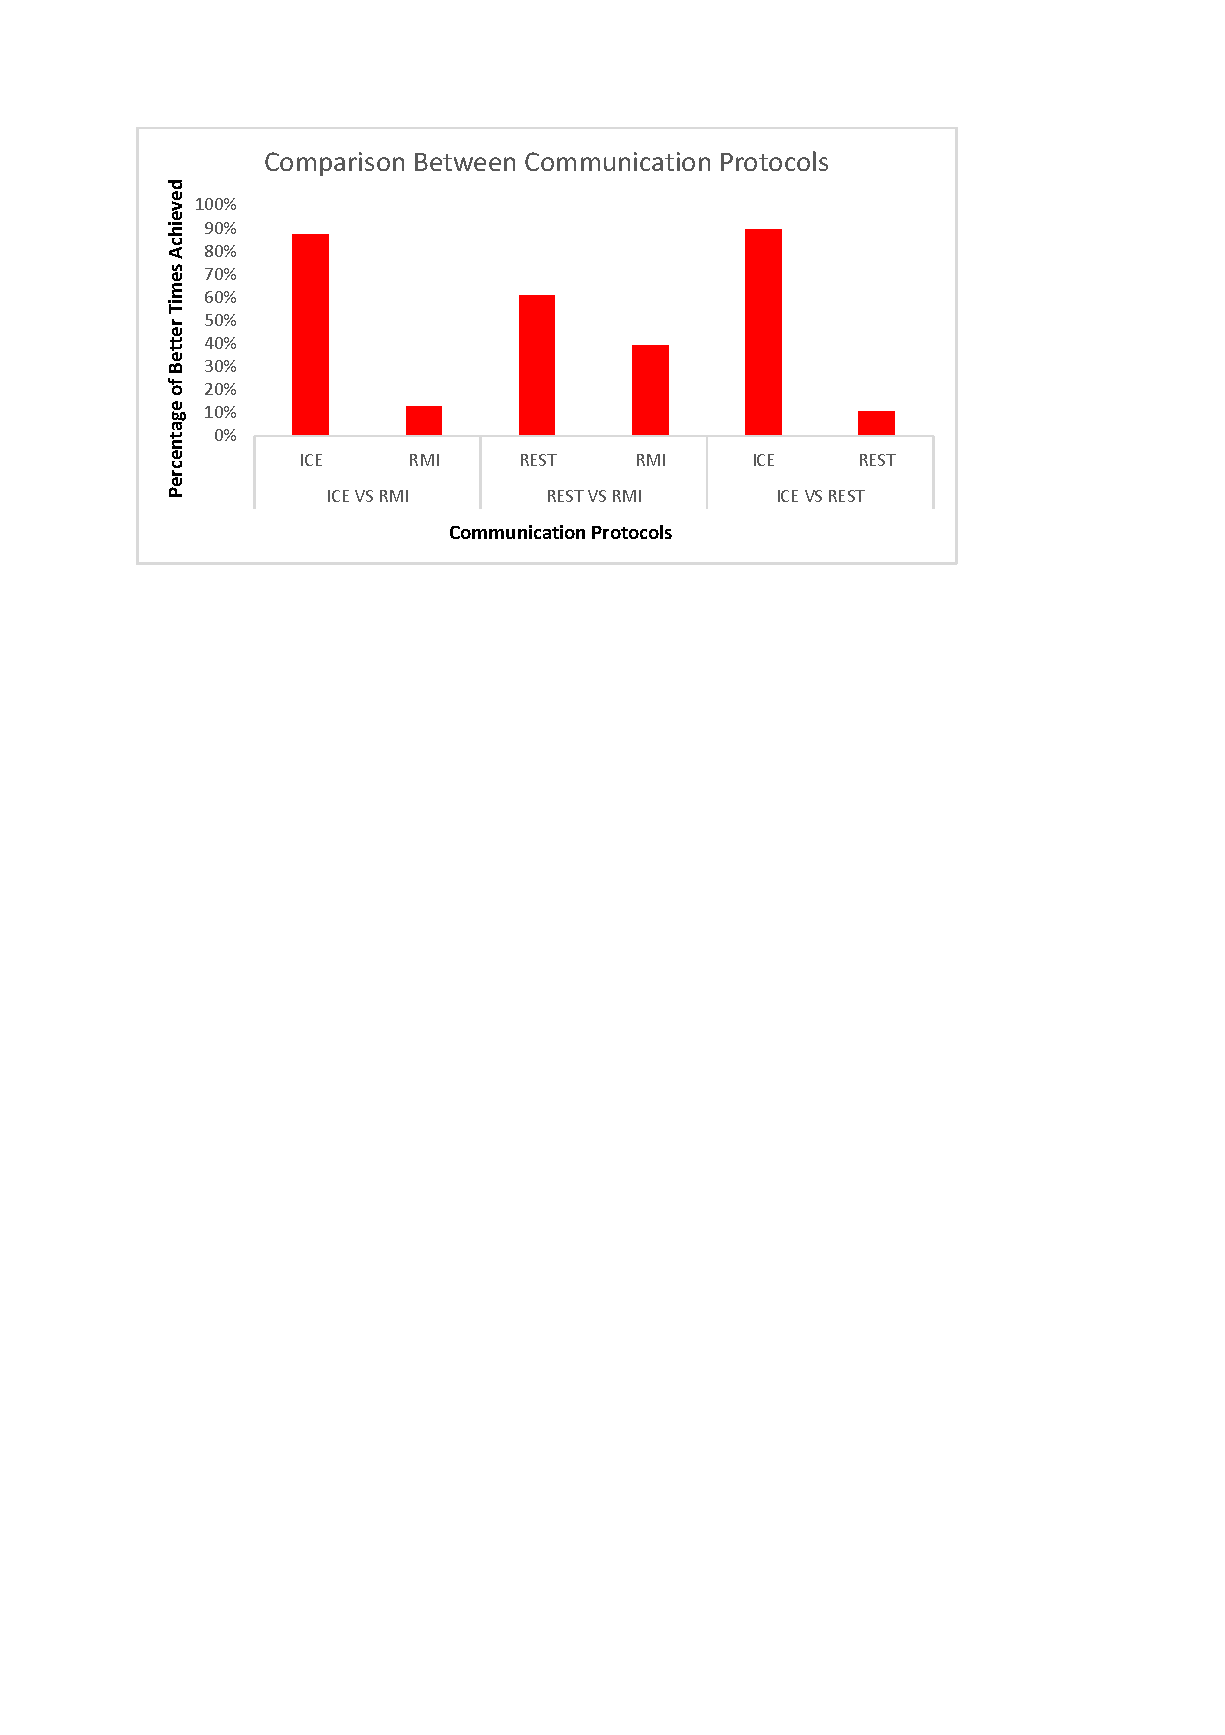
\includegraphics[trim=0.5cm 19cm 1cm 1cm]{fig/comparisonCommunicationProtocols.eps}
	\caption{Comparison Between Communication Protocols}
	\label{fig:comparisonCommunicationProtocols}
\end{figure}

\subsection{Memory Structure Analysis}
\label{subsec:memoryAnalysis}

When we start the memory analysis the first conclusion that is evident is that UMA is the best memory configuration if we are searching for the best performance. UMA has pros y cons at the same that NORMA, but the more important consideration is the bottleneck that this configuration could have. Table \ref{tab:memoryAverage} shows the percentage of times that UMA was better than NORMA. When Ice is the communication protocol UMA always is better than NORMA in more than 60\% of cases.  

% Please add the following required packages to your document preamble:
% \usepackage{multirow}
% \usepackage{graphicx}
\begin{table}[H]
	\centering
	\caption{Average of the Total Time Percentage of the Uma Memory Structure Respect to the Norma Memory Structure.}
	\label{tab:memoryAverage}
%	\resizebox{\textwidth}{!}{%
		\begin{tabular}{|c|c|c|}
			\hline
			\begin{tabular}[c]{@{}c@{}}Communication\\  Protocol\end{tabular} & \begin{tabular}[c]{@{}c@{}}Design\\  Pattern\end{tabular} & Average \\ \hline
			\multirow{4}{*}{RMI} & \begin{tabular}[c]{@{}c@{}}Original Strategy \\ Variation\end{tabular} & 47,9\% \\ \cline{2-3} 
			& \begin{tabular}[c]{@{}c@{}}Fork/Join\\ Java library\end{tabular} & 44,6\% \\ \cline{2-3} 
			& \begin{tabular}[c]{@{}c@{}}Fork-Join\\  Design Pattern\end{tabular} & 62,2\% \\ \cline{2-3} 
			& \begin{tabular}[c]{@{}c@{}}Leader-Followers \\ Design Pattern\end{tabular} & 63,4\% \\ \hline
			\multirow{4}{*}{REST} & \begin{tabular}[c]{@{}c@{}}Original Strategy\\  Variation\end{tabular} & 44,4\% \\ \cline{2-3} 
			& \begin{tabular}[c]{@{}c@{}}Fork/Join\\ Java library\end{tabular} & 45,6\% \\ \cline{2-3} 
			& \begin{tabular}[c]{@{}c@{}}Fork-Join\\  Design Pattern\end{tabular} & 64,9\% \\ \cline{2-3} 
			& \begin{tabular}[c]{@{}c@{}}Leader-Followers\\  Design Pattern\end{tabular} & 64,1\% \\ \hline
			\multirow{4}{*}{ICE} & \begin{tabular}[c]{@{}c@{}}Original Strategy\\  Variation\end{tabular} & 65,4\% \\ \cline{2-3} 
			& \begin{tabular}[c]{@{}c@{}}Fork/Join\\ Java library\end{tabular} & 60,6\% \\ \cline{2-3} 
			& \begin{tabular}[c]{@{}c@{}}Fork-Join \\ Design Pattern\end{tabular} & 85,9\% \\ \cline{2-3} 
			& \begin{tabular}[c]{@{}c@{}}Leader-Followers\\  Design Pattern\end{tabular} & 60,7\% \\ \hline
		\end{tabular}%
%	}
\end{table}

In Rest and RMI, UMA is better than NORMA in more than 60\% of cases only for the Fork-Join and Leader/Followers design patterns and in more than 40\% of times for the Original Strategy Variation and the Fork-Join Java Library. It looks like the last strategies could generate a bottleneck before the other strategies. This behaviour could be justified due to the Fork-Join and the Leader-Followers design patterns send the tasks to their processing units and these can process from that moment (i.e. a structure more horizontal), but another design patterns use a structure more hierarchical.


Due to the consistent behavior observed in this variable, we try to generate a statistical model that can predict its behavior. We try a linear regression and the ANOVA, in the tables \ref {tab:regressionStatistics} and \ref {tab:regressionStatisticsData} we summarize the results obtained. First, we can see that based on the coefficient of determination (R2) and the adjusted coefficient of determination (adjusted R2) this model is not the best to represent the behavior of memory structure. These coefficients of determination are indicators between the range 1-0, the closer to 1 the better the model, and we have 0,425 and 0,423 respectively. Second, we have multifactorial ANOVA. This model considers the effect of each studied variable and according to the P-value indicator, this is a good model to predict the structure memory variable. The P-value is used to validate the hypothesis proposed, the proposed hypothesis says that for each variable, it is significant to construct the model of the memory structure. If the calculated P-value of the variable is less than 0,05 so, the variable is accepted for the model.

\begin{table}[H]
	\centering
	\caption{Regression Statistics}
	\label{tab:regressionStatistics}
	\begin{tabular}{|l|l|}
		\hline
		Multiple R & 0,652070218 \\ \hline
		R Square & 0,425195569 \\ \hline
		Adjusted R Square & 0,423060733 \\ \hline
		Standard Error & 0,111858357 \\ \hline
		Observations & 1082 \\ \hline
	\end{tabular}
\end{table}

\begin{table}[H]
	\centering
	\caption{Regression Statistics Data}
	\label{tab:regressionStatisticsData}
	\resizebox{\textwidth}{!} & \textit{Upper 95\%} & \textit{Lower 95,0\%} & \textit{Upper 95,0\%} \\ \hline
			Intercept & 0,384230933 & 0,014801709 & 25,95855285 & 8,9435E-116 & 0,355187478 & 0,413274387 & 0,355187478 & 0,413274387 \\ \hline
			\begin{tabular}[c]{@{}c@{}}File \\ Size\end{tabular} & -6,91906E-09 & 1,40333E-09 & -4,930466112 & 9,49415E-07 & -9,67262E-09 & -4,16549E-09 & -9,67262E-09 & -4,16549E-09 \\ \hline
			\begin{tabular}[c]{@{}c@{}}Available \\ Nodes\end{tabular} & -0,007141392 & 0,000706497 & -10,10816596 & 5,19951E-23 & -0,008527659 & -0,005755125 & -0,008527659 & -0,005755125 \\ \hline
			\begin{tabular}[c]{@{}c@{}}Design \\ Pattern\end{tabular} & 0,05680204 & 0,00317531 & 17,88865847 & 7,30488E-63 & 0,050571544 & 0,063032535 & 0,050571544 & 0,063032535 \\ \hline
			\begin{tabular}[c]{@{}c@{}}Communication \\ Protocol\end{tabular} & 0,076994391 & 0,003991936 & 19,28748296 & 1,95675E-71 & 0,069161538 & 0,084827244 & 0,069161538 & 0,084827244 \\ \hline
		\end{tabular}%
	}
\end{table}

Thus, the formula that predicts the memory structure behavior is showed in the equation \ref{eq:memory}.

\begin{equation}
\label{eq:memory}
\resizebox{.92\hsize}{!}{$Uma Respect Norma = 0,384230933 - 6,91905547282634E^{-09}(fs) - 0,00714139220840687(n) + 0,0568020397510634(dp) + 0,0769943910761448(cp)$}
\end{equation} 

\subsection{Bandwidth Analysis}
\label{subsec:bandwidthAnalysis}
% Please add the following required packages to your document preamble:
% \usepackage{multirow}
% \usepackage{graphicx}

The bandwidth variable was tested using two values, 100MB and 1GB. Table \ref{tab:consolidatedData100MB} summarizes the times that each one of these tests takes with a configuration of 100MB. When we compare these tests with the same configuration executed at 1GB (reference section \ref{sebsec:consolidatedData}) we can verify that the relation between them is approximately 10 times. Table \ref{tab:calculatedRelation} summarizes this information. 

\begin{table}[H]
	\label{tab:consolidatedData100MB}
	\fontsize{16}{36}\selectfont
	\centering
	\begin{center}
		\caption{Consolidated Data of the Experiments with Bandwidth Configuration of 100MB}
	\end{center}
	\resizebox{\textwidth}{!}{%
		\begin{tabular}{|c|c|c|c|c|c|c|c|c|c|c|c|c|c|c|c|c|c|c|c|c|c|}
			\hline
			\multirow{4}{*}{File Size} & \multicolumn{13}{c|}{ICE} & \multicolumn{2}{c|}{RMI} & \multicolumn{6}{c|}{REST} \\ \cline{2-22} 
			& \multicolumn{7}{c|}{Fork/Join Java library (ms)} & \multicolumn{3}{c|}{\begin{tabular}[c]{@{}c@{}}Variant of Original \\ Strategy - Separation\\ of Merge Component\\  (ms)\end{tabular}} & \multicolumn{3}{c|}{\begin{tabular}[c]{@{}c@{}}Original\\  Strategy \\ (ms)\end{tabular}} & \begin{tabular}[c]{@{}c@{}}Original\\ Strategy\\ (ms)\end{tabular} & \begin{tabular}[c]{@{}c@{}}Fork/Join\\ Java\\ library\\ (ms)\end{tabular} & \multicolumn{3}{c|}{\begin{tabular}[c]{@{}c@{}}Original \\ Strategy \\ (ms)\end{tabular}} & \multicolumn{3}{c|}{\begin{tabular}[c]{@{}c@{}}Fork/Join \\ Java library \\ (ms)\end{tabular}} \\ \cline{2-22} 
			& \multicolumn{4}{c|}{UMA} & \multicolumn{3}{c|}{NORMA} & \multicolumn{3}{c|}{UMA} & \multicolumn{3}{c|}{UMA} & UMA & NORMA & \multicolumn{3}{c|}{UMA} & \multicolumn{3}{c|}{NORMA} \\ \cline{2-22} 
			& 2 & 4 & 8 & 16 & 2 & 4 & 8 & 2 & 4 & 8 & 2 & 4 & 8 & 2 & 2 & 2 & 4 & 8 & 2 & 4 & 8 \\ \hline
			1.800.000 & 16970,1 & 15747,4 & 16733,7 & 17388,7 & 29793,3 & 36149,5 & 40443,3 & 15896,7 & 18999,8 & 17262,9 & 17571,4 & 20704,5 & 21963,4 & 22247,5 & 36675,2 & 33466,7 & 36550,0 & 40886,3 & 55660,1 & 70549,5 & 76135,3 \\ \hline
			2.600.000 & 26006,9 & 22744,6 & 22814,6 & 24181,8 & 45621,2 & 53643,7 & 55298,5 & 26367,1 & 26774,8 & 24957,6 & 25699,9 & 29028,6 & 32459,2 & 27127,4 & 53819,9 & 41573,8 & 54247,3 & 56516,4 & 85747,8 & 100979,9 & 111670,8 \\ \hline
			3.400.000 & 31183,4 & 29276,5 & 32671,9 & 31612,3 & 59213,8 & 67254,1 & 77418,1 & 29368,9 & 34714,3 & 32498,1 & 30343,7 & 38117,7 & 41593,0 & 39617,0 & 69648,2 & 61099,4 & 72217,7 & 76444,5 & 108606,5 & 136715,9 & 145883,6 \\ \hline
			4.200.000 & 38727,3 & 35737,9 & 39156,8 & 38823,6 & 72797,2 & 83911,4 & 89244,4 & 43189,2 & 42182,2 & 38737,6 & 35171,0 & 49083,4 & 51904,5 & 43854,5 & 85884,3 & 78947,9 & 83770,1 & 94894,8 & 137490,8 & 167252,0 & 171630,6 \\ \hline
			5.000.000 & 49180,3 & 42478,2 & 44179,1 & 45303,9 & 88363,8 & 97659,8 & 107022,1 & 46358,1 & 50815,6 & 48795,8 & 47591,4 & 59010,7 & 62616,9 & 58106,6 & 102930,3 & 89540,4 & 106118,6 & 107609,2 & 164964,1 & 196633,3 & 208206,1 \\ \hline
			5.800.000 & 49638,7 & 47949,6 & 51454,8 & 53385,4 & 102717,2 & 113744,5 & 127881,3 & 49469,3 & 57357,9 & 53391,6 & 62038,6 & 72011,7 & 74578,6 & 71724,4 & 120358,9 & 105688,6 & 116799,6 & 129974,6 & 190453,4 & 226992,1 & 237022,9 \\ \hline
			6.600.000 & 64909,7 & 55185,6 & 56940,3 & 59266,2 & 114018,8 & 135523,5 & 144413,2 & 58269,6 & 65735,4 & 61453,0 & 74653,0 & 82121,4 & 83089,6 & 84936,3 & 136892,5 & 118800,9 & 132164,7 & 139593,1 & 213139,5 & 253192,4 & 271693,9 \\ \hline
			7.400.000 & 80608,3 & 61799,1 & 71178,6 & 61254,3 & 128554,8 & 149762,6 & 163666,9 & 64606,7 & 62190,5 & 61319,3 & 72340,8 & 91748,9 & 91536,8 & 86990,0 & 150728,7 & 136771,9 & 157942,8 & 167403,6 & 233717,2 & 280386,0 & 304656,0 \\ \hline
			8.200.000 & 80140,7 & 67168,1 & 68911,9 & 63599,1 & 143736,0 & 165548,9 & 183593,2 & 64297,8 & 66238,3 & 64932,1 & 82694,6 & 99219,1 & 102337,8 & 96738,4 & 165349,8 & 151335,0 & 173249,2 & 185856,1 & 253746,8 & 294756,0 & 334041,2 \\ \hline
			9.000.000 & 87568,2 & 73701,5 & 85696,4 & 65368,4 & 151172,4 & 178378,7 & 195318,8 & 81253,0 & 73178,6 & 74544,1 & 95440,5 & 108975,3 & 111142,9 & 109300,5 & 184773,3 & 166631,2 & 191875,7 & 203211,4 & 272457,2 & 312547,0 & 371181,20 \\ \hline
			9.800.000 & 112357,9 & 79198,3 & 93441,6 & 69357,2 & 153318,7 & 198253,3 & 216476,0 & 96881,4 & 77039,4 & 76023,6 & 95300,4 & 115636,6 & 119476,6 & 124941,1 & 203612,9 & 184412,0 & 211208,8 & 217854,3 & 297805,8 & 334752,0 & 394521,4 \\ \hline
		\end{tabular}%
	}
\end{table}


% Please add the following required packages to your document preamble:
% \usepackage{multirow}
% \usepackage{graphicx}
\begin{table}[H]
	\fontsize{12}{24}\selectfont
	\centering
	\caption{Calculated relation among the Experiments with Bandwidth Configuration of 100MB and 1GB}
	\label{tab:calculatedRelation}
	\resizebox{\textwidth}{!}{%
		\begin{tabular}{|c|c|c|c|c|c|c|c|c|c|c|c|c|c|c|c|c|c|c|c|l|l|}
			\hline
			\multirow{4}{*}{File Size} & \multicolumn{13}{c|}{ICE} & \multicolumn{2}{c|}{RMI} & \multicolumn{6}{c|}{REST} \\ \cline{2-22} 
			& \multicolumn{7}{c|}{Fork/Join Java library (ms)} & \multicolumn{3}{c|}{\begin{tabular}[c]{@{}c@{}}Variant of Original\\ Strategy -Separation\\ of Merge Component \\  (ms)\end{tabular}} & \multicolumn{3}{c|}{\begin{tabular}[c]{@{}c@{}}Original \\ Strategy \\ (ms)\end{tabular}} & \begin{tabular}[c]{@{}c@{}}Original\\ Strategy \\ (ms)\end{tabular} & \begin{tabular}[c]{@{}c@{}}Fork/Join\\ Java\\ library\\ (ms)\end{tabular} & \multicolumn{3}{c|}{\begin{tabular}[c]{@{}c@{}}Original \\ Strategy\\  (ms)\end{tabular}} & \multicolumn{3}{c|}{\begin{tabular}[c]{@{}c@{}}Fork/Join\\  Java library\\  (ms)\end{tabular}} \\ \cline{2-22} 
			& \multicolumn{4}{c|}{UMA} & \multicolumn{3}{c|}{NORMA} & \multicolumn{3}{c|}{UMA} & \multicolumn{3}{c|}{UMA} & UMA & NORMA & \multicolumn{3}{c|}{UMA} & \multicolumn{3}{c|}{NORMA} \\ \cline{2-22} 
			& 2 & 4 & 8 & 16 & 2 & 4 & 8 & 2 & 4 & 8 & 2 & 4 & 8 & 2 & 2 & 2 & 4 & 8 & 2 & 4 & 8 \\ \hline
			1.800.000 & 6,43 & 6,44 & 7,08 & 6,90 & 8,74 & 9,95 & 11,41 & 6,45 & 8,78 & 8,20 & 9,55 & 11,87 & 12,88 & 9,31 & 7,19 & 14,03 & 15,08 & 16,07 & 10,21 & 12,34 & 13,13 \\ \hline
			2.600.000 & 8,40 & 8,10 & 8,44 & 8,45 & 9,12 & 11,64 & 10,68 & 8,62 & 10,29 & 9,90 & 9,93 & 11,00 & 13,71 & 7,47 & 7,29 & 12,65 & 16,30 & 15,18 & 11,94 & 13,78 & 11,78 \\ \hline
			3.400.000 & 8,22 & 8,97 & 10,70 & 9,06 & 10,90 & 10,93 & 14,77 & 7,85 & 11,30 & 10,92 & 7,68 & 10,34 & 11,20 & 8,44 & 7,81 & 14,49 & 16,58 & 15,94 & 11,94 & 14,20 & 12,66 \\ \hline
			4.200.000 & 9,13 & 9,77 & 9,58 & 8,58 & 11,23 & 12,49 & 13,23 & 9,82 & 11,59 & 10,83 & 7,28 & 10,89 & 11,75 & 7,53 & 7,06 & 14,18 & 15,43 & 16,08 & 12,52 & 12,76 & 13,03 \\ \hline
			5.000.000 & 10,32 & 10,50 & 9,81 & 9,50 & 12,09 & 12,79 & 12,69 & 8,11 & 10,18 & 10,12 & 8,32 & 11,13 & 11,90 & 7,98 & 6,51 & 13,99 & 16,49 & 16,76 & 12,63 & 13,43 & 13,15 \\ \hline
			5.800.000 & 8,44 & 9,08 & 10,19 & 10,12 & 12,52 & 14,61 & 13,53 & 7,12 & 10,51 & 10,16 & 9,07 & 11,60 & 12,57 & 8,08 & 6,54 & 13,68 & 14,79 & 18,66 & 12,77 & 12,39 & 13,66 \\ \hline
			6.600.000 & 10,26 & 9,90 & 10,61 & 10,35 & 12,61 & 15,64 & 14,13 & 8,07 & 11,15 & 10,86 & 9,80 & 11,92 & 12,43 & 8,50 & 6,30 & 13,11 & 14,89 & 15,56 & 12,38 & 12,62 & 12,34 \\ \hline
			7.400.000 & 11,95 & 10,36 & 12,54 & 9,77 & 12,81 & 15,95 & 14,99 & 8,21 & 9,78 & 10,10 & 8,50 & 11,83 & 12,42 & 7,86 & 5,95 & 12,21 & 17,04 & 16,26 & 10,50 & 11,07 & 12,20 \\ \hline
			8.200.000 & 9,97 & 10,58 & 11,26 & 8,73 & 12,45 & 16,21 & 15,36 & 7,05 & 9,75 & 10,14 & 8,59 & 11,66 & 12,67 & 7,75 & 5,91 & 12,57 & 15,03 & 16,30 & 9,30 & 10,12 & 11,95 \\ \hline
			9.000.000 & 10,41 & 10,93 & 13,29 & 8,69 & 11,38 & 12,66 & 13,72 & 8,00 & 8,91 & 10,47 & 9,37 & 11,71 & 12,54 & 7,41 & 5,58 & 11,72 & 16,83 & 16,85 & 9,40 & 10,93 & 12,02 \\ \hline
			9.800.000 & 12,51 & 11,28 & 12,35 & 11,8 & 10,76 & 13,68 & 13,29 & 8,98 & 8,84 & 9,16 & 8,49 & 11,48 & 12,55 & 7,72 & 5,63 & 12,64 & 15,41 & 15,41 & 10,04 & 10,38 & 11,24 \\ \hline
		\end{tabular}%
	}
\end{table}


\subsection{General Design Patterns Analysis}
\label{subsec:designPatternsAnalysis}

The table \ref{tab:designPatternsCom} summarizes the times that each design pattern has the best processing time. The design pattern with more best processing times is the Fork/Join Java library, it has 275 times. The worse design pattern is the Fork/Join Design Pattern, it has 18 times.

This result is very interesting due to the worse result was gotten with the distributed version of the Fork/Join Java Library. We can think that we should improve the code implementation or the strategy used to extrapolate the design pattern to a distributed environment. That is why we analyze the results gotten discriminated against by each studied variable.

The first thing that we can observe is that of the 18 cases when Fork/Join distributed has the best time that occurs on the Rest communication protocol and NORMA memory structure. Additionally, 16 cases occur in the 16 node processing configuration and the other two in the 8 node processing configuration. The 18 cases are distributed in a uniform way among the file sizes tested.

Thus, we think that the Fork Join Library is able to take advantage of the distribution strategy for a little processing nodes amount, and the Fork/Join design pattern strategy proposed is more stable (a behavior more linear) so, it allows to take advantage when we have more processing nodes available. However, when we have more processing nodes, the Leader-Followers design pattern can take more advantage of the nodes than the Fork/Join design pattern getting better processing times.

Another fact that call our attention is that 79\% of times strategies associated with the original strategy (original strategy, Original Strategy Variation, and Fork/Join Java library) get the best processing time. This fact implies that the original strategy proposed by Juan Carlos Muñoz is a good way to distribute processing.

Finally, if we analyze the information from each studied variable, we found that:
\begin{itemize}
	\item The memory structure seems does not influence strongly on the original strategy variation and fork/join java library, however, in the original strategy the NORMA memory structure does not allow that it takes advantage of the distribution (see section \ref{}). Leader-Followers and Fork/Join design patterns have better results in the NORMA memory structure. It suggests that the original strategy variation and fork/join java library are good options when you need to distribute the processing.
	\item  Analyzing the communication protocol, we can evidence that the fork/join java library is who takes more advantage of the ice communication protocol. the original strategy variation has a similar behavior among the communication protocols. Leader-Followers takes more advantage of the RMI communication protocol, and Fork/Join takes more advantage of the Rest communication protocol. Both Leader-Followers and Fork/Join design patterns can not take much advantage of the Ice communication protocol.
	\item Talking about the processing nodes, the Leader-Followers and Fork/Join design patterns seems to have better results when more processing nodes are available. The other strategies have not uniform behavior, such as we mentioned before. That is why despite these strategies give us the best results adding new processing nodes could have a contrary result of the expected.
	\item Respect to the file size we see that the behavior is uniform, so, this variable could not affect the design patterns.
\end{itemize}

% Please add the following required packages to your document preamble:
% \usepackage{multirow}
\begin{table}[H]
\centering
	\caption{Design Patterns Comparision}
	\label{tab:designPatternsCom}
	\resizebox{\textwidth}{!}{%
\begin{tabular}{|l|c|c|c|c|c|c|c|c|c|c|c|c|c|c|c|c|c|c|}
\hline
\multicolumn{1}{|c|}{\multirow{2}{*}{\textbf{Design Patterns}}} &
  \multirow{2}{*}{\textbf{Total Count}} &
  \multicolumn{2}{c|}{\textbf{Memory Structure}} &
  \multicolumn{3}{c|}{\textbf{Communication Protocols}} &
  \multicolumn{5}{c|}{\textbf{Processing Nodes}} &
  \multicolumn{7}{c|}{\textbf{File Size}} \\ \cline{3-19} 
\multicolumn{1}{|c|}{} &
   &
  \textbf{Norma} &
  \textbf{Uma} &
  \textbf{Ice} &
  \textbf{Rmi} &
  \textbf{Rest} &
  \textbf{1} &
  \textbf{2} &
  \textbf{4} &
  \textbf{8} &
  \textbf{16} &
  \textbf{1'8 - 2'6} &
  \textbf{3'0 - 3'8} &
  \textbf{4'2 - 5'0} &
  \textbf{5'4 - 6'2} &
  \textbf{6'6 - 7'4} &
  \textbf{7'8 - 8'6} &
  \textbf{9'0 - 9'8} \\ \hline
\begin{tabular}[c]{@{}c@{}}Original Strategy\\Variation\end{tabular}   & 134 & 69  & 65  & 46  & 50  & 38  & 8   & 9   & 35  & 47  & 35  & 27 & 32 & 11 & 20 & 14 & 17 & 12 \\ \hline
\begin{tabular}[c]{@{}c@{}}Fork/Join\\Java library\end{tabular}    & 275 & 130 & 145 & 134 & 81  & 60  & 61  & 85  & 67  & 45  & 17  & 18 & 32 & 39 & 48 & 44 & 50 & 45 \\ \hline
\begin{tabular}[c]{@{}c@{}}Fork/Join\\Design Pattern\end{tabular}   & 18  & 18  & 0   & 0   & 0   & 18  & 0   & 0   & 0   & 2   & 16  & 3  & 4  & 4  & 2  & 2  & 2  & 1  \\ \hline
\begin{tabular}[c]{@{}c@{}}Leader-Followers\\Design Pattern\end{tabular}  & 112 & 98  & 14  & 19  & 51  & 42  & 14  & 13  & 20  & 29  & 36  & 16 & 9  & 22 & 10 & 20 & 12 & 23 \\ \hline
\begin{tabular}[c]{@{}c@{}}Original Strategy\end{tabular}    & 91  & 0   & 91  & 11  & 28  & 52  & 43  & 19  & 4   & 3   & 22  & 26 & 13 & 14 & 10 & 10 & 9  & 9  \\ \hline
Total & 630 & 315 & 315 & 210 & 210 & 210 & 126 & 126 & 126 & 126 & 126 & 90 & 90 & 90 & 90 & 90 & 90 & 90 \\ \hline
\end{tabular}%
}
\end{table}

\subsection{Analysis of Communication Time and CPU Usage }

On one hand, the data related to the CPU usage does not give us results that allow us to observe how this variable is affected by the others, however, we can observe that the CPU usage is incremented as the file size to process is incremented too.

On another hand, the table \ref{tab:communicationTimePercentage} summarizes the percentage of the communication time required to process a file. The communication time comes to be relevant in distributed environments due to in this architecture is needed to distribute the request and merge the result. In this specific case, to sort the files, there is more than one phase involved, this is the reason why we decided to execute this analysis based on the time percentage required to process a file over the total time required to process the file.

The first conclusion is that depends on the configuration selected, the communication time can take between 10\% and 80\% of total time to process a file showing the relevant of this variable in distributed environments. Additionally, we can observe that even we use one processing node there is a percentage of communication time, it is caused because according our proposed architectures the controller node must to send the required data to the processing node. 

Another conclusion is that we validate one of our hypothesis, this is that as we increase the processing nodes amount, the percentage required by the communication time is increased too. However, there is not a linear relationship between the percentage of time increased by each processing node. It is possible to observe that the increase from 1 to 2 processing nodes, and from 2 to 4 nodes is greater than from 8 to 16 nodes, therefore, we concluded that the increasing trend is less every time, like if there is a limit. We think that as we close to this limit, adding new processing nodes does not improve the total processing time.

In addition, the communication time percentage has a strong relationship with the memory structure. The NORMA structure memory has a greater increase range than the UMA memory structure, it can be observed because no matter the design pattern always NORMA structure memory has a less communication time percentage when less processing nodes has the processing, but, when the processing nodes increase, it has a greater increase in the communication time percentage too than the UMA structure. For example, we can compare the ICE-NORMA and the ICE-UMA configurations (excluding the original strategy ICE-UMA configuration due to it has no data for the ICE-NORMA configuration), in this comparison we can observe that in the configurations ICE-NORMA the communication time percentage increases between 30\% and 40\% from one processing node until sixteen processing nodes, in contrast with the ICE-UMA configuration that only increases a 10\%. These observations allow us to conclude that with a little number of processing nodes the NORMA memory structure could be a good selection, but if we need more processing nodes, we should think of the UMA memory structure as the best option.

Finally, the table \ref{tab:communicationTimePercentage} shows that the ICE and REST communication protocols have a better behaviour than the RMI communication protocol.



% Please add the following required packages to your document preamble:
% \usepackage{multirow}
% \usepackage{graphicx}
\begin{table}[H]
	\centering
	\caption{Communication Time Percentage on Total Processing Time}
	\label{tab:communicationTimePercentage}
	\resizebox{\textwidth}{!}{%
		\begin{tabular}{|c|c|c|c|c|c|c|}
			\hline
			\multirow{2}{*}{\begin{tabular}[c]{@{}c@{}}MEMORY \\ STRUCTURE\end{tabular}} & \multirow{2}{*}{\begin{tabular}[c]{@{}c@{}}COMMUNICATION\\  PROTOCOL\end{tabular}} & \multirow{2}{*}{\begin{tabular}[c]{@{}c@{}}AVAILABLE\\  NODES\end{tabular}} & \multicolumn{4}{c|}{DESIGN PATTERN (\%)} \\ \cline{4-7} 
			&  &  & \begin{tabular}[c]{@{}c@{}}Original \\ Strategy\end{tabular} & \begin{tabular}[c]{@{}c@{}}Fork-Join \\ Design Pattern\end{tabular} & \begin{tabular}[c]{@{}c@{}}Original \\ Strategy \\ Variation\end{tabular} & \begin{tabular}[c]{@{}c@{}}Fork/Join \\ Java library\end{tabular} \\ \hline
			\multirow{15}{*}{NORMA} & \multirow{5}{*}{ICE} & 1 & \multirow{15}{*}{-} & 8,22\% & 29,34\% & 32,66\%  \\ \cline{3-3} \cline{5-7} 
			&  & 2 &  & 15,85\% & 38,59\% & 43,69\%  \\ \cline{3-3} \cline{5-7} 
			&  & 4 &  & 31,45\% & 50,88\% & 50,98\% \\ \cline{3-3} \cline{5-7} 
			&  & 8 &  & 41,75\% & 57,95\% & 57,30\% \\ \cline{3-3} \cline{5-7} 
			&  & 16 &  & 49,06\% & 61,91\% & 61,92\%  \\ \cline{2-3} \cline{5-7} 
			& \multirow{5}{*}{RMI} & 1 &  & 37,80\% & 42,47\% & 45,86\%  \\ \cline{3-3} \cline{5-7} 
			&  & 2 &  & 51,27\% & 54,06\% & 58,07\%   \\ \cline{3-3} \cline{5-7} 
			&  & 4 &  & 64,60\% & 61,62\% & 62,91\% \\ \cline{3-3} \cline{5-7} 
			&  & 8 &  & 66,72\% & 68,03\% & 64,79\%  \\ \cline{3-3} \cline{5-7} 
			&  & 16 &  & 71,20\% & 72,98\% & 70,87\% \\ \cline{2-3} \cline{5-7} 
			& \multirow{5}{*}{REST} & 1 &  & 34,83\% & 46,57\% & 49,50\% \\ \cline{3-3} \cline{5-7} 
			&  & 2 &  & 50,05\% & 60,85\% & 59,29\%  \\ \cline{3-3} \cline{5-7} 
			&  & 4 &  & 64,06\% & 65,41\% & 63,77\% \\ \cline{3-3} \cline{5-7} 
			&  & 8 &  & 69,40\% & 69,94\% & 66,80\%  \\ \cline{3-3} \cline{5-7} 
			&  & 16 &  & - & 67,89\% & 65,79\%  \\ \hline
			\multirow{14}{*}{UMA} & \multirow{5}{*}{ICE} & 1 & 17,61\% & 37,21\% & 30,35\% & 38,39\%  \\ \cline{3-7} 
			&  & 2 & 46,64\% & 38,41\% & 36,15\% & 38,10\%  \\ \cline{3-7} 
			&  & 4 & 51,38\% & 38,78\% & 41,91\% & 41,63\%  \\ \cline{3-7} 
			&  & 8 & 54,79\% & 34,34\% & 44,65\% & 44,43\%  \\ \cline{3-7} 
			&  & 16 & 65,89\% & 38,61\% & 42,08\% & 43,27\%  \\ \cline{2-7} 
			& \multirow{5}{*}{RMI} & 1 & 42,42\% & 51,94\% & 43,89\% & 49,76\%  \\ \cline{3-7} 
			&  & 2 & 60,91\% & 57,85\% & 54,89\% & 51,91\% \\ \cline{3-7} 
			&  & 4 & 70,66\% & 62,37\% & 64,93\% & 58,71\% \\ \cline{3-7} 
			&  & 8 & 74,73\% & 67,63\% & 67,05\% & 64,07\%  \\ \cline{3-7} 
			&  & 16 & 77,88\% & 77,04\% & 66,74\% & 64,00\%  \\ \cline{2-7} 
			& \multirow{4}{*}{REST} & 1 & 40,49\% & 48,27\% & 28,85\% & 32,91\% \\ \cline{3-7} 
			&  & 2 & 61,77\% & 54,80\% & 36,10\% & 36,60\%  \\ \cline{3-7} 
			&  & 4 & 73,99\% & 59,91\% & 41,66\% & 41,52\%  \\ \cline{3-7} 
			&  & 8 & 82,17\% & 65,78\% & 45,16\% & 42,42\%  \\ \hline
		\end{tabular}%
	}
\end{table}

\section{Throughput Experiments Results}

The main objective of this section is to validate the results found on the latency experiments and contrast their results. To execute the experiments to analyse in this section, we selected the eight best configurations in the latency experiments, this decision was taken due to this thesis scope. Additionally, we propose execute twice times the experiments to have a validation between them.

The configuration of these experiments is summarized next.

\begin{itemize}
	\item During twenty minutes the Jmeter software will send requests to sort. 
	\item We use 11 file sizes, from 1'800.000 lines to 9'800.000 with increases of 800.000 lines.
	\item We use the next eight best configurations of design patterns, communication protocol, and memory structure. These were selected according to the minor processing time achieved.
		\begin{itemize}
			\item Original Strategy UMA-REST
			\item Original Strategy UMA-ICE
			\item Original Strategy UMA-RMI
			\item Original Strategy  Variation UMA-ICE
			\item Fork Join UMA-ICE
			\item Fork Join NORMA-ICE
			\item Fork Join NORMA-REST
			\item Fork Join NORMA-RMI
		\end{itemize}
\end{itemize}

While we execute the analysis test by test, we may conclude that the results between each test and itself in its second execution are consistent. The table \ref{tab:filesAmountThroughput} summarizes the number of files processed, this number is an average between the twice executions of each experiment. However, to summarize the latency results of each file was not an easy task, due to the latency varies between the reference value for one file processed and 10 times its values. For example, the Original Strategy UMA-REST, for a file of 1'800.000 lines has a reference latency value of 2386.1 milliseconds. In the throughput experiments, we found that 500 files were processed during the twenty minutes, in average we can calculate the latency of 2400 milliseconds, this value is closed to the reference value, however, when we detailed the latency of each file, we found that the latency can take from 2263 milliseconds until 28654.5 milliseconds, it is approximately 10 times the reference value. 

Table \ref{tab:AssociatedLatency} summarizes the reference latency for the configurations used in the throughput experiments. Additionally, the table \ref{tab:filesAmountThroughput} contains the amount of files processed in each experiment. Using the tables mentioned before is possible to calculate the results of the table \ref{tab:CalculatedTestTime}. This table shows the time calculated in minutes that each experiment would require to process the number of files processed. We found that the average of the times of that table is 20.1 minutes, it has a range of 14.8 to 27.8 minutes. 

\begin{landscape}
\begin{table}[H]
	\centering
	\caption{Associated Latency (Time in milliseconds to process a file)}
	\label{tab:AssociatedLatency}
	\resizebox*{1.4\textwidth}{!}{
	\begin{tabular}{|l|c|c|c|c|c|c|c|c|c|c|c|c|c|c|c|c|c|c|c|c|c|c|c|c|c|c|c|c|c|c|}
		\hline
		\multicolumn{1}{|c|}{\textbf{\begin{tabular}[c]{@{}c@{}}File\\ Size\end{tabular}}} & \multicolumn{3}{c|}{\textbf{\begin{tabular}[c]{@{}c@{}}Original Strategy\\ UMA-REST\end{tabular}}} & \multicolumn{4}{c|}{\textbf{\begin{tabular}[c]{@{}c@{}}Original Strategy\\ UMA-ICE\end{tabular}}} & \multicolumn{4}{c|}{\textbf{\begin{tabular}[c]{@{}c@{}}Fork Join\\ UMA-ICE\end{tabular}}} & \multicolumn{4}{c|}{\textbf{\begin{tabular}[c]{@{}c@{}}Original Strategy \\ Variation\\ UMA-ICE\end{tabular}}} & \multicolumn{4}{c|}{\textbf{\begin{tabular}[c]{@{}c@{}}Original Strategy\\ UMA-RMI\end{tabular}}} & \multicolumn{4}{c|}{\textbf{\begin{tabular}[c]{@{}c@{}}Fork Join\\ NORMA-ICE\end{tabular}}} & \multicolumn{3}{c|}{\textbf{\begin{tabular}[c]{@{}c@{}}Fork Join\\ NORMA-REST\end{tabular}}} & \multicolumn{4}{c|}{\textbf{\begin{tabular}[c]{@{}c@{}}Fork Join\\ NORMA-RMI\end{tabular}}} \\ \hline
		1,800,000 & 2386.1 & 2424.1 & 2545.0 & 1839.0 & 1744.5 & 1705.6 & 2162.2 & 2638.6 & 2443.4 & 2362.1 & 2518.7 & 2464.2 & 2163.9 & 2104.1 & 2327.8 & 2390.8 & 2538.9 & 2768.1 & 2986 & 3409.5 & 3631.5 & 3545.8 & 3932.6 & 5453 & 5715.6 & 5798.6 & 5102.4 & 4630.5 & 5478.6 & 5127.2 \\ \hline
		2,600,000 & 3286.0 & 3328.0 & 3722.0 & 2588.4 & 2639.5 & 2367.3 & 2294.5 & 3095.6 & 2806.6 & 2703.6 & 2860.3 & 3058.1 & 2603.1 & 2521.0 & 2662.7 & 3633.4 & 3734.3 & 3945.7 & 4301.8 & 5003.5 & 4607.7 & 5179.6 & 4854 & 7178.7 & 7328 & 9483.4 & 7382 & 7125.9 & 7117.9 & 8534.5 \\ \hline
		3,400,000 & 4216.1 & 4354.4 & 4794.4 & 3952.1 & 3687.2 & 3714.4 & 3785.0 & 3795.0 & 3262.9 & 3054.4 & 3488.1 & 3740.0 & 3072.9 & 2976.5 & 3137.2 & 4693.1 & 4763.5 & 5087.5 & 5434.9 & 5432.7 & 6154.9 & 5242.8 & 6393.1 & 9092.3 & 9626.2 & 11527.1 & 8913.3 & 8484.5 & 8954.7 & 10795.7 \\ \hline
		4,200,000 & 5567.6 & 5429.2 & 5901.3 & 4830.3 & 4505.2 & 4416.1 & 4639.2 & 4240.3 & 3657.0 & 4086.0 & 4522.3 & 4399.3 & 3639.1 & 3577.2 & 4692.9 & 5827 & 5831.7 & 6190.2 & 6449.4 & 6483.3 & 6718.5 & 6746.7 & 7485.8 & 10980.1 & 13102.4 & 13172 & 12161.1 & 12368 & 13089.4 & 13409.1 \\ \hline
		5,000,000 & 6402.6 & 6434.1 & 6421.7 & 5720.2 & 5304.1 & 5263.3 & 5375.5 & 4764.2 & 4044.7 & 4502.3 & 4769.5 & 5718.5 & 4990.8 & 4821.3 & 5114.5 & 7281.8 & 7271 & 7669.6 & 7944.3 & 7309.2 & 7634 & 8434.1 & 8939 & 13064.8 & 14642.5 & 15828.2 & 15807.5 & 15141.1 & 16405.6 & 16975.8 \\ \hline
		5,800,000 & 7726.6 & 7898.2 & 6965.0 & 6837.6 & 6206.0 & 5934.8 & 6045.2 & 5882.0 & 5283.7 & 5049.0 & 5275.3 & 6944.2 & 5459.9 & 5255.7 & 5630.3 & 8878.3 & 8649.4 & 9172 & 9427.1 & 8206.3 & 7782.8 & 9450.5 & 10378.9 & 14911.7 & 18321.9 & 17350 & 18406.1 & 18662.9 & 19049.1 & 19655.9 \\ \hline
		6,600,000 & 9064.1 & 8878.7 & 8973.9 & 7621.0 & 6886.9 & 6686.5 & 7058.9 & 6325.3 & 5576.4 & 5365.8 & 5728.7 & 7222.6 & 5895.7 & 5660.8 & 6113.1 & 9987.6 & 9875 & 10266.2 & 10600.6 & 9045.4 & 8666.7 & 10220.2 & 11267.2 & 17217.6 & 20069.3 & 22010.4 & 21719.2 & 21294.1 & 22079.8 & 22415.7 \\ \hline
		7,400,000 & 11205.8 & 9267.1 & 10295.5 & 8510.6 & 7754.8 & 7372.7 & 7691.9 & 6743.6 & 5963.6 & 5674.4 & 6270.0 & 7865.8 & 6360.5 & 6071.7 & 6553.4 & 11072.8 & 11208.2 & 11503.3 & 11995.1 & 10034.7 & 9388.8 & 10916.9 & 12316.8 & 22263.2 & 25330.8 & 24969.8 & 25350.9 & 24078.9 & 25421.3 & 25097.8 \\ \hline
		8,200,000 & 12040.7 & 11528.6 & 11403.7 & 9630.6 & 8512.3 & 8077.6 & 8277.1 & 8039.3 & 6345.8 & 6118.1 & 7286.4 & 9118.9 & 6795.0 & 6402.3 & 7784.0 & 12486.2 & 12639.4 & 12559.6 & 13493.9 & 11548.6 & 10210.3 & 11950.8 & 14079.2 & 27287.9 & 29121.1 & 27956.5 & 27983.1 & 26813.5 & 28168.9 & 27670.1 \\ \hline
		9,000,000 & 14221.2 & 11399.5 & 12061.6 & 10189.8 & 9305.3 & 8864.7 & 9333.5 & 8414.8 & 6744.4 & 6448.3 & 7519.6 & 10150.9 & 8215.3 & 7117.3 & 8592.5 & 14754.8 & 14989 & 15359.8 & 15590.4 & 13282.4 & 14085.3 & 14233.5 & 15619.5 & 28988.4 & 28583.6 & 30874.1 & 33137.2 & 31312 & 32911.8 & 32750.7 \\ \hline
		9,800,000 & 14586.2 & 13704.6 & 14133.9 & 11219.4 & 10069.0 & 9521.5 & 9998.2 & 8981.5 & 7020.9 & 7565.6 & 8000.0 & 10785.7 & 8712.0 & 8299.0 & 8626.6 & 16185.8 & 16540.6 & 16798.6 & 17022.9 & 14249.7 & 14494.4 & 16286.2 & 16838.8 & 29668.8 & 32250.9 & 35096.1 & 36150.5 & 35500.8 & 36006.9 & 35865.7 \\ \hline
	\end{tabular}
}
\end{table}

\begin{table}[H]
	\centering
	\caption{Files Amount Processed in Twenty Minutes}
	\label{tab:filesAmountThroughput}
	\resizebox*{1.4\textwidth}{!}{
	\begin{tabular}{|l|l|l|l|l|l|l|l|l|l|l|l|l|l|l|l|c|c|c|c|c|c|c|c|c|c|c|c|c|c|c|}
		\hline
		\multicolumn{1}{|c|}{\textbf{\begin{tabular}[c]{@{}c@{}}File\\ Size\end{tabular}}} & \multicolumn{3}{c|}{\textbf{\begin{tabular}[c]{@{}c@{}}Original Strategy\\ UMA-REST\end{tabular}}} & \multicolumn{4}{c|}{\textbf{\begin{tabular}[c]{@{}c@{}}Original Strategy\\ UMA-ICE\end{tabular}}} & \multicolumn{4}{c|}{\textbf{\begin{tabular}[c]{@{}c@{}}Fork Join\\ UMA-ICE\end{tabular}}} & \multicolumn{4}{c|}{\textbf{\begin{tabular}[c]{@{}c@{}}Original Strategy \\ Variation\\ UMA-ICE\end{tabular}}} & \multicolumn{4}{c|}{\textbf{\begin{tabular}[c]{@{}c@{}}Original Strategy\\ UMA-RMI\end{tabular}}} & \multicolumn{4}{c|}{\textbf{\begin{tabular}[c]{@{}c@{}}Fork Join\\ NORMA-ICE\end{tabular}}} & \multicolumn{3}{c|}{\textbf{\begin{tabular}[c]{@{}c@{}}Fork Join\\ NORMA-REST\end{tabular}}} & \multicolumn{4}{c|}{\textbf{\begin{tabular}[c]{@{}c@{}}Fork Join\\ NORMA-RMI\end{tabular}}} \\ \hline
		1,800,000 & 500.0 & 500.0 & 480.0 & 650.0 & 700.0 & 700.0 & 560.0 & 450.0 & 500.0 & 520.0 & 480.0 & 500.0 & 560.0 & 560.0 & 520.0 & 500 & 470 & 430 & 400 & 340 & 340 & 340 & 310 & 220 & 220 & 210 & 260 & 260 & 220 & 220 \\ \hline
		2,600,000 & 370.0 & 370.0 & 320.0 & 470.0 & 450.0 & 500.0 & 520.0 & 390.0 & 430.0 & 430.0 & 430.0 & 390.0 & 470.0 & 480.0 & 450.0 & - & - & - & - & - & - & - & - & - & - & - & - & - & - & - \\ \hline
		3,400,000 & 280.0 & 280.0 & 250.0 & 300.0 & 330.0 & 320.0 & 320.0 & 320.0 & 370.0 & 390.0 & 340.0 & 320.0 & 390.0 & 390.0 & 390.0 & 250 & 250 & 230 & 230 & 230 & 190 & 230 & 190 & 130 & 110 & 110 & 130 & 130 & 130 & 110 \\ \hline
		4,200,000 & 220.0 & 220.0 & 200.0 & 250.0 & 370.0 & 270.0 & 270.0 & 280.0 & 330.0 & 300.0 & 270.0 & 270.0 & 330.0 & 340.0 & 270.0 & - & - & - & - & - & - & - & - & - & - & - & - & - & - & - \\ \hline
		5,000,000 & 190.0 & 190.0 & 190.0 & 210.0 & 230.0 & 230.0 & 220.0 & 250.0 & 300.0 & 270.0 & 250.0 & 210.0 & 250.0 & 250.0 & 230.0 & 160 & 160 & 160 & 140 & 160 & 160 & 140 & 140 & 80 & 80 & 80 & 80 & 80 & 80 & 80 \\ \hline
		5,800,000 & 160.0 & 150.0 & 170.0 & 180.0 & 190.0 & 200.0 & 200.0 & 200.0 & 230.0 & 250.0 & 230.0 & 170.0 & 220.0 & 230.0 & 210.0 & - & - & - & - & - & - & - & - & - & - & - & - & - & - & - \\ \hline
		6,600,000 & 130.0 & 140.0 & 130.0 & 160.0 & 170.0 & 180.0 & 170.0 & 190.0 & 220.0 & 220.0 & 210.0 & 170.0 & 200.0 & 210.0 & 200.0 & 120 & 120 & 120 & 120 & 140 & 140 & 120 & 120 & 60 & 60 & 60 & 60 & 60 & 60 & 60 \\ \hline
		7,400,000 & 110.0 & 130.0 & 120.0 & 140.0 & 150.0 & 160.0 & 160.0 & 180.0 & 200.0 & 210.0 & 190.0 & 150.0 & 190.0 & 200.0 & 180.0 & - & - & - & - & - & - & - & - & - & - & - & - & - & - & - \\ \hline
		8,200,000 & 110.0 & 110.0 & 110.0 & 120.0 & 140.0 & 150.0 & 150.0 & 150.0 & 190.0 & 200.0 & 160.0 & 130.0 & 180.0 & 190.0 & 150.0 & 90 & 90 & 90 & 90 & 100 & 100 & 100 & 90 & 40 & 40 & 40 & 40 & 40 & 40 & 40 \\ \hline
		9,000,000 & 90.0 & 110.0 & 110.0 & 120.0 & 130.0 & 140.0 & 130.0 & 140.0 & 180.0 & 190.0 & 160.0 & 120.0 & 150.0 & 170.0 & 140.0 & - & - & - & - & - & - & - & - & - & - & - & - & - & - & - \\ \hline
		9,800,000 & 90.0 & 90.0 & 90.0 & 110.0 & 120.0 & 130.0 & 120.0 & 130.0 & 170.0 & 160.0 & 150.0 & 110.0 & 140.0 & 140.0 & 140.0 & 80 & 80 & 80 & 80 & 80 & 80 & 80 & 80 & 30 & 30 & 30 & 30 & 30 & 30 & 30 \\ \hline
	\end{tabular}
}
\end{table}

\begin{table}[H]
	\centering
	\caption{Calculated Test Time according to the Files Processed by the Associated Latency (Minutes)}
	\label{tab:CalculatedTestTime}
	\resizebox*{1.4\textwidth}{!}{
	\begin{tabular}{|l|l|l|l|l|l|l|l|l|l|l|l|l|l|l|l|l|l|l|l|l|l|l|l|l|l|l|l|l|l|l|}
		\hline
		\multicolumn{1}{|c|}{\textbf{\begin{tabular}[c]{@{}c@{}}File\\ Size\end{tabular}}} & \multicolumn{3}{c|}{\textbf{\begin{tabular}[c]{@{}c@{}}Original Strategy\\ UMA-REST\end{tabular}}} & \multicolumn{4}{c|}{\textbf{\begin{tabular}[c]{@{}c@{}}Original Strategy\\ UMA-ICE\end{tabular}}} & \multicolumn{4}{c|}{\textbf{\begin{tabular}[c]{@{}c@{}}Fork Join\\ UMA-ICE\end{tabular}}} & \multicolumn{4}{c|}{\textbf{\begin{tabular}[c]{@{}c@{}}Original Strategy \\ Variation\\ UMA-ICE\end{tabular}}} & \multicolumn{4}{c|}{\textbf{\begin{tabular}[c]{@{}c@{}}Original Strategy\\ UMA-RMI\end{tabular}}} & \multicolumn{4}{c|}{\textbf{\begin{tabular}[c]{@{}c@{}}Fork Join\\ NORMA-ICE\end{tabular}}} & \multicolumn{3}{c|}{\textbf{\begin{tabular}[c]{@{}c@{}}Fork Join\\ NORMA-REST\end{tabular}}} & \multicolumn{4}{c|}{\textbf{\begin{tabular}[c]{@{}c@{}}Fork Join\\ NORMA-RMI\end{tabular}}} \\ \hline
		1,800,000 & 19.9 & 20.2 & 20.4 & 19.9 & 20.4 & 19.9 & 20.2 & 19.8 & 20.4 & 20.5 & 20.1 & 20.5 & 20.2 & 19.6 & 20.2 & 19.9 & 19.9 & 19.8 & 19.9 & 19.3 & 20.6 & 20.1 & 20.3 & 20.0 & 21.0 & 20.3 & 22.1 & 20.1 & 20.1 & 18.8 \\ \hline
		2,600,000 & 20.3 & 20.5 & 19.9 & 20.3 & 19.8 & 19.7 & 19.9 & 20.1 & 20.1 & 19.4 & 20.5 & 19.9 & 20.4 & 20.2 & 20.0 & \multicolumn{1}{c|}{-} & \multicolumn{1}{c|}{-} & \multicolumn{1}{c|}{-} & \multicolumn{1}{c|}{-} & \multicolumn{1}{c|}{-} & \multicolumn{1}{c|}{-} & \multicolumn{1}{c|}{-} & \multicolumn{1}{c|}{-} & \multicolumn{1}{c|}{-} & \multicolumn{1}{c|}{-} & \multicolumn{1}{c|}{-} & \multicolumn{1}{c|}{-} & \multicolumn{1}{c|}{-} & \multicolumn{1}{c|}{-} & \multicolumn{1}{c|}{-} \\ \hline
		3,400,000 & 19.7 & 20.3 & 20.0 & 19.8 & 20.3 & 19.8 & 20.2 & 20.2 & 20.1 & 19.9 & 19.8 & 19.9 & 20.0 & 19.3 & 20.4 & 19.6 & 19.8 & 19.5 & 20.8 & 20.8 & 19.5 & 20.1 & 20.2 & 19.7 & 17.6 & 21.1 & 19.3 & 18.4 & 19.4 & 19.8 \\ \hline
		4,200,000 & 20.4 & 19.9 & 19.7 & 20.1 & 27.8 & 19.9 & 20.9 & 19.8 & 20.1 & 20.4 & 20.4 & 19.8 & 20.0 & 20.3 & 21.1 & \multicolumn{1}{c|}{-} & \multicolumn{1}{c|}{-} & \multicolumn{1}{c|}{-} & \multicolumn{1}{c|}{-} & \multicolumn{1}{c|}{-} & \multicolumn{1}{c|}{-} & \multicolumn{1}{c|}{-} & \multicolumn{1}{c|}{-} & \multicolumn{1}{c|}{-} & \multicolumn{1}{c|}{-} & \multicolumn{1}{c|}{-} & \multicolumn{1}{c|}{-} & \multicolumn{1}{c|}{-} & \multicolumn{1}{c|}{-} & \multicolumn{1}{c|}{-} \\ \hline
		5,000,000 & 20.3 & 20.4 & 20.3 & 20.0 & 20.3 & 20.2 & 19.7 & 19.9 & 20.2 & 20.3 & 19.9 & 20.0 & 20.8 & 20.1 & 19.6 & 19.4 & 19.4 & 20.5 & 18.5 & 19.5 & 20.4 & 19.7 & 20.9 & 17.4 & 19.5 & 21.1 & 21.1 & 20.2 & 21.9 & 22.6 \\ \hline
		5,800,000 & 20.6 & 19.7 & 19.7 & 20.5 & 19.7 & 19.8 & 20.2 & 19.6 & 20.3 & 21.0 & 20.2 & 19.7 & 20.0 & 20.1 & 19.7 & \multicolumn{1}{c|}{-} & \multicolumn{1}{c|}{-} & \multicolumn{1}{c|}{-} & \multicolumn{1}{c|}{-} & \multicolumn{1}{c|}{-} & \multicolumn{1}{c|}{-} & \multicolumn{1}{c|}{-} & \multicolumn{1}{c|}{-} & \multicolumn{1}{c|}{-} & \multicolumn{1}{c|}{-} & \multicolumn{1}{c|}{-} & \multicolumn{1}{c|}{-} & \multicolumn{1}{c|}{-} & \multicolumn{1}{c|}{-} & \multicolumn{1}{c|}{-} \\ \hline
		6,600,000 & 19.6 & 20.7 & 19.4 & 20.3 & 19.5 & 20.1 & 20.0 & 20.0 & 20.4 & 19.7 & 20.1 & 20.5 & 19.7 & 19.8 & 20.4 & 20.0 & 19.8 & 20.5 & 21.2 & 21.1 & 20.2 & 20.4 & 22.5 & 17.2 & 20.1 & 22.0 & 21.7 & 21.3 & 22.1 & 22.4 \\ \hline
		7,400,000 & 20.5 & 20.1 & 20.6 & 19.9 & 19.4 & 19.7 & 20.5 & 20.2 & 19.9 & 19.9 & 19.9 & 19.7 & 20.1 & 20.2 & 19.7 & \multicolumn{1}{c|}{-} & \multicolumn{1}{c|}{-} & \multicolumn{1}{c|}{-} & \multicolumn{1}{c|}{-} & \multicolumn{1}{c|}{-} & \multicolumn{1}{c|}{-} & \multicolumn{1}{c|}{-} & \multicolumn{1}{c|}{-} & \multicolumn{1}{c|}{-} & \multicolumn{1}{c|}{-} & \multicolumn{1}{c|}{-} & \multicolumn{1}{c|}{-} & \multicolumn{1}{c|}{-} & \multicolumn{1}{c|}{-} & \multicolumn{1}{c|}{-} \\ \hline
		8,200,000 & 22.1 & 21.1 & 20.9 & 19.3 & 19.9 & 20.2 & 20.7 & 20.1 & 20.1 & 20.4 & 19.4 & 19.8 & 20.4 & 20.3 & 19.5 & 18.7 & 19.0 & 18.8 & 20.2 & 19.2 & 17.0 & 19.9 & 21.1 & 18.2 & 19.4 & 18.6 & 18.7 & 17.9 & 18.8 & 18.4 \\ \hline
		9,000,000 & 21.3 & 20.9 & 22.1 & 20.4 & 20.2 & 20.7 & 20.2 & 19.6 & 20.2 & 20.4 & 20.1 & 20.3 & 20.5 & 20.2 & 20.0 & \multicolumn{1}{c|}{-} & \multicolumn{1}{c|}{-} & \multicolumn{1}{c|}{-} & \multicolumn{1}{c|}{-} & \multicolumn{1}{c|}{-} & \multicolumn{1}{c|}{-} & \multicolumn{1}{c|}{-} & \multicolumn{1}{c|}{-} & \multicolumn{1}{c|}{-} & \multicolumn{1}{c|}{-} & \multicolumn{1}{c|}{-} & \multicolumn{1}{c|}{-} & \multicolumn{1}{c|}{-} & \multicolumn{1}{c|}{-} & \multicolumn{1}{c|}{-} \\ \hline
		9,800,000 & 21.9 & 20.6 & 21.2 & 20.6 & 20.1 & 20.6 & 20.0 & 19.5 & 19.9 & 20.2 & 20.0 & 19.8 & 20.3 & 19.4 & 20.1 & 21.6 & 22.1 & 22.4 & 22.7 & 19.0 & 19.3 & 21.7 & 22.5 & 14.8 & 16.1 & 17.5 & 18.1 & 17.8 & 18.0 & 17.9 \\ \hline
	\end{tabular}
}
\end{table}

\end{landscape}

\section{Chapter Summary}	


	% =========================================================================
	\chapter{Conclusions}
	\label{cha:conclusions}
	The main objective of this thesis was to characterize the impact of context variables and domain-specific design patterns on the performance factors of a software system. To achieve this objective we had to identify all elements related to the main objective, among them we identify the more relevant system performance factors in software systems, identify context variables that significantly influence the performance of software systems, and identify domain-specific design patterns for improving performance. This phase allowed us to produce one of the more important results for us, an SLR about the domain-specific design patterns for improving the performance.

After the identification or exploration phase, we had to select relevant system platform factors in software engineering literature related to the selected domain-specific design patterns, select relevant context variables in software systems related to performance, and select domain-specific design patterns to apply and analyse. This selection phase allowed us to achieve the first and second specific objectives proposed for this thesis, where we needed to select a set of domain-specific design patterns that address performance, and select performance factors and context variables in accordance to their impact and relevance in the performance of software systems.

Once the selection phase concluded, we designed the experiments to take measurements that make possible to characterize the impact of domain-specific design patterns and context variables on performance factors. We implemented a case study and to inject in it the measurements needed to characterize the impact of context variables and domain-specific design patterns on performance factors. The case study that we used was the sorting problem. Following this, we executed the set of experiments designed and implemented to characterize and analyse the impact of domain-specific design patterns and context variables selected over performance. In this phase, we achieve the third, fourth, and fifth specific objectives. During the analysis of the experiments, we got a set of result, we will mention those that we considered the most relevant.

\begin{itemize}
	\item Communication time is so important for the distributed environments. Depends on the configuration selected, the communication time can take between 10\% and 80\% of the total time to process a file. 
	\item As we increase the processing nodes amount, the percentage required by the communication time is increased too. However, there is not a linear relationship between the percentage of time increased by each processing node. 
	\item The communication time percentage has a strong relationship with the memory structure. The NORMA structure memory has a greater increase range than the UMA memory structure, it can be observed because no matter the design pattern always NORMA structure memory has a less communication time percentage when fewer processing nodes has the processing, but, when the processing nodes increase, it has a greater increase in the communication time percentage too than the UMA structure. Thus, with a little number of processing nodes the NORMA memory structure could be a good selection, but if we need more processing nodes, we should think of the UMA memory structure as the best option.
	\item The design pattern with more best processing times is the Fork/Join Java library, it has 275 times. The worse design pattern is the Fork/Join Design Pattern, it has 18 times. This result is very interesting due to the worse result was gotten with the distributed version of the Fork/Join Java Library. We can think that we should improve the code implementation or the strategy used to extrapolate the design pattern to a distributed environment. 
	\item The 79\% of time strategies associated with the original strategy (original strategy, Original Strategy Variation, and Fork/Join Java library) get the best processing time. This fact implies that the original strategy proposed by Juan Carlos Muñoz is a good way to distribute processing.
	\item The memory structure seems does not influence strongly on the original strategy variation and fork/join java library, however, in the original strategy the NORMA memory structure does not allow that it takes advantage of the distribution (see section \ref{sebsec:consolidatedData}). Leader-Followers and Fork/Join design patterns have better results in the NORMA memory structure. It suggests that the original strategy variation and fork/join java library are good options when you need to distribute the processing.
	\item  Analyzing the communication protocol, we can evidence that the fork/join java library is who takes more advantage of the ice communication protocol. the original strategy variation has a similar behaviour among the communication protocols. Leader-Followers takes more advantage of the RMI communication protocol, and Fork/Join takes more advantage of the Rest communication protocol. Both Leader-Followers and Fork/Join design patterns can not take much advantage of the Ice communication protocol.
	\item Talking about the processing nodes, the Leader-Followers and Fork/Join design patterns seems to have better results when more processing nodes are available. The other strategies have not uniform behaviour, such as we mentioned before. That is why despite these strategies give us the best results adding new processing nodes could have a contrary result of the expected.
	\item Respect to the file size we see that the behaviour is uniform, so, this variable could not affect the design patterns.
	\item In a distributed environment adding new processing nodes no guarantee that the performance could be improved. We think that this behaviour is consistent due to each time that we adding a new processing node, we are introducing latency on account of the distribution and the result merge time.
	\item  We evidence that the throughput could be calculated based on the latency, however, in a throughput gap the latency could vary until 10 times among the processing requests.
	\item When we compare the tests with the same configuration executed at 1GB (reference section \ref{sebsec:consolidatedData}) and 100MB we can verify that the relation between them is approximately 10 times.
\end{itemize}

Finally, we take advantage of the degree students thesis where they have a different study case (Carvajal IT case) and they took measurements of context variables and they used domain-specific design pattern to improve performance actually problems. We compare our results with them to achieve the sixth specific objective proposed in this thesis.

This thesis allows us to expand our knowledge and we expected that the reader's knowledge too. The SLR that we executed is a source of knowledge for topics that domain-specific design patterns and the performance quality attribute. We expected that it will be a guide for any engineer that needs to develop a system where performance is an important aspect. Additionally, we conducted a set of experiments that allows us to learn about design and execute experiments to validate hypotheses. The results of these experiments allow us to learn about critical analysis, collection of a big amount of data, and about our main question, ¿Which is the impact of context variables and domain-specific design patterns on performance factors of a software system?
	
	% =========================================================================
	\chapter{Appendices}
	\label{cha:appendices}
	\section{Appendix A - Operating System Processes Configuration Script}
\label{sec:appendA}
\begin{verbatim}
#!/bin/sh
#systemctl list-unit-files --type=service --state=enabled

#chkconfig service (off, stop, start, restart)
#systemctl (stop, start, restart, status) service

#off services, stop service
systemctl stop abrt-ccpp.service
systemctl stop abrt-oops.service
systemctl stop abrt-vmcore.service
systemctl stop abrt-xorg.service
chkconfig atd off
systemctl stop atd.service
#accounts-daemon.service???
systemctl stop avahi-daemon.service
chkconfig avahi-daemon off
systemctl stop bluetooth.service
chkconfig bluetooth off
systemctl stop crond.service
chkconfig crond off
systemctl stop cups.service
chkconfig cups off
systemctl stop dbus-org.bluez.service
chkconfig dbus-org.bluez off
systemctl stop dbus-org.freedesktop.Avahi.service
systemctl stop dbus-org.freedesktop.ModemManager1.service
systemctl stop dbus-org.freedesktop.nm-dispatcher.service
systemctl stop dmraid-activation.service
chkconfig dmraid-activation off
systemctl stop getty@.service
chkconfig getty@ off
systemctl stop libvirtd.service
chkconfig libvirtd off
systemctl stop lvm2-monitor.service
systemctl stop mcelog.service
systemctl stop mdmonitor.service
systemctl stop ModemManager.service
chkconfig ModemManager off
systemctl stop multipathd.service
chkconfig multipathd off
systemctl stop phc2sys.service
systemctl disable phc2sys.service
systemctl stop vmtoolsd.service
chkconfig vmtoolsd off
systemctl stop vsftpd.service
chkconfig vsftpd off

#kill processes
killall abrt-applet
killall at-spi2-registryd
killall at-spi-bus-launcher
killall caribou
killall evolution-alarm-notify
killall gconfd-2
killall gnome-keyring-daemon
killall gnome-software
killall gsd-printer
killall gvfs-afc-volume-monitor
killall gvfsd-metadata
killall gvfsd-trash
killall gvfs-goa-volume-monitor
killall gvfs-gphoto2-volume-monitor
killall gvfs-mtp-volume-monitor
killall gvfs-udisks2-volume-monitor
killall gvfs-mtp-volume-monitor
killall gvfs-udisks2-volume-monitor
killall obexd
killall pulseaudio
killall seapplet
killall systemd
killall tracker-extract
killall tracker-miner-apps
killall tracker-miner-fs
killall tracker-miner-user-guides
killall tracker-store

\end{verbatim}

\clearpage
\section{Appendix B - RabbitMQ Configuration}
\label{sec:appendB}
To configure RabbitMQ you must follow these steps:
\begin{itemize}
	\item Install RabbitMQ-Server.
	\item Enable the RabbitMQ manage plugin through command \textit{"rabbitmq-plugins enable rabbitmq\_management"}.
	\item Create probes configured in source code and the queues required by PaSCAni.
	\item Ensure accessibility from all processing nodes. To accomplish this step, you must copy file \textit{"rabbitmq.config"} in path \textit{"/etc/rabbitmq/"}.
	\item Publish 5672 TCP port used by RabbitMQ in all processing nodes.
\end{itemize}

\clearpage
\section{Appendix C - Java Virtual Machine (JVM) Configuration}
\label{sec:appendC}
The Java Virtual Machine memory is configured to 6 GB through the next command \\

\textbf{\textit{"export \_JAVA\_OPTIONS="-Xms6g -Xmx6g" "}}.

		
	%%%%%%%%%%%%%%
	% BibTeX users 
%   \bibliographystyle{bib/splncs}
%	\bibliographystyle{alphaabbr}
	\bibliographystyle{plainnat}
	\bibliography{mit-proposal}
	
	%%%%%%%%%%%%%%
\end{document}